% !TEX program = pdflatex
% !TEX encoding = UTF-8 Unicode

% General TODO
% [ ] Remove `dedicatoria.tex`, we already have `agradecimientos.tex`
% [ ] Remove the use of apendixes, we are not using them yet
% [ ] Remove the last TODO chapter that we are not using

% Sergio Quijano Rey
% Doble Grado Ingenieria Informatica y Matematicas, UGR
% A partir de la plantilla dada en la página del grado de matemáticas de la UGR
% Dicha plantilla se puede descargar desde https://grados.ugr.es/informatica/pages/infoacademica/tfg/plantillas/plantilla_tfg_latex/!

% Usamos un documentclass propio del paquete KOMA-script
\documentclass{scrbook}

% Opciones del paquete KOMA-script
% Son las dadas por defecto en la plantilla, que sigue las directrices del TFG
\KOMAoptions{%
  fontsize=10pt,        % Tamaño de fuente
  paper=a4,             % Tamaño del papel
  headings=normal,      % Tamaño de letra para los títulos: small, normal, big
  parskip=half,         % Espacio entre párrafos: full (una línea) o half (media línea)
  headsepline=false,    % Una linea separa la cabecera del texto
  cleardoublepage=empty,% No imprime cabecera ni pie en páginas en blanco
  chapterprefix=false,  % No antepone el texto "capítulo" antes del número
  appendixprefix=false,	% No antepone el texto "Apéndice" antes de la letra
  listof=totoc,		    	% Añade a la tabla de contenidos la lista de tablas y figuras
  index=totoc,			    % Añade a la talba de contenidos una entrada para el índice
  bibliography=totoc,	  % Añade a la tabla de contenidos una entrada para bibliografía
  BCOR=5mm,           % Reserva margen interior para la encuadernación.
                        % El valor dependerá el tipo de encuadernado y del grosor del libro.
  DIV=10,             % Cálcula el diseño de página según ciertos
                        % parámetros. Al aumentar el número aumentamos el ancho de texto y disminuimos el ancho del margen. Una opción de 14 producirá márgenes estrechos y texto ancho.
}

% NOTE -- no le hago demasiado caso porque el TFG no se va a imprimir
% INFORMACIÓN PARA LA VERSIÓN IMPRESA
% Si el documento ha de ser impreso en papel de tamaño a4 pero el tamaño del documento (elegido en \KOMAoptions con la ocpión paper) no es a4 descomentar la línea que carga el paquete `crop` más abajo. El paquete crop se encargará de centrar el documento en un a4 e imprimir unas guías de corte. El procedimiento completo para imprenta sería el siguiente:
% 0. Determinar, según el tipo de encuadernación del documento, el ancho reservado para el proceso de encuadernación (preguntar en la imprenta), es decir, la anchura del área del papel que se pierde durante el proceso de encuadernación. Fijar la varibale BCOR de \KOMAoptions a dicho valor.
% 1. Descomentar la siguiente línea e imprimir una única página con las guías de corte
% 2. Cambiar la opción `cross` por `cam` (o `off`) en el paquete crop y volver a compilar. Imprimir el documento (las guías de corte impresas no inferfieren con el texto).
% 3. Usar la página con las guías impresas en el punto 1 para cortar todas las páginas.

% \usepackage[a4, odd, center, pdflatex, cross]{crop} % Permite imprimir el documento en un a4 (si el tamaño es más pequeño) mostrando unas guías de corte. Útil para imprenta.

% ---------------------------------------------------------------------
%	PAQUETES
% ---------------------------------------------------------------------

% CODIFICACIÓN E IDIOMA
% ---------------------------------------------------------------------
\usepackage[utf8]{inputenc} 			    % Codificación de caracteres

% Selección del idioma: cargamos por defecto inglés y español (aunque este último es el idioma por defecto para el documento). Cuando queramos cambiar de idioma escribiremos:
% \selectlanguage{english} o \selectlanguage{spanish}

\usepackage[english, spanish, es-nodecimaldot, es-noindentfirst, es-tabla]{babel}

% Opciones cargadas para el paquete babel:
  % es-nodecimaldot: No cambia el punto decimal por una coma en modo matemático.
  % es-noindentfirst: No sangra los párrafos tras los títulos.
  % es-tabla: cambia el título del entorno `table` de "Cuadro" a "Tabla"

% Otras opciones del paquete spanish-babel:
  \unaccentedoperators % Desactiva los acentos en los operadores matemáticso (p.e. \lim, \max, ...). Eliminar esta opción si queremos que vayan acentuados

% MATEMÁTICAS
% ---------------------------------------------------------------------
\usepackage{amsmath, amsthm, amssymb} % Paquetes matemáticas
\usepackage{mathtools}                % Añade mejoras a amsmath
\mathtoolsset{showonlyrefs=true}      % sólo se numeran las ecuaciones que se usan
\usepackage[mathscr]{eucal} 					% Proporciona el comando \mathscr para
                                      % fuentes de tipo manuscrito en modo matemático sin sobreescribir el comando \mathcal

% TIPOGRAFÍA
% ---------------------------------------------------------------------
% El paquete microtype mejora la tipografía del documento.
\usepackage[activate={true,nocompatibility},final,tracking=true,kerning=true,spacing=true,factor=1100,stretch=10,shrink=10]{microtype}

% Las tipografías elegidas para el documento, siguiendo la guía de estilo de la UGR,
% son las siguientes
% Normal font: 			URW Palladio typeface.
% Sans-serif font: 	Gill Sans
% Monospace font: 	Inconsolata
\usepackage[T1]{fontenc}
\usepackage[sc, osf]{mathpazo} \linespread{1.05}
\usepackage[scaled=.95,type1]{cabin} % sans serif in style of Gill Sans
% Si el paquete cabin da error usar el siguiente comando en su lugar
% \renewcommand{\sfdefault}{iwona}
\usepackage{inconsolata}


% Selecciona el tipo de fuente para los títulos (capítulo, sección, subsección) del documento.
\setkomafont{disposition}{\sffamily\bfseries}

% Cambia el ancho de la cita. Al inicio de un capítulo podemos usar el comando \dictum[autor]{cita} para añadir una cita famosa de un autor.
\renewcommand{\dictumwidth}{0.45\textwidth}

\recalctypearea % Necesario tras definir la tipografía a usar.

\usepackage{setspace}
% TABLAS, GRÁFICOS Y LISTADOS DE CÓDIGO
% ---------------------------------------------------------------------
\usepackage{booktabs}
% \renewcommand{\arraystretch}{1.5} % Aumenta el espacio vertical entre las filas de un entorno tabular

\usepackage{xcolor, graphicx}
% Carpeta donde buscar los archivos de imagen por defecto
\graphicspath{{img/}}

% IMAGEN DE LA PORTADA
% Existen varias opciones para la imagen de fondo de la portada del TFG. Todas ellas tienen en logotipo de la universidad de Granada en la cabecera. Las opciones son las siguientes:
% 1. portada-ugr y portada-ugr-color: diseño con marca de agua basada en el logo de la UGR (en escala de grises y color).
% 2. portada-ugr-sencilla y portada-ugr-sencilla-color: portada únicamente con el logotipo de la UGR en la cabecera.
\usepackage{eso-pic}
\newcommand\BackgroundPic{%
	\put(0,0){%
		\parbox[b][\paperheight]{\paperwidth}{%
			\vfill
			\centering
      % Indicar la imagen de fondo en el siguiente comando
			\includegraphics[width=\paperwidth,height=\paperheight,%
			keepaspectratio]{portada-ugr-sencilla}%
			\vfill
}}}

% \usepackage{listings} % Para la inclusión de trozos de código

% CABECERAS
% ---------------------------------------------------------------------
% Si queremos modificar las cabeceras del documento podemos usar el paquete
% `scrlayer-scrpage` de KOMA-Script. Consultar la documentación al respecto.
% \usepackage[automark]{scrlayer-scrpage}

% VARIOS
% ---------------------------------------------------------------------

%\usepackage{showkeys}	% Muestra las etiquetas del documento. Útil para revisar las referencias cruzadas.

% ÍNDICE
% Para generar el índice hay que compilar el documento con MakeIndex. Generalmente los editores se encargan de ello automáticamente.
% ----------------------------------------------------------------------
% \index{} para añadir un elemento
% \index{main!sub} para añadir un elementos "sub" bajo la categoría "main".
% \index{termino|textbf} para dar formato al número de página (negrita).
% \index{termino|see{termino relacionado}} para crear una referencia cruzada

% Ejemplo: \index{espacio homogéneo}, \index{superficie!mínima}, \index{esfera|see{espacio homogéneo}}

% Activar los siguientes comandos para generar el índice terminológico. Ver también comandos al final de este documento para incluir dicho índice en el pdf final.
% \usepackage{makeidx}
% \makeindex

% Para revisar las entradas al índice conforme las incluimos en el documento es útil el siguiente paquete. Conviene observar que mientras esté cargado no se generará el índice.
%\usepackage{showidx} % Muestra en el margen del documento las entradas añadidas al índice. Útil para revisar el documento. Si está activo el índice no se genera

% == Mis librerias cargadas ==
%====================================================================================================

% Para poder escribir $\mathbb{}$
\usepackage{amssymb}
\usepackage{amsfonts}

% Para poder escribir matrices, vectores, ...
\usepackage{amsmath}

% Para poder cancelar terminos en las ecuaciones
\usepackage[makeroom]{cancel}

% Para poder usar \vv{x} para poner una flecha encima de x
\usepackage{esvect}

% Para hacer diagramas algebraicos
\usepackage{tikz}
\usepackage{tikz-cd}
\usetikzlibrary{tikzmark}
\usetikzlibrary{positioning}

% Para dejar notas en el documento
\usepackage{todonotes}

% Para poder poner varias imagenes en una unica figura
\usepackage{subcaption}

% Para fijar las figuras exactamente donde queramos
\usepackage{float}

% Porque voy a insertar fragmentos de codigo en el documento
\usepackage{listings}

% Para que los fragmentos de codigo acepte caracteres en utf8
\lstset{literate=
  {á}{{\'a}}1 {é}{{\'e}}1 {í}{{\'i}}1 {ó}{{\'o}}1 {ú}{{\'u}}1
  {Á}{{\'A}}1 {É}{{\'E}}1 {Í}{{\'I}}1 {Ó}{{\'O}}1 {Ú}{{\'U}}1
  {à}{{\`a}}1 {è}{{\`e}}1 {ì}{{\`i}}1 {ò}{{\`o}}1 {ù}{{\`u}}1
  {À}{{\`A}}1 {È}{{\'E}}1 {Ì}{{\`I}}1 {Ò}{{\`O}}1 {Ù}{{\`U}}1
  {ä}{{\"a}}1 {ë}{{\"e}}1 {ï}{{\"i}}1 {ö}{{\"o}}1 {ü}{{\"u}}1
  {Ä}{{\"A}}1 {Ë}{{\"E}}1 {Ï}{{\"I}}1 {Ö}{{\"O}}1 {Ü}{{\"U}}1
  {â}{{\^a}}1 {ê}{{\^e}}1 {î}{{\^i}}1 {ô}{{\^o}}1 {û}{{\^u}}1
  {Â}{{\^A}}1 {Ê}{{\^E}}1 {Î}{{\^I}}1 {Ô}{{\^O}}1 {Û}{{\^U}}1
  {ã}{{\~a}}1 {ẽ}{{\~e}}1 {ĩ}{{\~i}}1 {õ}{{\~o}}1 {ũ}{{\~u}}1
  {Ã}{{\~A}}1 {Ẽ}{{\~E}}1 {Ĩ}{{\~I}}1 {Õ}{{\~O}}1 {Ũ}{{\~U}}1
  {œ}{{\oe}}1 {Œ}{{\OE}}1 {æ}{{\ae}}1 {Æ}{{\AE}}1 {ß}{{\ss}}1
  {ű}{{\H{u}}}1 {Ű}{{\H{U}}}1 {ő}{{\H{o}}}1 {Ő}{{\H{O}}}1
  {ç}{{\c c}}1 {Ç}{{\c C}}1 {ø}{{\o}}1 {å}{{\r a}}1 {Å}{{\r A}}1
  {€}{{\euro}}1 {£}{{\pounds}}1 {«}{{\guillemotleft}}1
  {»}{{\guillemotright}}1 {ñ}{{\~n}}1 {Ñ}{{\~N}}1 {¿}{{?`}}1 {¡}{{!`}}1
}

% Para que los fragmentos de codigo no se salgan de los bordes y para fijar una fuente que resalte
% Para que no se salgan las lineas de codigo
% Para fijar una fuente que resalte
\lstset{breaklines=true, basicstyle=\ttfamily}

% Dejar espacios en blanco debajo en vez de ajustar el espacio de los párrafos
% cuando usamos float para el [H] de las figuras
\usepackage{ragged2e}
\raggedbottom

% En la plantilla este paquete se importa más tarde, pero tenemos que importarlo
% antes que el paquete `cleveref`
\usepackage{hyperref}

% Para hacer referencias cruzadas con mejor informacion
\usepackage{cleveref}

% ---------------------------------------------------------------------
% COMANDOS Y ENTORNOS
% ---------------------------------------------------------------------
% Cargamos un archivo externo donde hemos incluido todos los comandos
% propios que vamos a usar en el documento.
% == Comandos de la plantilla ==
% ==============================================================================

\newcommand{\N}{\mathbb{N}}     % Naturales
\newcommand{\R}{\mathbb{R}}     % Reales
\newcommand{\Z}{\mathbb{Z}}     % Enteros
\newcommand{\Q}{\mathbb{Q}}     % Racionales
\newcommand{\C}{\mathbb{C}}     % Complejos

% TEOREMAS Y ENTORNOS ASOCIADOS

% \newtheorem{theorem}{Theorem}[chapter]:
\newtheorem*{teorema*}{Teorema}
\newtheorem{teorema}{Teorema}[chapter]
\newtheorem{proposicion}{Proposición}[chapter]
\newtheorem{lema}{Lema}[chapter]
\newtheorem{corolario}{Corolario}[chapter]

\theoremstyle{definition}
\newtheorem{definicion}{Definición}[chapter]
\newtheorem{ejemplo}{Ejemplo}[chapter]

\theoremstyle{remark}
\newtheorem{observacion}{Observación}[chapter]

% == Mis comandos propios ==
% ==============================================================================

% Comando que uso para expresar el conjunto {1, ..., n}
\newcommand{\deltaset}[1]{\Delta_{#1}}

% Para hacer referencias con el numero y el nombre de lo que estoy referenciando
\newcommand{\customref}[1]{''\ref{#1}, \nameref{#1}"}

% Espacio de matrices pxq
\newcommand{\espaciomatrices}[2]{\mathbb{M}_{#1 \times #2}}

% Espacio de tensores de orden N, #1 y de dimension M, #2 en cada modo
\newcommand{\espaciotensores}[2]{\mathcal{T}_{#1, #2}}

% Un mejor simbolo para QED
% Hago el renew para que \begin{proof} \end{proof} muestre este simbolo como a mi me gusta
\newcommand{\customqed}{\hfill\blacksquare}
\renewcommand{\qedsymbol}{$\customqed$}

% Elementos con explicaciones encima:

    % Igualdades
    \newcommand{\eqtext}[1]{\ensuremath{\stackrel{\text{#1}}{=}}}
    \newcommand{\eqmath}[1]{\ensuremath{\stackrel{#1}{=}}}

    % Implicaciones
    \newcommand{\impliestext}[1]{\ensuremath{\stackrel{\text{#1}}{\implies}}}

% Comando para indicar algun tipo de isomorfismo
\newcommand{\isomorfismo}[1]{\underset{#1}{\cong}}

% Expresiones logicas mas sencillas
\newcommand{\then}{\implies}
\newcommand{\iif}{\Longleftrightarrow}

% Algunos vectores que usamos bastante
\newcommand{\vectordd}[2]{\begin{pmatrix} #1 \\ #2 \end{pmatrix}}
\newcommand{\vectorn}[3]{\begin{pmatrix} #1 \\ #2 \\ \vdots \\ #3 \end{pmatrix}}

% Dos espacios
\newcommand{\dspace}{\ \ }

% Espacio de tensores de orden N (#1) y dimension M (#2) en cada modo
% TODO -- ahora estoy usando \espaciotensores que es mejor notacion
\DeclareMathOperator*{\MediumOtimes}{\text{\raisebox{0.25ex}{\scalebox{0.8}{$\bigotimes$}}}}
\newcommand{\esptensores}[2]{\overset{#1} \MediumOtimes \R^{#2}}

% Notacion para los vectores
% En el paper usan negrita, pero yo quiero usar una flechita encima
% Con este comand, si luego quiero cambiar la notación para los vectores (ie. volver
% a usar la notacion del paper) el cambio es sencillo
%
% NOTE: para poder usarse tiene que estar en un bloque de matematicas, por ejemplo:
% `$\nv{x}$`
\newcommand{\nv}[1]{\overrightarrow{#1}}

\newcommand{\entrecomillado}[1]{\textit{``#1''}}


% --------------------------------------------------------------------
% INFORMACIÓN DEL TFG Y EL AUTOR
% --------------------------------------------------------------------
\usepackage{xspace} % Para problemas de espaciado al definir comandos

\newcommand{\miTitulo}{Reidentificación de personas invariante a la edad mediante redes profundas y análisis de su eficiencia frente a redes de una capa}
\newcommand{\miNombre}{Sergio Quijano Rey\xspace}
\newcommand{\miGrado}{Doble Grado en Ingeniería Informática y Matemáticas}
\newcommand{\miFacultad}{Facultad de Ciencias, Escuela Superior Ingeniería Informática y Telecomunicaciones}
\newcommand{\miUniversidad}{Universidad de Granada}

% Añadir tantos tutores como sea necesario separando cada uno de ellos
% mediante el comando `\medskip` y una línea en blanco
\newcommand{\miTutor}{
    Javier Merí de la Maza \\ \emph{Departamento de Análisis Matemático}

    \medskip
    Pablo Mesejo Santiago \\ \emph{Departamento de Ciencias de la Computación e Inteligencia Artificial}
}

\newcommand{\miMentor}{
    \medskip
    Guillermo Gómez Trenado \\ \emph{Departamento de Ciencias de la Computación e Inteligencia Artificial}
}
\newcommand{\miCurso}{2023-2024\xspace}

% HYPERREFERENCES
% --------------------------------------------------------------------
\usepackage{xurl}
\usepackage{hyperref}
\input{paquetes/hyperref}

\begin{document}

% --------------------------------------------------------------------
% FRONTMATTER
% -------------------------------------------------------------------
\frontmatter % Desactiva la numeración de capítulos y usa numeración romana para las páginas

% \pagestyle{plain} % No imprime cabeceras

\input{preliminares/portada}
\input{preliminares/titulo}
\input{preliminares/declaracion-originalidad}
\input{preliminares/dedicatoria}                % Opcional
\input{preliminares/tablacontenidos}
\input{preliminares/agradecimientos}            % Opcional

% \pagestyle{scrheadings} % A partir de ahora sí imprime cabeceras

% !TeX root = ../libro.tex
% !TeX encoding = utf8
%
%*******************************************************
% Summary
%*******************************************************

\selectlanguage{english}
\chapter{Abstract}


\textbf{Keywords:} Tensor Analysis, \textit{CP} Tensor Decomposition, \textit{HT} Tensor Decomposition, Machine Learning, Deep Learning, Computer Vision, Convolutional Networks, Age-Invariant Facial Recognition, \textit{Triplet Loss}.

The present Bachelor's Thesis has two \textbf{main objectives}. The first one, related to the mathematics part, involves modeling convolutional neural networks, both deep and shallow, and studying the property commonly known as \textit{depth efficiency}. The second objective, related to the computer science part, is to address an age-invariant facial recognition task, with special focus on studying certain variations of the \textit{Triplet Loss} loss function, aiming to resolve some issues associated with its use.

The use of deep neural network-based machine learning techniques has grown enormously in recent years. Their excellent performance in certain specific tasks has been convincingly demonstrated. However, this good performance \textbf{is solely justified based on experimental evidence}. A comprehensive and fruitful study on the theoretical reasons supporting the experimental results has not been conducted. Works that undertake a study to support the experimental line of evidence often deal with mathematical modelizations that are distant from common deep learning models, and the results typically focus on specific cases where deep networks are clearly superior to shallow or non-deep networks. The main publication we primarily refer to is \cite{matematicas:principal}.

Our work in this direction is innovative for two main reasons: the \textbf{mathematical modeling of neural networks is very close to reality}, and the result on \textbf{\textit{depth efficiency} provides specific information about the number of scenarios} in which this \textit{depth efficiency} occurs.

We will express the scoring functions that the network aims to learn based on a tensor of coefficients over a basis of linearly independent and total functions. From here, the modeling is based on two well-known tensor decompositions, the \textit{CANDECOMP/PARAFAC} or \textit{CP} decomposition and the hierarchical \textit{Tucker} or \textit{HT} decomposition. These \textbf{modelings take into account the fundamental properties of convolutional networks}: convolutional locality, coefficient sharing, and pooling operators.

We will prove \textbf{two main results}. The first one shows that, in terms of the Lebesgue measure, almost all shallow models require an exponential number of parameters to implement a deep model. The second result adds that, in fact, almost all deep models cannot even be approximated by a shallow model with fewer than an exponential number of parameters.

In this vein, \textbf{the objectives of this study have been achieved}. We have presented a mathematical modeling very close to reality, and we have demonstrated two results that provide precise information about in which scenarios deep networks outperform shallow networks and how often this occurs.

In the computer science part we have worked on an age-invariant face recognition problem. In addition, of particular importance has been the study of techniques introduced in the \cite{informatica:principal} publication applied to this task, an approach that to our knowledge had never been previously explored. These techniques consist of two \textit{online} variants on the \textit{Triplet Loss} function \cite{informatica:principal}. In addition to the usual challenges of a computer vision-based solution, we must add all the challenges associated with how aging affects facial features.

Concerning the study of the \textit{online} variants of \textit{Triplet Loss}, thanks to experimentation, we identified a problem in their design. We propose an original solution and experimentally validate its high efficiency. Once we have a method that generates good results thanks to this solution, we obtain a model that obtains a value of 0.6 in \textit{Rank@5 Accuracy} for the \textit{CACD} dataset. Moreover, our solution allows to improve different metrics between 2 and 10 times in \textit{MNIST} and between 10 and 30 times in \textit{CACD}.

We have described step by step the process that allowed us to find this original solution. Preliminary experimentation showed unusual results. We observed these same results in third party experiments. By studying such preliminary experimentation we located a problem in the design of the loss function. Based on this, we proposed an original solution that we validated by repeating the experiments and obtaining the significant improvements we have already discussed.

Therefore, we consider that we have satisfactorily fulfilled our objectives. First, we have studied in depth the online variants of Triplet Loss. We have detected a problem in their design, proposed an original solution and experimentally validated its high efficiency. Without our solution, these variants \textit{online} do not produce good results and, therefore, we believe that \textbf{our proposal has great value}. Second, we have obtained a model that exhibits good results in the age-invariant face recognition task. Central to this has been our proposed solution.

\selectlanguage{spanish}
\endinput

% !TeX root = ../libro.tex
% !TeX encoding = utf8
%
%*******************************************************
% Introducción
%*******************************************************

% \manualmark

% \markboth{\textsc{Introducción}}{\textsc{Introducción}}

\chapter{Resumen}

% 1. Objetivos
% 1. Papers principales con los que trabajamos
% 1. Objetivos alcanzados y objetivos no alcanzados
% 1. Estado del arte

\textbf{Palabras clave}: Análisis Tensorial, Descomposición Tensorial \textit{CP}, Descomposición Tensorial \textit{HT}, Aprendizaje Automático, Aprendizaje Profundo, Visión por Computador, Redes Convolucionales, Reconocimiento Facial Invariante a la Edad, \textit{Triplet Loss}

El presente Trabajo de Fin de Grado tiene dos \textbf{objetivos principales}. El primero de ellos consiste en realizar una modelización de las redes neuronales convolucionales, profundas y no profundas, y estudiar la propiedad conocida comúnmente como \textit{depth efficiency}. El segundo objetivo consiste en resolver una tarea de reconocimiento facial invariante a cambios en la edad. Además, estudiaremos ciertas variantes sobre la función de pérdida \textit{Triplet Loss}, buscando resolver algunos problemas asociados al uso de esta técnica. Dichas variantes suponen un gran esfuerzo de implementación, por lo tanto, buscamos aplicar patrones de diseño para que la arquitectura resultante sea fácil de modificar y extender.

El uso de técnicas de aprendizaje automático basado en redes neuronales profundas ha crecido enormemente en los últimos años. Su buen rendimiento en ciertas tareas específicas ha sido demostrado de forma contundente. Sin embargo, este buen rendimiento \textbf{se justifica únicamente sobre la evidencia experimental}. No se realizado un estudio profundo y fructífero sobre los motivos teóricos que respaldan los resultados experimentales. Los trabajos que realizan un estudio para respaldar la línea experimental suelen trabajar con modelizaciones matemáticas alejadas de los modelos comunes del \textit{deep learning}, y los resultados suelen tratar sobre casos concretos en los que las redes profundas son claramente superiores a las redes no profundas o \textit{shallow}. La publicación con la que trabajamos principalmente es \cite{matematicas:principal}.

Nuestro trabajo en esta línea es novedoso por dos motivos principales: la \textbf{modelización matemáticas de las redes neuronales es muy cercana a la realidad}, y el resultado sobre \textbf{\textit{depth efficiency} da información concreta sobre la cantidad de escenarios} en los que ocurre esta \textit{depth efficiency}.

Expresaremos las funciones de puntuación que la red busca aprender en base a un tensor de coeficientes sobre una base de funciones linealmente independientes y totales. A partir de aquí, la modelización se basa en dos conocidas descomposiciones tensoriales, la descomposición \textit{CANDECOMP/PARAFAC} o \textit{CP} y la descomposición jerárquica \textit{Tucker} o \textit{HT}. Estas \textbf{modelizaciones tienen en cuenta las propiedades fundamentales de las redes convolucionales}: localidad de la convolución, compartición de coeficientes y operadores de \textit{pooling}.

Demostraremos \textbf{dos resultados centrales}. El primero nos muestra que, en el sentido de la medida de Lebesgue, casi todos los modelos no profundos necesitan un número exponencial de parámetros para implementar un modelo profundo. El segundo resultado añade que, de hecho, casi todos los modelos profundos no pueden ni siquiera ser aproximados por un modelo no profundo con menos de un número exponencial de parámetros.

En esta línea, \textbf{los objetivos de este estudio han sido alcanzados}. Hemos presentado una modelización matemática muy cercana a la realidad, y hemos demostrado dos resultados que nos dan información exacta sobre en qué escenarios son superiores las redes profundas frente a las redes no profundas, y cómo de frecuente sucede esto.

Por otro lado, hemos \textbf{intentado resolver una tarea de reconocimiento facial invariante a la edad, o \textit{AIFR}}. Esta tarea resulta muy interesante en el ambiente de la \textbf{informática forense}, por todas las aplicaciones prácticas que tiene obtener un modelo capaz de identificar a un individuo en distintas imágenes independientemente de la edad con la que aparezca en dichas imágenes. Buscamos aplicar las técnicas introducidas en la publicación \cite{informatica:principal} en la tarea de \textit{AIFR}, enfoque que según nuestro conocimiento nunca se había aplicado a esta tarea.

Dicha tarea presenta una complejidad elevada. Además de los retos que supone una tarea de visión por computador usual, debemos añadir todos los \textbf{retos asociados a cómo el envejecimiento afecta las características faciales} con las que trabajamos.

Para resolver el problema planteado, realizamos un estudio del estado del arte, que nos indica las principales líneas de trabajo que más éxito han tenido. Estos trabajos utilizan principalmente redes generativas adversarias para descomponer los datos de entrada en dos características incorreladas: edad e identidad. Algunos trabajos utilizando modelos basados en atención para aprender a resolver esta tarea. Este enfoque usa técnicas y modelos avanzados, que quedan fuera del alcance del presente trabajo.

Realizamos un estudio de los conjuntos de datos disponibles. Estos son escasos y en ocasiones de una calidad pobre. Estudiamos el tamaño de los conjuntos de datos, las distribuciones del número de imágenes por individuo (fundamental para aplicar nuestras técnicas), la distribución de edad de los individuos y la distribución del rango de edad de los individuos. En base a este estudio tomamos una decisión informada de qué conjuntos usar y qué protocolo experimental aplicar. Siguiendo la línea más común en el estado del arte, entrenamos sobre un conjunto de datos grande, \textit{CACD}, y validamos sobre el conjunto \textit{FG-Net}, que presenta un gran reto por su gran variedad en edades y rangos.

Desarrollamos una amplia base de código para poder aplicar las técnicas estudiadas. Realizamos una optimización de la base de código guíada por los datos tomados durante varios \textit{profiles}, debido a necesidades de rendimiento. Por los malos resultados obtenidos, aplicamos una amplia \textit{suite} de \textit{tests} para validar que los malos resultados no estén provocados por fallos en la implementación.

Realizamos una \textbf{experimentación y estudio de los resultados}. Eston son pésimos, muy lejos de ser competitivos con el estado del arte y, todavía peor, muy lejanos de ser aplicables en un escenario práctico. El estado del arte obtiene valores para \textit{Rank@1 Accuracy} superiores al 90\%. Nuestro modelo no llega al 0.1\%. Además, al no existir literatura concreta sobre el uso de estas técnicas sobre un problema de \textit{AIFR}, debemos justificar los pésimos resultados en base al presente trabajo.

Por lo tanto, \textbf{se ha cumplido el objetivo de desarrollar una base de código bien diseñada}, con la que sea cómodo trabajar y experimentar. Sin embargo, los \textbf{resultados experimentales son muy malos y quedan muy lejos de los objetivos propuestos} inicialmente.

\endinput


% --------------------------------------------------------------------
% MAINMATTER
% --------------------------------------------------------------------
\mainmatter % activa la numeración de capítulos, resetea la numeración de las páginas y usa números arábigos

\setpartpreamble[c][0.75\linewidth]{
	% Deja un espacio vertical en la parte superior
	\bigskip

	En esta primera parte del trabajo, introduciremos dos modelizaciones matemáticas muy cercanas a los modelos reales que se usan en la práctica del aprendizaje automático. Un modelo será no profundo (\entrecomillado{shallow}) y otro será profundo (\entrecomillado{deep}). La distinción entre los dos modelos viene dada por la descomposición tensorial que usamos para construir el tensor de coeficientes. Demostraremos que los modelos profundos son más eficientes que los modelos no profundos en la mayoría de los casos. Es más, demostraremos que los modelos no profundos no pueden aproximar de forma eficiente a los modelos profundos.
}
\part{Estudio sobre la expresividad de las redes neuronales profundas y no profundas a través de análisis tensorial}

% !TeX root = ../libro.tex
% !TeX encoding = utf8

\chapter{Introducción}\label{ch:primer-capitulo}

El objetivo de este trabajo, desde la perspectiva de las matemáticas, es analizar las redes neuronales profundas, basadas en convoluciones, y explicar por qué estas funcionan mejor que las redes neuronales no profundas, conocidas en la literatura como redes neuronales \textit{``shallow"}.

% TODO -- esta frase es muy mala
El desarrollo que haremos en esta parte se puede resumir tal que:

\begin{enumerate}
    \item Definir un espacio de hipótesis en el que es fundamental el uso de tensores
    \item Implementar dicho espacio de hipótesis con redes profundas y no profundas, usando en cada caso una descomposición tensorial concreta (descomposición \textit{CP} para redes no profundas, descomposición \textit{HT} para redes profundas)
    \item Demostrar dos resultados centrales que nos muestran la superioridad de las redes profundas, en lo que se conoce como \textit{depth efficiency}
\end{enumerate}

Nos basaremos principalmente en el trabajo \cite{matematicas:principal}


\endinput

\chapter{Fundamentos teóricos} \label{ich:fundamentos_teoricos}

En esta sección introduciremos los \textbf{conceptos teóricos} sobre los que se basará la solución al problema que presentamos en este trabajo. Hablaremos de:

\begin{itemize}
    \item Conceptos básicos sobre el aprendizaje automático: qué es, enfoque supervisado y no supervisado, visión por computador, aprendizaje por la máxima pendiente, función de pérdida, aprendizaje profundo y redes convolucionales
    \item Codificación de la identidad: \textit{embedding} semántico como herramienta para codificar la identidad de forma independiente a la edad y uso de \textit{triplet loss} como función de pérdidad para aprender el \textit{embedding}
    \item Mejoras técnicas objeto de estudio: introduciremos las mejoras técnicas respecto a la función de pérdida \textit{triplet loss}. \textbf{Estas mejoras son parte central del estudio realizado en este trabajo}. Presentaremos el enfoque \textit{online} de \textit{triplet loss}, la técnica \textit{P-K sampling} para generar \textit{batches} de datos y cómo la elección de los triples definen distintos variaciones en la función de pérdida. Estudiaremos también ciertas mejoras en la función de distancia usada en el \textit{embedding}
\end{itemize}

\section{Aprendizaje automático}

El aprendizaje automático es una rama de la Inteligencia Artificial. La \textbf{inteligencia artificial} es a su vez una rama de las ciencias de la computación, dedicada al desarrollo de sistemas que resuelvan ciertas tareas de forma inteligente, en base a cierto criterio para especificar qué entendemos por inteligencia \cite{informatica:libro_europa_IA}. Esta disciplina es muy amplia y comprende muchas áreas de conocimiento, por ejemplo: sistemas expertos, sistemas basados en reglas, sistemas de planificación, visión por computador, robótica, aprendizaje automático...

El \textbf{aprendizaje automático} logra resolver las tareas propuestas de forma inteligente a partir de algoritmos y modelos capaces de aprender el comportamiento deseado a partir de un conjunto de datos. Previa a la aparición de estas técnicas y modelos, un experto humano era el que diseñaba e implementaba la solución al problema. En el aprendizaje automático, dados un modelo y un algoritmo de aprendizaje, la solución se aprende a partir de los datos \cite{informatica:libro_europa_IA}.

Este enfoque es muy interesante en ciertos problemas en los que no sabemos cómo diseñar una solución pero disponemos de un gran conjunto de datos de ejemplo. Por ejemplo, consideremos el problema de localizar caras en una imagen. Es realmente complicado diseñar manualmente un algoritmo que resuelva esta tarea, pero es relativamente sencillo generar un conjunto de datos para que un algoritmo de aprendizaje automático genere un modelo que haya aprendido a resolver esta tarea.

Otra característica interesante del \textit{machine learning} es que tiene la capacidad de mejorar su rendimiento mejorando la calidad y cantidad de datos de entrenamiento \cite{informatica:paper_que_es_ml}.

\subsection{Aprendizaje supervisado y no supervisado}

Podemos realizar una clasificación de los algoritmos de aprendizaje automático en base a la forma de los datos con los que el modelo aprende el comportamiento deseado, que puede ser representado como

\begin{equation}
    f(x) = y
\end{equation}

donde $x$ es el dato de entrada, $y$ es la salida deseada y $f$ es el cómputo que realiza nuestro modelo. Consideremos el ejemplo de calcular la edad de una persona a partir de una fotografía de su rostro. Entonces $x$ sería una imagen facial, $y$ la edad de la persona que aparece en la imagen y $f$ el cómputo que realiza el modelo entrenado.

Con esto en cuenta, hablamos de \textbf{aprendizaje supervisado} cuando los datos de entrenamiento están etiquetados, es decir, vienen dados como tuplas (dato de entrada, valor objetivo) o $(x, y)$. Siguiendo el ejemplo anterior, tendríamos un conjunto de datos en los que cada imagen viene acompañada con la edad de la persona que aparece en la imagen.

Por otro lado, hablamos de \textbf{aprendizaje no supervisado} cuando los datos de entrenamiento vienen sin etiquetar, es decir, para un valor de entrada $x$ no conocemos cuál es el valor de salida $y$ esperado. En algunos casos, disponemos de otra información asociada a los datos de entrada, a partir de la cual podemos aprender el comportamiento deseado. En otros casos ni siquiera disponemos de esa información adicional.

Nuestra \textbf{solución propuesta forma parte del aprendizaje no supervisado}. Como comentaremos en \sectionref{isec:base_datos_usada}, trabajamos con conjuntos de imágenes en las que únicamente conocemos la identidad del individuo que aparece en la imagen. Estamos cerca de tener un conjunto de datos propiamente etiquetado, pero faltaría que los datos de entrenamiento fueran dados en la forma asociada a una tarea de \textit{retrieval}, es decir (imagen de entrada, lista con los $n$ mejores resultados para esa imagen).

\subsection{Tarea de aprendizaje, aprendizaje por la máxima pendiente}

Buscamos modelar cierto comportamiento que viene representado por

\begin{equation}
    f(x) = y, \; \forall x \in \mathcal{X}
\end{equation}

donde $x$ es el dato de entrada que vive en el espacio $\mathcal{X}$, $y$ es el valor de salida para esa entrada, y $f$ es nuestra \textbf{función objetivo}. Notar que \textbf{no conocemos $f$}, pues conocer dicha función supone que ya conocemos la solución al problema. Para resolver dicho problema, disponemos de una familia paramétrica de funciones

\begin{equation}
    \Gamma := \conjunto{f_{\theta}: \; \theta \in \Theta \subseteq \R^N }
\end{equation}

Queremos obtener, a partir de unos datos de entrenamiento $\Omega$, la función de $\Gamma$ que más se parezca a la función objetivo $f$ (desconocida). Para ello necesitamos especificar cómo vamos a medir la similitud de nuestra solución a la función objetivo, y cuál es el algoritmo que optimiza dicha noción de similitud.

La primera pieza será la \textbf{función de pérdida}. Esta función toma la función candidata $f_{\theta}$, los datos de entrenamiento $\Omega$, y devuelve un valor del error cometido. Por tanto, la solución ideal tendrá un error cero, lo que indicará que dicha solución está a distancia cero de la función objetivo. Denotaremos a dicha función como $\mathcal{L}(f_\theta, \Omega)$.

En caso de que dicha función sea diferenciable respecto a $\theta$, podemos aplicar el \textbf{algoritmo de descenso por la máxima pendiente} o descenso del gradiente. Dicho algoritmo busca minimizar el error de la siguiente forma:

\begin{enumerate}
    \item Toma un valor inicial de $\theta_0 \in \Theta$ en base a algún criterio. Por ejemplo, toma dicho valor inicial aleatoriamente
    \item Actualiza el valor de los parámetros tal que
        \begin{equation}
            \theta_{i + 1} \leftarrow \theta_i - \eta \nabla \mathcal{L}(f_\theta, \Omega)
        \end{equation}

        donde $\eta$ es un factor de escalado al que se le conoce como \textbf{tasa de aprendizaje} o \textbf{\textit{learning rate}}.
    \item Se repite el paso anterior hasta que se cumpla cierta condición de parada. Por ejemplo, hasta que hayamos realizado un número dado de iteraciones, hasta que estemos por debajo de cierto umbral de error, hasta que no mejoremos la función de error en cierto número de iteraciones...
\end{enumerate}

La elección del \textit{learning rate} es fundamental a la hora de obtener una buena solución. El descenso del gradiente es un método que se fundamenta en el cómputo del gradiente, y por tanto es de carácter eminentemente local. Un valor muy pequeño de $\eta$ provocará que el proceso quede atascado en mínimos locales rápidamente y que el aprendizaje sea muy lento. Un valor muy alto provocará que los cambios en los parámetros sean demasiado bruscos, y no tengamos la granularidad suficiente para explotar los óptimos (aunque sean locales). Todo esto queda explicado en la \imgref{img:valores_learning_rate}.

\begin{figure}[h]
    \centering
    \includegraphics[width=0.8\textwidth]{informatica/valores_learning_rate}
    \caption{Ejemplo gráfico del comportamiento del entrenamiento dependiendo del valor del \textit{learning rate} $\eta$. Imagen extraída de \cite{informatica:libro_clase_aprendizaje_automatico}}
    \label{img:valores_learning_rate}
\end{figure}

\subsection{Descenso del gradiente estocástico}

En el algoritmo del descenso del gradiente hemos actualizado los parámetros de nuestro modelo en base al gradiente de $\mathcal{L}(f_{\theta}, \Omega)$. Esto significa que en una actualización de los parámetros usamos todos los datos de entrenamiento para computar el gradiente, lo que supone algunos problemas:

\begin{itemize}
    \item El más evidente, puede ser computacionalmente muy costoso. El tiempo de cómputo puede llegar a ser inviable. Por otro lado, estamos trabajando con conjuntos de datos tan grandes que puede que nuestro \textit{hardware} no pueda realizar cómputos de forma eficiente sin saturar la memoria
    \item Al usar todos los datos de entrenamiento para calcular la actualización de los parámetros, podemos estar realizando cambios muy bruscos (porque acumulamos los errores sobre todos los ejemplos de entrenamiento) y poco sutiles (los cambios sutiles que proponen ciertos ejemplos concretos se ven difuminados por el resto de ejemplos)
\end{itemize}

Es por esto que se propone el uso del \textbf{descenso del gradiente estocástico}. Dividimos el conjunto de entrenamiento $\Omega$ en subconjuntos $\Omega_i$, $i \in \deltaset{n}$. A estos subconjuntos los llamaremos \textbf{\textit{batches}}. Es claro entonces que

\begin{equation}
    \Omega = \union_{i = 1}^n \Omega_i
\end{equation}

Con esto, cambiamos ligeramente nuestro algoritmo de aprendizaje, que ahora consistirá en:

\begin{enumerate}
    \item Tomar un valor inicial de $\theta_0 \in \Theta$ en base a algún criterio. Por ejemplo, tomar dicho valor inicial aleatoriamente
    \item Inicializar $\theta_{k + 1} \leftarrow \theta_k$
    \item Para cada $i \in \deltaset{n}$, actualizar el valor de los parámetros usando solo información de un \textit{batch}, tal que
        \begin{equation}
            \theta_{k + 1} \leftarrow \theta_{k + 1} - \eta \nabla \mathcal{L}(f_\theta, \Omega_i)
        \end{equation}
    \item Repetir desde el segundo paso hasta que se cumpla cierta condición de parada. Por ejemplo, hasta que hayamos realizado un número dado de iteraciones, hasta que estemos por debajo de cierto umbral de error, hasta que no mejoremos la función de error en cierto número de iteraciones...
\end{enumerate}

\subsection{Deep Learning} \label{isubs:deep_learning_teoria}

El \textit{deep learning} o \textbf{aprendizaje profundo} es una rama del aprendizaje automático caracterizado por el uso de cierto tipo de modelos, los conocidos como \textbf{redes neuronales profundas} \cite{informatica:paper_deep_learning_def} \cite{informatica:paper_deep_learning_def_second}.

Las \textbf{redes neuronales} son modelos que usan unidades más pequeñas llamadas \textbf{neuronas}. Con el paso de los años han aparecido distintos tipos de redes neuronales, en base al tipo de neurona usada. Un primer tipo de red neuronal es el \textbf{perceptrón multicapa} o \textit{MLP}. En esta red la entrada se transforma pasando a través de distintas capa compuestas de varias neuronas que realizan una suma ponderada de las salidas previas, y se aplica una \textbf{función de activación} al valor de dicha suma. La siguiente figura muestra el funcionamiento de una neurona \textit{MLP}:

\begin{figure}[H]
    \centering
    \includegraphics[width=0.4\textwidth]{informatica/neurona_mlp}
    \caption{Ejemplo de cómputo de una neurona en una red neuronal \textit{MLP}. Imagen extraída de \cite{informatica:paper_deep_learning_def}}
\end{figure}

Las \textbf{redes neuronales profundas} se caracterizan por tener múltiples capas ocultas. Esto es, múltiples capas entre la capa de entrada, que introduce los datos a la red, y la capa de salida, de la que tomamos las predicciones de la red. Este enfoque permite la extracción y representación de características o \textit{features} de manera jerárquica, lo que es especialmente útil para tareas de procesamiento de información, como reconocimiento de imágenes, procesamiento de lenguaje natural, traducción automática, procesamiento de voz, ...

El aprendizaje profundo implica que debemos utilizar conjuntos de datos mucho más grandes y que los tiempos de entrenamiento son mucho mayores. Sin embargo, podemos utilizar de forma efectiva dichos conjuntos de datos de gran tamaño, porque estos modelos son más expresivos.

El entrenamiento de estos modelos se realiza con algoritmos basados en el gradiente, como los que hemos introducido o algunas variantes más avanzadas. Actualizar los parámetros del modelo a partir de la información del gradiente de forma directa es computacionalmente muy costoso e ineficiente. El uso del algoritmo de propagación hacia atrás del gradiente o \textbf{\textit{backpropagation}} permite que la optimización de estos modelos con un número tan elevado de parámetros sea factible \cite{informatica:libro_backprop}. La idea clave es actualizar los pesos de las capas más profundas a partir del cálculo del gradiente de forma iterativa, usando la \textbf{regla de la cadena}. Para calcular el gradiente de una capa anterior (menos profunda) usamos el gradiente de la capa posterior (más profunda), y guardamos este cálculo para la siguiente capa anterior. De esta forma aliviamos notablemente la carga computacional.

\subsection{Redes convolucionales}

Las \textbf{redes convolucionales} son un tipo de red neuronal especialmente útiles para trabajar con imágenes. A estas redes se les conoce también como \textit{CNN}, por sus siglas del inglés \textit{Convolutional Neural Networks}. Algunas tareas para las que podemos aplicar estas redes son clasificación de imágenes o detección de objetos \cite{informatica:paper_definicion_cnn}. La capacidad de estas redes para aprender representaciones jerárquicas las ha convertido en una de las herramientas más usadas en el ámbito del aprendizaje automático.

Estas redes están formadas por los siguientes tipos de capas:

\begin{enumerate}
    \item \textbf{Capas convolucionales}: principal característica de las redes convolucionales. Estas capas están especialmente pensadas para explotar la estructura inherente de las imágenes con las que trabajamos
    \item Capas de \textit{pooling}: resumen la información para reducir el número de parámetros a optimizar
    \item Capas totalmente conectadas: capas que toman un vector de entrada y aplican una capa tipo \textit{MLP} \sectionref{isubs:deep_learning_teoria}
\end{enumerate}

Desarrollamos en más detalles estas componentes.

\subsubsection{Capa Convolucional}

La capa convolucional es la herramienta que caracteriza este tipo de redes. Esta capa aplica filtros o \textit{kernels} a los datos con los que trabaja, a partir de los cuales extraemos información de dichos datos de entrada. Estos filtros ya se usaban antes de que el \textit{deep learning} se hiciese popular. Sin embargo, dichos filtros eran diseñados manualmente por un experto. En el enfoque del aprendizaje automático los coeficientes de los filtros se aprenden a partir de los datos de entrenamiento.

Estas capas \textbf{explotan eficientemente la estructura de las imágenes} con las que trabajamos. Esta estructura vienen dada por la propiedad de que píxeles cercanos de una imagen (es decir, un vecindario de píxeles) están relacionados entre ellos. La posición de un píxel y su vecindario tienen información inherente. Esto queda más claro considerando que si tomamos una imagen y permutamos aleatoriamente sus píxeles, la imagen pierde todo su valor, como muestra la \imgref{img:desordenar_pixeles}.

\begin{figure}[H]
    \centering
    \ajustarsubcaptions
    \begin{subfigure}[t]{0.45\textwidth}
        \centering
        \includegraphics[width=0.9\linewidth]{informatica/ejemploperm_normal}
        \caption{Imagen original}
    \end{subfigure}
    \begin{subfigure}[t]{0.45\textwidth}
        \centering
        \includegraphics[width=0.9\linewidth]{informatica/ejemploperm_permutada}
        \caption{Imagen original tras aplicar una permutación aleatoria de las posiciones de los píxeles}
    \end{subfigure}
    \caption{La posición de un píxel y su vecindario tiene información inherente. Si permutamos los píxeles entre ellos, la imagen pierde todo el sentido, porque hemos eliminado dicha información inherente}
    \label{img:desordenar_pixeles}
\end{figure}

Podemos aplicar una red \textit{MLP} a imágenes, vectorizando previamente la imagen de entrada (por ejemplo, tomando las columnas de la imagen y concatenando dichas columnas en un único vector). Esto es claramente ineficiente, porque en cada capa combinamos toda la información de toda la imagen. Para extraer características de la imagen no es útil tomar vecindarios distantes entre sí. Y aquí es donde las capas convolucionales son más eficientes.

Las capas convolucionales se basan en el operador matemático de \textbf{convolución}. Dadas dos funciones de variable real, $f$ y $g$, se define su convolución como:

\begin{equation}
    (f * g)(x) := \int f(t) g(x - t) dt
\end{equation}

Podemos trabajar con una versión discretizada de la convolución, de la siguiente forma:

\begin{equation}
    (f * g)(x) := \sum_{t \in \N} f(t) g(x - t)
\end{equation}

Y a la hora de trabajar con imágenes, que podemos representar como matrices, podemos realizar una convolución discreta entre funciones de dos variables:

\begin{equation}
    (f * g)(x, y) := \sum_{s \in \N} \sum_{t \in \N} f(s, t) g(x - s, y - t)
\end{equation}

Con todo esto ya tenemos las bases matemáticas para implementar una operación que aplique filtros a imágenes de esta forma. Una \textbf{capa convolucional} vendrá dada por los siguientes hiperparámetros:

\begin{itemize}
    \item Dimensiones del filtro: podemos aplicar un filtro de tamaño $1 \times 1$, en el que en cada paso sólo nos fijamos en un píxel de la imagen. O de tamaño $3 \times 3$, en el que en cada paso nos fijamos en 9 píxeles de la imagen. O cualquier tamaño, que normalmente se toma impar
    \item \textit{Depth}: cuántos filtros convolucionales se aplican en esta capa. Esto determina cuántas salidas tenemos tras aplicar la capa. A dichas salidas se las conoce como \textbf{mapas de activación}
    \item \textit{Stride}: tamaño de salto al mover el filtro por la imagen. Podemos aplicar nuestro filtro dando pasos de un píxel, o podemos dar pasos mayores
    \item \textit{Padding}: Según el tamaño del filtro y el \textit{stride}, podemos tener problemas al llegar a los bordes de la imagen. Podemos aplicar distintas políticas para resolver esto, pero una de las más comunes es ampliar la imagen por cierto tamaño (por ejemplo, copiando los píxeles del borde, usando la media de ciertos píxeles, ...)
\end{itemize}

El funcionamiento de este operador se muestra en el siguiente diagrama:

\begin{figure}[H]
    \centering
    \includegraphics[width=0.4\textwidth]{informatica/ejemplo_capa_convolucional}
    \caption{Ejemplo gráfico de una capa convolucional. Estamos usando una convolución de tamaño $2 \times 2$, \textit{stride} = 1 y no usamos \textit{padding} (usamos otra política, que consiste en ajustar el filtro para que no se salga de la imagen). Imagen extraída de \cite{informatica:paper_definicion_cnn}}
\end{figure}
\todo{Solucionar imagen de mala calidad}

Algunas características muy interesantes de esta operación son:

\begin{itemize}
    \item \textbf{Compartición de coeficientes}: los coeficientes del operador son independientes de la posición en la que nos encontremos. Si nuestro filtro detecta un patrón, dicha detección debe ser independiente de la posición en la que se encuentre dicho patrón
    \item \textbf{Localidad}: el operador toma información de vecindarios de píxeles. Esto es relevante por la estructura local que hemos comentado de las imágenes
\end{itemize}

\subsubsection{Capa de \textit{pooling}}

El propósito de esta capa es resumir la información de la imagen (o conjunto de mapas de activación) para obtener datos de menor dimensionalidad. Hay varias formas de realizar esta operación, así que mencionamos algunas de las más usuales:

\begin{itemize}
    \item \textit{Gobal pooling}: tomamos todos los datos y los resumimos como uno solo, por ejemplo, utilizando la media de todos los valores
    \item \textit{Max Pooling}: aplicamos un filtro que recorre la imagen de la misma forma que una convolución. Pero en vez de aplicar cierta suma ponderada, toma el máximo de los valores que se están considerando en ese paso
    \item \textit{Average Pooling}: igual que \textit{max pooling}, pero en vez de tomar el máximo, se toma la media de los valores considerados
\end{itemize}

Esto queda explicado en la siguiente figura:

\begin{figure}[H]
    \centering
    \includegraphics[width=0.6\textwidth]{informatica/ejemplo_pooling}
    \caption{Ejemplo gráfico de los tres tipos de \textit{pooling} que hemos comentado. Imagen extraída de \cite{informatica:paper_definicion_cnn}}
\end{figure}
\todo{Solucionar imagen de mala calidad}

Esta capa ayuda a que la red sea más ligera, pues al reducir la dimensionalidad de los datos, reduce el número de parámetros que necesitamos ajustar. A partir de la experimentación se piensa que además ayuda a introducir cierta invarianza frente a traslaciones.

\subsubsection{Capa totalmente conectada}

Este tipo de capa consiste en simplemente en aplicar capas de tipo \textit{MLP}. Como ya hemos visto en \sectionref{isubs:deep_learning_teoria}, necesitamos trabajar con datos en formato vectorial. Una posible solución es transformar los datos a un vector, operación que se conoce comúnmente como \textit{flatten}. Estas capas se suelen poner al final de la red, para realizar la predicción final. Toman las características jerárquicas que las convoluciones extraen y las combinan para resolver la tarea planteada.

Cabe destacar que podemos obtener las predicciones finales de la red sin estas capas, simplemente usando capas convolucionales y \textit{pooling}.

\section{Visión por computador}

La \textbf{visión por computador} es una disciplina que busca resolver problemas en base a comprender, interpretar y utilizar información visual. Esto involucra ciertas tareas, como pueden ser la adquisición de imágenes digitales, procesado de imágenes, detección de características... \cite{informatica:cv_modern_approach}. Esta disciplina se fundamenta sobre muchas otras áreas del conocimiento. Entre ellas, la inteligencia artificial y el aprendizaje automático, la radiometría, ingeniería eléctrica, procesado de imágenes, robótica, realidad aumentada, ciencias cognitivas...

Es claro que nuestra solución forma parte del área de visión por computador. Buscamos comprender información en forma de imágenes (imágenes de rostros) para resolver una tarea (identificar personas independientemente de los cambios asociados al paso del tiempo). Y es aún más claro que esta solución está en la intersección de la visión por computador y el aprendizaje automático, pues usamos técnicas de \textit{machine learning} (principalmente, redes convolucionales) para construir un modelo que comprenda la información de las imágenes para resolver la tarea.

\section{Codificación de la identidad}

Para resolver la tarea, buscamos aprender un modelo que codifique la identidad de las personas que aparecen en imágenes de forma independiente a la edad de dichas personas. Para ello, nuestro modelo deberá aprender un \textit{embedding}, que será la herramienta principal para llevar a cabo la codificación.

Por consiguiente, en esta sección definiremos qué es un \textit{embedding} semántico, qué función de pérdida podemos utilizar para que nuestro modelo aprenda dicho \textit{embedding} y cómo se ha aplicado de forma clásica dicha función de pérdida

\subsection{\textit{Embedding} semántico} \label{isec:embeddings}

Pasamos a definir qué es un \textit{embedding} semántico y por qué será la herramienta fundamental para codificar la identidad de los individuos.

Un \textbf{\textit{embedding}} no es más que un mapeo desde un cierto espacio $X$ de datos de entrada (en nuestro caso, podemos considerar $X$ como el espacio de imágenes en las que aparecen caras, que a su vez puede verse como cierto $\R^M$) a un espacio vectorial $\R^N$. En algunos casos, la dimensión del espacio de llegada $N$ es menor que la dimensión del espacio $X$.

Por consiguiente, buscamos que nuestro modelo aprenda una función

\begin{equation}
\begin{split}
    f_{\theta}: X & \to \R^N \\
    x & \mapsto f_{\theta}(x)
\end{split}
\end{equation}

que tomamos de una familia paramétrica de funciones $\{f_{\theta}: \theta \in \Theta \}$. En nuestro problema consideramos la familia de redes convolucionales profundas. Así, $\theta$ estaría compuesto por todos los coeficientes que determinan dicho modelo convolucional, por lo que podemos considerar $\Theta \subseteq \R^M$ donde $M$ es el número de coeficientes del modelo.

El criterio para escoger una función u otra de mapeo es que este deberá ser \textbf{semántico}. En el espacio de llegada $\R^N$ tenemos una función de distancia:

\begin{equation}
\begin{split}
    D: X \times X & \to [0, \infty) \\
    x, y & \mapsto D(x, y)
\end{split}
\end{equation}

Por ejemplo, la distancia euclídea. Queremos que \textbf{datos semánticamente relacionados en $X$ sean mapeados a vectores en $\R^N$ cercanos} por la distancia que fijemos. Del mismo modo, datos semánticamente distintos deberán ser mapeados a vectores distantes. En nuestro problema la \textbf{semántica viene dada por la identidad} de cada persona. Es decir, dos imágenes están relacionadas semánticamente cuando corresponden a la misma persona (\textbf{independientemente de la edad} con la que aparezcan).

Veamos ahora algunos ejemplos en los que podemos solucionar cierto problemas a través del uso de \textit{embeddings}.

\begin{ejemplo}
    Consideremos que queremos computar un \textit{embedding} para representar palabras.

    Este problema es \textbf{especialmente relevante} en el ámbito del lenguaje natural. Esto es así porque, si queremos trabajar con texto usando modelos de aprendizaje automático, deberemos primero convertir dicho texto a una representación numérica \cite{informatica:word_embeddings_survey}. Usar, por ejemplo, el código binario que codifica dicho texto no parece muy buena idea, porque este mapeo no es semántico, y pequeños cambios en una palabra provocan grandes cambios en la representación (podemos pensar que el mapeo es discontinuo, aunque no hayamos definido correctamente qué significa esto).

    En este caso, queremos que palabras con una semántica parecida se transformen a vectores cercanos. Por ejemplo, la distancia entre los \textit{embeddings} de las palabras \entrecomillado{ciudad}, \entrecomillado{pueblo} debería ser mucho menor que la distancia entre los \textit{embeddings} de las palabras \entrecomillado{papel}, \entrecomillado{odio}. Esta idea se puede visualizar en la siguiente representación:

    \begin{figure}[H]
        \centering
        \includegraphics[width=0.6\textwidth]{informatica/word2vec_example}
        \caption{Ejemplo de un \textit{embedding} semántico, computado por el modelo \textit{word2vec} \cite{informatica:word2vec}, de palabras en francés. Imagen extraída de \cite{informatica:word2vec_cran_package}}
    \end{figure}

    En el caso concreto de \cite{informatica:word2vec}, que propone el conocido modelo \textit{word2vec}, se consigue que el \textit{embedding} tenga cierta \entrecomillado{estructura algebraica}, pudiendo computar, por ejemplo:

    \begin{equation}
        vector("rey") - vector("hombre") + vector("mujer") = vector("reina")
    \end{equation}
\end{ejemplo}

\begin{ejemplo}
    Veamos ahora un ejemplo mucho más cercano con el problema que queremos resolver. Por ejemplo, el problema de re-identificación (ambiente en el que se proponen ciertas técnicas novedosas que estudiaremos más adelante).

    En este caso, queremos que las imágenes de una persona en una escena, se transformen a vectores cercanos, como muestra la siguiente representación:

    \begin{figure}[H]
        \centering
        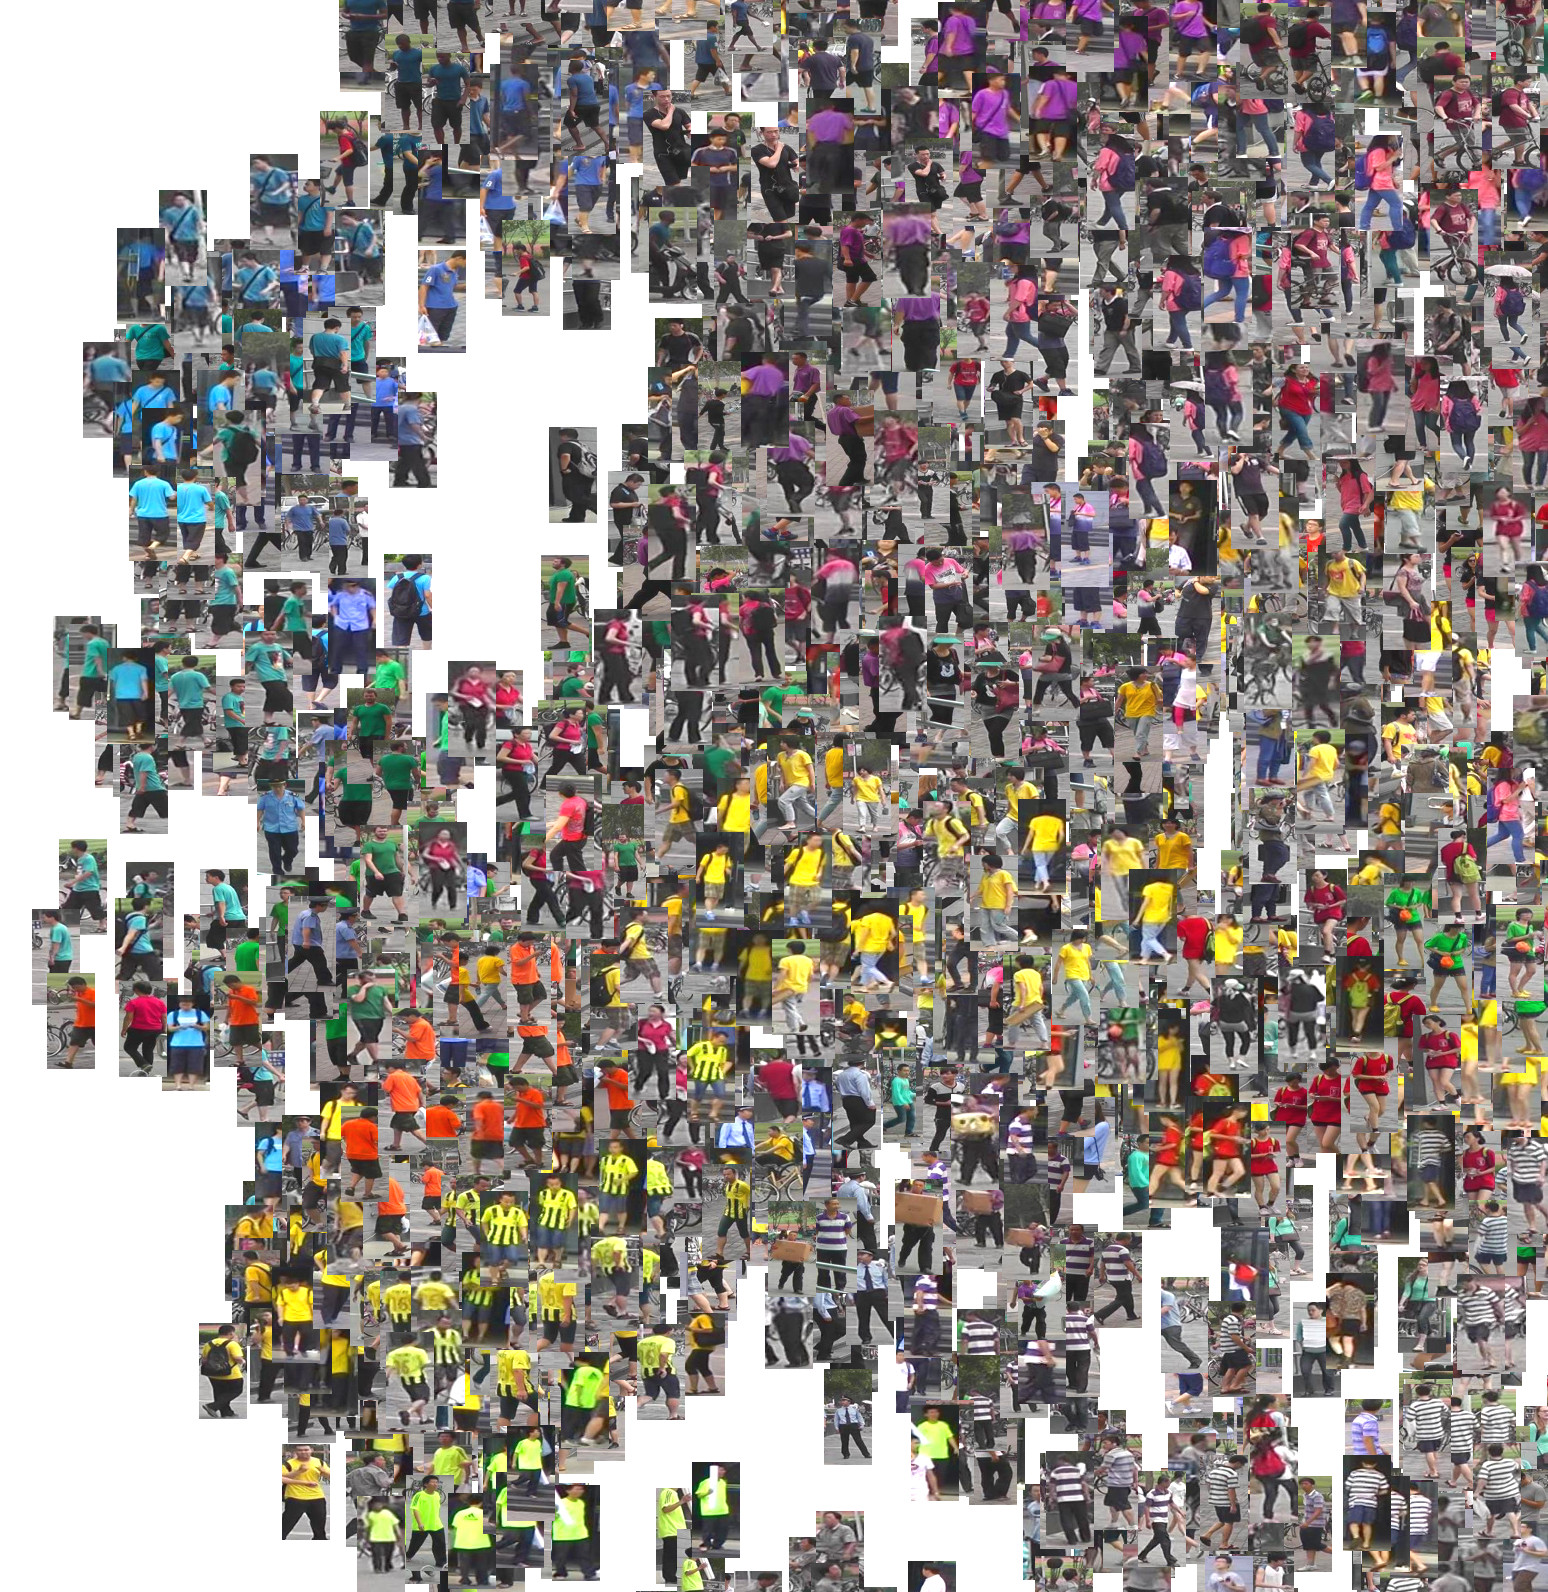
\includegraphics[width=0.6\textwidth]{informatica/embedding_paper_principal}
        \caption{Se representa una porción del \textit{dataset} \textit{Market-1501} tras aplicar el \textit{embedding} aprendido y posteriormente \textit{t-SNE}. Imagen extraída de \cite{informatica:principal}}
    \end{figure}

    Por ejemplo, un modelo que quiera resolver esta tarea podría aprender a mapear personas con exactamente la misma ropa a puntos cercanos.
\end{ejemplo}

\begin{ejemplo}

    Y para finalizar, consideremos nuestra tarea en concreto. Buscamos que las imágenes de la misma persona, aunque hayan pasado los años, se transformen en vectores cercanos. Y al contrario, que imágenes de dos personas distintas estén lo más lejos posible.

    Esto es especialmente complicado, como ya hemos comentando en \sectionref{ich:descrp_problema}, porque por ejemplo, nuestro modelo debe ver como más cercanos imágenes de un niño y un adulto con barba (ambos siendo la misma persona) que dos imágenes de dos adultos con barba (siendo distintas personas). Este problema en concreto lo hemos mostrado en la \imgref{img:messi_distintos_otro_adulto}
\end{ejemplo}


\subsection{\textit{Triplet Loss} como función de pérdida para aprender el \textit{embedding}} \label{isec:triplet_loss}

Ya sabemos que para resolver nuestro problema queremos que un modelo convolucional profundo aprenda un \textit{embedding} semántico que codifique la identidad de las personas independientemente de cambios en la edad. Lo que nos falta es una función de pérdida que optimice los parámetros de nuestro modelo. Justificaremos ahora el uso de \textit{triplet loss} como función de pérdida. Recordemos que estamos trabajando con funciones de la forma:

\begin{equation}
\begin{split}
    f_{\theta}: X & \to \R^N \\
    x & \mapsto f_{\theta}(x)
\end{split}
\end{equation}

y con una función de distancia:

\begin{equation}
\begin{split}
    D: X \times X & \to [0, \infty) \\
    x, y & \mapsto D(x, y)
\end{split}
\end{equation}

Para ser más concisos, usaremos la notación $D_{i, j} := D(f_{\theta}(x_i), f_{\theta}(x_j))$. Como su nombre indica, \textit{triplet loss} trabajará sobre triples. Esto es:

\begin{enumerate}
    \item Una imagen de un individuo concreto, a la que llamaremos \textbf{\textit{anchor}} o ancla
    \item Otra imagen distinta, pero del mismo individuo, a la que llamaremos \textbf{positiva}
    \item Una imagen de un individuo distinto, a la que llamaremos \textbf{negativa}
\end{enumerate}

En este caso, queremos que la distancia entre el \textit{embedding} del ancla y el \textit{embedding} de la positiva (que podemos denotar como $D_{A, P}$) sea mucho menor que la distancia entre el \textit{embedding} del ancla y el \textit{embedding} de la negativa (denotamos $D_{A, N}$). Por tanto, lo que realmente queremos es que:

\begin{equation}
    D_{A, P} \leq D_{A, N}
\end{equation}

o lo que es lo mismo,

\begin{equation}
    D_{A, P} - D_{A, N} \leq 0
\end{equation}

Una forma trivial de hacer que esa ecuación se cumpla, es haciendo que

\begin{equation}
    f(x) = \vec{0}; \dspace \forall x \in X
\end{equation}

con lo que obtendríamos un modelo totalmente inservible. Para evitar eso, introducimos un término $\alpha > 0$ que se conoce como \textbf{margen}, llegando a:

\begin{equation}
    D_{A, P} - D_{A, N} + \alpha \leq 0
\end{equation}

Buscamos que el término de la izquierda sea lo más negativo posible, por lo buscamos minimizar la siguiente función de pérdida:

\begin{equation} \label{ieq:triplet_loss_single_entry}
\begin{split}
    \mathcal{L}_{tri}(\theta; A, P, N) & := max \{D_{A, P} - D_{A, N} + \alpha, 0 \} \\
    &= ReLU(D_{A, P} - D_{A, N} + \alpha)
\end{split}
\end{equation}

Minimizando esta función de pérdida, lo que haremos será atraer elementos de la misma clase entre sí, y alejar elementos de clases distintas. Este proceso se refleja en la siguiente imagen:

\begin{figure}[H]
    \centering
    \includegraphics[width=1.0\textwidth]{informatica/triplet_loss_learning}
    \caption{Ejemplo gráfico del proceso de aprendizaje deseado con \textit{triplet loss}. Imagen creada a partir de datos de \cite{informatica:cacd_dataset} en base a \cite{informatica:facenet}}
\end{figure}

Notar que en \eqref{ieq:triplet_loss_single_entry} trabajamos con una sola entrada de tres datos en forma de imagen. A diferencia de un \textit{dataset} con datos etiquetados clásico, de la forma \lstinline{(entrada, valor de etiqueta)}, tenemos datos de la forma \lstinline{(imagen, identificador de individuo, edad)}. Esto supone un \textbf{problema} a resolver: cómo generamos \textit{batches} con triples de la forma \lstinline{(ancla, positivo, negativo)} para poder aplicar \eqref{ieq:triplet_loss_single_entry}. Explicaremos cómo solucionar esto en \sectionref{isubs:enfoque_offline_minado_triples}

Pero ahora veamos las \textbf{ventajas} que plantea este enfoque. La principal es que, a diferencia de otros enfoques basados en usar funciones de pérdida auxiliares (y que suelen forzar que la red solo pueda funcionar comparando pares de imágenes), el cómputo del \textit{embedding} es directo usando esta función de pérdida (\textit{end to end learning}). Optimizamos directamente la propiedad semántica del \textit{embedding} que deseamos obtener. Una vez entrenado el modelo es directo adaptar el modelo a tareas de \textit{clustering}, \textit{retrieval}, verificación, \ldots \cite{informatica:principal}. En \customref{isubs:impl_retr_adapter} mostramos lo sencillo que es realizar esta adaptación.

\subsubsection{Minado de triples \textit{offline}} \label{isubs:enfoque_offline_minado_triples}

Como ya hemos comentado, la tarea que debemos resolver ahora es la de generación de \textit{batches} adecuados para poder emplear \eqref{ieq:triplet_loss_single_entry} como función de pérdida a minimizar.

Por tanto, dado un conjunto de datos de la forma \lstinline{(imagen, identificador, edad)}, debemos obtener un conjunto de datos de la forma \lstinline{(img. ancla, img. positivo, img. negativo)}. Este último conjunto de datos puede ser una lista de triples o un conjunto de \textit{batches}. Como buscamos trabajar con \textit{batches}, en el caso de tener una lista de triples, podemos simplemente muestrear aleatoriamente y sin remplazo de dicha lista, repitiendo el muestreo tras cada época completada.

El \textbf{minado de triples \textit{offile}} es el enfoque clásico que se ha venido usando previo a \cite{informatica:facenet}, trabajo que introduce un enfoque \textit{online} que luego otros trabajos como \cite{informatica:principal} han ido mejorando. Para entender este minado veamos el ciclo de aprendizaje, que se divide en \textbf{varios pasos}.

En primer lugar, se realiza el minado \textit{offline} de los triples. Es decir, se obtiene una primera lista o conjunto de \textit{batches} de la forma \lstinline{(img. ancla, img.positivo, img.negativo)}. Una forma de hacer esto sería, por ejemplo, generar los triples de forma aleatoria, generar todos los posibles triples, $\ldots\dspace$ Aunque estas ideas no suelen funcionar en la práctica. Otra forma más efectiva es seleccionar los triples en base a algún estudio estadístico. O usar la red que vamos a optimizar para identificar aquellos triples en los que tiene más dificultad.

En segundo lugar, realizamos el aprendizaje sobre dicho conjunto de triples. En algunos casos, realizamos el entrenamiento completo sobre dicho conjunto inicial. En otros casos, principalmente cuando usamos la red para el minado de triples, pasadas algunas épocas de entrenamiento volvemos a generar otra vez la lista de triples. Así, triples que antes la red no identificaba propiamente, ahora sí que los identifica (\entrecomillado{network snapshots}, \cite{informatica:facenet}) y podemos buscar triples más interesantes.

Una vez computado una lista de triples $(a, p, n) \in \Omega$, la función de pérdida \eqref{ieq:triplet_loss_single_entry} se implementa de forma natural como en cualquier otro ámbito de \textit{batching}:

\begin{equation}
    \mathcal{L}_{tri}^{offline}(\theta; \Omega) := \frac{1}{\#\Omega} \sum_{(a, p, n) \in \Omega} \mathcal{L}_{tri}(\theta; a, p, n)
\end{equation}

En la literatura sobre aprendizaje automático normalmente se ignora el término $\frac{1}{\#\Omega}$ y se supone que siempre estamos dividiendo por el número de sumandos, con lo que nuestra función de error suele escribirse como:

\begin{equation}
    \mathcal{L}_{tri}^{offline}(\theta; \Omega) := \sum_{(a, p, n) \in \Omega} \mathcal{L}_{tri}(\theta; a, p, n)
\end{equation}

\subsubsection{Problemas del minado \textit{offline}}

El minado de triples \textit{offline} supone una serie de \textbf{problemas}:

\begin{itemize}
    \item Estamos dividiendo el proceso de aprendizaje en dos etapas, la de minado de triples y la de aprendizaje sobre estos triples. Esto añade complejidad a nuestra \textit{pipeline} (véase \customref{isec:pipeline})
    \item La adecuada elección de triples es fundamental. Si elegimos triples demasiado fáciles, la red no aprenderá nada nuevo, pues es muy fácil distinguir los ejemplos presentados. Sin embargo, si solo mostramos triples complicados, el modelo se centrará en aprender ejemplos extraordinarios y no sabrá distinguir el grueso de ejemplos más sencillos
        \begin{itemize}
            \item Además, generalmente los modelos aprenden rápidamente a distinguir la mayoría de ejemplos en los que las diferencias son relativamente evidentes. Por tanto, en pocas iteraciones la mayoría de triples generados de forma \textit{offline} son demasiado sencillos, lo que agrava mucho el problema que hemos comentado
        \end{itemize}
    \item Sería conveniente disponer de alguna forma de ajustar la complejidad de los triples presentados. Podemos confiar en que al ir re-generando la lista de triples, la complejidad vaya aumentando. Pero el algoritmo de minado debería tener alguna forma de controlar el énfasis que se hace en la búsqueda de combinaciones difíciles, lo que añade aún más complejidad al sistema
    \item El minado supone realizar un proceso de búsqueda, que es \textbf{muy lento} (evaluar de alguna forma todos los posibles triples supondría al menos $O(n^3)$). Lo ideal sería disponer de algún método que se basará en muestrear aleatoriamente de nuestra lista de elementos de la forma \lstinline{(imagen, identidad, edad)} (proceso que es muy rápido) y generar triples interesantes sobre dicho muestreo. Esto motiva la técnica introducida en \sectionref{isubs:triples_online}
\end{itemize}

\section{Mejoras técnicas objeto de estudio}

Hemos introducido todos los conceptos teóricos suficientes para plantear una solución basada en aprendizaje automático para nuestro problema. Sin embargo, una \textbf{parte fundamental de este trabajo consiste en explorar algunas mejoras técnicas} introducidas en \cite{informatica:principal}. Dichas mejoras se resumen en:

\begin{itemize}
    \item Introducir una técnica para minar de forma \textit{online} los triples, basada en el muestreo \textit{PK-Sampling}
    \item A partir del nuevo muestreo podemos definir dos variaciones sobre la función de pérdida
    \item Exploramos el uso de una nueva función de distancia
\end{itemize}

\subsection{Enfoque online de \textit{Triplet Loss}} \label{isubs:triples_online}

Buscamos modificar el minado de triples \textit{offline} para solucionar alguno de sus problemas que hemos comentado. Para ello implementaremos el siguiente proceso. En primer lugar, realizaremos un muestreo aleatorio sobre nuestros datos de la forma \lstinline{(imagen, identidad, edad)}. Este muestreo es rápido y no supone prácticamente tiempo de cómputo. Usando únicamente los datos de ese muestreo, generaremos triples y computaremos la función de pérdida apoyándonos en \eqref{ieq:triplet_loss_single_entry}. Dicha generación ya sí que supone un tiempo de cómputo considerable. Repetimos este proceso hasta agotar todos las entradas de nuestro \textit{dataset}, completando así una época de entrenamiento.

Ya podemos ver algunas \textbf{ventajas de este método}, incluso antes de haber especificado las dos partes fundamentales del proceso (muestreo y selección de triples):

\begin{enumerate}
    \item La ventaja más obvia es que, suponiendo que el tamaño de la muestra es significativamente mucho más pequeño que el tamaño de todo el conjunto de datos, la generación de triples consumirá potencialmente menos tiempo y será más efectiva
        \begin{itemize}
            \item Para afirmar esto rotundamente, tendríamos que realizar un estudio del tiempo del minado \textit{offline} en contraste a la suma de todos los tiempos de minado en cada muestreo
            \item Sin embargo, el tiempo usado es más eficiente, porque en cada muestreo estamos usando la red actualizada. En el minado \textit{offline} podemos gastar muchísimo tiempo en encontrar triples difíciles que, tras entrenar en unos pocos triples previos, acaben siendo sencillos. Por tanto, cuando la red vea triples algo avanzados en la lista, estos ya serán totalmente inútiles
        \end{itemize}
    \item Se facilita en gran parte el ajuste de la dificultad. Podemos buscar triples realmente difíciles, pero como solo se tiene acceso a una pequeña muestra, estamos controlando la dificultad. Así que podemos variar el tamaño de las muestras para buscar un punto medio entre ejemplos muy difíciles o ejemplos demasiado sencillos. Y todo esto sin contar con el factor de que vamos a usar la red actualizada para la elección de los triples
\end{enumerate}

Desarrollada esta visión de forma general, veamos cómo se implementa cada una de las partes, siguiendo las técnicas introducidas en \cite{informatica:principal}.

\subsection{Generación online de \textit{batches} usando \textit{P-K sampling}} \label{isubs:muestreo_datos_pk_sampling_teoria}

La \textbf{idea principal del muestreo} es lo que definiremos como \textbf{\textit{P-K sampling}}. Como ya hemos comentado en \sectionref{isubs:triples_online}, nuestra tarea ahora es generar un \textit{batch} de elementos de la forma \lstinline{(imagen, identidad, edad)}. En una segunda etapa (véase \sectionref{isubs:seleccion_de_triples}), otro algoritmo decide cómo generar triples a partir de estos datos.

El algoritmo de muestreo \textit{P-K sampling} es muy sencillo. En cada muestreo, seleccionamos aleatoriamente $P$ identidades de individuos (o clases, en un ambiente más general en el que no necesariamente estemos trabajando con imágenes de personas). Por cada una de las identidades, seleccionamos aleatoriamente $K$ imágenes asociadas a esa identidad. Por tanto, obtenemos una lista de $P \cdot K$ imágenes, a la que llamaremos \textbf{\textit{P-K batch}}. Para poder obtener triples interesantes en la siguiente etapa, parece que lo deseable es que ambos muestreos aleatorios sean sin repetición.

El hecho de tener $K$ imágenes por cada uno de los individuos seleccionados es lo que va a permitir al algoritmo de generación de triples obtener rápidamente triples interesantes.

\begin{figure}[H]
    \centering
    \includegraphics[width=0.6\textwidth]{informatica/ejemplo_grafico_pk_sampling}
    \caption{Ejemplo gráfico del proceso de \textit{P-K sampling}. Imagen extraída de \cite{informatica:paper_image_pk_sampling}}
\end{figure}

Queda aquí claro el \textbf{problema principal} que introduce esta técnica: si queremos muestrear $K$ imágenes de cada individuo sin repetición, cada individuo debe tener asociadas al menos $K$ imágenes. Así que a la hora de trabajar con un \textit{dataset}, siempre deberíamos comprobar la distribución del número de imágenes por individuo, como haremos en \sectionref{isec:base_datos_usada}.

\subsection{Selección de triples y variaciones en la función de pérdida} \label{isubs:seleccion_de_triples}

Una vez que tenemos un \textit{batch} de $P \cdot K$ elementos, deberemos generar una lista de triples en base a este \textit{batch}. Una vez se especifica cómo se seleccionan los triples, usando \eqref{ieq:triplet_loss_single_entry}, inducimos de forma natural y directa una cierta función de pérdida que actúa sobre estos \textit{P-K batches}.

Introducimos una notación que nos va a ser útil. Trabajamos $P \cdot K$ elementos, cada uno correspondiendo a una clase en concreto. Por tanto, indexaremos los elementos de la forma $x_k^p$ donde $p$ marca el identificador del individuo, y $k$ marca a cuál de las $K$ imágenes del individuo $p$ nos estamos refiriendo

\subsubsection{\textit{Batch Hard}} \label{isubsubs:batch_hard}

La primera idea es iterar sobre todos los elementos del \textit{P-K batch}, obteniendo así $P \cdot K$ anclas. Por cada ancla, seleccionamos el positivo y negativo \textbf{más complicado dentro de \textit{P-K batch}}. Por tanto, queda claro que \textbf{estamos usando la red para seleccionar triples difíciles} en cada \textit{batch} generado.

Esto introduce la siguiente función de pérdida, a la que llamaremos \textbf{\textit{Batch Hard}}:

\begin{equation}
    \mathcal{L}_{BH}(\theta, \hat{\Omega}) := \comentarencima{\sum_{p = 1}^P \sum_{k = 1}^K}{\text{todas las anclas}} [
        \comentarencima{\max_{k' = 1, \ldots, K} D(f_{\theta}(x_k^p), f_{\theta}(x_{k'}^p))}{\text{positivo más complicado}}
        - \comentarencima{\min_{\substack{p' = 1, \ldots, P \\ p' \neq p \\ k' = 1, \ldots, K}} D(f_{\theta}(x_k^p), f_{\theta}(x_{k'}^{p'}))}{\text{negativo más complicado}}
        + \alpha]_+
\end{equation}

donde $[x]_+ := max \{0, x\} = ReLU(x)$ y $\hat{\Omega}$ se refiere a un \textit{P-K batch}. No olvidemos que no estamos escribiendo la división por el número de sumandos, $P \cdot K$.

Estamos generando \textbf{triples moderados}, porque estamos buscando los triples más difíciles, pero dentro de un \textit{batch} relativamente pequeño comparado a el total del conjunto de datos. Con esto estamos ajustando la dificultad de los triples cómodamente, resolviendo el problema que comentábamos en \sectionref{isubs:enfoque_offline_minado_triples}. Aumentando el valor de $\{P, K\}$ aumentamos el tamaño del espacio de búsqueda, y por tanto podremos encontrar triples mucho más difíciles. Sin embargo, hay que tener siempre en cuenta el coste en tiempo de cómputo.

Queda claro que, gracias al proceso de \textit{P-K sampling}, ahora es factible realizar una búsqueda de triples interesantes en profundidad, basándonos en el estado más actualizado de la red para calcular la dificultad de los triples. Esta búsqueda extensiva no habría sido posible si la planteásemos sobre todo el conjunto de datos.

\subsubsection{\textit{Batch All}} \label{isubsubs:batch_all}

Motivados por lo que acabamos de comentar en \sectionref{isubsubs:batch_hard}, podemos plantearnos usar todos los posibles triples dentro de un \textit{P-K batch} como un enfoque que ahora cobra más sentido (ya hemos comentado en \sectionref{isubs:enfoque_offline_minado_triples} que realizar esto sobre todo el conjunto de datos no parece una buena idea).

Realizar esto introduce la función de pérdida que llamaremos \textbf{\textit{Batch All}}:

\begin{equation} \label{ieq:batch_all}
    \mathcal{L}_{BA}(\theta; \hat{\Omega}) :=
    \comentarencima{\sum_{p = 1}^{P} \sum_{k = 1}^K}{\text{todas anclas}}
    \comentardebajo{\sum_{\substack{k' = 1 \\ k' \neq k}}^{K}}{\text{todas pos.}}
    \comentarencima{\sum_{\substack{p' = 1 \\ p' \neq p}}^P \sum_{n = 1}^K}{\text{todas neg.}} \dspace[
        D(f_{\theta}(x_k^p),f_{\theta}(x_{k'}^p)) - D(f_{\theta}(x_k^p),f_{\theta}(x_{n}^{p'})) + \alpha
    ]_+
\end{equation}

Está claro que, por el número de sumandos, esta aproximación es viable gracias a que nuestro \textit{P-K sampling} reduce mucho el número de elementos sobre los que operamos. Dicho número de sumandos viene dado por:

\begin{equation}
    P \cdot K \cdot (K - 1) \cdot (P - 1) \cdot K = P^2 - P + K^3 - K^2 \approx P^2 + K^3
\end{equation}

Esta aproximación sería completamente inviable sobre un número muy elevado de elementos. Pensemos, por ejemplo, en las 163446 imágenes de \textit{CACD} (conjunto de datos que estudiamos en \sectionref{isec:dataset_cacd}).

\subsubsection{Mejoras introducidas a partir de la experimentación} \label{isubsubs:mejoras_sumandos_no_nulos}

En \cite{informatica:principal}, a raíz de observar los resultados de la experimentación, señalan algunos puntos débiles en las dos funciones de pérdida que introducen a partir del \textit{P-K sampling}.

Principalmente, en \customref{isubsubs:batch_all}, podemos ver un posible fallo en la función de pérdida \eqref{ieq:batch_all}. Si se da el caso de que la mayoría de triples generados son fáciles (hecho muy probable al estar generando todas las combinaciones de triples), los escasos triples que realmente son difíciles se desvanecerán. Esto porque la mayoría de términos serán cero (al estar aplicando $[x]_+$). Y los pocos términos que no son cero, se dividen por el número total de elementos, que ya hemos visto que es elevado.

Por tanto, una mejora sencilla a esta función de pérdida es dividir únicamente por el número de sumandos no nulos. A estos sumandos no nulos también se les llama sumandos activos \cite{informatica:principal}. Esta mejora la podemos aplicar también a \textit{batch hard}, obteniendo dos nuevas funciones de pérdida, a las que denotaremos por $\mathcal{L}_{BA \neq 0}$ y $\mathcal{L}_{BH \neq 0}$.

\subsubsection{Algunas observaciones y conclusiones} \label{isubsubs:observaciones_conclusiones_pksampling}

En primer lugar, cabe destacar que, como señalan \cite{informatica:principal}, las dos nuevas funciones de pérdida introducidas equivalen al planteamiento clásico de \textit{triplet loss} si entrenásemos indefinidamente.

El desarrollo que hemos realizado justifica las siguientes \textbf{ventajas} de los nuevos métodos:

\begin{itemize}
    \item El uso del \textit{P-K sampling} y las dos nuevas funciones de pérdida (con las variantes técnicas que consideran los sumandos activos) permite realizar un aprendizaje \textit{end-to-end}, sin añadir un paso adicional en el bucle de aprendizaje, evitando así la gran complejidad añadida del minado \textit{offline}
    \item Además, conseguimos un manejo preciso de la dificultad de los triples obtenidos. Controlando el valor de $\{P, K\}$, controlamos el espacio de búsqueda y, en definitiva, la dificultad. Todo esto de forma cómoda y sin introducir apenas complejidad en nuestro \textit{pipeline}
    \item Aunque no lo hemos comprobado, pensamos que esto acelera los tiempos de cómputo, al estar realizando el minado de triples sobre \textit{batches} de tamaño considerablemente reducidos
    \item Y aunque no mejorásemos el tiempo de computo, lo que sí sabemos que mejoramos es la eficacia del minado de triples. El minado de triples \textit{online} usa una red mucho más actualizada, para generar una lista mucho más pequeña que probablemente no se degrade tanto como la generada por un minado \textit{offline} sobre todo el conjunto de datos, mucho más grande
    \item Es más, estamos controlando el efecto de los triples demasiado sencillos, que no tendremos en cuenta a la hora de promediar en la función de pérdida
\end{itemize}

A pesar de esto, a raíz de trabajar con estas nuevas técnicas, identificamos los siguientes \textbf{inconvenientes}:

\begin{itemize}
    \item Introducimos dos hiperparámetros, $\{P, K\}$ que deberemos ajustar correctamente, pues tienen un enorme impacto en los resultados del proceso de entrenamiento. Por tanto, se hace fundamental tener un proceso de \textit{hyperparameter tuning} robusto, como introducimos en \sectionref{isec:hptuning_kfold_cross_validation} e implementamos en \sectionref{isec:hp_tuning}
    \item Tenemos que tener mucho cuidado con usar valores elevados de $\{P, K\}$ por dos motivos. El primero, y como ya hemos comentado, valores altos implicarán que los tiempos de cómputo para la generación de triples crecerán rápidamente. El segundo es que el tamaño de los \textit{batches} crecerán considerablemente, llegando a colapsar la memoria disponible de la \textit{GPU}
    \item Hemos comprobado en la práctica que es realmente fácil colapsar la memoria \textit{GPU}, usando modelos profundos como \textit{ResNet50} con valores de $P \cdot K = 100$. Esto supone que, aunque no estuviéramos limitados por el tiempo de cómputo, el colapso de la memoria limita el conjunto de valores $\{P, K\}$ con los que podemos experimentar
    \item Si queremos usar valores altos de $K$, nuestro \textit{dataset} lo debe permitir, teniendo una buena distribución de imágenes por individuo. Por este motivo hemos estudiado esta distribución en \sectionref{isec:base_datos_usada}. Se pueden explorar técnicas como el aumentado de datos para alcanzar el número de imágenes por individuo deseado, pero solo serán efectivas si dicha distribución es buena para empezar (véase \sectionref{isec:aumentado_datos})
    \item Tanto por el formato de los datos con los que hemos trabajado, como por el cambio fundamental realizado en el \textit{sampling} de los datos, hemos tenido que realizar un \textbf{esfuerzo considerable de implementación}, al no poder basarnos en la mayor parte de los casos en código implementado por alguna biblioteca de aprendizaje automático. Esto se ve reflejado en \sectionref{ich:implementacion}
\end{itemize}

\subsection{Variaciones en la función de distancia}

En todos los conceptos que hemos ido introduciendo la función de distancia

\begin{equation}
    D: X \times X \to [0, \infty)
\end{equation}

ha estado presente, pero todavía no hemos introducido ninguna función concreta. En el ambiente de \textit{AIFR} se suele usar la distancia euclídea al cuadrado, esto es:

\begin{equation}
    D(x_i, x_j) := ||f_{\theta}(x_i) - f_{\theta}(x_j)||^2_2
\end{equation}

Sin embargo, motivados por \cite{informatica:principal}, decidimos usar la distancia euclídea usual. En este trabajo se afirma que, en base a la experimentación, de esta forma se obtienen entrenamientos más estables. Además, usando la distancia euclídea usual, el margen es más fácil de interpretar, porque marca la diferencia de distancias, y no la diferencia de cuadrados de distancias. Por lo tanto, en base a dicho trabajo, decidimos tomar:

\begin{equation}
        D(x_i, x_j) := ||f_{\theta}(x_i) - f_{\theta}(x_j)||_2
\end{equation}

\subsection{Márgenes suaves} \label{isec:margenes_suaves}

En \sectionref{isec:triplet_loss} hemos justificado por qué es necesario introducir un término $\alpha$ para controlar el margen y evitar que nuestro modelo aprenda a colapsar todas las entradas al vector $\vec{0}$. Con esto llegamos a la ecuación \eqref{ieq:triplet_loss_single_entry}.

En dicha función de pérdida, el propósito de $x \mapsto \max\{0, x + \alpha\}$ (conocida comúnmente como \textit{hinge function}) es no corregir ejemplos que, en vista del margen $\alpha$ establecido, ya son correctos. Pero puede ser que estemos interesados en afinar aún más ejemplos que, para dicho valor del margen, sean correctos. Con esto conseguiríamos seguir acercando imágenes del mismo individuo lo máximo posible \cite{informatica:principal}. Es por esto que se propone en usar la función \textbf{\textit{softplus}}:

\begin{equation}
    x \mapsto ln(1 + exp(x))
\end{equation}

Dicha función puede verse como una versión suavizada de la función \textit{hinge}. Decae exponencialmente, por lo que ejemplos correctos se penalizarán exponencialmente menos cuanto más cercanos estén, pero contrasta con la función \textit{hinge} en que no presenta un salto o corte fuerte. Por tanto, se suele decir que estamos usando un \textbf{margen suave}. Además, una ventaja de esta función es que \textbf{desechamos el hiperparámetro $\alpha$}, el cual ya no tenemos que fijar a través de algún método (como podría ser el \textit{hyperparameter tuning}).

\begin{figure}[H]
\centering
    \begin{subfigure}{.5\textwidth}
        \centering
        \includegraphics[width=0.8\linewidth]{informatica/desmos_hinge}
        \caption{Función \textit{hinge} con $\alpha = 2$}
    \end{subfigure}%
    \begin{subfigure}{.5\textwidth}
        \centering
        \includegraphics[width=0.8\linewidth]{informatica/desmos_softplus}
        \caption{Función \textit{softplus}}
    \end{subfigure}

    \begin{subfigure}{.5\textwidth}
        \centering
        \includegraphics[width=0.8\linewidth]{informatica/desmos_conjunta}
        \caption{En azul, \textit{hinge} con $alpha = 0$. En rojo, \textit{softplus}}
    \end{subfigure}


\caption{Gráfica de las dos funciones para trabajar con los márgenes, y una gráfica conjunta que muestra su similitud}
    \label{img:graficas_margenes}
\end{figure}

Las gráficas mostradas en \imgref{img:graficas_margenes} nos sirven para visualizar de forma sencilla todo lo que hemos comentado. La función \textit{softplus} actúa como una \textit{hinge} suavizada. El hecho de que se parezcan tanto cuando hacemos que el margen de \textit{hinge} sea cero nos hace pensar que \textit{softplus} va a actuar como una \textit{hinge} en la que no hay margen, y por lo tanto, acercará elementos de la misma clase todo lo que pueda.


\chapter{Modelización de la tarea de aprendizaje} \label{ch:tarea_aprendizaje}

La tarea de aprendizaje que consideramos es la de clasificación. Durante todo el desarrollo, pensaremos en la \textbf{clasificación de imágenes}. En este caso, el enfoque que más éxito ha tenido históricamente es el uso de redes convolucionales profundas y, más actualmente, el uso del modelo \entrecomillado{transformer}.

Dado un elemento $X = (\nv{x_1}, \ldots, \nv{x_N})$, donde $\nv{x_i} \in \R^s \ \forall i \in \deltaset{N}$, queremos clasificarlo en alguna de las etiquetas $\mathcal{Y} = \{1, \ldots, Y \} = \deltaset{Y}$.

Con esto, podemos ver que los datos de entrada viven en el espacio

$$\mathcal{X} := \R^s \times \overset{N}{\ldots} \times \R^s = (R^s)^N$$

Esta representación de los datos de entrada es natural en muchas situaciones. En el caso de las imágenes, podemos considerar cada vector $\nv{x_i}$ como un conjunto de \textit{pixels} de la imagen. Idealmente, cada vector de \textit{pixels} debería contener un vecindario de \textit{pixels}, es decir, \textit{pixels} adyacentes. Podemos incluso considerar \textit{pixels} que aparezcan en más de un vector. Por ejemplo, podemos considerar $\nv{x_i}$ como la fila o columna $i$-ésima de la imagen.

Por ejemplo, el trabajo que presenta el conocido modelo  de deep learning \textit{VIT} propone una arquitectura \entrecomillado{transformer} a la que que se le pasa \entrecomillado{patches} de la imagen para poder explotar el mecanismo de atención: \entrecomillado{we split an image into patches and provide the sequence of linear embeddings of these patches as an input to a Transformer} \footnote{\cite{matematicas:vit}}
\todo{No sé si así está bien referenciado el trabajo al que me refiero}

Para decidir la etiqueta de un elemento, consideramos $Y$ \textbf{funciones de puntuación}:

$$\{h_y: \mathcal{X} \to \R \dspace / \dspace y \in \mathcal{Y} \}$$

Con esto, dado un elemento $X \in \mathcal{X}$, lo clasificaremos buscando la etiqueta cuya función de puntuación sea máxima, es decir:

$$\hat{y} := \underset{y \in \mathcal{Y}}{argmax} \dspace h_y(X)$$

Por tanto, nuestro \textbf{espacio de hipótesis} $\Gamma$ es el conjunto de funciones $\mathcal{X} \to \R$. Tanto en la práctica con modelos de \textit{machine learning}, como en nuestras dos modelizaciones, trabajamos en un subconjunto $\tilde{\Gamma} \subset \Gamma$ de funciones de puntuación, implementables o bien por el modelo de \textit{machine learning} o bien por nuestra modelización teórica.

\section{Espacio de hipótesis general}

\subsection{Justificación para la representación de las funciones de puntuación} \label{sec:justificacion_func_repr}

\todo{Desarrollar el apéndice 6 donde se justifica que esta ecuación es lo suficientemente general}

\subsection{Representación de las funciones de puntuación} \label{sec:repr_funciones_puntuacion}

Por todo esto, las funciones de puntuación vendrán dadas de la forma:

\begin{equation} \label{eq:puntuacion_general}
    h_y(\nv{x_1}, \ldots, \nv{x_N}) = \sum_{d_1, \ldots, d_N = 1}^{M} \mathcal{A}^y_{d_1, \ldots, d_N} \prod_{i = 1}^N f_{\theta_{d_i}}(\nv{x_i})
\end{equation}

Explicamos ahora algunos detalles sobre esta ecuación, que será central en nuestro trabajo.

En primer lugar, usamos la notación $\sum_{d_1, \ldots, d_N = 1}^{M}$ para denotar $\sum_{d_1 = 1}^{M} \sum_{d_2 = 1}^{M} \ldots \sum_{d_N = 1}^{M}$

Las funciones $f_{\theta_1}, \ldots, f_{\theta_M}: \R^s \to \R$ son las \textbf{funciones de representación}. Cada una de estas funciones se selecciona de una familia paramétrica

$$\mathcal{F} = \{ f_{\theta}: \R^s \to \R / \theta \in \Theta \}$$

Algunas funciones de representación usuales son:

\begin{itemize}
    \item \textit{Wavelets}
    \item Funciones de base radial (\textit{RBF}), normalmente la Gaussiana
    \item Neuronas
\end{itemize}

El tensor $\mathcal{A}^y$ será el \textbf{tensor de coeficientes}. Por la sumatoria en \eqref{eq:puntuacion_general}, es claro que tiene orden $N$ y dimensión $M$ en cada modo. Es decir, $\mathcal{A} \in \espaciotensores{N}{M}$.

La tarea de aprendizaje ahora será aprender los valores de los parámetros $\theta_1, \ldots, \theta_M$ y los valores de los tensores de coeficientes $\mathcal{A}^1, \ldots, \mathcal{A}^Y$.

\begin{observacion}

    Estamos usando las mismas funciones de representación $f_{\theta_1}, \ldots, f_{\theta_M}: \R^s \to \R$ para todas las funciones de representación $h_y, y \in \mathcal{Y}$, lo único que cambia entre las distintas funciones de puntuación es el tensor de coeficientes $\mathcal{A}^y$.


    Notar además que en la ecuación \refeq{eq:puntuacion_general}, los vectores de entrada $\nv{x_i}$ solo participan en el productorio que involucra computar $f_{\theta_{d_i}}(\mathbf{x_i})$.

    Por tanto, aunque esto se corresponda más con el posterior diseño de las redes neuronales que vamos a realizar, podemos considerar como paso inicial, compartido en los dos modelos que proponemos, el cómputo de los valores:

    $$\{f_{\theta_d}(\nv{x_i}) / d \in \deltaset{M},\ i \in \deltaset{N} \}$$

    Una vez que hayamos computado esos $M \cdot N$ valores, ya no necesitamos los valores $\nv{x_i}$ para nada más. Con esto, es natural considerar que nuestro modelo tenga una primera capa que compute esos valores. Podemos considerar dicha capa como una \textbf{primera capa convolucional} con $M$ canales, a la que llamaremos \textbf{capa de representación}.

    Y como ya hemos comentado, estamos usando las mismas funciones de representación para las $Y$ funciones de puntuación. Por tanto, fijados los parámetros $\theta_i$, en todas las funciones de puntuación la capa de representación será la misma.
\end{observacion}

\begin{observacion}
    Sabemos, por lo comentado en \customref{sec:justificacion_func_repr}, que al trabajar con \textit{wavelets}, \textit{RBFs} y neuronas, podemos extraer un conjunto numerable de funciones que sea total y linealmente independiente. También gracias a \customref{sec:justificacion_func_repr}, que por tanto el siguiente espacio de funciones es total y linealmente independiente:
    \todo{Tengo que mirar esto bien. Creo que aquí es cuando discuten el valor de $M$ para saber que me vale con un subconjunto finito de funciones de representación. \textbf{MIRAR BIEN}}

    $$\{(\nv{x_1}, \ldots, \nv{x_N}) \mapsto \prod_{i = 1}^{N} f_{\theta_{d_i}} (\nv{x_i}) \dspace / \dspace d_i \in \deltaset{M} \dspace \forall i \in \deltaset{N}\}$$

    Por tanto, actúa de forma parecida a una base de un espacio vectorial. Teniendo en cuenta este comportamiento similar, podemos pensar que el tensor $\mathcal{A}^y$ nos da los coeficientes de la función de puntuación $h_y$ en dicha \entrecomillado{base}.

    \todo{Tengo que desarrollar bien esa sección para justificar todas estas cosas que estoy diciendo}
\end{observacion}

\begin{observacion}
    Como ya sabemos, como $\mathcal{A} \in \espaciotensores{N}{M}$, tenemos que optimizar el valor de $M^N$ valores reales a través del proceso de aprendizaje. Esto supone un reto, que \textbf{motiva el uso de los dos modelos}, que se basarán en descomposiciones tensoriales para que el aprendizaje del tensor de coeficientes sea más factible.
    \todo{Tengo que comentar en la introducción que el número de elementos de un tensor N, M es M elevado a N}
\end{observacion}

\endinput

\chapter{Modelización de las redes neuronales} \label{ch:modelizacion}

A partir de las herramientas matemáticas que hemos introducido en \customref{ch:matematicas_fundamentales} y de la modelización de la tarea de aprendizaje realizada en \customref{ch:tarea_aprendizaje}, buscamos desarrollar una modelización matemática de las redes neuronales con las que se suele trabajar en la práctica. Para que sea una \textbf{buena modelización}, esta debería cumplir que:

\begin{itemize}
	\item Sea lo más parecida a los modelos que se usan en la práctica.
	\item Permita obtener resultados interesantes.
\end{itemize}

Usando descomposiciones tensoriales, modelaremos dos tipos de redes:

\begin{itemize}
	\item Redes neuronales no profundas, a partir de la descomposición \textit{CANDECOMP/PARAFAC} o descomposición \textit{CP}.
	\item Redes convolucionales profundas, a partir de la descomposición jerárquica de \textit{Tucker} o descomposición \textit{HT} por sus siglas en inglés.
\end{itemize}

Las \textbf{modelizaciones son muy cercanas a las arquitecturas usadas en la práctica del aprendizaje automático}. Principalmente, porque tienen en cuenta las tres propiedades características de una red convolucional:

\begin{enumerate}
	\item Localidad.
	\item Compartición de parámetros, que junto a la localidad, da lugar a la convolución.
	\item \textit{Pooling}.
\end{enumerate}
\todo{Desarrollar de forma más extensa qué significan estas propiedades. Antes digo que voy a explicar qué son estas propiedades. Y además, estoy repitiendo el listado, por lo que tengo que desarrollar bien estas propiedades}

\section{Modelo \textit{CP}}

Este modelo será el resultado de aplicar la descomposición tensorial \textit{CP} en la función de puntuación dada por \eqref{eq:puntuacion_general}. Como veremos más adelante, esto resultará en un modelo \textit{shallow}, con una única capa convolucional oculta.

\subsection{Descomposición CANDECOMP/PARAFAC} \label{subs:descomposcion_cp}

En esta sección introduciremos la descomposición tensorial \textit{CANDECOMP/PARAFAC}. Esta es la descomposición más sencilla de las dos descomposiciones que vamos a manejar. Empecemos introduciendo la siguiente propiedad sobre los tensores puros:

\begin{proposicion}[Rango matricial de los tensores puros]
	Sean $\nv{v} \in \R^{N}, \nv{w} \in \R^{M}$ dos vectores. Entonces su producto tensorial puede expresarse como:

	$$\nv{v} \otimes \nv{w} = \nv{v} \nv{w}^T \in \espaciomatrices{N}{M}$$

	Además, esta matriz es de rango uno o cero (este último caso ocurre únicamente cuando alguno de los dos vectores es $\vec{0}$)
\end{proposicion}

\begin{proof}

	Sean $\nv{v} = (v_1, \ldots, v_N)$ y $\nv{w} = (w_1, \ldots, w_M)$ dos vectores cualesquiera. Entonces, usando la expresión del producto tensorial que introducimos en \customref{sec:otra_forma_tensores}, tenemos que:

	\begin{equation}
		\nv{v} \otimes \nv{w} = (v_i w_j)_{i \in \deltaset{N},\ j \in \deltaset{M}}
	\end{equation}

	O lo que es lo mismo:

	\begin{equation}
		\nv{v} \otimes \nv{w} = \begin{pmatrix}
			v_1 w_1 & v_1 w_2 & \ldots & v_1 w_M \\
			v_2 w_1 & v_2 w_2 & \ldots & v_1 w_M \\
			\vdots  & \vdots  &        & \vdots  \\
			v_N w_1 & v_N w_2 & \ldots & v_N w_M \\
		\end{pmatrix}
	\end{equation}

	Que claramente se corresponde con la expresión de $\nv{v} \nv{w}^T$. Además, es claro que la fila $i$-ésima viene dada por el vector fila

	$$(v_i w_1, v_i w_2, \ldots, v_i w_M) = v_i (w_1, \ldots, w_M) = v_i \nv{w}^T$$

	Por tanto, todas las filas son combinación lineal de una de las filas.

	En el caso de que alguno de los dos vectores $\nv{v}$ o $\nv{w}$ sea $\vec{0}$, tenemos que la matriz $\nv{v} \otimes \nv{w}$ es la matriz de ceros, y por tanto su rango es cero.

	Estudiado ese caso, ahora podemos suponer que $\nv{v}, \nv{w} \neq \vec{0}$, y por tanto se debe cumplir que $\exists i_0 \in \deltaset{N}: v_{i_0} \neq 0$. Esa será la fila que escogemos para expresar el resto de filas como combinación lineal de esta, aprovechando de que es no nula. Dicha fila se puede expresar como $v_{i_0} \nv{w}^T$. La fila $i$-ésima se puede expresar como $v_i \nv{w}^T$. Y por tanto:

	\begin{equation}
		\begin{split}
			v_i \nv{w}^T = \lambda \cdot v_{i_0} \nv{w}^T \iif & \lambda = \frac{v_i}{v_{i_0}} \\
			& \lambda \neq 0 \iif v_i \neq 0
		\end{split}
	\end{equation}

	Con esto sabemos que $rank(\nv{v} \otimes \nv{w}) \leq 1$, pero podría darse el caso de que el rango fuese cero aún siendo $\nv{v}, \nv{w} \neq \vec{0}$. Sin embargo, esto no es posible. Como $\nv{v}, \nv{w} \neq \vec{0}$, entonces $\exists i_0 \in \deltaset{N}, \exists j_0 \in \deltaset{M}$ de modo que $v_{i_0}, w_{j_0} \neq 0$. Por tanto, el menor de orden 1 asociado a la fila $i_0$-ésima y columna $j_0$-ésima tiene el valor $v_{i_0} w_{j_0} \neq 0$, y con ello, $rank(\nv{v} \otimes \nv{w}) \geq 1$.

\end{proof}

\begin{observacion}
	Estamos escribiendo la igualdad $\nv{v} \otimes \nv{w} = \nv{v} \nv{w}^T$ sin definir lo que significa la igualdad entre un tensor de orden 2 y una matriz. Sin embargo, esta igualdad es totalmente natural. Decimos que un tensor de orden dos y una matriz son iguales cuando las dimensiones de la matriz y las dos dimensiones del tensor coinciden, y cuando las entradas de ambos coinciden.
\end{observacion}

La anterior proposición muestra que los tensores puros que vienen dados como producto tensorial de dos vectores tienen un rango matricial igual a uno (en caso de que no sean ambos vectores nulos). Es natural plantearse generalizar esta propiedad a tensores puros que vengan dados como producto tensorial de $N$ vectores. Pero de momento no tenemos una herramienta para comparar tensores de orden $N > 2$ con matrices. Esto motiva la introducción de la descomposición tensorial \textit{CANDECOMP/PARAFAC}:

\begin{proposicion}[\textbf{Descomposición \textit{CANDECOMP/PARAFAC}}]
	Todo tensor $\mathcal{A}$ puede ser expresado como la suma de tensores puros. Es decir, $\forall \mathcal{A} \in \R^{M_1 \times \cdots \times M_N}$, $\exists Z \in \N$:

	\begin{equation} \label{eq:cp_decomp}
		\mathcal{A} = \sum_{i = 1}^Z \nv{v_i^{(1)}} \otimes \cdots \otimes \nv{v_i^{(N)}};
		\qquad \nv{v_i^{(k)}} \in \R^{M_k},
		\dspace \forall i \in \deltaset{Z},
		\dspace \forall k \in \deltaset{N},
	\end{equation}
\end{proposicion}

\begin{observacion}[Origen del nombre de la descomposición]
	En 1927 Hitchcock propone la idea de expresar un tensor como la suma de tensores de rango uno. En 1970 se introducen dos trabajos independientes que resuelven esta tarea. El primero, introducido por Carol y Chang, propone la descomposición canónica (\textit{CANonical DECOMPosition} o \textit{CANDECOMP}). El segundo trabajo, introducido por Harshman, propone la descomposición por factores paralelos (\textit{PARallel FACtors} o \textit{PARAFAC}). Más tarde se descubre que ambas descomposiciones son equivalentes, por lo que se adopta el nombre conjunto \cite{matematicas:cp_nombre_paper}.
\end{observacion}

\begin{observacion}
	Esta descomposición es equivalente a la siguiente descomposición:

	\begin{equation}
		\mathcal{A} = \sum_{i = 1}^Z \lambda_i \cdot \nv{v_i^{(1)}} \otimes \cdots \otimes \nv{v_i^{(N)}};
		\qquad \nv{v_i^{(k)}} \in \R^{M_k},
		\dspace \lambda_i \in \R,
		\dspace \forall i \in \deltaset{Z},
		\dspace \forall k \in \deltaset{N},
		\dspace Z \in \N
	\end{equation}

	Puesto que podemos considerar:

	\begin{equation}
		\nv{w_i^{(1)}} := \lambda_i \cdot \nv{v_i^{(1)}} \in \R^{M_1}
	\end{equation}

	y usando de nuevo las propiedades del producto tensorial:

	\begin{equation}
		\lambda_i \cdot \nv{v_i^{(1)}} \otimes \nv{v_i^{(2)}} \otimes \cdots \otimes \nv{v_i^{(N)}} = \nv{w_i^{(1)}} \otimes \nv{v_i^{(2)}} \otimes \cdots \otimes  \nv{v_i^{(N)}}
	\end{equation}
\end{observacion}

\begin{observacion}
	Nótese que el número de vectores que multiplicamos tensorialmente es constante, no varía dicho número de vectores entre sumandos. Y dicho número coincide con el orden $N$ del tensor que estemos construyendo.
\end{observacion}

\begin{proof} \label{proof:demostracion_cp_es_universal}
	% TODO -- seguir por aqui
	Queremos descomponer el tensor $\mathcal{A}$ que tiene orden $N$ y dimensión $M_k$ en cada dimensión $k \in \deltaset{N}$. Por tanto, $\mathcal{A}$ tiene $M_1 \cdot M_2 \cdot \ldots \cdot M_N$ elementos. En base a esto, tomamos $Z = M_1 \cdot M_2 \cdot \ldots \cdot M_N$ y en cada sumando de la descomposición buscamos colocar un único coeficiente del tensor en su índice correspondiente.

	Por tanto, en cada sumando buscamos encontrar vectores cuyo producto tensorial genere un tensor, de dimensiones adecuadas, con todas las entradas nulas salvo la entrada de la que nos ocupamos en esa iteración.

	Para que la demostración sea más clara cambiaremos la forma de indexar la suma. En la proposición estamos usando un único índice que llega hasta $Z = M_1 \cdot \ldots \cdot M_N$. Esto es lo mismo que usar $N$ índices que lleguen hasta $M_k$, y así la sumatoria queda:

	\begin{equation}
		\mathcal{A} = \sum_{d_1 = 1}^{M_1} \sum_{d_2 = 1}^{M_2} \cdots \sum_{d_N = 1}^{M_N} \lambda_{i_1, \ldots, i_N} \cdot \nv{v_{(i_1, \ldots, i_N)}^{(1)}} \otimes \ldots \otimes \nv{v_{(i_1, \ldots, i_N)}^{(N)}}
	\end{equation}

	Para llevar a cabo la idea de usar cada sumando para colocar un elemento de $\mathcal{A}$ en sus índices correctos, haremos que en cada sumando se verifique

	\begin{itemize}
		\item $\lambda_{i_1, \ldots, i_N} = \mathcal{A}_{i_1, \ldots, i_N}$. Esto es inmediato y no necesita más explicación
		\item $\nv{v_{(i_1, \ldots, i_N)}^{(1)}} \otimes \ldots \otimes \nv{v_{(i_1, \ldots, i_N)}^{(N)}}$ genere el tensor en $\R^{M_1 \times \cdots \times M_N}$ que sea cero en todas las entradas salvo en el índice $(i_1, \ldots, i_N)$, donde valdrá 1. Dicho tensor lo podemos denotar como  $\mathcal{B}^{(i_1, \ldots, i_N)}$
	\end{itemize}

	Ahora, veamos cómo podemos generar el tensor $\mathcal{B}^{(i_1, \ldots, i_N)}$ como producto tensorial de ciertos vectores. La propiedad fundamental que queremos que ese tensor cumpla es:

	\begin{equation}
		\mathcal{B}^{(i_1, \ldots, i_N)}_{j_1, \ldots, j_N} =
		\begin{cases}
			1 & \text{si } i_1 = j_1, \ldots, i_N = j_N \\
			0 & \text{en otro caso}
		\end{cases}
	\end{equation}

	Definimos $\nv{\delta_{i, N}}$ como el vector de longitud $N$, con todas las entradas nulas salvo la entrada de la posición $i$, en la que ponemos un uno. Por tanto, es claro que:

	\begin{equation}
		(\nv{\delta_{i, N}})_k =  \delta_{i, k} =
		\begin{cases}
			1 & \text{si } i = k    \\
			0 & \text{en otro caso}
		\end{cases}
	\end{equation}

	Definimos

	\begin{equation}
		\mathcal{B}^{(i_1, \ldots, i_N)} := \nv{\delta_{i_1, M_1}} \otimes \ldots \otimes \nv{\delta_{i_N, M_N}}
	\end{equation}

	y por tanto se verifica que:

	\begin{equation}
		\mathcal{B}^{(i_1, \ldots, i_N)}_{j_1, \ldots, j_N} = (\vec{\delta}_{i_1, M_1})_{j_1} \cdot \ldots \cdot (\vec{\delta}_{i_N, M_N})_{j_N} = \delta_{i_1, j_1} \cdot \ldots \cdot \delta_{i_N, j_N} =
		\begin{cases}
			1 & \text{si } i_1 = j_1, \ldots, i_N = j_N \\
			0 & \text{en otro caso}
		\end{cases}
	\end{equation}

	como buscábamos. Y con esto es trivial ver nuestra descomposición:

	\begin{equation}
		\mathcal{A} = \sum_{d_1 = 1}^{M_1} \sum_{d_2 = 1}^{M_2} \cdots \sum_{d_N = 1}^{M_N} \mathcal{A}_{i_1, \ldots, i_N} \cdot \vec{\delta}_{i_1, M_1} \otimes \ldots \otimes \vec{\delta}_{i_N, M_N}
	\end{equation}
\end{proof}


\begin{observacion}[Descomposición conjunta] \label{observacion:descomposicion_cp_conjunta}

	Notar que en la demostración hemos fijado un cojunto de vectores que solo depende del tensor a descomponer en cuanto que tenemos que considerar las dimensiones del tensor. Si fijamos un espacio de tensores, $\R^{M_1 \times \cdots M_N}$, entonces este conjunto de vectores no depende del tensor a descomponer. Es decir, podemos usar estos vectores para descomponer cualquier tensor $\mathcal{A} \in \R^{M_1 \times \cdots \times M_N}$. Este conjunto de vectores es:

	\begin{equation}
		\conjunto{\delta_{k, L}: \; L \in \deltaset{M}, \; k \in \deltaset{L}}
	\end{equation}

	donde $M := \max \conjunto{M_1, \ldots, M_N}$.

\end{observacion}

\begin{observacion}

	En la demostración, hemos tomado $Z = M_1 \cdot \ldots \cdot M_N$ para asegurarnos de la existencia de una tal descomposición. Sin embargo, es razonable pensar que existirán combinaciones de vectores con las que podamos tomar un valor de $Z$ menor. De hecho, buscar una descomposición que minimice el valor de $Z$ es un problema de optimización complejo.

	Esto motivará la siguiente definición.
\end{observacion}

\begin{definicion}[Rango \textit{CP}]
	Dado un tensor $\mathcal{A}$, se define su rango \textit{CP} como el mínimo valor de $Z$ para el cual la ecuación \eqref{eq:cp_decomp} se mantiene

\end{definicion}

Una propiedad interesante es la siguiente:

\begin{proposicion}[]
	Para un tensor de orden dos, que podemos ver como una matriz, su rango \textit{CP} coincide con el rango matricial usual
\end{proposicion}

\subsection{Aplicando la descomposición a la función de puntuación}

Nuestra tarea ahora es aplicar la descomposición \textit{CP} que acabamos de introducir en \eqref{eq:puntuacion_general}, para expresar el tensor de coeficientes $\mathcal{A}^y$. Usaremos una descomposición conjunta, de la siguiente forma:

\begin{equation} \label{eq:cp_decomp_conjunta}
	\mathcal{A}^y = \sum_{z = 1}^Z a_z^y \cdot \nv{\omega^{z, 1}} \otimes \ldots \otimes \nv{\omega^{z, N}}
\end{equation}

Desarrollemos los elementos que participan en esa ecuación. En primer lugar, sabemos por \eqref{eq:cp_decomp} que $a_z^y \in \R$, y por tanto, podemos expresar $\nv{a^y} := (a_1^y, \ldots, a_Z^y) \in \R^Z$. En segundo lugar, y de nuevo, conforme a \eqref{eq:cp_decomp}, tenemos los vectores $\nv{\omega^{z, i}} \in \R^M$ con $z \in \deltaset{Z}$, $i \in \deltaset{N}$. Decimos que la \textbf{descomposición es conjunta} porque los vectores $\nv{\omega^{z, i}}$ son los mismos para todos los valores de $y \in \mathcal{Y}$. Solo cambian los coeficientes $\nv{a^y}$, como bien refleja los índices de la fórmula.

Veamos que esta descomposición conjunta es universal:

\begin{proposicion}
	Tomando $Z = M^N$ en la ecuación \refeq{eq:cp_decomp_conjunta}, la descomposición es universal. Esto es, podemos fijar un conjunto de vectores $\{\nv{\omega^{z, i}} \in \R^M / z \in \deltaset{Z}, i \in \deltaset{N} \}$ de forma que cualquier tensor $\mathcal{A}^y$ de orden $N$ y dimensión $M$ en cada modo puede ser representado. Es decir:

	\begin{equation}
		\forall \mathcal{A}^y \in \espaciotensores{N}{M}, \; \exists \nv{a^y} \in \R^Z: \text{la ecuación \refeq{eq:cp_decomp_conjunta} se verifica}
	\end{equation}
\end{proposicion}

\begin{proof}

	Esta demostración es prácticamente la misma que \customref{proof:demostracion_cp_es_universal}. Ahora tenemos que $M_1 = M_2 = \ldots = M_N = M$ y nuestro conjunto de vectores es:

	\begin{equation} \label{eq:cp_decomp_asignacion_vectores}
		\{\nv{\omega^{z, i}} \in \R^M : \; z \in \deltaset{Z}, i \in \deltaset{N} \} =
		\{ \nv{\delta_{i_j, N}} : \; j \in \deltaset{N}, i_j \in \deltaset{M} \}
	\end{equation}

\end{proof}

\begin{observacion}
	En \eqref{eq:cp_decomp_asignacion_vectores} vemos que estamos usando menos vectores que los que se consideran en el enunciado del teorema. Esto es porque estamos repitiendo estos vectores. Por ejemplo, todos los sumandos referentes al valor 1 del primer índice tiene como primer vector $\vec{\delta}_{1, N}$
\end{observacion}

\begin{observacion}
	Esta proposición nos sirve para tener una cota superior del número de sumandos necesarios para realizar la descomposición. No hemos ganado nada respecto al trabajo previo. Seguimos teniendo el problema de considerar $M^N$ elementos, problema que ya vimos en \customref{sec:justificacion_func_repr}
\end{observacion}

Veamos ahora cómo podemos aplicar esta descomposición conjunta en nuestra ecuación \customref{eq:puntuacion_general}. Partimos de las dos ecuaciones:

\begin{equation}
	\begin{split}
		h_y(\nv{x_1}, \ldots, \nv{x_N}) &= \sum_{d_1, \ldots, d_N = 1}^{M} \mathcal{A}^y_{d_1, \ldots, d_N} \prod_{i = 1}^N f_{\theta_{d_i}}(\nv{x_i}) \\
		\mathcal{A}^y &= \sum_{z = 1}^Z a_z^y \cdot \nv{\omega^{z, 1}} \otimes \ldots \otimes \nv{\omega^{z, N}} \\
	\end{split}
\end{equation}

Para usar la segunda igualdad en la primera, necesitamos la expresión:

\begin{equation}
	\mathcal{A}^y_{d_1, \ldots, d_N} = (\sum_{z = 1}^Z a_z^y \cdot \nv{\omega^{z, 1}} \otimes \ldots \otimes \nv{\omega^{z, N}})_{d_1, \ldots, d_N} = \sum_{z = 1}^Z a_z^y \cdot (\nv{\omega^{z, 1}} \otimes \ldots \otimes \nv{\omega^{z, N}})_{d_1, \ldots, d_N}
\end{equation}

Con esto ya podemos realizar la sustitución:

\begin{equation}
	\begin{split}
		h_y(\nv{x_1}, \ldots, \nv{x_N}) &= \sum_{d_1, \ldots, d_N = 1}^{M} \mathcal{A}^y_{d_1, \ldots, d_N} \prod_{i = 1}^N f_{\theta_{d_i}}(\nv{x_i}) = \ldots \\
		\ldots &= \sum_{d_1, \ldots, d_N = 1}^{M} (\sum_{z = 1}^Z a_z^y \cdot \nv{\omega^{z, 1}} \otimes \ldots \otimes \nv{\omega^{z, N}})_{d_1, \ldots, d_N} \; \prod_{i = 1}^N f_{\theta_{d_i}}(\nv{x_i}) = \ldots \\
		\ldots &= \sum_{d_1, \ldots, d_N = 1}^{M} \; \sum_{z = 1}^Z a_z^y \cdot (\nv{\omega^{z, 1}} \otimes \ldots \otimes \nv{\omega^{z, N}})_{d_1, \ldots, d_N} \; \prod_{i = 1}^N f_{\theta_{d_i}}(\nv{x_i}) = \ldots \\
		\ldots &= \sum_{z = 1}^Z a_z^y \sum_{d_1, \ldots, d_N = 1}^{M}  (\nv{\omega^{z, 1}} \otimes \ldots \otimes \nv{\omega^{z, N}})_{d_1, \ldots, d_N} \; \prod_{i = 1}^N f_{\theta_{d_i}}(\nv{x_i}) = \ldots \\
		\ldots &= \sum_{z = 1}^Z a_z^y \sum_{d_1, \ldots, d_N = 1}^{M} \; \prod_{i = 1}^N (\nv{\omega^{z, 1}} \otimes \ldots \otimes \nv{\omega^{z, N}})_{d_1, \ldots, d_N}  \; f_{\theta_{d_i}}(\nv{x_i}) = \ldots \\
		\ldots &= \sum_{z = 1}^Z a_z^y \; \prod_{i = 1}^N \; \sum_{d_1, \ldots, d_N = 1}^{M}  (\nv{\omega^{z, 1}} \otimes \ldots \otimes \nv{\omega^{z, N}})_{d_1, \ldots, d_N} \; f_{\theta_{d_i}}(\nv{x_i}) \encima{=}{\text{(*)}} \ldots \\
		\ldots &\encima{=}{\text{(*)}} \sum_{z = 1}^Z a_z^y \; \prod_{i = 1}^N \; \sum_{d = 1}^{M} \omega_d^{z,i}  \cdot f_{\theta_{d}}(\nv{x_i})
	\end{split}
\end{equation}

Donde en (*) estamos usando que, fijado $i \in \deltaset{N}$:

\begin{equation}
	\begin{split}
		&\sum_{d_1, \ldots, d_N = 1}^{M}  (\nv{\omega^{z, 1}} \otimes \ldots \otimes \nv{\omega^{z, N}})_{d_1, \ldots, d_N}  f_{\theta_{d_i}}(\nv{x_i}) = \sum_{d_1, \ldots, d_N = 1}^{M} \omega^{z, 1}_{d_1} \cdot \ldots \cdot \omega^{z, N}_{d_N} \cdot f_{\theta_{d_i}}(\nv{x_i}) = \ldots \\
		\ldots &= \sum_{d_i = 1}^M \dspace \sum_{d_1, \ldots, d_{i -1}, d_{i+1}, \ldots, d_N}^M \omega^{z, 1}_{d_1} \cdot \ldots \cdot \omega^{z, N}_{d_N} \cdot f_{\theta_{d_i}}(\nv{x_i}) = \ldots \\
		\ldots &= \sum_{d_i = 1}^M \omega_{d_i}^{z, i} \cdot f_{d_i}(\nv{x_i}) \dspace \sum_{d_1, \ldots, d_{i -1}, d_{i+1}, \ldots, d_N}^M \omega^{z, 1}_{d_1} \cdot \ldots \cdot \omega^{z, i-1}_{d_{i-1}} \cdot \omega^{z, i+1}_{d_{i+1}} \cdot \ldots \cdot \omega^{z, N}_{d_N}= \ldots \\
		\ldots &= \sum_{d = 1}^{M} \omega_d^{z,i}  \cdot f_{\theta_{d}}(\nv{x_i})
	\end{split}
\end{equation}
\todo{\textbf{Para Javier}: estoy trabajando en probar el último paso pero no veo por donde sacarlo}

Por lo tanto, nuestro \textbf{Modelo CP} se puede describir con la ecuación:

\begin{equation} \label{eq:cp_model}
	h_y(\nv{x_1}, \ldots, \nv{x_N}) =  \sum_{z = 1}^Z a_z^y \dspace \prod_{i = 1}^N \dspace \sum_{d = 1}^{M} \omega^{z, i}_d \cdot f_{\theta_{d}}(\nv{x_i})
\end{equation}

\subsection{Relación entre la modelización y arquitecturas de aprendizaje automático}

Veamos cómo esta modelización se relaciona con una arquitectura usual de \textit{machine learning}. En primer lugar, y como ya hemos comentado en \customref{subs:capa_de_representacion}, el primer paso de nuestro modelo consiste en computar la capa de representación, esto es, los valores

\begin{equation}
	\{f_{\theta_d}(\nv{x_i}) : \; d \in \deltaset{M}, \; i \in \deltaset{N} \}
\end{equation}

Una vez hecho esto, en \eqref{eq:cp_model} podemos ver $\; \sum_{d = 1}^{M} \omega^{z, i}_d \cdot f_{\theta_{d}}(\nv{x_i})$ como un bloque convolucional sobre los $M$ elementos de la capa de representación que estamos considerando para el índice $i$. Por tanto, podríamos pensar ahora mismo en la ecuación como:

\begin{equation}
	h_y(\nv{x_1}, \ldots, \nv{x_N}) =  \sum_{z = 1}^Z a_z^y \dspace \prod_{i = 1}^N \dspace Conv(i)
\end{equation}

Dicha convolución puede variar sus coeficientes dependiendo de la localización en la que nos encontremos sobre la capa de representación. Esto no es lo usual en la práctica, así que en \customref{subs:comparticion_parametros_cp} resolvemos este problema. Y escrita la ecuación de esta forma, es claro que estamos generando $N$ \textit{feature maps} para un valor de $z$ determinado. Es decir, tenemos una capa oculta convolucional con $N$ canales.

Escrito así, también es claro que el productorio está actuando como un \textit{pooling} sobre los ya mencionados $N$ \textit{feature maps} por cada valor de $z$. Diremos que es un \textit{pooling} producto de tipo \textbf{global}, porque toma los $N$ \textit{feature maps} de una posición y nos devuelve un único escalar. Por tanto, tras hacer el \textit{pooling} de los $Z$ grupos de $M$ \textit{feature maps}, acabamos con $Z$ valores escalares.

De nuevo, re-escribimos la ecuación:

\begin{equation}
	h_y(\nv{x_1}, \ldots, \nv{x_N}) =  \sum_{z = 1}^Z a_z^y \dspace ProdPooling( Conv(i) )
\end{equation}

Y con esto, vemos que la sumatoria final está combinando los $Z$ escalares producidos por la convolución seguida del \textit{pooling} de forma lineal. Esto es, una \textit{linear dense layer} sobre dichos $Z$ escalares.

En resumen, tras computar la capa de representación, nuestro modelo tiene una capa oculta convolucional con $M$ canales, tras la que aplicamos \textit{pooling} global en cada canal, produciendo $M$ escalares que combinamos en una capa lineal densa. Y por tanto, es razonable considerar este modelo con lo que se conoce comúnmente como una \textbf{red \textit{shallow}}.

Podemos representar este modelo gráficamente como sigue:

\begin{figure}[h]
	\centering
	\begin{tikzpicture}[
			squarenode/.style={rectangle, draw=cyan!60, fill=cyan!5, very thick, minimum size=5mm, align=center},
		]
		\node [squarenode] (entrada) {\textbf{Datos de entrada}\\ \\ $X = (\nv{x_1}, \ldots, \nv{x_N})$};
		\node [squarenode]  (repr) [right=2.0cm of entrada] {\textbf{Capa de representación}\\ \\ $f_{\theta_d}(\nv{x_i})$};
		\node [squarenode] (convoluciones) [below=2.0cm of repr] {\textbf{\textit{Feature maps}}\\ \\ $\sum_{d = 1}^{M} \omega^{z, i}_d \cdot f_{\theta_{d}}(\nv{x_i})$};
		\node [squarenode] (pooling) [left=2.0cm of convoluciones] {\textbf{$Z$ Escalares tras el pooling}\\ \\ $\prod_{i = 1}^N \dspace \sum_{d = 1}^{M} \omega^{z, i}_d \cdot f_{\theta_{d}}(\nv{x_i})$};
		\node [squarenode] (denselayer) [below=2.0cm of pooling] {\textbf{Puntuación para la etiqueta $y$} \\ \\$h_y(\nv{x_1}, \ldots, \nv{x_N})$};

		\draw[-stealth] (entrada.east) -- node[text width=2.0cm,midway,above,align=center]{$f_d$} (repr.west);
		\draw[-stealth] (repr.south) -- node[text width=2.0cm,midway,right,align=center]{Convoluciones $\sum_{d = 1}^{M} \omega^{z, i}_d \cdot $} (convoluciones.north);
		\draw[-stealth] (convoluciones.west) -- node[text width=2.0cm,midway,above,align=center]{Pooling $\prod_{i = 1}^N$} (pooling.east);
		\draw[-stealth] (pooling.south) -- node[text width=2.0cm,midway,right,align=center]{Dense layer $\sum_{z = 1}^Z a_z^y$} (denselayer.north);

	\end{tikzpicture}
	\caption{Representación gráfica del modelo \textit{CP}}
\end{figure}

\subsection{Compartición de coeficientes} \label{subs:comparticion_parametros_cp}

Ya hemos comentado previamente que las convoluciones pueden variar sus coeficientes dependiendo de la localización. Lo usual en la práctica es usar los mismos coeficientes independientemente de la localización, lo que se conoce como \textbf{compartición de coeficientes}.

La compartición de coeficientes es necesaria para que identificar ciertos patrones en la imagen no dependa de la localización del patrón en la imagen. Por ejemplo, una cara debería detectarse como tal independientemente de la localización de esta.

En el modelo \textit{CP}, la variación de los coeficientes dependiendo de la localización viene dada por la dependencia en $i$ de los vectores $\nv{\omega^{z,i}} := (\omega^{z, i}_1, \ldots, \omega^{z, i}_M)$.

Por tanto, para forzar el deseado \textit{coefficient sharing} basta con imponer en \eqref{eq:cp_decomp_conjunta}:

\begin{equation}
	\nv{\omega^{z, 1}} = \ldots = \nv{\omega^{z, N}} =: \nv{\omega^z}
\end{equation}

Esto convierte la descomposición \textit{CP} en una descomposición \textit{CP} simétrica, es decir:

\begin{equation}
	\mathcal{A}^y = \sum_{z = 1}^Z a_z^y \cdot \comentardebajo{\nv{\omega^z} \otimes \ldots \otimes \nv{\omega^z}}{N veces}; \dspace \nv{\omega^z} \in \R^M
\end{equation}

Por lo tanto, \textbf{perdemos la universalidad del modelo}: no podemos representar cualquier tensor, independientemente de lo grande que sea $Z$. Solo podemos representar tensores simétricos.

\subsection{Número de parámetros del modelo} \label{msubsec:parametros_modelo_cp}

A partir de la ecuación \eqref{eq:cp_model} vemos que para definir nuestro modelo debemos definir los siguientes parámetros:

\begin{itemize}
	\item $\{a_z^y \in \R : z \in \deltaset{Z}, \dspace y \in \deltaset{Y}\}$, lo que supone $Y \cdot Z$ coeficientes
	\item $\{\omega_d^{z, i} \in \R: i \in \deltaset{N}, \dspace z \in \deltaset{Z}, \dspace d \in \deltaset{M}\}$, lo que lo que supone $N \cdot M \cdot Z$ coeficientes
\end{itemize}

Es decir, que en total nuestro modelo viene dado al especificar $N \cdot M \cdot Z + Y \cdot Z$ coeficientes reales.

\section{Modelo HT} \label{sec:modelo_ht}

En esta sección pasamos a presentar el segundo y último modelo con el que trabajaremos. A diferencia del modelo anterior, esta vez terminaremos con una arquitectura que puede considerarse como profunda.

De nuevo, la idea es introducir una descomposición tensorial que usamos en \eqref{eq:puntuacion_general} para expresar el tensor de coeficientes $\mathcal{A}^y$. Usaremos la descomposición \textit{HT}.

\subsection{Descomposición \textit{HT}} \label{subs:descomposicion_ht}

Introducimos ahora la \textbf{descomposición jerárquica de \textit{Tucker}}, o como se la conoce por sus siglas en inglés, \textbf{descomposición \textit{HT}} \cite{matematicas:descomposicion_ht} \cite{matematicas:principal}.

Descomponemos el tensor de coeficientes $\mathcal{A}^y$ recursivamente, de la siguiente forma:

\begin{equation} \label{eq:descomposicion_ht}
	\begin{split}
		\phi^{1, j, \gamma} &:= \sum_{\alpha = 1}^{r_0} a_{\alpha}^{1, j, \gamma} \cdot \nv{\varphi^{2j-1, \alpha}} \otimes \nv{\varphi^{2j, \alpha}} \\
		\ldots \\
		\phi^{l, j, \gamma} &:= \sum_{\alpha = 1}^{r_{l-1}} a_{\alpha}^{l, j, \gamma} \cdot \phi^{l-1, 2j-1, \alpha} \otimes \phi^{l-1, 2j, \alpha} \\
		\ldots \\
		\phi^{L - 1, j, \gamma} &:= \sum_{\alpha = 1}^{r_{L-2}} a_{\alpha}^{L - 1, j, \gamma} \cdot \phi^{L-2, 2j-1, \alpha} \otimes \phi^{L-2, 2j, \alpha} \\
		\mathcal{A}^y &:= \sum_{\alpha = 1}^{r_{L-1}} a_{\alpha}^{L, y} \cdot \phi^{L-1, 1, \alpha} \otimes \phi^{L-1, 2, \alpha}
	\end{split}
\end{equation}

Estudiemos detenidamente la ecuación \eqref{eq:descomposicion_ht}. Para facilitar el entendimiento al lector, hay que tener en cuenta que:

\begin{itemize}
	\item El superíndice $l$ indica en que nivel de la descomposición nos encontramos. Consideraremos que en total tenemos $L$ capas
	\item El superíndice $j$ indica la posición en la que nos encontramos dentro del nivel $l$
	\item El superíndice $\gamma$ indica con qué tensor de la capa $l$ y posición $j$ estamos trabajando. Es decir, dados un nivel y una posición, podemos tener más de un tensor
	\item Los valores $r_l$, que llamaremos \textbf{rango de nivel $l$}, marcan el número de tensores que hay en cada posición $j$ de la capa $l$. Considerando que en la primera ecuación no trabajamos con tensores sino con vectores
\end{itemize}

Una vez introducido el significado de los índices de la descomposición, estudiemos dicha descomposición. En primer lugar, estamos construyendo el tensor de coeficientes $\mathcal{A}^y$ de forma claramente recursiva. Empezamos construyendo los tensores $\phi^{1, j, \gamma}$ a partir de unos vectores iniciales $\{\nv{\varphi^{j, \alpha}} \in \R^M: \; j \in \deltaset{N}, \alpha \in \deltaset{r_0}  \}$  y unos coeficientes reales $\{a_{\alpha}^{1, j, \gamma}: \; \alpha \in \deltaset{r_0}\}$. Los tensores del nivel $l$ se construyen en función de los tensores del nivel $l-1$.

A partir de las fórmulas es claro ver que los tensores de una capa tienen un orden el doble que el orden de los tensores de la capa anterior. Esto porque estamos considerando, en las sumatorias, el producto tensorial de dos tensores del mismo orden, y por tanto, su orden se duplica. En el primer paso trabajamos con vectores, que podemos considerar tensores de orden $1$. Por tanto, en una capa $l$ generada por:

\begin{equation}
	\phi^{l, j, \gamma} = \sum_{\alpha = 1}^{r_{l-1}} a_{\alpha}^{l, j, \gamma} \cdot \phi^{l-1, 2j-1, \alpha} \otimes \phi^{l-1, 2j, \alpha}
\end{equation}

estamos operando con tensores $\phi^{l-1, j, \alpha}$ de orden $2^{l-1}$, para obtener el tensor $\phi^{l, j, \gamma}$ de orden $2^l$.

Siguiendo el mismo razonamiento, los tensores $\phi^{L-1; j = 1, 2; \alpha}$ deberán tener un orden la mitad que nuestro tensor de coeficientes $\mathcal{A}^y$, es decir, $N / 2$. Por este motivo y por simplicidad del desarrollo posterior, consideraremos que $N$ (el orden del tensor $\mathcal{A}^y$) es una potencia de dos. Y con ello tenemos que $L := log_2(N)$. Esta asunción también se realiza en \cite{matematicas:descomposicion_ht} y no supone ningún problema.

Cabe destacar también que estamos considerando solo productos tensoriales de dos elementos. Además, estamos combinando únicamente tensores contiguos de cada capa.

El siguiente ejemplo gráfico muestra el proceso de generación de los tensores, que deja claro todo lo que acabamos de comentar. Por simplicidad, suponemos que $r = 1$. Es decir, que en cada localización $j$ solo tenemos un tensor, independientemente del nivel $l$ en el que nos encontremos.

\begin{figure}[H]
	\centering
	\includegraphics[width=0.6\textwidth]{matematicas/descomp_ht_rank_1}
	\caption{Ejemplo gráfico del proceso de construcción del tensor $\mathcal{A}^y$ a través de la descomposición \textit{HT}. Por simplicidad, estamos suponiendo que $r = 1$. Tenemos $L = 2$ capas o niveles}
	\label{img:diagrama_ht_simple}
\end{figure}

Veamos ahora este mismo diagrama, pero suponiendo que $r = 2$. Por tanto, en cada posición de cada nivel, tendremos dos tensores en vez de uno.

\begin{figure}[H]
	\centering
	\ajustarsubcaptions
	\begin{subfigure}{.5\textwidth}
		\centering
		\includegraphics[width=0.9\linewidth]{matematicas/descomp_ht_rank_2_paso_1}
		\caption{Primer paso. En la construcción de cada tensor $\phi^{l, j, \gamma}$ participan cuatro vectores $\varphi^{j, \gamma}$}
	\end{subfigure}%
	\begin{subfigure}{.5\textwidth}
		\centering
		\includegraphics[width=0.9\linewidth]{matematicas/descomp_ht_rank_2_paso_2}
		\caption{Segundo paso. En la construcción del tensor $\mathcal{A}^y$ participan los cuatro tensores $\phi^{l=2, j, \gamma}$}
	\end{subfigure}
	\caption{Ejemplo gráfico del proceso de construcción del tensor $\mathcal{A}^y$ a través de la descomposición \textit{HT}. Hemos dividido el proceso de construcción en dos pasos. Ahora $r = 2$. Por lo tanto, en cada posición de cada capa, tenemos dos tensores. Seguimos teniendo $L = 2$ capas. }
	\label{img:diagrama_ht_complejo}
\end{figure}

La siguiente proposición nos muestra la relación de este modelo con el modelo \textit{CP}:

\begin{proposicion}
	La descomposición \textit{HT} es universal. Es más, extiende la descomposición \textit{CP}. Esto es, cualquier tensor que pueda expresarse como la descomposición \textit{CP} con rango \textit{CP} $Z$, admite una descomposición \textit{HT} con rangos $r_1 = r_2 = \ldots = r_{L - 1} = Z$
\end{proposicion}

\begin{proof}
	\todo{En la página 8 del paper se da una indicación de cómo se hace esto}
\end{proof}

\subsection{Número de parámetros del modelo} \label{msubs:parametros_modelo_ht}

Nuestro modelo viene dado por los siguientes parámetros:

\begin{itemize}
	\item Vectores iniciales:
	      \begin{equation}
		      \{\nv{\varphi^{j, \alpha}} \in \R^M: j \in \deltaset{N}, \alpha \in \deltaset{r_0}  \}
	      \end{equation}

	      Que suponen $M \cdot r_0 \cdot N$ coeficientes
	\item Pesos intermedios:

	      \begin{equation}
		      \{ a^{l, j, \gamma}_{\alpha} \in \R: l \in \deltaset{L-1}, j \in \deltaset{\frac{N}{2^l}}, \gamma \in \deltaset{r_l}, \alpha \in \deltaset{r_{l-1}} \}
	      \end{equation}

	      Con lo que aportan $\sum_{l = 1}^{L-1} r_{l-1} \cdot \frac{N}{2^l} \cdot r_l$ coeficientes.

	\item Pesos finales:

	      \begin{equation}
		      \{a^{L, y}_{\alpha}: y \in \deltaset{Y}, \alpha \in \deltaset{r_{L-1}} \}
	      \end{equation}

	      Por lo tanto, suponen $r_{L-1} \cdot Y$ coeficientes.
\end{itemize}

Es decir, que nuestro modelo tiene

\begin{equation}
	M \cdot r_0 \cdot N + \sum_{l = 1}^{L-1} (r_{l-1} \cdot \frac{N}{2^l} \cdot r_l ) +
	r_{L-1} \cdot Y
\end{equation}

coeficientes. Si asumimos que todos los rangos son iguales, $r := r_0 = \ldots = r_{L-1}$, entonces el número de coeficientes es:

\begin{equation}
	\begin{split}
		M \cdot r \cdot N + \sum_{l = 1}^{L-1} r^2 \cdot \frac{N}{2^l} + r \cdot Y &= M \cdot r \cdot N + N \cdot r^2 \cdot \frac{2^{L-1} - 1}{2^{L-1}} + r \cdot Y \longmapsto \ldots \\
		\ldots & \encima{\longmapsto}{L \mapsto \infty} M \cdot r \cdot N + N \cdot r^2 + r \cdot Y
	\end{split}
\end{equation}

donde hemos usado que:

\begin{equation}
	\sum_{l = 1}^{L-1} \frac{1}{2^l} = \frac{2^{L-1} - 1}{2^{L-1}}
\end{equation}

Podemos comprobar esto fácilmente:

\begin{proposicion}
	\begin{equation}
		\sum_{k = 1}^{N} \frac{1}{2^k} = \frac{2^N - 1}{2^N}; \dspace \forall N \in \N
	\end{equation}
\end{proposicion}

% Tengo hecha esta demostracion de forma directa en la pagina 49 de mis notas
\begin{proof}
	Procederemos por inducción. Veamos que la ecuación se verifica para $N = 1$:

	\begin{equation}
		\sum_{k = 1}^{1} \frac{1}{2^k} = \frac{1}{2} = \frac{2^1 - 1}{2^1}
	\end{equation}

	Supuesto que la ecuación se cumple para $N$, veamos si la ecuación se cumple para $N + 1$:

	\begin{equation}
		\begin{split}
			\sum_{k = 1}^{N+1} \frac{1}{2^k} &= \sum_{k = 1}^{N} (\frac{1}{2^k}) + \frac{1}{2^{N+1}} \encima{=}{\text{hip. ind.}} \ldots \\
			\ldots &= \frac{2^N - 1}{2^N} + \frac{1}{2^{N+1}} = \ldots \\
			\ldots &= \frac{2^{N+1} - 2 + 1}{2^{N+1}} = \ldots \\
			\ldots &= \frac{2^{N+1} - 1}{2^{N+1}}
		\end{split}
	\end{equation}
\end{proof}

\subsection{Relación entre la modelización y arquitecturas de aprendizaje automático}

El modelo \textit{HT} es el resultado de usar la descomposición \textit{HT} descrita en la ecuación \eqref{eq:descomposicion_ht} en nuestra función de puntuación \eqref{eq:puntuacion_general}. En esta sección, describiremos este modelo producido.

Como en el modelo \textit{CP}, el primer paso consiste en computar la capa de representación, $\{f_d(\nv{x_i}): d \in \deltaset{N}, \; i \in \deltaset{M}\}$. Esto genera $N \cdot M$ números reales, que serán transformados en las $L$ capas ocultas que producen la salida \eqref{eq:descomposicion_ht}.

Cada capa oculta se compone de una convolución $1 \times 1$ y un \textit{product pooling} con tamaño de ventana 2. En el modelo \textit{CP}, el \textit{product pooling} era global, colapsando las \textit{feature maps} a un único valor escalar. En este \textit{product pooling} reducimos el número de \textit{feature maps} a la mitad en cada paso.

Por lo tanto, tras las $L = log_2(N)$ capas ocultas, las $N$ \textit{feature maps} iniciales acaban siendo una única \textit{feature map}. Y con esto, acabamos con una lista de $r_{L - 1}$ coeficientes sobre los que aplicamos una última capa oculta, dada por la última ecuación de \eqref{eq:descomposicion_ht}.

Nuestra red realiza \textit{product pooling} con un tamaño de ventana 2, sin \textit{overlapping} gracias al hecho de que estamos combinando los tensores dos a dos, de forma contigua, como indican los ejemplos \customref{img:diagrama_ht_simple} y \customref{img:diagrama_ht_complejo}. Como muestra \cite{matematicas:descomposicion_ht}, podríamos haber escogido otra forma de combinar los tensores. Por ejemplo, combinando más de dos en cada paso. Esto produciría diferentes combinaciones de tamaños de ventana en el \textit{product pooling} y, por tanto, distintas profundidades.

En resumen, el funcionamiento de este modelo se puede observar en el siguiente diagrama:

\begin{figure}[H]
	\centering
	\includegraphics[width=0.8\textwidth]{matematicas/diagrama_paper_modelo_ht}
	\caption{Funcionamiento de nuestro modelo. Imagen extraída de \cite{matematicas:principal}}
\end{figure}
\todo{Sustituir este modelo por un diagrama realizado por mi}

\subsection{Compartición de coeficientes}

Al igual que ocurría en el modelo \textit{CP} \customref{subs:comparticion_parametros_cp}, nuestras convoluciones $1 \times 1$ son dependientes de la localización. En la práctica, en los modelos convolucionales los coeficientes de las convoluciones son independientes de la localización, lo que se conoce como \textbf{compartición de coeficientes}.

En el modelo \textit{HT} es muy fácil imponer la compartición de coeficientes, teniendo en cuenta los comentarios que hemos hecho en \customref{sec:modelo_ht}. Consideremos la ecuación de la capa $l$:

\begin{equation}
	\phi^{l, j, \gamma} := \sum_{\alpha = 1}^{r_{l-1}} a_{\alpha}^{l, j, \gamma} \cdot \phi^{l-1, 2j-1, \alpha} \otimes \phi^{l-1, 2j, \alpha}
\end{equation}

En $\phi^{l, j, \gamma}$:

\begin{itemize}
	\item $l$ indica la capa en la que nos encontramos
	\item $j$ indica la posición del tensor en la capa $l$
	\item $\gamma$ indica con qué tensor trabajamos en la posición $j$, porque podemos tener más de un tensor en cada posición (cuando $r_l > 1$)
\end{itemize}

Por lo tanto, los coeficientes $\nv{a^{l, j, \gamma}} := (a^{l, j, \gamma}_1, \ldots, a^{l, j, \gamma}_{r_{l-1}})$ no deberían depender de la posición $j$. Con esto, para imponer la compartición de coeficientes basta con hacer:

\begin{equation}
	\nv{a^{l, 1, \gamma}} = \nv{a^{l, 2, \gamma}} = \ldots = \nv{a^{l, N/2^l, \gamma}} =: \nv{a^{l, \gamma}}; \dspace \forall l \in \doubledeltaset{0}{L - 1} \dspace \forall \gamma \in \deltaset{r_l}
\end{equation}

Como ocurría en \customref{subs:comparticion_parametros_cp}, esta imposición provoca que nuestro modelo pierda la universalidad. Esto es, nuestro modelo no puede representar cualquier tensor, independientemente de los valores de $L$ o $r_l$. Aunque en este caso, los tensores que podemos generar con la compartición de parámetros no están limitados a ser simétricos, como en el caso \textit{CP}. Esto ya es un primer indicativo de que el modelo \textit{HT} es más expresivo que el modelo \textit{CP}.

\section{Comparativa del número de coeficientes de cada modelo}

El número de coeficientes de cada modelo es un aspecto central en nuestro estudio. Por tanto, comparamos ahora la diferencia en dicho número de coeficientes de cada modelo.

Para ello, consideramos el hecho de que \textit{HT} es una extensión de \textit{CP}. Por lo tanto, un modelo \textit{CP} con cierto valor de $Z$ tiene  $N \cdot M \cdot Z + Z \cdot Y$ coeficientes que especificar (\customref{msubsec:parametros_modelo_cp}). Si queremos implementar el resultado de dicho modelo con un modelo \textit{HT}, deberemos considerar $r = Z$ y por ello, tendremos $N \cdot M \cdot Z + N \cdot Z^2 \cdot \frac{2^{L-1} - 1}{2^{L-1}} + Z \cdot Y$ (\customref{msubs:parametros_modelo_ht}).

Por lo tanto, la diferencia en número de coeficientes viene dada por:

\begin{equation}
	Z^2 \cdot \frac{2^{L-1} - 1}{2^{L-1}} \encima{\longmapsto}{L \mapsto \infty} N \cdot Z^2
\end{equation}

Es decir, que podemos implementar cualquier modelo \textit{CP} con un modelo \textit{HT}, pero tenemos una \textbf{penalización cuadrática} en el número de coeficientes que tenemos que aprender.

Esto puede hacernos pensar que el modelo \textit{CP} es mejor, porque requiere menos coeficientes. Sin embargo, no olvidemos que estamos estudiando el caso en el que, dado un modelo \textit{CP}, lo replicamos con un modelo \textit{HT}. Hay varios puntos
que no tenemos en cuenta:

\begin{itemize}
	\item Dado un modelo \textit{HT} cualquiera, ¿podemos implementarlo con un modelo \textit{CP}? De ser así, ¿cuál sería la penalización en número de coeficientes?
	\item ¿Existen funciones implementables por un modelo \textit{HT} que no lo sean por un modelo \textit{CP}?
\end{itemize}

Respecto a la segunda pregunta, ya sabemos que en el caso de imponer compartición de coeficientes, el modelo \textit{HT} puede representar ciertos $\mathcal{A}^y$ no simétricos que el modelo \textit{CP} será incapaz de representar.

Responderemos a la primera pregunta con los dos resultados principales del trabajo. Pero en resumen, sí podremos representar el resultado de un modelo \textit{HT} con un modelo \textit{CP}, pero la penalización será exponencial.

\chapter{Implementación} \label{ich:implementacion}

Las nuevas técnicas que introducimos implican un esfuerzo considerable en la implementación de módulos de código. Como comentamos en \customref{isubsubs:observaciones_conclusiones_pksampling}, el uso de \textit{P-K sampling} provoca que no podamos usar librerías de aprendizaje automático para realizar tareas comunes, como muestreo de datos, funciones de pérdida, métricas, \ldots

Por tanto, en esta sección explicaremos todo el trabajo de implementación realizado.

\section{Control de versiones y buenas prácticas} \label{isec:github_buenas_practicas}

Para el control de versiones, usamos \textit{Git} con \textit{Github}. Todo el desarrollo del trabajo, tanto la implementación de código como la escritura de la presente memoria, se ha realizado en un repositorio abierto alojado en \cite{informatica:repogithub}.

Gracias al uso de \textit{Github} hemos podido implementar fácilmente una serie de buenas prácticas de desarrollo, entre las cuales se encuentran:

\begin{itemize}
    \item El uso de \textbf{\textit{issues}} para especificar las necesidades del proyecto en cada momento, los errores encontrados durante el proceso de implementación, \ldots. Véase por ejemplo \cite{informatica:ejemplo_issue_14}, donde especificamos una necesidad y proponemos una solución. Además, se pueden ver todos los \textit{commits} que tratan con dicha \textit{issue}
    \item Gracias a estar usando \textit{issues}, trabajamos con la metodología de \textbf{\textit{feature branches}}. En esta metodología, por cada nueva característica a implementar, se crea una \textit{branch} de \textit{Git} para introducir los cambios. Una vez se implementa y valida dicha característica, el código de la nueva \textit{branch} se fusiona en la rama principal \cite{informatica:feature_branches}. Como se puede ver en \cite{informatica:repogithub}, el nombre de cada \textit{feature branch} referencia al identificador de la \textit{issue} con la que estamos trabajando
    \item El fusionado de \textit{feature branches} a la rama principal se realiza por medio de \textbf{\textit{pull requests}}. En cada \textit{pull request} podemos revisar el código una última vez antes de fusionarlo en la rama principal. Además, sirven como forma de localizar los cambios de alto nivel introducidos en nuestra base de código. En nuestro caso, los \textit{commits} individuales pueden llegar a ser demasiado granulares, y revisando la lista de todos los \textit{commits} realizados podemos perder el foco sobre la tarea de alto nivel que tratan de resolver. Por ejemplo, en una \textit{pull request} como \cite{informatica:ejemplo_pr_57} podemos ver que, para introducir las dos variantes de \textit{Rank@K accuracy} (véase \customref{isubs:rank_at_k}) empleamos 53 \textit{commits}.
    \item El uso de \textbf{\textit{Github Actions}} para ejecutar ciertas tareas tras realizar una subida de \textit{commits} al repositorio (\entrecomillado{push}) o antes de aceptar una \textit{pull request}. Principalmente, hemos usado estas \entrecomillado{actions} para lanzar todos los \textit{tests} unitarios tras cada \textit{push} al repositorio y lanzar todos los \textit{tests} de integración antes de cada \textit{pull request}. El objetivo de esta base de \textit{tests} se especifica en \customref{isec:test_suite}
    \item El uso de \textbf{\textit{Github Projects}}, que nos ofrecen una tabla tipo \entrecomillado{Kanban} para organizar las tareas pendientes. Dicha forma de organizarnos ha sido ya comentada en \customref{isec:planificacion}.
\end{itemize}

\section{Entorno de ejecución} \label{isec:entorno_ejecucion}

Durante la implementación del código y el proceso de experimentación, hemos trabajado en tres entornos de desarrollo y ejecución distintos:

\begin{enumerate}
    \item El entorno de \textbf{desarrollo local}, nuestro ordenador portátil. Lo hemos usado principalmente para implementar el código y ejecutar algunos \textit{tests}. Por su baja potencia, no lo hemos usado ni para lanzar los \textit{Notebooks} de \textit{Jupyter} sobre los que realizamos la exploración de datos, ni para lanzar los \textit{scripts} de aprendizaje. Por tanto, no resulta interesante mostrar sus especificaciones

    \item En fases tempranas del proyecto hemos escrito y ejecutado código en \textbf{\textit{Google Colab}}. Esta plataforma nos permite ejecutar, a través de una interfaz \textit{web}, \textit{Notebooks} de \lstinline{Python}.

        \begin{itemize}
            \item Además, otorga de forma limitada algunos recursos como acceso a cómputo \textit{TPU}. Las \textit{Tensor Processing Units} o \textit{TPUs} son tecnología \textit{hardware} propietaria de \textit{Google}, que busca optimizar el entrenamiento e inferencia de modelos de IA \cite{informatica:google_tpu}.

            \item Los \textit{Notebooks} vienen con la mayoría de bibliotecas de aprendizaje automático pre-instaladas. Esto es una gran ventaja al inicio del desarrollo, puesto que evitamos enfrentarnos a la complejidad de configurar un entorno de ejecución \lstinline{Python} con las librerías necesarias

            \item Sin embargo, rápidamente tenemos que abandonar este entorno por dos motivos: el acceso a recursos es demasiado limitado, y solo poder usar código escrito en \textit{Notebooks} es una restricción importante.

            \item El \textit{hardware} que se pone a disposición del usuario se asigna dinámicamente, en base al consumo previo de recursos del usuario y a la demanda actual. Por tanto, no podemos obtener una especificación estática de los recursos de los que disponemos \cite{informatica:google_colab_faq}. Tampoco existe documentación oficial donde se especifique qué \textit{hardware} se ofrece, cuotas de consumo, \ldots\; Sin embargo, accediendo a un \textit{Notebook}, podemos ejecutar algunos comandos para ver los recursos que nos ofrecen en un momento dado \footnote{Dichos comandos son ejecutados el 18 de Septiembre de 2023}

                \begin{itemize}
                    \item El comando \lstinline{df -h} nos muestra que tenemos disponibles 50GB de memoria permanente. Sin embargo, esto no es una limitación porque podemos conectar nuestra cuenta de usuario de \textit{Google} para acceder a todos los datos almacenados en \textit{Google Drive}
                    \item El comando \lstinline{cat /proc/cpuinfo} nos muestra que estamos usando una \textit{CPU} \entrecomillado{Intel ( R ) Xeon ( R ) @ 2.20 GHz}
                    \item El comando \lstinline{cat /proc/meminfo} nos muestra que disponemos de aproximadamente 12GB de memoria \textit{RAM}
                    \item Sabemos que podemos acceder a \textit{TPUs} de \textit{Google}, pero no disponemos de ningún comando para acceder a las especificaciones de esta
                \end{itemize}
        \end{itemize}

    \item Los \textbf{clúster de servidores GPU de la Universidad de Granada, \textit{nGPU}}.
        \begin{itemize}
            \item Estos servidores se encuentran en el Centro de Procesado de Datos (\textit{CPD}) Santa Lucía. Para trabajar con estos servidores, accedemos por \lstinline{ssh} a un nodo cabecera, y usando el programa \lstinline{slurm}, enviamos trabajos a los distintos nodos que componen el \textit{CPD}.
            \item Hemos usado estos servidores tanto para lanzar \textit{Notebooks} en los que realizamos principalmente análisis exploratorio de datos, como para lanzar \textit{scripts} de \lstinline{Python} usados principalmente para llevar a cabo el entrenamiento y validación de modelos
            \item Los nodos \textit{Titan} y \textit{Atenea}, los dos nodos que hemos usado mayoritariamente, disponen del siguiente \textit{hardware}:
                \begin{itemize}
                    \item Dos \textit{Intel® Xeon® E5-2630}, cada uno
                    \item Memoria \textit{RAM} de 128 Gb \textit{DDR4}
                    \item Memoria permantente de 2,7TB
                    \item El nodo \textit{Titan} dispone de tres \textit{GPUs} \textit{GTX Titan X Pascal} y una \textit{GPU} \textit{GTX Titan Xp}, mientras que el nodo \textit{Atenea} dispone de cuatro \textit{GPUs} \textit{GTX Titan Xp}
                \end{itemize}
        \end{itemize}

\end{enumerate}
\todo{Esto debería ir a materiales}

Como lenguaje de programación usaremos \lstinline{Python}, en su versión 3.10.2. Para la gestión de entornos de \lstinline{Python} usaremos dos tecnologías:

\begin{enumerate}
    \item El gestor de paquetes y entornos \textbf{\lstinline{Conda}} \cite{informatica:conda_web}. Este gestor nos permite instalar fácilmente paquetes de \lstinline{Python} en entornos virtuales, evitando así instalarlos a nivel de sistema (lo que puede provocar conflictos con versiones de paquetes usados en otros proyectos). Además, permite generar un archivo \lstinline{enviroment.yml} que especifica exactamente qué paquetes están instalados y con qué versión. A partir de dicho fichero podremos reproducir el entorno de desarrollo en diferentes máquinas (por ejemplo, tenemos en mismo entorno de desarrollo en nuestro ordenador portátil y en los servidores donde se ejecutan los entrenamientos). Junto con el uso de contenedores \lstinline{docker} (enfoque que consideramos muy complejo), es la única alternativa que tenemos para configurar nuestro entorno de desarrollo en los servidores \textit{nGPU}
    \item \textbf{\lstinline{nix}} \cite{informatica:nixos_web}. Dicha tecnología se compone de un lenguaje funcional puro, que se usa en su gestor de paquetes reproducible y declarativo. Usamos esta tecnología en nuestro ordenador por su robustez: durante los meses de desarrollo, algunas librerías se rompen en sus últimas versiones. Con \lstinline{nix} podemos volver cómodamente a versiones previas de todo el entorno de desarollo (\entrecomillado{rollback}). Esto se puede conseguir también con \lstinline{Conda} pero es mucho más complicado. Además, permite especificar paquetes de \lstinline{Python}, paquetes de \LaTeX usados para producir esta memoria y paquetes de \textit{Linux}
\end{enumerate}

Como sistema operativo, hemos usado:

\begin{itemize}
    \item En nuestro entorno de desarrollo, la distribución de \textit{Linux} \textit{NixOS} en su versión 23.11
    \item En \textit{Google Colab}, la distribución de \textit{Linux} \textit{Ubuntu} en su versión 22.04.2 \textit{LTS} \footnote{Comprobamos esta versión ejecutando el comando \lstinline{lsb_release -d} el 19 de Septiembre de 2023}
    \item En los servidores \textit{nGPU}, la distribución de \textit{Linux} \textit{Ubuntu} en su versión 20.04.5 \textit{LTS}
\end{itemize}


\section{Estructura de carpetas del proyecto} \label{isec:estructura_carpetas}

Por la extensión de la base de código, es necesario que comentemos la estructura de carpetas del proyecto. En el directorio raíz tenemos los siguientes ficheros relevantes:

\begin{itemize}
    \item \lstinline{flake.nix} y \lstinline{flake.lock} especifican el entorno de desarrollo usando el gestor \textit{nix}. El fichero \lstinline{enviroment.yml} especifica el entorno de desarrollo usando el gestor \textit{Conda}
    \item Los ficheros \lstinline{interactive_slurm.sh} y \lstinline{launch_server_process.sh} son dos \textit{scripts Bash} que usamos para lanzar procesos en los servidores \textit{nGPU}. El primero lo utilizamos para entrar en una terminal de forma interactiva. El segundo, para lanzar un \textit{script} de \lstinline{Python} para que ejecute el aprendizaje y validación de un modelo
    \item \lstinline{justfile} especifica tareas para ejecutarse con la herramienta \lstinline{just} \cite{informatica:just}. Dicha herramienta es parecida a \lstinline{make}. La usamos para definir tareas como:
        \begin{itemize}
            \item Sincronizar las bases de código entre los tres entornos distintos con los que hemos trabajado
            \item Ejecutar ciertos \textit{scripts}
            \item Ejecutar la \textit{suite} de pruebas y los \textit{benchmarks}
            \item Ejecutar ciertos análisis estáticos sobre la base de código (usando \lstinline{mypy} y \lstinline{ruff})
            \item \ldots
        \end{itemize}
    \item \lstinline{optuna_queries.sql} define las consultas \lstinline{SQL} necesarias para vigilar el proceso de \textit{hyperparameter tuning}, que especificaremos en \customref{isec:hp_tuning}
\end{itemize}

En el directorio raíz del proyecto tenenos los siguientes subdirectorios:

\begin{itemize}
    \item \lstinline{.github/workflows} en el que definimos las \textit{Github Actions} que ejecutamos (véase \customref{isec:github_buenas_practicas})
    \item \lstinline{thesis} donde desarrollamos los documentos que componen la presente memoria
    \item \lstinline{src} donde realizamos todo el desarrollo de código. Este a su vez se divide en los siguientes subdirectorios:
        \begin{itemize}
            \item \lstinline{lib}, donde implementamos toda la librería que usamos en los \textit{Notebooks} y en los \textit{scripts} de entrenamiento. Implementan tareas varias, como el cálculo de funciones de pérdida, el \textit{P-K sampling}, métricas, bucles de entrenamiento, el sistema de \textit{logging}, \ldots
            \item \lstinline{test} e \lstinline{integration_tests} donde alojamos toda la \textit{suite} de pruebas unitarias y de integración, para validar las implementaciones realizadas en nuestra librería
            \item \lstinline{benchmarks} donde alojamos los \textit{benchmarks} empleados en \customref{isec:optimizacion_codigo}
            \item \lstinline{profiling} contiene los datos generados en los \textit{benchmarks} y el proceso explicado de optimización basado en datos
        \end{itemize}
    \item En \lstinline{src} tenemos algunos ficheros relevantes:

        \begin{itemize}
            \item \textit{Jupyter Notebooks} donde realizamos análisis exploratorios de distintas bases de datos
            \item \textit{Scripts} de \lstinline{Python}, usados principalmente para entrenar y validar modelos
        \end{itemize}\end{itemize}

\section{Estructura lógica de la base de código} \label{isec:estructura_paquetes_modulos}

En \customref{isec:estructura_carpetas} ya hemos hablado de la estructura de carpetas de la base de código. Ahora pasamos a comentar la estructura lógica de la base de código. Nos centraremos en la parte de la librería, pues en los \textit{Notebooks} y \textit{scripts} de \lstinline{Python} consumimos la librería para realizar análisis exploratorio de datos, entrenamiento de modelos y validación (véase \customref{isec:pipeline}).

Empezamos mostrando el diagrama de paquetes de nuestra librería:

\begin{figure}[H]
    \centering
    \includegraphics[width=0.8\textwidth]{informatica/diagrama_paquetes}
    \caption{Diagrama de paquetes de nuestra librería. Este diagrama ha sido creado usando la herramienta \lstinline{pyreverse}, que se ofrece como parte del programa \lstinline{pylint}.}
\end{figure}

Como deja claro el diagrama, hemos estructura el código de la librería en módulos muy interconectados entre ellos. Comentamos ahora el \textbf{propósito de los módulos más relevantes}:

\begin{itemize}
    \item \lstinline{src.lib.utils} contiene funciones auxiliares que se usan en distintas partes del código. Por ejemplo, comprobar si un tensor de \lstinline{pytorch} representa un vector o una matriz, realizar ciertos pre-cómputos para acelerar la ejecución de módulos, autentificarse en el servicio de logging \lstinline{wandb}, \ldots
    \item \lstinline{src.lib.loss_functions} contiene todo el código para computar las distintas funciones de pérdida que hemos introducido en \customref{ich:fundamentos_teoricos}.
    \item \lstinline{src.lib.sampler} contiene el código que implementa el \textit{P-K sampling}
    \item \lstinline{src.lib.metrics} implementa todas las métricas que hemos introducido en \customref{isec:metricas_teoria}
    \item \lstinline{src.lib.train_loggers} contiene la lógica para mostrar las métricas deseadas durante el ciclo de entrenamiento de forma cómoda, modular y extensible, como comentaremos en \customref{isec:loggin_metricas}
    \item \lstinline{src.lib.datasets} contiene la lógica para descargar, extraer, y cargar en una clase accesible para \lstinline{pytorch} los \textit{datasets} \textit{FG-Net} y \textit{CACD}

    \item \lstinline{src.lib.hyperparameter_tuning} contiene el código necesario para realizar \textit{hyperparameter tuning} usando \textit{K-Fold Cross Validation}
    \todo{Hacer aquí una referencia a esta técnica. Igual debería ir en la parte de teoría}

    \item \lstinline{src.lib.split_dataset} contiene el código para dividir un \textit{dataset} en dos porciones, usando dos técnicas distintas. La primera técnica consiste en separar el \textit{dataset} usando muestreo aleatorio. La segunda técnica consiste en realizar la separación usando muestreo aleatorio, pero asegurando que no existan individuos de una clase en ambos \textit{datasets} simultáneamente
    \item \lstinline{src.lib.data_augmentation} implementa el aumento de datos. Este aumento de datos es necesario porque, como hemos comentado en \customref{isubsubs:observaciones_conclusiones_pksampling}, para realizar \textit{P-K sampling} es obligatorio que todos los individuos tengan al menos $K$ imágenes asociadas. Realizamos el aumento de datos de forma clásica, añadiendo nuevos elementos a nuestro \textit{dataset}, y de forma \textit{lazy} o perezosa. En el aumento de datos \textit{lazy} no generamos nuevos elementos hasta que estos se solicitan en alguna parte del código. En \customref{isec:aumentado_datos} explicamos esto en detalle
\end{itemize}

Por la gran extensión de la base de código, mostrar el diagrama de clases completo no aporta apenas información. Pero mostraremos los diagramas de clase de ciertos módulos en \customref{isec:modulos_relevantes}, cuando esto aporte información relevante.

\section{Módulos relevantes} \label{isec:modulos_relevantes}

Por la extensión del proyecto no comentaremos cada módulo de código desarrollado. Sin embargo, en esta sección, estudiaremos algunos de los módulos más relevantes introducidos en \customref{isec:estructura_paquetes_modulos}.

\subsection{\textit{P-K sampling}}

En \customref{isubs:muestreo_datos_pk_sampling_teoria} hemos introducido nuevas técnicas para computar el \textit{Triplet Loss}. Una parte fundamental de estas técnicas consiste en realizar el \textit{P-K sampling}, que implementamos en el módulo \lstinline{src.lib.sampler}, en la clase \lstinline{CustomSampler}.

\begin{figure}[H]
    \centering
    \includegraphics[width=0.6\textwidth]{informatica/pksampler_diagrama_clases}
    \caption{Diagrama de clases de \lstinline{CustomSampler} y sus clases colaboradoras. Este diagrama ha sido creado usando la herramienta \lstinline{pyreverse}, que se ofrece como parte del programa \lstinline{pylint}}
    \label{img:diagrama_clases_CustomSampler}
\end{figure}

En el diagrama de clases \customref{img:diagrama_clases_CustomSampler} podemos ver que:

\begin{itemize}
    \item \lstinline{CustomSampler} hereda de la clase \lstinline{Sampler} de \lstinline{torch} para introducir el comportamiento deseado a través de un \lstinline{Dataloader} \cite{informatica:pytorch_sampler}.
        \begin{itemize}
            \item Un \lstinline{DataLoader} especifica la forma en la que se realiza el \textit{batching} y otros detalles de implementación (por ejemplo, las políticas a seguir para cargar datos cuando trabajamos en paralelo). Uno de sus atributos es el \lstinline{sampler} usado. Escribiendo un \textit{sampler} propio será suficiente para obtener el comportamiento deseado
            \item Un \lstinline{Sampler} indica el orden en el que iteramos un \textit{dataset}. Debe implementar el método \lstinline{__len__()}, que muestra el número de datos que ofrecemos, y el método \lstinline{__iter__()}, que indica cómo se itera sobre los índices de los datos almacenados.
        \end{itemize}
\end{itemize}

En resumen, para realizar \textit{P-K sampling}, especificamos el orden el el que se itera el \textit{dataset} usando la clase \lstinline{CustomSampler}.

Fijados los valores de $P$ y $K$, debemos indicar que el \textit{batch size} sea $P \cdot K$. Esto es claro, pues de otra forma sería imposible generar \textit{batches} en los que haya $P$ individuos representados cada uno con $K$ imágenes.

El funcionamiento de \lstinline{CustomSampler} es el siguiente. Generamos una \textbf{lista de índices} vacía y una lista de imágenes candidatas, que al principio corresponderá al total del \textit{dataset}. Mientras al menos hayan $P$ individuos con al menos $K$ imágenes, realizamos el siguiente proceso:

\begin{enumerate}
    \item Elegimos aleatoriamente $P$ individuos asociados a la lista de imágenes candidatas
    \item Por cada individuo elegido, seleccionamos $K$ imágenes candidatas suyas aleatoriamente
    \item Añadimos los índices asociados a las $P \cdot K$ imágenes escogidas al final de la lista de índices y eliminamos dichas imágenes de la lista de candidatas
\end{enumerate}

Este proceso es realmente sencillo. Sin embargo, realizar optimizaciones para que consuma el menor tiempo posible complica su implementación. Principalmente hemos pre-computado algunos datos, que almacenamos como atributos, para acelerar este proceso:

\begin{itemize}
    \item \lstinline{self.dict_of_classes} es un diccionario en el que cada llave o \textit{key} es el identificador de un individuo (o su clase, en un entorno más amplio que el \textit{AIFR}) y el valor asociado a la llave es una lista de índices de imágenes de ese individuo. Con ello, una vez elegido un individuo al azar, es realmente rápido muestrear $K$ índices de imágenes asociadas
    \item \lstinline{self.classes} es una lista con los identificadores de individuos que tienen al menos $K$ imágenes, y por tanto, que son candidatos a ser elegidos en un ciclo del proceso anteriormente descrito
    \item Esto supone que, durante el proceso de generación de índices, debemos mantener en un estado válido estas estructuras, lo que añade algo de complejidad a la implementación, aunque supone una mejora en tiempos de ejecución considerable
\end{itemize}

\begin{observacion}

    Aunque los índices en cada \textit{P-K batch} estén ordenados por individuo, esto no supone un problema al considerar la definición de las funciones de pérdida que estamos usando (véase \customref{isubs:seleccion_de_triples})

\end{observacion}

\subsection{Aumentado de datos} \label{isec:aumentado_datos}

En \customref{isubsubs:observaciones_conclusiones_pksampling} hemos justificado la necesidad de llevar acabo aumentado de datos en ciertos \textit{datasets}, teniendo mucho cuidado de no saturar la memoria disponible. Por tanto, en el módulo \lstinline{src.lib.data_augmentation} proponemos dos soluciones, que mostramos en el siguiente diagrama de clases:

\begin{figure}[H]
    \centering
    \includegraphics[width=0.6\textwidth]{informatica/diagramas_clases_aumentado_datos}
    \caption{Diagrama de clases de las dos soluciones propuestas para el aumentado de datos. Este diagrama ha sido creado usando la herramienta \lstinline{pyreverse}, que se ofrece como parte del programa \lstinline{pylint}}
    \label{img:diagrama_clases_aumentado_datos}
\end{figure}

En \customref{img:diagrama_clases_aumentado_datos} podemos ver que el aumentado de datos se realiza en dos clases que implementan la clase \lstinline{Dataset} de \lstinline{pytorch}. Gracias a esto, en nuestros \textit{pipelines} trabajamos igualmente con \textit{datasets} aumentados o sin aumentar, sin conocer este detalle. Además, podemos ver que ambas clases exponen la misma interfaz, por lo que podemos intercambiar estas soluciones. Podemos controlar cómo se generan nuevas imágenes gracias al atributo \lstinline{self.transform}.

Para trabajar con el aumentado de datos, indicamos el \textit{dataset} que queremos aumentar, \lstinline{self.base_dataset}, y el número de imágenes mínimo por individuo, \lstinline{self.min_number_of_images}. Dicho valor siempre lo establecemos al valor de $K$ que usemos en cada proceso de entrenamiento. Con ello, aseguramos que cada individuo puede participar en al menos un \textit{P-K batch}.

En \lstinline{AugmentedDataset}, localizamos los individuos con menos de \lstinline{self.min_number_of_images} imágenes asociadas. Generamos y almacenamos en memoria no permanente nuevas imágenes para estos individuos, en base a las imágenes que ya tenemos de los individuos. Almacenamos estas imágenes al final del \textit{dataset} (tienen los índices más altos). Pero esto no supone ningún problema gracias a estar usando \textit{P-K sampling}.

En \lstinline{LazyAugmentedDataset} localizamos los individuos con menos de \lstinline{self.min_number_of_images} imágenes asociadas. Generamos nuevos índices para estos individuos, que almacenamos como atributo, sin computar todavía las nuevas imágenes. Cuando queremos acceder a una imagen concreta identificada por un índice, comprobamos si este índice corresponde a una imagen original o una de las imágenes generadas por el aumento de datos. En el primer caso, devolvemos la imagen que ya tenemos almacenada en el conjunto de datos \lstinline{self.base_dataset}. En el segundo caso, generamos la imagen en ese preciso instante y la devolvemos. En ningún momento almacenamos la nueva imagen para su uso posterior.

El aumento de datos puede llegar a generar muchísimas imágenes nuevas si la distribución de número de imágenes por individuo es mala (como ocurre en \textit{LFW}). Por tanto, el proceso de almacenar las imágenes en memoria que hacemos en \lstinline{AugmentedDataset} puede provocar que saturemos la memoria disponible y que el proceso se detenga. Esto motiva el diseño de \lstinline{LazyAugmentedDataset}, que no almacena imágenes en memoria para su posterior uso.

No almacenar las nuevas imágenes en memoria supone el siguiente compromiso:

\begin{itemize}
    \item Si accedemos dos veces al mismo índice no obtenemos la misma imagen
    \item No se produce un aumento en el consumo de memoria, porque no estamos almacenando ninguna imagen nueva
    \item El proceso de crear un \textit{dataset} aumentado es más rápido. Pero el acceso a nuevos datos es más lento. En la variante \textit{lazy} tenemos que esperar a que se genere la nueva imagen. Mientras que en la variante normal, ese proceso ya se ha realizado previamente y el acceso es inmediato
\end{itemize}

Para realizar el aumento de datos estamos utilizando:

\begin{itemize}
    \item Un cortado aleatorio de la imagen, usando \lstinline{torchvision.transforms.RandomResizedCrop}. Dicho método toma una porción aleatoria de la imagen, y cambia su tamaño al especificado en la función. El tamaño de las imágenes producidas es igual al tamaño de las imágenes originales
    \item Una rotación aleatoria, usando \lstinline{torchvision.transforms.RandomRotation}. Rotamos entre 0º y 20º
    \item Un cambio de contraste aleatorio, usando \lstinline{torchvision.transforms.RandomAutocontrast}
\end{itemize}

\subsection{Implementaciones propias de \textit{Datasets}} \label{isec:datasets_customs}

Como ya hemos comentado en \customref{isec:base_datos_usada}, las bases de datos \textit{FG-Net} y \textit{CACD} no se ofrecen como parte de ninguna librería asociada a \lstinline{Pytorch}. Por tanto, tendremos que implementar la descarga, extracción y carga en objetos compatibles con \lstinline{Pytorch}. Estas tareas se realizan en el módulo \lstinline{src/lib/datasets}.

Este módulo contiene, además de las dos clases que más adelante estudiamos, las funciones \lstinline{download_fg_dataset} y \lstinline{download_cacd_dataset}, que descargan y extraen los dos \textit{datsets}.

\begin{figure}[H]
    \centering
    \includegraphics[width=0.9\textwidth]{informatica/diagrama_clases_carga_datos}
    \caption{Diagrama de clases de las implementaciones para los \textit{datasets} \textit{FG-Net} y \textit{CACD}. Este diagrama ha sido creado usando la herramienta \lstinline{pyreverse}, que se ofrece como parte del programa \lstinline{pylint}}
    \label{img:diagrama_clases_datasets}
\end{figure}

En \customref{img:diagrama_clases_datasets} podemos ver el diagrama de clases de las dos implementaciones realizadas. Para inicializar estas clases, solo tenemos que especificar la localización del directorio donde se almacenan los datos.

Para poder trabajar correctamente con \lstinline{Pytorch}, debemos especificar el tamaño del \textit{dataset} con el método \lstinline{__len__()} e implementar el acceso a cada elemento del \textit{dataset} con el método \lstinline{__getitem__()}.

A la hora de cargar los datos al \textit{dataset}, realizamos el siguiente proceso:

\begin{itemize}
    \item Tomamos los nombres de todas las imágenes almacenadas en el \textit{dataset}, que guardamos en el atributo \lstinline{self.file_names}
    \item A partir de los nombres de las imágenes, extraemos el identificador y edad asociados a cada imagen. Para ello usamos el método \lstinline{__id_and_age_from_filename(filename: str)}
    \item Almacenamos adecuadamente toda esta información para poder devolver dicha información en \lstinline{__getitem__}
\end{itemize}

El método \lstinline{check_integrity()} comprueba el tamaño del \textit{dataset} para asegurarnos de que no ha habido corrupción de datos en la descarga. El método \lstinline{set_exploration_mode()} permite activar el modo exploración. En dicho modo, \lstinline{__getitem__()} devuelve la imagen con una serie de metadatos asociados almacenados en un diccionario (edad e identidad). En el modo de funcionamiento normal, \lstinline{__getitem__()} devuelve un par con la imagen y la etiqueta de dicha imagen.

\subsection{Normalización} \label{isubs:normalization_impl}

En \customref{isec:triplet_loss} hemos comentado el problema que puede suponer que la red aprenda a colapsar cualquier entrada al vector $\vec{0}$. Aunque añadimos un margen $\alpha$ para evitar este comportamiento, en \customref{isec:margenes_suaves} introducimos una variante en la que podría llegar a aprenderse este mal comportamiento. Por tanto, otra técnica a explorar es la de normalizar las salidas de la red, forzando a que tengan norma unitaria. Esta técnica se usa en \cite{informatica:facenet}. La normalización consiste en realizar la siguiente sustitución:

\begin{equation} \label{ieq:normalizacion}
    \hat{x} := \frac{f_{\theta}(x)}{||f_{\theta}(x)||_2}
\end{equation}

Además del interés que pueda tener estudiar el comportamiento de los modelos al introducir la normalización, esta técnica introduce el siguiente punto a tener en cuenta. Durante los entrenamientos hemos tenido muchos problemas de inestabilidad. Esto es, en la mayoría de ocasiones, el entrenamiento se saturaba tras pocas iteraciones. Es claro que si nuestra red aprende a colapsar todas las entradas a $\vec{0}$, la ecuación \eqref{ieq:normalizacion} falla, con lo que el entrenamiento se detiene. Sin embargo, a raíz de la experimentación, vemos que la normalización ayuda enormemente a que dicho comportamiento no se aprenda. Y con ello, es mucho más fácil conseguir entrenamientos estables. El siguiente diagrama muestra un ejemplo de entrenamiento inestable:

\begin{figure}[H]
    \centering
    \includegraphics[width=0.8\textwidth]{informatica/ejemplo_colapso_entrenamiento}
    \caption{Histórico de \textit{WANDB} que muestra un entrenamiento inestable que acaba por fallar. En las gráficas, los círculos indican entradas con el valor \lstinline{NaN}}
\end{figure}

Nuestro objetivo es introducir esta normalización en nuestras redes convolucionales profundas, de forma modular y sencilla. En el módulo \lstinline{src.lib.models}, donde describimos las arquitecturas empleadas a lo largo de toda la experimentación, definimos la clase \lstinline{NormalizedNet}. Dicha clase implementa el patrón de diseño \textit{Decorator} \cite{informatica:design_patterns} \cite{informatica:decorator_pattern}.

En dicho patrón buscamos modificar el comportamiento de un módulo sin cambiar su interfaz. El nuevo comportamiento usa el comportamiento de la clase base, que se adapta de alguna forma. Gracias a no estar modificando la interfaz de la clase base, el resto del código puede trabajar con estos objetos, sin conocer si corresponden a la clase base o a la clase decorada. Esto es justo lo que queremos, porque las funciones que trabajan con nuestra red no deberían depender de la normalización (pensemos por ejemplo en una función que calcula el \textit{Rank@K Accuracy}).

Además, este patrón se basa en la idea de preferir usar composición en vez de herencia (\entrecomillado{composition over inheritance}) \cite{informatica:comp_over_inh}. Mientras que la herencia es estática, la composición es dinámica. Esto, y que el patrón decorador respeta la interfaz de la clase base, permite que podamos combinar varios decoradores a la vez sin problema alguno.

\begin{observacion}

    Este patrón se parece mucho al patrón \textit{Adapter} \cite{informatica:design_patterns} \cite{informatica:adapter_pattern}.

    El objetivo es adaptar un módulo de código para que implemente una interfaz dada. Por ejemplo, cuando queremos interactuar con interfaces de terceros usando módulos que no han sido diseñados para esta tarea. Por lo tanto, este patrón puede pensarse como el contrario del patrón \textit{Decorator}. Buscamos cambiar la interfaz manteniendo el comportamiento.

\end{observacion}
\todo{Todo esto es bastante teórico, quizás no debería ir aquí}

La clase \lstinline{NormalizedNet} toma una red neuronal como parámetro. Las redes neuronales de \lstinline{pytorch} deben implementar el método \lstinline{forward}, que indica cómo la red computa las salidas a partir de las entradas dadas. Nuestra clase \lstinline{NormalizedNet} implementa este método basándose en el mismo método de la clase base. Usamos el método \lstinline{forward} de la clase base y almacenamos la salida, que normalizamos y devolvemos.

Como ya hemos comentado, el uso de este patrón supone que no estamos cambiando la interfaz de un modelo si lo normalizamos, lo que permite que podamos decidir si queremos trabajar o no con normalización sin que el resto del código tenga que saber esto. Por ejemplo:

\begin{lstlisting}[caption={Ejemplo de uso del patrón \textit{Decorator} para decidir si usamos o no normalización. El resto del código no tiene por qué saber este detalle de implementación, porque no cambiamos la interfaz de la clase}, captionpos=b]
net = LFWResNet18(embedding_dimension = 5)
net = NormalizedNet(net)
\end{lstlisting}

\subsection{\textit{Hyperparameter Tuning}} \label{isec:hp_tuning}

Como hemos comentado en \customref{isec:hptuning_kfold_cross_validation}, usaremos la técnica de \textit{K-Fold Cross Validation} para buscar buenos valores de hiperparámetros. Para facilitar este proceso, desarrollamos un módulo \lstinline{src.lib.hyperparameter_tuning}.

En este módulo definimos la función \lstinline{custom_cross_validation}, que acepta los siguientes parámetros:

\begin{itemize}
    \item \lstinline{train_dataset}, \textit{dataset} de entrenamiento, sobre el que construiremos los \textit{folds}
    \item \lstinline{k}, número de \textit{folds} a usar. No confundir con el valor de $K$ en \textit{P-K sampling}
    \item \lstinline{random_seed}, valor de la semilla aleatoria, para que los resultados sean reproducibles
    \item \lstinline{network_creator}, función que devuelve una red inicializada aleatoriamente con la arquitectura que queramos trabajar
    \item \lstinline{network_trainer}, función que toma un \textit{dataloader} y una red neuronal, y ejecuta el entrenamiento devolviendo la red entrenada
    \item \lstinline{loader_generator}, función que toma un \textit{dataset} que representa uno de los dos bloques (el \textit{fold} de validación o los $k-1$ \textit{folds} de entrenamiento), el tipo de bloque (entrenamiento o validación) y genera un \lstinline{torch.utils.dada.Dataloader} adecuado para poder lanzar el proceso de entrenamiento y el cálculo de la función a optimizar
    \item \lstinline{loss_function}, función que queremos optimizar usando \textit{hyperparameter tuning}
\end{itemize}

Estamos aplicando el patrón estrategia \cite{informatica:design_patterns} \cite{informatica:strategy_pattern_web}. Pero en vez de estar usando el enfoque clásico en un ambiente de programación orientada a objetos, estamos usando un enfoque funcional. Gracias a esto, podemos usar esta función configurando muy fácilmente qué redes neuronales queremos usar, cómo queremos entrenar la red, cómo queremos trabajar con los datos, ... Y como comentamos a continuación, todo esto de forma dinámica en base a los hiperparámetros propuestos por el \textit{framework} usado.

Usando esta función, cada \textit{script} que usemos para entrenar y validar definirá una sección de ajuste de hiperparámetros (como comentamos en \customref{isec:pipeline}). Usaremos el \textit{framework} \lstinline{optuna} para realizar una búsqueda en el espacio de hiperparámetros \cite{informatica:optuna_web}. Este \textit{framework} implementa toda la lógica necesaria para proponer valores de hiperparámetros, y en base a los resultados obtenidos gracias a \lstinline{custom_cross_validation}, proponer nuevos hiperparámetros. Además usa \lstinline{SQLite} para almacenar los resultados e introducir paralelismo, lo que permite que lancemos varios procesos en los servidores \textit{nGPU}, disminuyendo los tiempos de búsqueda. Como ya hemos comentado, el fichero \lstinline{optuna_queries.sql} contiene las consultas \textit{SQL} para poder acceder a la base de datos donde se almacenan los resultados de la búsqueda.

En la sección de ajuste de hiperparámetros, deberemos configurar \lstinline{optuna} para realizar la búsqueda:

\begin{itemize}
    \item Indicamos qué hiperparámetros queremos explorar, el rango de valores que pueden tomar y sus distribuciones
    \item Configuramos el proceso que produce el valor numérico a optimizar. En nuestro caso, en función de los hiperparámetros elegidos por \lstinline{optuna}, construimos un modelo u otro, adaptamos la red adecuadamente (por ejemplo, añadiendo o no normalización) y lanzamos la función \lstinline{custom_cross_validation} que en definitiva produce la métrica a optimizar
\end{itemize}

\subsection{Adaptador para realizar \textit{retrieval}} \label{isubs:impl_retr_adapter}

Como hemos comentado en \customref{isec:triplet_loss}, una de las ventajas de aprender un \textit{embedding} semántico en un modelo es que podemos adaptar dicho modelo para realizar varias tareas. La tarea que nos interesa en este trabajo es la de \textit{retrieval}.

Estas adaptaciones se realizan en las clases \lstinline{RetrievalAdapter} y \lstinline{FastRetrievalAdapter}, que se encuentran en el módulo \lstinline{src.lib.models}. Mostramos los diagramas de clase asociados:

\begin{figure}[H]
    \centering
    \includegraphics[width=0.9\textwidth]{informatica/diagrama_clases_retrieval}
    \caption{Diagrama de clases de los dos adaptadores. Por el tamaño de \lstinline{torch.nn.Module} solo mostramos los nombres de las clases. Este diagrama ha sido creado usando la herramienta \lstinline{pyreverse}, que se ofrece como parte del programa \lstinline{pylint}}
    \label{img:diagrama_clases_global_adaptadores}
\end{figure}

\begin{figure}[H]
\centering
    \begin{subfigure}{.6\textwidth}
        \centering
        \includegraphics[width=0.9\linewidth]{informatica/diagrama_clases_retrievaladapter}
        \caption{Diagrama de clase de \lstinline{RetrievalAdapter}}
    \end{subfigure}%
    \begin{subfigure}{.4\textwidth}
        \centering
        \includegraphics[width=0.9\linewidth]{informatica/diagrama_clases_fastretrieval}
        \caption{Diagrama de clase de \lstinline{FastRetrievalAdapter}}
    \end{subfigure}
\caption{Diagrama de clase de los dos adaptadores, con toda la información asociada. Estos diagramas han sido creados usando la herramienta \lstinline{pyreverse}, que se ofrece como parte del programa \lstinline{pylint}}
\label{img:diagramas_clase_concretos_adaptadores}
\end{figure}

En \customref{img:diagrama_clases_global_adaptadores} podemos ver que ambas clases implementan la interfaz \lstinline{torch.nn.Module}, que es la interfaz que las redes neuronales y sus componentes deben implementar en \lstinline{pytorch}. Además, \lstinline{RetrievalAdapter} forma parte de \lstinline{FastRetrievalAdapter}. Sin embargo, vamos a introducir una nueva interfaz, por lo que queda claro que ahora sí que vamos a usar el patrón \textit{Adapter} (véase \customref{isubs:normalization_impl}).

En \customref{img:diagramas_clase_concretos_adaptadores} podemos ver que no estamos buscando trabajar con la interfaz de \lstinline{torch.nn.Module}, sino que buscamos trabajar con una nueva interfaz, asociada a la tarea de \lstinline{retrieval} (véase \customref{ich:descrp_problema}). Para ello, la clase \lstinline{RetrievalAdapter} define dos métodos relevantes, que son los que introducen una nueva interfaz:

\begin{itemize}
    \item \lstinline{query} toma una imagen \textit{key}, una lista de imágenes que forman la base de datos y el número de imágenes $k$ que queremos que devuelva la consulta. Devuelve los índices asociados a las mejores $k$ imágenes de la base de datos
        \begin{itemize}
            \item Tenemos imágenes como entradas, así que debemos almacenar la red neuronal que computa los \textit{embeddings} para transformar estas imágenes
            \item Esto lo hacemos con el atributo \lstinline{self.base_net}
        \end{itemize}
    \item \lstinline{query_embedding} realiza la misma tarea, pero en vez de pasar la imagen \textit{key} y las imágenes que forman la base de datos, pasamos directamente los \textit{embeddings} de estas imágenes. En este caso:
        \begin{itemize}
            \item Tenemos que tener cuidado de usar la misma red neuronal que la que tenemos almacenada en \lstinline{self.base_net}, para evitar errores lógicos
            \item \lstinline{src.base_net} no participa en el cómputo de este método
        \end{itemize}
    \item \lstinline{set_permute} trata sobre detalles sobre como trabajamos la representación de los tensores de \textit{batches}
\end{itemize}

La clase \lstinline{FastRetrievalAdapter} añade algunas modificaciones para acelerar los tiempos de cómputo:

\begin{itemize}
    \item Podemos ver en \customref{img:diagramas_clase_concretos_adaptadores} que esta clase se compone de un modelo que computa el \textit{embedding} semántico, \lstinline{self.base_net}, y un modelo que ya está adaptado a la tarea de \textit{retrieval}, \lstinline{self.wrapped_net}. \lstinline{self.wrapped_net} es el resultado de construir un objeto de la clase \lstinline{RetrievalAdapter} usando \lstinline{self.base_net}
    \item En \customref{isubs:rank_at_k} se especifica de qué forma se va a usar la adaptación. Siempre tomaremos una base de datos de imágenes, extraeremos una imagen que usaremos como \textit{key}, y realizaremos la \textit{query} contra el resto de imágenes de la base de datos
    \item Por tanto, en el método \lstinline{precompute_embeddings} pasamos toda la base de datos de imágenes, calculamos su proyección en el \textit{embedding} usando \lstinline{self.base_net}, y almacenaremos estos datos
    \item Con esto, el método \lstinline{query} simplemente especifica el índice de la \textit{key} y el número $k$ de individuos más parecidos que queremos seleccionar. Y usando \lstinline{self.wrapped_net} con su método \lstinline{query_embedding}, realizamos el cómputo sobre los \textit{embeddings}
\end{itemize}

\begin{sloppypar}
\lstinline{FastRetrievalAdapter} claramente está utilizando el patrón \textit{Decorator} sobre la clase \lstinline{RetrievalAdapter}, del que ya hemos hablado en \customref{isubs:normalization_impl}. Para acelerar los tiempos de ejecución, simplemente realizamos un pre-cómputo y empleamos la implementación de clases previas.
\end{sloppypar}

\subsection{Separación de datos imponiendo clases disjuntas}

A la hora de separar el \textit{dataset} completo en subconjuntos (entrenamiento, validación y \textit{test}), la opción más utilizada es la de usar muestreo aleatorio para seleccionar qué elementos van a un conjunto u otro. En el problema que estamos resolviendo esto puede no ser adecuado por las siguientes peculiaridades:

\begin{itemize}
    \item Un individuo con al menos $K$ imágenes asociadas puede acabar teniendo menos de $K$ imágenes asociadas en el subconjunto de entrenamiento. Esto provoca que no pueda aparecer en ningún \textit{P-K batch} en el proceso de aprendizaje
    \item Además, podemos acabar con conjuntos de validación y \textit{test} en los que muchos individuos han sido vistos durante el proceso de entrenamiento. En la aplicación real del modelo vamos a encontrarnos con muchas identidades nunca vistas (potencialmente siempre será así)
\end{itemize}

Por tanto, es conveniente que usemos una separación de datos en la que las identidades (clases, en un ambiente más amplio que el \textit{AIFR}) sean disjuntas. Esto es, que no existan individuos con imágenes asociadas en más de un conjunto de datos.

Las dos técnicas de separación (clásica e identidades disjuntas) se implementan en el módulo \lstinline{src.lib.split_dataset}, en las funciones \lstinline{split_dataset} y \lstinline{split_dataset_disjoint_classes}

\subsection{Logging de métricas} \label{isec:loggin_metricas}

\begin{figure}[H]
    \centering
    % \includegraphics[width=0.8\textwidth]{informatica/diagrama_loggers}
    \includegraphics[width=1.25\textwidth,height=\textheight,keepaspectratio]{informatica/diagrama_loggers}
    \caption{Diagrama de clases del módulo \lstinline{src.lib.train_loggers}. Este diagrama ha sido creado usando la herramienta \lstinline{pyreverse}, que se ofrece como parte del programa \lstinline{pylint}}
    \label{img:diagrama_clases_loggers}
\end{figure}

El módulo \lstinline{src.lib.train_loggers} se encarga de introducir el cálculo y visualización de métricas en el proceso de entrenamiento de forma cómoda, modular y extensible. Nuestro objetivo es definir el proceso de \textit{logging} de forma externa al bucle de entrenamiento. De esta forma, podremos cambiar las métricas observadas sin tener que modificar el código que implementa el bucle de entrenamiento.

En \customref{img:diagrama_clases_loggers} podemos ver la siguiente estructura:

\begin{itemize}
    \item La clase abstracta \lstinline{Trainlogger} define la interfaz que queremos que todos los \textit{loggers} implementen. Dicha interfaz se compone de dos métodos:
        \begin{itemize}
            \item \lstinline{log_process} que muestra los valores de ciertas métricas tomando como entradas los datos de entrenamiento, los datos de validación, la época en la que nos encontramos en el proceso de entrenamiento y la iteración dentro de dicha épica
            \item \lstinline{should_log} que decide si debemos mostrar o no las métricas para una iteración global del proceso de entrenamiento
        \end{itemize}
    \item Gracias a esta interfaz, el bucle de entrenamiento puede mostrar métricas solo cuando \lstinline{should_log} lo indique, pasando todos los datos necesarios a \lstinline{log_process}
    \item La clase \lstinline{SilentLogger} ofrece una implementación trivial de la interfaz. \lstinline{should_log} siempre devuelve falso y \lstinline{log_process} no realiza ninguna acción
    \item El resto de clases tienen la misma lógica para decidir cuándo mostrar las métricas. Por tanto, la clase abstracta \lstinline{IterationLogger} implementa dicha lógica compartida, dejando todavía como método abstracto a \lstinline{log_process}
    \item Los \textit{loggers} que vemos en la parte baja del diagrama son \textit{loggers} concretos que implementan cada uno \lstinline{log_process} con el cálculo y visualización de métricas concretas
    \item La clase \lstinline{CompoundLogger} implementa el \textbf{patrón de diseño \textit{composite}}
\end{itemize}

Como acabamos de comentar, la clase \lstinline{CompoundLogger} implementa el patrón de diseño \textit{composite} \cite{informatica:design_patterns}. En dicho patrón buscamos definir la lógica de ciertos componentes en función del agregado de otros componentes. En nuestro caso, buscamos definir un objeto que implemente la interfaz \lstinline{TrainLogger} combinando varios \textit{loggers} en uno solo. Para ello, guardamos una lista de objetos de tipo \lstinline{TrainLogger}. La función \lstinline{should_log} consulta a todos los objetos guardados si quieren mostrar métricas, haciendo uso de la misma función \lstinline{should_log}. En cuyo caso, se llama a los correspondientes métodos \lstinline{log_process}. Gracias a esto, en un \textit{script} de \lstinline{Python} podemos configurar nuestro \textit{logging} con el siguiente código:

\begin{lstlisting}[language=python, caption=Ejemplo de configuración del \textit{logging} de un entrenamiento con nuestro sistema propio. Se ve claramente la ventaja de usar un patrón \textit{composite} a la hora de configurar qué \textit{loggers} queremos usar, captionpos=b]

# Define the loggers we want to use
triplet_loss_logger = TripletLoggerOnline(... params ... )
cluster_sizes_logger = IntraClusterLogger(... params ... )
intercluster_metrics_logger = InterClusterLogger( ... params ... )
rank_at_one_logger = RankAtKLogger( ... params ... )
rank_at_k_logger = RankAtKLogger( ... params ... )
local_rank_at_one_logger = LocalRankAtKLogger( ... params ... )
local_rank_at_k_logger = LocalRankAtKLogger( ... params ... )

# Combine them in a single logger
logger = CompoundLogger([
    triplet_loss_logger,
    cluster_sizes_logger,
    intercluster_metrics_logger,
    rank_at_one_logger,
    rank_at_k_logger,
    local_rank_at_one_logger,
    local_rank_at_k_logger,
])
\end{lstlisting}

Hemos usado \textbf{dos técnicas para mostrar las métricas calculadas}. La primera y más sencilla ha sido \textbf{imprimir por pantalla} los valores obtenidos. Esta técnica no es suficiente porque no podemos guardar de forma estructurada los históricos de entrenamientos, ni facilita estudiar de forma visual el comportamiento del entrenamiento. Por tanto, hemos usado como segunda técnica el servicio \textbf{\textit{Weights and Biases} o \textit{WANDB}} \cite{informatica:wandb_web}. Este servicio permite registrar métricas de forma muy sencilla, relegando en dicho servicio:

\begin{itemize}
    \item El control de históricos de entrenamiento
    \item La visualización de los procesos de entrenamiento
    \item El registro de parámetros globales usados en cada entrenamiento
\end{itemize}

Para registrar todos los parámetros globales, creamos un diccionario de \lstinline{Python} en el que definimos dichos parámetros. Este diccionario, al que llamamos \lstinline{GLOBALS}, se registra directamente en la plataforma \textit{WANDB}. Los parámetros globales definen hiperparámetros del proceso de entrenamiento (por ejemplo, los valores de $\{P, K\}$), directorios en los que guardamos archivos, qué entorno de ejecución estamos usando, si queremos saltar ciertas secciones del \textit{pipeline}, \ldots

A continuación mostramos un ejemplo de uso de esta plataforma:

\begin{figure}[H]
    \centering
    \includegraphics[width=0.8\textwidth]{informatica/wandb_example}
    \caption{Ejemplo de uso de \textit{WANDB}. A la izquierda, podemos ver una lista filtrada para mostrar solo los históricos que producen resultados satisfactorios. A la derecha, podemos ver algunas métricas recogidas por nuestro sistema de \textit{logging}}
\end{figure}

\section{Optimización del código} \label{isec:optimizacion_codigo}

Como ya se ha comentado en \customref{isec:planificacion}, una parte esperada del proceso de desarrollo es encontrar problemas de rendimiento, localizar qué partes del código están produciendo los problemas, y re-escribir implementaciones mucho más eficientes.

En esta sección explicamos cómo hemos desarrollado este proceso.

\subsection{Justificación de nuestro enfoque}
\todo{Debería ir en otra sección}

Hemos iterado sobre distintas bases de datos, aumentando la complejidad y tamaño de estas, sin preocuparnos demasiado sobre la eficiencia de nuestras implementaciones, hasta que hemos encontrado problemas considerables debidos a los tiempos de ejecución. Una vez que nos encontramos con tiempos de ejecución demasiado lentos, identificamos qué partes del código son las responsables. Con ello, sabemos en qué partes concretas debemos concentrar nuestros esfuerzos. De esta forma desarrollamos una amplia base de código inicial de forma rápida, sin aplicar optimizaciones prematuras. Y las optimizaciones que realizamos son óptimas, pues estamos localizando el código responsable de los tiempos de cómputo.

El enfoque que acabamos de describir se fundamenta en la ley de Amdahl \cite{informatica:amdahl_original} \cite{informatica:amdahl_moderno}. Aunque esta ley se centra en medir mejoras de tiempo al introducir paralelismo, es fácilmente aplicable a nuestro ámbito: cambios en las implementaciones para acelerar los tiempos de cómputo. Si optimizamos una fracción de cómputo $f$ obteniendo una mejora en tiempos de cómputo de $S$ para esa fracción, la mejora global (mejora que obtenemos sobre toda la base de código) viene dada por:

\begin{equation} \label{eq:amdahl}
    S_{global} := \frac{1}{(1 - f) + \frac{f}{S}}
\end{equation}

Además, suponiendo que optimicemos infinitamente la fracción de cómputo, hasta tal punto que sea instantánea de computar, la mejora global sería:

\begin{equation}
    S_{max} := \lim_{S \to \infty}\frac{1}{(1 - f) + \frac{f}{S}} = \frac{1}{1 - f}
\end{equation}

Por tanto, aunque una mejora de cómputo sea muy buena, si se realiza sobre una porción de código con un valor de $f$ bajo, el impacto no será relevante. Es decir, no debemos fijarnos únicamente en lo buena que sea una optimización, sino que también debemos encontrar aquellas partes del código que mayor tiempo de cómputo (mayor valor de $f$) estén suponiendo. Esto justifica el uso que hacemos de diagramas generados por \lstinline{snakeviz} para localizar las funciones a optimizar, como veremos más adelante.

\subsection{Identificación del problema}

Identificamos problemas con los tiempos de cómputo por primera vez trabajando con el \textit{dataset} \textit{LFW}. El proceso de identificación y resolución se agrupan en las issues \cite{informatica:issue35_profiling} \cite{informatica:issue36_slowmetrics} y resuelve en la pull request \cite{informatica:pr42_profiling}. El \textit{commit} \lstinline{6aade342e07} \cite{informatica:commit_base_optimizacion} indica el estado original previo a realizar todo el proceso de optimización (\textit{profiling}, identificación de partes críticas del código, \textit{benchmarking} y cambios en las implementaciones).

\subsection{Organización del proceso}

El proceso de optimización se compone de los siguientes pasos:

\begin{itemize}
    \item \textit{Profiling} del código. Usamos la librería \lstinline{cProfile}. Esta forma parte de la librería estándar de \lstinline{Python}
    \item Identificación de las partes críticas del código. Para ello usaremos \lstinline{pstats} (que también forma parte de la librería estándar de \lstinline{python}) para explorar los resultados desde la terminal, y \lstinline{snakeviz} para explorar los datos de forma gráfica e interactiva
    \item Añadimos \textit{benchmarks} para medir los tiempos de ejecución de las partes críticas que vamos a modificar. Con ello tendremos mayor control sobre el impacto que suponen los cambios introducidos
    \item Realizamos cambios sobre las partes críticas identificadas y medimos el impacto que suponen
\end{itemize}

En la sección de código donde realizamos el entrenamiento, añadimos la opción de usar la librería \lstinline{cProfile} para generar un \textit{profile}. Guardamos los resultados en la carpeta \lstinline{./src/profiling}, en los archivos \lstinline|{first, second, third}_profile.stat|.

Usando el paquete \lstinline{pstats} podemos realizar consultas sobre los archivos \lstinline{.stat}. Para ello usamos el comando \lstinline{python -m pstats <file_path>}. Tomamos el tiempo acumulado de cada función y guardamos los resultados en los archivos \lstinline|{first, second, third}_profile.txt|. Usando un editor de texto, filtramos esos archivos para que solo contengan entradas asociadas a funciones de nuestra librería (no nos interesan los tiempos de funciones de la librería estándar, por ejemplo) y guardamos el filtrado en los archivos \lstinline|{first, second, third}_profile_filtered.txt|. Con ello, podemos consultar estos resultados filtrados con un editor de texto, de forma más cómoda que trabajando con todos los resultados usando \lstinline{pstats}.

Usando el paquete \lstinline{snakeviz} podemos consultar de forma gráfica e interactiva los resultados almacenados en los archivos \lstinline{.stat}. Esto permite explorar los resultados de forma mucho más intuitiva, como veremos a continuación.

\subsection{Primer \textit{profile}}

En este \textit{profile} usamos los siguientes parámetros durante el ciclo de entrenamiento:

\begin{itemize}
    \item Enfoque \textit{lazy} para el aumentado de datos (véase \customref{isec:aumentado_datos})
    \item $P = 200$, $K = 2$
    \item Dimensión del \textit{embedding} a aprender igual a 5
\end{itemize}

Obtenemos los siguientes resultados, que visualizamos con \lstinline{snakeviz}:

\begin{figure}[H]
\centering
\ajustarsubcaptions

    \begin{subfigure}{.5\textwidth}
        \centering
        \includegraphics[width=0.9\linewidth]{informatica/profiles/first_profile/global}
        \caption{Visualización global de todo el proceso de entrenamiento}
        \label{img:first_profile_global}
    \end{subfigure}%
    \begin{subfigure}{.5\textwidth}
        \centering
        \includegraphics[width=0.9\linewidth]{informatica/profiles/first_profile/dataloader}
        \caption{Visualización de los tiempos involucrados en computar \lstinline{dataloader.__next__}}
        \label{img:first_profile_dataloader_next}
    \end{subfigure}
\caption{Visualizaciones obtenidas usando \lstinline{snakeviz} para los resultados del \textit{profile} inicial}
\end{figure}

El tiempo total de cómputo es de 328.638 segundos. Podemos ver en \customref{img:first_profile_global} que la mayor parte del tiempo de entrenamiento se pasa en el método \lstinline{dataloader.__next__()}. En \customref{img:first_profile_dataloader_next} podemos ver que, en dicho método, prácticamente todo el tiempo estamos esperando a que se complete una operación asíncrona, como indica \lstinline{threading.wait()}.

Creemos que esto es por estar empleando el enfoque \textit{lazy} para el aumentado de datos. Cada vez que queremos acceder a una nueva imagen, tenemos que generarla en ese preciso instante. Por tanto, en la siguiente iteración no usaremos el enfoque \textit{lazy}. Veremos si los tiempos aumentan o disminuyen, y si aparecen nuevas partes de código a optimizar.

\subsection{Segundo \textit{profile}}

Como ya hemos comentado, esta vez nos centraremos en usar un enfoque no \textit{lazy} para el aumentado de datos. Si intentamos usar los mismos valores $P = 200$, $K = 2$, saturamos la memoria del proceso haciendo que este aborte. Así que tenemos que usar $P = 100, K = 2$, lo que supone un problema para comparar las dos ejecuciones.

Para evitar que estas diferencias en los parámetros $\{P, K\}$ interfieran en nuestra optimización, lanzamos las dos versiones (\textit{lazy} y clásico) usando los valores $P = 100$, $K = 2$, y con ello podremos comparar de forma justa los tiempos de ejecución. Los resultados se resumen en la siguiente tabla:

\begin{table}[H]
\centering
\begin{tabular}{|l|l|l|}
    \hline
    \textbf{Enfoque} & \textbf{Tiempo total de ejecución (s)} & \textbf{Tiempo total de ejecución (min)} \\
    \hline

    \textit{Lazy} & 952.00s & 15.86 min \\
    Clásico       & 917.84s & 15.29 min \\

    \hline

\end{tabular}
\caption{Tiempos de ejecución de los dos enfoques de aumento de datos, usando los valores $P = 100, K = 2$}
\end{table}

Como era de esperar por lo comentado en \customref{isec:aumentado_datos}, el enfoque \textit{lazy} conlleva tiempos de ejecución mayores. Solo estamos midiendo el tiempo de ejecución en el entrenamiento, no tenemos en cuenta los tiempos asociados a generar el \textit{dataset} aumentado. Y de esta forma, el enfoque clásico ya tiene todas las imágenes pre-computadas (lo que conlleva un tiempo considerable que no estamos considerando), mientras que el enfoque \textit{lazy} las tiene que generar a demanda. Sin embargo, acabamos de ver que permite usar unos valores $\{P, K\}$ más altos. Y además, la diferencia no es demasiado grande: menos de un minuto de diferencia en tiempos totales de algo más de 15 minutos (sin considerar lo que tarda en generarse el \textit{dataset} aumentado de forma clásica).

Una vez resuelto esto, realizamos un segundo \textit{profile} usando los siguientes parámetros:

\begin{itemize}
    \item $P = 100$, $K = 2$
    \item Aumentado de datos clásico
    \item Dimensión del \textit{embedding} aprendido igual a 5
\end{itemize}

Los resultados del segundo \textit{profile} se muestran en la siguiente imagen:

\begin{figure}[H]
    \centering
    \includegraphics[width=0.8\textwidth]{informatica/profiles/second_profile/global}
    \caption{Visualización obtenida usando \lstinline{snakeviz} para los resultados del segundo \textit{profile}}
\end{figure}

En este caso, podemos ver que los resultados ya son más ricos y variados. Los tiempos de entrenamiento se dividen principalmente en dos bloques: el asociado a mostrar métricas con nuestra estructura de \textit{logging} (véase \customref{isec:loggin_metricas}) y el asociado al cálculo de la función de pérdida. Empecemos viendo el bloque de los \textit{loggers}:

\begin{figure}[H]
    \centering
    \includegraphics[width=0.8\textwidth]{informatica/profiles/second_profile/loggers}
    \caption{Visualización de los tiempos de cómputo asociados al \textit{logging} de métricas}
    \label{img:second_profile_tiempos_metricas}
\end{figure}

Podemos ver que la mayoría de tiempo se pasa en \lstinline{compute_intercluster_metrics} (distancia intercluster que introducimos en \customref{isubs:teoria_distancia_intra_inter_cluster}). Un gran porcentaje del tiempo de esta última función se gasta en pre-computar las distancias entre todos los pares de individuos. A su vez, gran parte del tiempo se gasta en computar la función de distancia \lstinline{distance_function} entre todos los pares de \textit{embeddings}.

Ahora estudiamos el bloque asociado al cálculo de la función de pérdida:

\begin{figure}[H]
    \centering
    \includegraphics[width=0.8\textwidth]{informatica/profiles/second_profile/loss_function}
    \caption{Visualización de los tiempos de cómputo asociados al cálculo de la función de pérdida}
\end{figure}

Podemos ver que la mayor parte del tiempo se pasa en realizar una comprensión de lista (análogo a un bucle \lstinline{for}) para computar distancias entre todos los pares de puntos, como ya hemos visto en \customref{img:second_profile_tiempos_metricas}.

\subsection{Primera ronda de optimizaciones}

Con toda esta información, hemos localizado algunas partes críticas del código. Escribimos \textit{benchmarks} para estas partes del código previo a introducir cambios. Gracias a disponer de \textit{benchmarks}, estudiamos si estos cambios mejoran o empeoran los tiempos de cómputo.

Algunos detalles sobre los \textit{benchmarks}:

\begin{itemize}
    \item Estudiaremos los tiempos de ejecución de las funciones \lstinline{compute_intercluster_metrics} y \lstinline{precompute_pairwise_distances} con los dos \textit{scripts} que se encuentran en \lstinline{./src/benchmarks}
    \item Correremos estos \textit{scripts} en la plataforma \textit{Google Colab} (véase \customref{isec:entorno_ejecucion}), usando un \textit{Notebook} que invoca el código de los \textit{benchmarks}: \lstinline{./src/benchmarks/Benchmarking notebook.ipynb}
    \item Usaremos los parámetros:
        \begin{itemize}
            \item $P = 100, K = 2$
            \item Enfoque \textit{lazy} para el aumentado de datos
            \item Dimensión del \textit{embedding} a parender igual a 5
            \item Una época de entrenamiento
        \end{itemize}
\end{itemize}

La siguiente tabla muestra los cambios introducidos y los tiempos de los \textit{benchmarks}. Además, mostramos el tiempo de ejecución del \textit{Notebook} \lstinline{LFW Notebook.ipynb}, que en el momento de realizar las optimizaciones, usábamos para entrenar y validar modelos sobre el \textit{dataset} \textit{LFW}.

\begin{table}[H]
    \centering
    \scalebox{0.8}{
    \begin{tabular}{lccccc}
        \toprule
        \textbf{} & \multicolumn{2}{c}{\textbf{\lstinline|compute_intercluster_metrics|}} & \multicolumn{2}{c}{\textbf{\lstinline|precompute_pairwise_distances|}} & \textbf{Tiempo entrenamiento} \\
        \cmidrule(lr){2-3} \cmidrule(lr){4-5}
        \textbf{Id. Cambio} & Media & Desv. Típica & Media & Desv. Típica & \\
        \midrule
        1 & 16.01 & 2.41 & 37.02 & 0.56 & 939.52 \\
        2 &  3.25 & 0.93  & 12.05 & 0.67 & 734.75  \\
        3 &  2.55 & 1.61  & 12.75 & 1.48 & 625.89  \\
        \bottomrule
    \end{tabular}
    }
    \caption{Tabla que recoge el proceso de optimización del código. Identificamos numéricamente los cambios realizados, que a continuación describiremos. Por cada cambio, vemos los nuevos resultados en los \textit{benchmarks}. También vemos el tiempo que tarda en completarse el ciclo de entrenamiento. Los tiempos de los \textit{benchmarks} se dan como un par (media, desviación típica)}
\end{table}

Los cambios realizados asociados son:

\begin{enumerate}
    \item Estado inicial de la base de código. No se han realizado cambios todavía. Los tiempos en este estado se toman como base a mejorar
    \item En \lstinline|precompute_pairwise_distances|, usamos el método \lstinline|cdist| de \lstinline|pytorch| para calcular una matriz de distancias. Convertimos dicha matriz a un diccionario para respetar la interfaz que ciertas clases esperan de esta función
    \item Usamos \lstinline|precompute_pairwise_distances| en el cálculo de las funciones de pérdida. Introducimos algunos pre-cómputos en \lstinline|compute_intracluster_distances| para acelerar la ejecución
\end{enumerate}

Podemos ver que los cambios introducidos mejoran los tiempos de cómputo de forma sustancial. Por tanto, estos cambios son relevantes y los mantenemos, aunque esto implique que algunas funciones sean más complicadas y menos legibles.

\subsection{Tercer \textit{profile}}

La primera ronda de optimizaciones potencialmente ha cambiado las partes críticas del código. Así que es necesario llevar a cabo un tercer \textit{profile} para estudiar el estado de la base de código e identificar, si hiciera falta, nuevas partes críticas a optimizar.

En este \textit{profile} usamos los siguientes parámetros:

\begin{itemize}
    \item $P = 100$, $K = 2$
    \item Una época de entrenamiento
    \item \textit{Embedding Dimension} = 1
    \item Enfoque \textit{Lazy} para el aumentado de datos
\end{itemize}

Visualizamos los resultados del \textit{profile} en la siguiente imagen:

\begin{figure}[H]
    \centering
    \includegraphics[width=0.8\textwidth]{informatica/profiles/third_profile/total}
    \caption{Visualización global de todo el proceso de entrenamiento.}
\end{figure}

Podemos ver que la mayor parte del tiempo se corresponde al \textit{logging} de métricas, seguido del acceso a los datos. Sobre el acceso de datos ya hemos trabajado, así que pasamos a estudiar en qué se gasta el tiempo en el \textit{logging}.


\begin{figure}[H]
    \centering
    \includegraphics[width=0.8\textwidth]{informatica/profiles/third_profile/logging}
    \caption{Visualización de los tiempos de cómputo asociados al \textit{logging} de métricas}
\end{figure}

Tenemos tres bloques, que podemos expandir, como mostramos en las siguientes imágenes:

\begin{figure}[H]
\centering
    \begin{subfigure}{.5\textwidth}
        \centering
        \includegraphics[width=0.9\linewidth]{informatica/profiles/third_profile/logging_primero}
        \caption{\lstinline{calculate_mean_loss_function_online}}
    \end{subfigure}%
    \begin{subfigure}{.5\textwidth}
        \centering
        \includegraphics[width=0.9\linewidth]{informatica/profiles/third_profile/logging_segundo}
        \caption{\lstinline{compute_cluster_sizes_metrics}}
    \end{subfigure}

    \begin{subfigure}{.7\textwidth}
        \centering
        \includegraphics[width=0.8\linewidth]{informatica/profiles/third_profile/logging_tercero}
        \caption{\lstinline{compute_intercluster_metrics}}
    \end{subfigure}
\caption{Visualización de los tiempos de cómputo asociados a cada una de las tres métricas que mostramos}
\end{figure}

En base a estas visualizaciones podemos ver que:

\begin{sloppypar}
\begin{itemize}
    \item Las tres métricas que en ese momento estábamos mostrando suponen aproximadamente la misma cantidad de tiempo
    \item En \lstinline{calculate_mean_loss_function_online}, la mayor parte del tiempo se debe al acceso a los datos
    \item En \lstinline{compute_cluster_sizes_metrics}, la mayor parte del tiempo se pasa en \lstinline{__get_portion_of_dataset_and_embed}
    \item En \lstinline[breaklines=true]{compute_inter_cluster_metrics} la mayor parte del tiempo se pasa en \lstinline[breaklines=true]{__get_portion_of_dataset_and_embed}, pero no tanto como en el caso anterior. Le sigue la función \lstinline{__compute_pairwise_distances}
\end{itemize}
\end{sloppypar}

Además, estudiando el archivo con los tiempos de cómputo filtrados \lstinline{./src/profiling/third_profile_filtered.txt}, podemos ver que:

\begin{itemize}
    \item Como ya hemos visto, la mayor parte del tiempo se pasa en \lstinline{log_process}, seguido de \lstinline{calculate_mean_loss_function_online}, \lstinline{__get_portion_of_dataset_and_embed} y \lstinline{compute_cluster_sizes_metrics}
    \item Una comprensión de diccionarios en \lstinline{precompute_pairwise_distances} supone 1.524 segundos de 1.526 segundos que tarda la función en total
\end{itemize}

Todo esto justifica que identifiquemos las siguientes partes críticas del código, a tratar en una segunda ronda de optimizaciones:

\begin{itemize}
    \item \lstinline{calculate_mean_loss_function_online}
    \item \lstinline{__get_portion_of_dataset_and_embed}
        \begin{itemize}
            \item De esta forma, como ya hemos visto previamente, estaríamos optimizando tanto \lstinline{compute_cluster_sizes_metrics} y \lstinline{compute_intercluster_metrics}
        \end{itemize}
    \item Mejorar la comprensión de diccionarios en \lstinline{__compute_pairwise_distances}
\end{itemize}

\subsection{Segunda ronda de optimizaciones} \label{isubs:segunda_ronda_optimizaciones}

Seguimos el mismo enfoque que en la primera ronda de optimizaciones. Ya tenemos un \textit{benchmark} para \lstinline{compute_intercluster_metrics}. Como \lstinline{compute_intercluster_distances} se usa en \lstinline{compute_intercluster_metrics}, no añadimos un nuevo \textit{benchmark}, y veremos el impacto de los cambios a través del primer \textit{benchmark}.

\begin{table}[H]
    \centering
    \scalebox{0.8}{
    \begin{tabular}{lccccc}
        \toprule
        \textbf{} & \multicolumn{2}{c}{\textbf{\lstinline|compute_intercluster_metrics|}} & \multicolumn{2}{c}{\textbf{\lstinline|precompute_pairwise_distances|}} & \textbf{Tiempo entrenamiento} \\
        \cmidrule(lr){2-3} \cmidrule(lr){4-5}
        \textbf{Id. Cambio} & Media & Desv. Típica & Media & Desv. Típica & \\
        \midrule
            1 & 2.55  & 1.61 & 12.75 & 1.48 & 625.89  \\
            2 & 3.03  & 1.90 & 13.62 & 0.50 & -       \\
            3 & 3.45  & 2.68 & 13.28 & 0.37 & -       \\
        \bottomrule
    \end{tabular}
    }
    \caption{Tabla que recoge el segundo proceso de optimización del código. Identificamos numéricamente los cambios realizados, que a continuación describiremos. Por cada cambio, vemos los nuevos resultados en los \textit{benchmarks}. También vemos el tiempo que tarda en completarse el ciclo de entrenamiento. Los tiempos de los \textit{benchmarks} se dan como un par (media, desviación típica)}
    \label{table:optimization_process_second}
\end{table}

Describimos los cambios realizados:

\begin{enumerate}
    \item Estado inicial de la base de datos. No se han realizado cambios todavía. Los tiempos en este estado se toman como base a mejorar
    \item Refactorizamos \lstinline{__get_portion_of_dataset_and_embed} para usar una única llamada de \lstinline{pytorch} para computar todos los \textit{embeddings}, en vez de usar un bucle \lstinline{for}.
    \item Mejoramos el diseño de la anterior función. No deberían producirse cambios en el rendimiento
\end{enumerate}

En \customref{table:optimization_process_second} podemos ver que no estamos mostrando tiempos de cómputo de entrenamiento en las dos últimas entradas. Esto es porque el uso de la función de \lstinline{pytorch} para computar todos los \textit{embeddings} de golpe provoca que el consumo de memoria se eleve hasta abortar el proceso. Además, los \textit{benchmarks} han empeorado algo.

Sin embargo, mantenemos las dos implementaciones, permitiendo elegir cuál usar en cada momento. Puede ser que al acceder a los servidores \textit{nGPU} (véase \customref{isec:entorno_ejecucion}), mucho más potentes, la nueva implementación no provoque consumos elevados de memoria y acelere el proceso.

\subsection{Comentarios y mejoras a tener en cuenta}

En el momento de realizar este proceso de optimización, no teníamos acceso a los servidores \textit{nGPU}. Sin embargo, era necesario optimizar el código para seguir avanzando el proyecto sin detenernos.

El haber realizado la optimización sobre \textit{Google Colab} y no sobre los servidores \textit{nGPU} sobre los que finalmente correremos el aprendizaje y validación de modelos es un \textbf{error a tener en cuenta}. Por ejemplo, en \customref{isubs:segunda_ronda_optimizaciones} podemos ver que las conclusiones no son del todo robustas al trabajar en un entorno inferior y ser conocedores de que en futuro usaríamos un entorno mucho más potente. Por tanto, \textbf{una posible mejora} es repetir el proceso de optimización sobre \textit{nGPU}.

Sin embargo, al acceder a los servidores \textit{nGPU} y \textit{datasets} más grandes, no hemos tenido problemas de rendimiento. Con ello, un esfuerzo en optimizar el código no estaría del todo justificado. Por tanto, aún con los fallos que hemos comentado, \textbf{el proceso de optimización cumplió con su cometido} en el momento en el que era necesario.

\section{Pipeline} \label{isec:pipeline}

En Aprendizaje Automático, nos referimos por \textit{pipeline} a la descripción e implementación de las distintas fases o etapas que participan en la creación de un modelo \cite{informatica:pipeline_web}.

Existen múltiples soluciones para codificar estos \textit{pipelines}. Estas soluciones se encargan de facilitar la definición de los \textit{pipelines} y la automatización de ciertas tareas. Con estas soluciones podemos, por ejemplo, lanzar todo el proceso cada vez que se actualiza la base de datos, rechazar el nuevo modelo producido si este no cumple con ciertos criterios de calidad, desplegar en producción nuevos modelos, ...

Sin embargo, por la simplicidad de nuestro \textit{pipeline}, codificamos manualmente este proceso. Simplemente, usaremos variables globales, almacenadas en la variable \lstinline{GLOBALS} (véase \customref{isec:loggin_metricas}), para decidir si ejecutar o no ciertas secciones opcionales.

El siguiente diagrama describe el \textit{pipeline} seguido en todos nuestros experimentos:

\begin{figure}[H]
\centering
\scalebox{0.9}{
\begin{tikzpicture}[
    mandatorynode/.style={rectangle, draw=cyan!60, fill=cyan!5, very thick, minimum size=5mm, align=center},
    optionalnode/.style={rectangle, draw=green!60, fill=green!5, very thick, minimum size=5mm, align=center},
]
    \node [mandatorynode] (wandb) {\textit{Log} en \textit{WANDB}};
    \node [mandatorynode] (dataset_download) [right=of wandb] {Descarga de los datos};
    \node [mandatorynode] (dataset_load) [right=of dataset_download] {Carga de los datos en \\ un \lstinline{Dataset} de \lstinline{pytorch}};
    \node [mandatorynode] (dataset_split) [below=of dataset_load] {Dividir en \textit{train, test, validation}};
    \node [mandatorynode] (dataloaders) [left=of dataset_split] {Cargar los tres conjuntos de \\ datos en \lstinline{Dataloaders} de \lstinline{pytorch}};
    \node [optionalnode] (data_augmentation) [left=of dataloaders]{\textit{Data Augmentation}};
    \node [optionalnode] (hp_tuning) [below=of data_augmentation] {\textit{Hyperparameter Tuning}};
    \node [optionalnode] (train) [right=of hp_tuning] {Entrenamiento del modelo};
    \node [mandatorynode] (eval) [right=of train] {Evaluación del modelo};

    \draw[-stealth] (wandb.east) -- (dataset_download.west);
    \draw[-stealth] (dataset_download.east) -- (dataset_load.west);
    \draw[-stealth] (dataset_load.south) -- (dataset_split.north);
    \draw[-stealth] (dataset_split.west) -- (dataloaders.east);
    \draw[-stealth] (dataloaders.west) -- (data_augmentation.east);
    \draw[-stealth] (data_augmentation.south) -- (hp_tuning.north);
    \draw[-stealth] (hp_tuning.east) -- (train.west);
    \draw[-stealth] (train.east) -- (eval.west);

\end{tikzpicture}
}
\caption{Representación gráfica de nuestro \textit{pipeline}. Los nodos azules son nodos obligatorios. Los nodos verdes son nodos opcionales: usando \lstinline{GLOBALS} podemos decidir si ejecutarlos o no}
\end{figure}

Es claro que podemos saltarnos el proceso de aumento de datos y el \textit{hyperparamenter tuning}. De hecho, este último lo ejecutaremos muy pocas ocasiones. Sin embargo puede extrañar que hayamos marcado el entrenamiento del modelo como un paso opcional.

Cuando terminamos el entrenamiento de un modelo, guardamos los datos de dicho modelo en disco. Podemos recuperar ese modelo sin tener que pasar por todo el proceso de entrenamiento, y evaluarlo. Esto es útil por varias razones:

\begin{itemize}
    \item Si estamos desarrollando nuevas métricas, y queremos ver cómo funcionan en modelos entrenados, no tenemos que re-entrenar un modelo cada vez que introducimos un cambio
    \item Podemos verificar que un modelo concreto obtiene ciertas métricas
    \item Al introducir una nueva métrica, podemos computarla para modelos entrenados previamente a la implementación de dicha métrica
\end{itemize}

\section{\textit{Suite} de \textit{tests}} \label{isec:test_suite}

Disponemos de dos conjuntos o \textit{suites} de \textit{tests}: unitarios y de integración.

Los \textbf{\textit{tests} unitarios} buscan principalmente validar la corrección de los módulos de código desarrollados en la librería. Para ello, usamos algunas técnicas comunes de \textit{testeo}:

\begin{itemize}
    \item Validación de casos concretos: controlamos los datos de entrada de una funcionalidad, y comprobamos la salida con el resultado esperado. Esto es factible cuando las funciones a validar son deterministas y fáciles de calcular manualmente. Como puede ser el caso de las funciones de pérdida, validadas en \lstinline{src/test/loss_functions.py} usando principalmente este enfoque
    \item Validación de propiedades \cite{informatica:property_based_testing}: dados unos datos de entrada, comprobamos que ciertas propiedades de la funcionalidad a validar se cumplen. Esta técnica es realmente útil cuando usamos funciones no deterministas, o cuando no es viable computar manualmente la salida esperada. Como puede ser el caso del aumentado de datos (véase \customref{isec:aumentado_datos}), de naturaleza claramente aleatoria. Comprobamos propiedades como:

    \begin{itemize}
        \item Que el tamaño del \textit{dataset} no aumenta si todos los individuos tienen al menos $K$ imágenes asociadas
        \item Que tras el aumento de datos todos los individuos tienen al menos $K$ imágenes asociadas
        \item Que el tamaño del \textit{dataset} aumenta o se mantiene, nunca disminuye
    \end{itemize}

\end{itemize}

También usamos \textit{tests} unitarios cada vez que encontramos un error en nuestra base de código, siguiendo el siguiente proceso:

\begin{itemize}
    \item Aislamos el error en una serie de \textit{tests} que comprueban la propiedad que no se está cumpliendo
    \item Tratamos de localizar y arreglar la fuente del error
    \item Comprobamos que, tras arreglar el problema, los \textit{tests} introducidos ahora sí que se ejecutan correctamente
\end{itemize}

Esto permite encontrar y solucionar los problemas más rápidamente, y además documentar errores previamente encontrados y propiedades que son importantes verificar en otros escenarios.

Los \textbf{\textit{tests} de integración} buscan evitar el siguiente problema. Como hemos comentado en \customref{isec:planificacion}, hemos realizado un trabajo iterativo, partiendo de bases de datos más sencillas hacia bases de datos más grandes y complejas. En dicho trabajo iterativo puede ocurrir que, cambiando o añadiendo código a la librería, rompamos \textit{pipelines} en bases de datos previas. Los \textit{tests} de integración buscan verificar que \textit{pipelines} en bases de datos previas sigan funcionando.

Para esto, cada \textit{test} de integración ejecuta el \textit{pipeline} de una base de datos cuando abandonamos esta para pasar a la siguiente. Usamos valores de los parámetros para adecuar la tarea: usamos un subconjunto muy reducido de la base de datos, hacemos \textit{logging} de forma mucho menos frecuente, los valores de $\{P, K\}$ son mucho más bajos, la red neuronal es muy ligera, ...

Por el esfuerzo computacional que suponen, los \textit{tests} de integración únicamente se ejecutan a la hora de validar una \textit{pull request}.

Y como ya hemos comentado en \customref{isec:github_buenas_practicas}, estamos usando \textit{Github Actions} para lanzar las dos \textit{suites} de \textit{tests}, aunque usando la herramienta \lstinline{just} (véase \customref{isec:estructura_carpetas}) se pueden lanzar en local.

\chapter{Experimentación} \label{ich:Experimentación}

\section{Métricas empleadas} \label{isec:metricas_teoria}

Como se comenta en el \entrecomillado{Apéndice D} de \cite{informatica:principal}, el proceso de entrenamiento presenta una particularidad: la función de pérdida rápidamente decae hasta un cierto valor en el que prácticamente se mantiene constante durante todo el entrenamiento. Sin embargo, otras métricas relevantes deberían mejorar durante el paso de las épocas de entrenamiento. Por tanto, \textbf{no es suficiente que observemos únicamente el valor de la función de pérdida}, sino que tenemos que seguir muy de cerca el valor de otras métricas relevantes durante el entrenamiento.

En esta sección introduciremos algunas de las métricas más relevantes. En toda esta sección, supondremos que estamos trabajando con $N$ individuos, cada individuo $i$ tendrá $N_i$ imágenes asociadas. Usaremos la misma notación que la introducida en \customref{iobs:notacion_pk_formulas}. El elemento $x_k^p$ indicará que estamos trabajando con la imagen $k$ de la clase $p$. Solo que esta vez, estamos considerando todo el conjunto de datos.


\subsection{Distancias intracluster e intercluster} \label{isubs:teoria_distancia_intra_inter_cluster}

Como se comenta en \cite{informatica:paper_cacd}, el comportamiento esperado es el siguiente:

\begin{itemize}
    \item Al inicio, todos los elementos, independientemente de su identidad, serán atraídos hacia cierto centro de masa
    \item Una vez hecho esto, elementos de distinta clase irán pasando a través de otros, formando los \textit{clústers} de cada individuo
    \item Una vez que los \textit{clústers} establecen cierta estructura, estos empiezan a alejarse unos de otros
\end{itemize}\

Todo esto ocurre mientras el valor de la función de pérdida parece no cambiar. Por tanto es relevante observar las siguientes dos métricas:

\begin{itemize}
    \item \textbf{Distancia intraclúster}: para cada individuo (o clase, en un ambiente más general), computamos la media de las distancias entre pares de imágenes de dicho individuo. Con esto, tenemos una lista de $N$ medias. Registraremos algunas estadísticas sobre esta lista de medias, como mínimo, máximo y media. Por tanto, la distancia intraclúster del individuo $p$ viene dada por:

    \begin{equation}
        D_{intra}^p := \frac{1}{N_p \cdot (N_p - 1)} \sum_{k = 1}^{N_p} \sum_{\substack{k' = 1 \\ k' \neq k}}^{N_p} D(x_k^p, x_{k'}^p)
    \end{equation}

    \item \textbf{Distancias interclúster}: para cada par de individuos distintos, computaremos la distancia mínima entre pares de puntos correspondientes a cada individuo. De estas distancias entre conjuntos volvemos a registrar las mismas estadísticas: mínimo, máximo y media. Por tanto, la distancia intraclúster entre los individuos $p$ y $p'$ viene dada por:

    \begin{equation}
        D_{inter}^{p, p'} := \min_{\substack{k \in \deltaset{N_p} \\ k' \in \deltaset{N_{p'}}}}{D(x_k^p, x_{k'}^{p'})}
    \end{equation}
\end{itemize}

Por lo tanto, lo que buscamos ver es que las distancias intraclúster se minimicen, mientras que las interclúster se maximicen.

\subsection{Normas de los \textit{embeddings}} \label{isubs:normas_embeddings}

Como ya hemos comentado en \customref{isec:triplet_loss}, un problema que puede ocurrir es que nuestro modelo decida colapsar cualquier entrada al vector $\vec{0}$. Esto justifica el uso de un margen. Pero en \customref{isec:margenes_suaves} hemos introducido una función para computar los márgenes de forma suave, sin especificar el valor $\alpha$. Esta nueva variante podría dar lugar al colapso del modelo. Por tanto, vamos a observar durante el entrenamiento la norma euclídea de todas las salidas de nuestro modelo durante el entrenamiento. Esto es interesante sobre todo cuando no usamos la normalización de la salida, introducida en \customref{isubs:normalization_impl}.

\subsection{Sumandos activos}

En \customref{isubsubs:mejoras_sumandos_no_nulos} ya hemos desarrollado la noción de sumandos nulos y sumandos activos. Los sumandos nulos pueden llegar a ser nocivos para el aprendizaje de la red. Si demasiados triples no aportan valor a la función de pérdida, o bien no estamos aprovechando los ciclos de entrenamiento (en el caso de que estemos usando $\mathcal{L}_{BH \neq 0}, \mathcal{L}_{BA \neq 0}$) o bien  la red puede que no aprenda de los sumandos activos (en el caso de que estemos usando $\mathcal{L}_{BH}, \mathcal{L}_{BA}$). Por tanto, vamos a registrar el porcentaje de sumandos activos en la función de pérdida, en cada \textit{P-K batch}.

\subsection{\textit{Rank@k accuracy}} \label{isubs:rank_at_k}

A diferencia de un modelo de clasificación que trabaja con datos de la forma \lstinline{(imagen, etiqueta)}, no podemos calcular un valor de \textit{accuracy} directamente. Estamos tratando de resolver una tarea de \textit{retrieval}, por tanto, dada una imagen \textit{key} y una base de datos, buscamos las $k$  mejores imágenes dentro de la base de datos. Esto es, las $k$ imágenes que nuestro modelo identifica como las más similares a la identidad de la \textit{key} (gracias a nuestra función de distancia en el \textit{embedding}).

En esta situación podemos calcular es lo que se conoce como \textbf{\textit{Rank@k accuracy}}. Para ello, para cada imágen de nuestro \textit{dataset}:

\begin{itemize}
    \item Realizamos una \textit{query} a nuestro modelo, usando la imagen actual como \textit{key}, contra el resto de la base de datos, solicitando las $k$ mejores imágenes,
    \item Calculamos si esta consulta ha tenido éxito. Consideramos por éxito que, entre las $k$ respuestas devueltas por la \textit{query}, al menos haya una que corresponda a la identidad de la \textit{key}
\end{itemize}

Al final, sumamos los éxitos y dividimos por el tamaño de la base de datos, obteniendo el \textit{Rank@k accuracy}.

\begin{observacion}

    No confudir este valor de $k$, que marca cuántas imágenes consultamos en cada \textit{query}, con el valor de $K$ que usamos en el \textit{P-K sampling}. No tienen nada que ver un parámetro con el otro.

\end{observacion}

\begin{observacion}

    Hemos descrito el proceso usual de cómputo de esta métrica. Sin embargo, nosotros introducimos otra variante, a la que llamaremos \textbf{\textit{Local Rank@k accuracy}}. En esta variante, iteramos los datos en \textit{P-K batches}. Y con esto, las \textit{queries} las realizamos contra el \textit{P-K batch} y no contra toda la base de datos.

    Esta variante la introducimos al intentar solucionar el mal comportamiento de los modelos durante el entrenamiento.

\end{observacion}


\section{Selección de hiperparámetros} \label{isec:experimentacion_hp_tuning}

En \customref{isec:hptuning_kfold_cross_validation} describimos detalladamente el proceso para la selección de hiperparámetros. En \customref{isec:hp_tuning} describimos cómo implementamos este proceso.

La siguiente tabla muestra los hiperparámetros que exploramos y el rango de valores que estos pueden tomar:

\begin{table}[H]
\centering
    \begin{tabular}{|l|l|}
    \hline
    \textbf{Hiperparámetros} & \textbf{Rango de valores} \\
    \hline

    P & $[2, 10]$ \\
    K & $[2, 10]$ \\
    Arquitectura de la red & \textit{CACDResNet18}, \textit{CACDResNet50}, \textit{FGLightModel} \\
    Uso de normalización & Sí, No \\
    Dimensión del \textit{embedding} & $\deltaset{10}$ \\
    \textit{Learning Rate} & $[0, 0.001]$ \\
    Uso de \textit{Softplus} & Sí, No \\
    Penalización en la norma de las salidas & Sí, No \\
    Factor de penalización en la norma de las salidas (*) & $[0.0001, 2.0]$ \\
    Uso de \textit{Gradient Clipping} & Sí, No \\
    Valor máximo del \textit{Gradient Clipping} (*) & $[0.00001, 10.0]$ \\
    $\alpha$ (*) & $[0.001, 1.0]$ \\

    \hline

\end{tabular}
\caption{Hiperparámetros a explorar y el rango de valores que pueden tomar. Los hiperparámetro marcados con (*) dependen de que hayamos elegido usar o no esa característica. Por ejemplo, en caso de usar \textit{Softplus} no debemos establecer valor del margen. Los valores de penalización y \textit{gradient clipping} solo se usan si decidimos usar estas técnicas}
\end{table}


Los hiperparámetros elegidos tras realizar el proceso de \textit{hyperparameter tuning} se muestran en la siguiente tabla:

\begin{table}[H]
\centering
\begin{tabular}{|l|l|}
    \hline
    \textbf{Hiperparámetro} & \textbf{Valor escogido} \\
    \hline

    P & $[2, 10]$ \\
    K & $[2, 10]$ \\
    Arquitectura de la red & \textit{CACDResNet18}, \textit{CACDResNet50}, \textit{FGLightModel} \\
    Uso de normalización & Sí, No \\
    Dimensión del \textit{embedding} & $\deltaset{10}$ \\
    \textit{Learning Rate} & $[0, 0.001]$ \\
    Uso de \textit{Softplus} & Sí, No \\
    Penalización en la norma de las salidas & Sí, No \\
    Factor de penalización en la norma de las salidas & $[0.0001, 2.0]$ \\
    Uso de \textit{Gradient Clipping} & Sí, No \\
    Valor máximo del \textit{Gradient Clipping} & $[0.00001, 10.0]$ \\
    $\alpha$ & $[0.001, 1.0]$ \\

    \hline


\end{tabular}
\caption{Valores de los hiperparámetros elegidos a partir del proceso de \textit{hyperparameter tuning}}
\label{table:hp_escogidos}
\end{table}
\todo{Escribir el verdadero valor escogido una vez haga funcionar hp tuning}

\section{Descripción del modelo empleado}

Como hemos visto en \customref{table:hp_escogidos}, hemos decidido usar el modelo . Este modelo se compone de .
\todo{Completar una vez consiga hacer funcionar el \textit{hp tuning}}

\section{Proceso de entrenamiento}

Mostrar gráficas de \textit{WANDB} sobre cómo avanza el entrenamiento del modelo

\section{Resultados}

Mostrar los valores de rank@k, local rank@k, ...

Comparar con el estado del arte


\setpartpreamble[c][0.75\linewidth]{
	% Deja un espacio vertical en la parte superior
	\bigskip

	En esta segunda parte del trabajo, introduciremos un nuevo método para computar el \entrecomillado{Triplet Loss}. Aplicaremos este nuevo método a una tarea de reconocimiento facial invariante a cambios de edad, y justificaremos por qué esta técnica parece no ser adecuada para resolver este problema.
}
\cleardoublepage\part{Reconocimiento facial invariante a la edad introduciendo una variante \textit{online} de \textit{Triplet Loss}}

% !TeX root = ../libro.tex
% !TeX encoding = utf8

\chapter{Introducción}\label{ch:primer-capitulo}

El objetivo de este trabajo, desde la perspectiva de las matemáticas, es analizar las redes neuronales profundas, basadas en convoluciones, y explicar por qué estas funcionan mejor que las redes neuronales no profundas, conocidas en la literatura como redes neuronales \textit{``shallow"}.

% TODO -- esta frase es muy mala
El desarrollo que haremos en esta parte se puede resumir tal que:

\begin{enumerate}
    \item Definir un espacio de hipótesis en el que es fundamental el uso de tensores
    \item Implementar dicho espacio de hipótesis con redes profundas y no profundas, usando en cada caso una descomposición tensorial concreta (descomposición \textit{CP} para redes no profundas, descomposición \textit{HT} para redes profundas)
    \item Demostrar dos resultados centrales que nos muestran la superioridad de las redes profundas, en lo que se conoce como \textit{depth efficiency}
\end{enumerate}

Nos basaremos principalmente en el trabajo \cite{matematicas:principal}


\endinput
 % introduccion
\chapter{Fundamentos teóricos} \label{ich:fundamentos_teoricos}

En esta sección introduciremos los \textbf{conceptos teóricos} sobre los que se basará la solución al problema que presentamos en este trabajo. Hablaremos de:

\begin{itemize}
    \item Conceptos básicos sobre el aprendizaje automático: qué es, enfoque supervisado y no supervisado, visión por computador, aprendizaje por la máxima pendiente, función de pérdida, aprendizaje profundo y redes convolucionales
    \item Codificación de la identidad: \textit{embedding} semántico como herramienta para codificar la identidad de forma independiente a la edad y uso de \textit{triplet loss} como función de pérdidad para aprender el \textit{embedding}
    \item Mejoras técnicas objeto de estudio: introduciremos las mejoras técnicas respecto a la función de pérdida \textit{triplet loss}. \textbf{Estas mejoras son parte central del estudio realizado en este trabajo}. Presentaremos el enfoque \textit{online} de \textit{triplet loss}, la técnica \textit{P-K sampling} para generar \textit{batches} de datos y cómo la elección de los triples definen distintos variaciones en la función de pérdida. Estudiaremos también ciertas mejoras en la función de distancia usada en el \textit{embedding}
\end{itemize}

\section{Aprendizaje automático}

El aprendizaje automático es una rama de la Inteligencia Artificial. La \textbf{inteligencia artificial} es a su vez una rama de las ciencias de la computación, dedicada al desarrollo de sistemas que resuelvan ciertas tareas de forma inteligente, en base a cierto criterio para especificar qué entendemos por inteligencia \cite{informatica:libro_europa_IA}. Esta disciplina es muy amplia y comprende muchas áreas de conocimiento, por ejemplo: sistemas expertos, sistemas basados en reglas, sistemas de planificación, visión por computador, robótica, aprendizaje automático...

El \textbf{aprendizaje automático} logra resolver las tareas propuestas de forma inteligente a partir de algoritmos y modelos capaces de aprender el comportamiento deseado a partir de un conjunto de datos. Previa a la aparición de estas técnicas y modelos, un experto humano era el que diseñaba e implementaba la solución al problema. En el aprendizaje automático, dados un modelo y un algoritmo de aprendizaje, la solución se aprende a partir de los datos \cite{informatica:libro_europa_IA}.

Este enfoque es muy interesante en ciertos problemas en los que no sabemos cómo diseñar una solución pero disponemos de un gran conjunto de datos de ejemplo. Por ejemplo, consideremos el problema de localizar caras en una imagen. Es realmente complicado diseñar manualmente un algoritmo que resuelva esta tarea, pero es relativamente sencillo generar un conjunto de datos para que un algoritmo de aprendizaje automático genere un modelo que haya aprendido a resolver esta tarea.

Otra característica interesante del \textit{machine learning} es que tiene la capacidad de mejorar su rendimiento mejorando la calidad y cantidad de datos de entrenamiento \cite{informatica:paper_que_es_ml}.

\subsection{Aprendizaje supervisado y no supervisado}

Podemos realizar una clasificación de los algoritmos de aprendizaje automático en base a la forma de los datos con los que el modelo aprende el comportamiento deseado, que puede ser representado como

\begin{equation}
    f(x) = y
\end{equation}

donde $x$ es el dato de entrada, $y$ es la salida deseada y $f$ es el cómputo que realiza nuestro modelo. Consideremos el ejemplo de calcular la edad de una persona a partir de una fotografía de su rostro. Entonces $x$ sería una imagen facial, $y$ la edad de la persona que aparece en la imagen y $f$ el cómputo que realiza el modelo entrenado.

Con esto en cuenta, hablamos de \textbf{aprendizaje supervisado} cuando los datos de entrenamiento están etiquetados, es decir, vienen dados como tuplas (dato de entrada, valor objetivo) o $(x, y)$. Siguiendo el ejemplo anterior, tendríamos un conjunto de datos en los que cada imagen viene acompañada con la edad de la persona que aparece en la imagen.

Por otro lado, hablamos de \textbf{aprendizaje no supervisado} cuando los datos de entrenamiento vienen sin etiquetar, es decir, para un valor de entrada $x$ no conocemos cuál es el valor de salida $y$ esperado. En algunos casos, disponemos de otra información asociada a los datos de entrada, a partir de la cual podemos aprender el comportamiento deseado. En otros casos ni siquiera disponemos de esa información adicional.

Nuestra \textbf{solución propuesta forma parte del aprendizaje no supervisado}. Como comentaremos en \sectionref{isec:base_datos_usada}, trabajamos con conjuntos de imágenes en las que únicamente conocemos la identidad del individuo que aparece en la imagen. Estamos cerca de tener un conjunto de datos propiamente etiquetado, pero faltaría que los datos de entrenamiento fueran dados en la forma asociada a una tarea de \textit{retrieval}, es decir (imagen de entrada, lista con los $n$ mejores resultados para esa imagen).

\subsection{Tarea de aprendizaje, aprendizaje por la máxima pendiente}

Buscamos modelar cierto comportamiento que viene representado por

\begin{equation}
    f(x) = y, \; \forall x \in \mathcal{X}
\end{equation}

donde $x$ es el dato de entrada que vive en el espacio $\mathcal{X}$, $y$ es el valor de salida para esa entrada, y $f$ es nuestra \textbf{función objetivo}. Notar que \textbf{no conocemos $f$}, pues conocer dicha función supone que ya conocemos la solución al problema. Para resolver dicho problema, disponemos de una familia paramétrica de funciones

\begin{equation}
    \Gamma := \conjunto{f_{\theta}: \; \theta \in \Theta \subseteq \R^N }
\end{equation}

Queremos obtener, a partir de unos datos de entrenamiento $\Omega$, la función de $\Gamma$ que más se parezca a la función objetivo $f$ (desconocida). Para ello necesitamos especificar cómo vamos a medir la similitud de nuestra solución a la función objetivo, y cuál es el algoritmo que optimiza dicha noción de similitud.

La primera pieza será la \textbf{función de pérdida}. Esta función toma la función candidata $f_{\theta}$, los datos de entrenamiento $\Omega$, y devuelve un valor del error cometido. Por tanto, la solución ideal tendrá un error cero, lo que indicará que dicha solución está a distancia cero de la función objetivo. Denotaremos a dicha función como $\mathcal{L}(f_\theta, \Omega)$.

En caso de que dicha función sea diferenciable respecto a $\theta$, podemos aplicar el \textbf{algoritmo de descenso por la máxima pendiente} o descenso del gradiente. Dicho algoritmo busca minimizar el error de la siguiente forma:

\begin{enumerate}
    \item Toma un valor inicial de $\theta_0 \in \Theta$ en base a algún criterio. Por ejemplo, toma dicho valor inicial aleatoriamente
    \item Actualiza el valor de los parámetros tal que
        \begin{equation}
            \theta_{i + 1} \leftarrow \theta_i - \eta \nabla \mathcal{L}(f_\theta, \Omega)
        \end{equation}

        donde $\eta$ es un factor de escalado al que se le conoce como \textbf{tasa de aprendizaje} o \textbf{\textit{learning rate}}.
    \item Se repite el paso anterior hasta que se cumpla cierta condición de parada. Por ejemplo, hasta que hayamos realizado un número dado de iteraciones, hasta que estemos por debajo de cierto umbral de error, hasta que no mejoremos la función de error en cierto número de iteraciones...
\end{enumerate}

La elección del \textit{learning rate} es fundamental a la hora de obtener una buena solución. El descenso del gradiente es un método que se fundamenta en el cómputo del gradiente, y por tanto es de carácter eminentemente local. Un valor muy pequeño de $\eta$ provocará que el proceso quede atascado en mínimos locales rápidamente y que el aprendizaje sea muy lento. Un valor muy alto provocará que los cambios en los parámetros sean demasiado bruscos, y no tengamos la granularidad suficiente para explotar los óptimos (aunque sean locales). Todo esto queda explicado en la \imgref{img:valores_learning_rate}.

\begin{figure}[h]
    \centering
    \includegraphics[width=0.8\textwidth]{informatica/valores_learning_rate}
    \caption{Ejemplo gráfico del comportamiento del entrenamiento dependiendo del valor del \textit{learning rate} $\eta$. Imagen extraída de \cite{informatica:libro_clase_aprendizaje_automatico}}
    \label{img:valores_learning_rate}
\end{figure}

\subsection{Descenso del gradiente estocástico}

En el algoritmo del descenso del gradiente hemos actualizado los parámetros de nuestro modelo en base al gradiente de $\mathcal{L}(f_{\theta}, \Omega)$. Esto significa que en una actualización de los parámetros usamos todos los datos de entrenamiento para computar el gradiente, lo que supone algunos problemas:

\begin{itemize}
    \item El más evidente, puede ser computacionalmente muy costoso. El tiempo de cómputo puede llegar a ser inviable. Por otro lado, estamos trabajando con conjuntos de datos tan grandes que puede que nuestro \textit{hardware} no pueda realizar cómputos de forma eficiente sin saturar la memoria
    \item Al usar todos los datos de entrenamiento para calcular la actualización de los parámetros, podemos estar realizando cambios muy bruscos (porque acumulamos los errores sobre todos los ejemplos de entrenamiento) y poco sutiles (los cambios sutiles que proponen ciertos ejemplos concretos se ven difuminados por el resto de ejemplos)
\end{itemize}

Es por esto que se propone el uso del \textbf{descenso del gradiente estocástico}. Dividimos el conjunto de entrenamiento $\Omega$ en subconjuntos $\Omega_i$, $i \in \deltaset{n}$. A estos subconjuntos los llamaremos \textbf{\textit{batches}}. Es claro entonces que

\begin{equation}
    \Omega = \union_{i = 1}^n \Omega_i
\end{equation}

Con esto, cambiamos ligeramente nuestro algoritmo de aprendizaje, que ahora consistirá en:

\begin{enumerate}
    \item Tomar un valor inicial de $\theta_0 \in \Theta$ en base a algún criterio. Por ejemplo, tomar dicho valor inicial aleatoriamente
    \item Inicializar $\theta_{k + 1} \leftarrow \theta_k$
    \item Para cada $i \in \deltaset{n}$, actualizar el valor de los parámetros usando solo información de un \textit{batch}, tal que
        \begin{equation}
            \theta_{k + 1} \leftarrow \theta_{k + 1} - \eta \nabla \mathcal{L}(f_\theta, \Omega_i)
        \end{equation}
    \item Repetir desde el segundo paso hasta que se cumpla cierta condición de parada. Por ejemplo, hasta que hayamos realizado un número dado de iteraciones, hasta que estemos por debajo de cierto umbral de error, hasta que no mejoremos la función de error en cierto número de iteraciones...
\end{enumerate}

\subsection{Deep Learning} \label{isubs:deep_learning_teoria}

El \textit{deep learning} o \textbf{aprendizaje profundo} es una rama del aprendizaje automático caracterizado por el uso de cierto tipo de modelos, los conocidos como \textbf{redes neuronales profundas} \cite{informatica:paper_deep_learning_def} \cite{informatica:paper_deep_learning_def_second}.

Las \textbf{redes neuronales} son modelos que usan unidades más pequeñas llamadas \textbf{neuronas}. Con el paso de los años han aparecido distintos tipos de redes neuronales, en base al tipo de neurona usada. Un primer tipo de red neuronal es el \textbf{perceptrón multicapa} o \textit{MLP}. En esta red la entrada se transforma pasando a través de distintas capa compuestas de varias neuronas que realizan una suma ponderada de las salidas previas, y se aplica una \textbf{función de activación} al valor de dicha suma. La siguiente figura muestra el funcionamiento de una neurona \textit{MLP}:

\begin{figure}[H]
    \centering
    \includegraphics[width=0.4\textwidth]{informatica/neurona_mlp}
    \caption{Ejemplo de cómputo de una neurona en una red neuronal \textit{MLP}. Imagen extraída de \cite{informatica:paper_deep_learning_def}}
\end{figure}

Las \textbf{redes neuronales profundas} se caracterizan por tener múltiples capas ocultas. Esto es, múltiples capas entre la capa de entrada, que introduce los datos a la red, y la capa de salida, de la que tomamos las predicciones de la red. Este enfoque permite la extracción y representación de características o \textit{features} de manera jerárquica, lo que es especialmente útil para tareas de procesamiento de información, como reconocimiento de imágenes, procesamiento de lenguaje natural, traducción automática, procesamiento de voz, ...

El aprendizaje profundo implica que debemos utilizar conjuntos de datos mucho más grandes y que los tiempos de entrenamiento son mucho mayores. Sin embargo, podemos utilizar de forma efectiva dichos conjuntos de datos de gran tamaño, porque estos modelos son más expresivos.

El entrenamiento de estos modelos se realiza con algoritmos basados en el gradiente, como los que hemos introducido o algunas variantes más avanzadas. Actualizar los parámetros del modelo a partir de la información del gradiente de forma directa es computacionalmente muy costoso e ineficiente. El uso del algoritmo de propagación hacia atrás del gradiente o \textbf{\textit{backpropagation}} permite que la optimización de estos modelos con un número tan elevado de parámetros sea factible \cite{informatica:libro_backprop}. La idea clave es actualizar los pesos de las capas más profundas a partir del cálculo del gradiente de forma iterativa, usando la \textbf{regla de la cadena}. Para calcular el gradiente de una capa anterior (menos profunda) usamos el gradiente de la capa posterior (más profunda), y guardamos este cálculo para la siguiente capa anterior. De esta forma aliviamos notablemente la carga computacional.

\subsection{Redes convolucionales}

Las \textbf{redes convolucionales} son un tipo de red neuronal especialmente útiles para trabajar con imágenes. A estas redes se les conoce también como \textit{CNN}, por sus siglas del inglés \textit{Convolutional Neural Networks}. Algunas tareas para las que podemos aplicar estas redes son clasificación de imágenes o detección de objetos \cite{informatica:paper_definicion_cnn}. La capacidad de estas redes para aprender representaciones jerárquicas las ha convertido en una de las herramientas más usadas en el ámbito del aprendizaje automático.

Estas redes están formadas por los siguientes tipos de capas:

\begin{enumerate}
    \item \textbf{Capas convolucionales}: principal característica de las redes convolucionales. Estas capas están especialmente pensadas para explotar la estructura inherente de las imágenes con las que trabajamos
    \item Capas de \textit{pooling}: resumen la información para reducir el número de parámetros a optimizar
    \item Capas totalmente conectadas: capas que toman un vector de entrada y aplican una capa tipo \textit{MLP} \sectionref{isubs:deep_learning_teoria}
\end{enumerate}

Desarrollamos en más detalles estas componentes.

\subsubsection{Capa Convolucional}

La capa convolucional es la herramienta que caracteriza este tipo de redes. Esta capa aplica filtros o \textit{kernels} a los datos con los que trabaja, a partir de los cuales extraemos información de dichos datos de entrada. Estos filtros ya se usaban antes de que el \textit{deep learning} se hiciese popular. Sin embargo, dichos filtros eran diseñados manualmente por un experto. En el enfoque del aprendizaje automático los coeficientes de los filtros se aprenden a partir de los datos de entrenamiento.

Estas capas \textbf{explotan eficientemente la estructura de las imágenes} con las que trabajamos. Esta estructura vienen dada por la propiedad de que píxeles cercanos de una imagen (es decir, un vecindario de píxeles) están relacionados entre ellos. La posición de un píxel y su vecindario tienen información inherente. Esto queda más claro considerando que si tomamos una imagen y permutamos aleatoriamente sus píxeles, la imagen pierde todo su valor, como muestra la \imgref{img:desordenar_pixeles}.

\begin{figure}[H]
    \centering
    \ajustarsubcaptions
    \begin{subfigure}[t]{0.45\textwidth}
        \centering
        \includegraphics[width=0.9\linewidth]{informatica/ejemploperm_normal}
        \caption{Imagen original}
    \end{subfigure}
    \begin{subfigure}[t]{0.45\textwidth}
        \centering
        \includegraphics[width=0.9\linewidth]{informatica/ejemploperm_permutada}
        \caption{Imagen original tras aplicar una permutación aleatoria de las posiciones de los píxeles}
    \end{subfigure}
    \caption{La posición de un píxel y su vecindario tiene información inherente. Si permutamos los píxeles entre ellos, la imagen pierde todo el sentido, porque hemos eliminado dicha información inherente}
    \label{img:desordenar_pixeles}
\end{figure}

Podemos aplicar una red \textit{MLP} a imágenes, vectorizando previamente la imagen de entrada (por ejemplo, tomando las columnas de la imagen y concatenando dichas columnas en un único vector). Esto es claramente ineficiente, porque en cada capa combinamos toda la información de toda la imagen. Para extraer características de la imagen no es útil tomar vecindarios distantes entre sí. Y aquí es donde las capas convolucionales son más eficientes.

Las capas convolucionales se basan en el operador matemático de \textbf{convolución}. Dadas dos funciones de variable real, $f$ y $g$, se define su convolución como:

\begin{equation}
    (f * g)(x) := \int f(t) g(x - t) dt
\end{equation}

Podemos trabajar con una versión discretizada de la convolución, de la siguiente forma:

\begin{equation}
    (f * g)(x) := \sum_{t \in \N} f(t) g(x - t)
\end{equation}

Y a la hora de trabajar con imágenes, que podemos representar como matrices, podemos realizar una convolución discreta entre funciones de dos variables:

\begin{equation}
    (f * g)(x, y) := \sum_{s \in \N} \sum_{t \in \N} f(s, t) g(x - s, y - t)
\end{equation}

Con todo esto ya tenemos las bases matemáticas para implementar una operación que aplique filtros a imágenes de esta forma. Una \textbf{capa convolucional} vendrá dada por los siguientes hiperparámetros:

\begin{itemize}
    \item Dimensiones del filtro: podemos aplicar un filtro de tamaño $1 \times 1$, en el que en cada paso sólo nos fijamos en un píxel de la imagen. O de tamaño $3 \times 3$, en el que en cada paso nos fijamos en 9 píxeles de la imagen. O cualquier tamaño, que normalmente se toma impar
    \item \textit{Depth}: cuántos filtros convolucionales se aplican en esta capa. Esto determina cuántas salidas tenemos tras aplicar la capa. A dichas salidas se las conoce como \textbf{mapas de activación}
    \item \textit{Stride}: tamaño de salto al mover el filtro por la imagen. Podemos aplicar nuestro filtro dando pasos de un píxel, o podemos dar pasos mayores
    \item \textit{Padding}: Según el tamaño del filtro y el \textit{stride}, podemos tener problemas al llegar a los bordes de la imagen. Podemos aplicar distintas políticas para resolver esto, pero una de las más comunes es ampliar la imagen por cierto tamaño (por ejemplo, copiando los píxeles del borde, usando la media de ciertos píxeles, ...)
\end{itemize}

El funcionamiento de este operador se muestra en el siguiente diagrama:

\begin{figure}[H]
    \centering
    \includegraphics[width=0.4\textwidth]{informatica/ejemplo_capa_convolucional}
    \caption{Ejemplo gráfico de una capa convolucional. Estamos usando una convolución de tamaño $2 \times 2$, \textit{stride} = 1 y no usamos \textit{padding} (usamos otra política, que consiste en ajustar el filtro para que no se salga de la imagen). Imagen extraída de \cite{informatica:paper_definicion_cnn}}
\end{figure}
\todo{Solucionar imagen de mala calidad}

Algunas características muy interesantes de esta operación son:

\begin{itemize}
    \item \textbf{Compartición de coeficientes}: los coeficientes del operador son independientes de la posición en la que nos encontremos. Si nuestro filtro detecta un patrón, dicha detección debe ser independiente de la posición en la que se encuentre dicho patrón
    \item \textbf{Localidad}: el operador toma información de vecindarios de píxeles. Esto es relevante por la estructura local que hemos comentado de las imágenes
\end{itemize}

\subsubsection{Capa de \textit{pooling}}

El propósito de esta capa es resumir la información de la imagen (o conjunto de mapas de activación) para obtener datos de menor dimensionalidad. Hay varias formas de realizar esta operación, así que mencionamos algunas de las más usuales:

\begin{itemize}
    \item \textit{Gobal pooling}: tomamos todos los datos y los resumimos como uno solo, por ejemplo, utilizando la media de todos los valores
    \item \textit{Max Pooling}: aplicamos un filtro que recorre la imagen de la misma forma que una convolución. Pero en vez de aplicar cierta suma ponderada, toma el máximo de los valores que se están considerando en ese paso
    \item \textit{Average Pooling}: igual que \textit{max pooling}, pero en vez de tomar el máximo, se toma la media de los valores considerados
\end{itemize}

Esto queda explicado en la siguiente figura:

\begin{figure}[H]
    \centering
    \includegraphics[width=0.6\textwidth]{informatica/ejemplo_pooling}
    \caption{Ejemplo gráfico de los tres tipos de \textit{pooling} que hemos comentado. Imagen extraída de \cite{informatica:paper_definicion_cnn}}
\end{figure}
\todo{Solucionar imagen de mala calidad}

Esta capa ayuda a que la red sea más ligera, pues al reducir la dimensionalidad de los datos, reduce el número de parámetros que necesitamos ajustar. A partir de la experimentación se piensa que además ayuda a introducir cierta invarianza frente a traslaciones.

\subsubsection{Capa totalmente conectada}

Este tipo de capa consiste en simplemente en aplicar capas de tipo \textit{MLP}. Como ya hemos visto en \sectionref{isubs:deep_learning_teoria}, necesitamos trabajar con datos en formato vectorial. Una posible solución es transformar los datos a un vector, operación que se conoce comúnmente como \textit{flatten}. Estas capas se suelen poner al final de la red, para realizar la predicción final. Toman las características jerárquicas que las convoluciones extraen y las combinan para resolver la tarea planteada.

Cabe destacar que podemos obtener las predicciones finales de la red sin estas capas, simplemente usando capas convolucionales y \textit{pooling}.

\section{Visión por computador}

La \textbf{visión por computador} es una disciplina que busca resolver problemas en base a comprender, interpretar y utilizar información visual. Esto involucra ciertas tareas, como pueden ser la adquisición de imágenes digitales, procesado de imágenes, detección de características... \cite{informatica:cv_modern_approach}. Esta disciplina se fundamenta sobre muchas otras áreas del conocimiento. Entre ellas, la inteligencia artificial y el aprendizaje automático, la radiometría, ingeniería eléctrica, procesado de imágenes, robótica, realidad aumentada, ciencias cognitivas...

Es claro que nuestra solución forma parte del área de visión por computador. Buscamos comprender información en forma de imágenes (imágenes de rostros) para resolver una tarea (identificar personas independientemente de los cambios asociados al paso del tiempo). Y es aún más claro que esta solución está en la intersección de la visión por computador y el aprendizaje automático, pues usamos técnicas de \textit{machine learning} (principalmente, redes convolucionales) para construir un modelo que comprenda la información de las imágenes para resolver la tarea.

\section{Codificación de la identidad}

Para resolver la tarea, buscamos aprender un modelo que codifique la identidad de las personas que aparecen en imágenes de forma independiente a la edad de dichas personas. Para ello, nuestro modelo deberá aprender un \textit{embedding}, que será la herramienta principal para llevar a cabo la codificación.

Por consiguiente, en esta sección definiremos qué es un \textit{embedding} semántico, qué función de pérdida podemos utilizar para que nuestro modelo aprenda dicho \textit{embedding} y cómo se ha aplicado de forma clásica dicha función de pérdida

\subsection{\textit{Embedding} semántico} \label{isec:embeddings}

Pasamos a definir qué es un \textit{embedding} semántico y por qué será la herramienta fundamental para codificar la identidad de los individuos.

Un \textbf{\textit{embedding}} no es más que un mapeo desde un cierto espacio $X$ de datos de entrada (en nuestro caso, podemos considerar $X$ como el espacio de imágenes en las que aparecen caras, que a su vez puede verse como cierto $\R^M$) a un espacio vectorial $\R^N$. En algunos casos, la dimensión del espacio de llegada $N$ es menor que la dimensión del espacio $X$.

Por consiguiente, buscamos que nuestro modelo aprenda una función

\begin{equation}
\begin{split}
    f_{\theta}: X & \to \R^N \\
    x & \mapsto f_{\theta}(x)
\end{split}
\end{equation}

que tomamos de una familia paramétrica de funciones $\{f_{\theta}: \theta \in \Theta \}$. En nuestro problema consideramos la familia de redes convolucionales profundas. Así, $\theta$ estaría compuesto por todos los coeficientes que determinan dicho modelo convolucional, por lo que podemos considerar $\Theta \subseteq \R^M$ donde $M$ es el número de coeficientes del modelo.

El criterio para escoger una función u otra de mapeo es que este deberá ser \textbf{semántico}. En el espacio de llegada $\R^N$ tenemos una función de distancia:

\begin{equation}
\begin{split}
    D: X \times X & \to [0, \infty) \\
    x, y & \mapsto D(x, y)
\end{split}
\end{equation}

Por ejemplo, la distancia euclídea. Queremos que \textbf{datos semánticamente relacionados en $X$ sean mapeados a vectores en $\R^N$ cercanos} por la distancia que fijemos. Del mismo modo, datos semánticamente distintos deberán ser mapeados a vectores distantes. En nuestro problema la \textbf{semántica viene dada por la identidad} de cada persona. Es decir, dos imágenes están relacionadas semánticamente cuando corresponden a la misma persona (\textbf{independientemente de la edad} con la que aparezcan).

Veamos ahora algunos ejemplos en los que podemos solucionar cierto problemas a través del uso de \textit{embeddings}.

\begin{ejemplo}
    Consideremos que queremos computar un \textit{embedding} para representar palabras.

    Este problema es \textbf{especialmente relevante} en el ámbito del lenguaje natural. Esto es así porque, si queremos trabajar con texto usando modelos de aprendizaje automático, deberemos primero convertir dicho texto a una representación numérica \cite{informatica:word_embeddings_survey}. Usar, por ejemplo, el código binario que codifica dicho texto no parece muy buena idea, porque este mapeo no es semántico, y pequeños cambios en una palabra provocan grandes cambios en la representación (podemos pensar que el mapeo es discontinuo, aunque no hayamos definido correctamente qué significa esto).

    En este caso, queremos que palabras con una semántica parecida se transformen a vectores cercanos. Por ejemplo, la distancia entre los \textit{embeddings} de las palabras \entrecomillado{ciudad}, \entrecomillado{pueblo} debería ser mucho menor que la distancia entre los \textit{embeddings} de las palabras \entrecomillado{papel}, \entrecomillado{odio}. Esta idea se puede visualizar en la siguiente representación:

    \begin{figure}[H]
        \centering
        \includegraphics[width=0.6\textwidth]{informatica/word2vec_example}
        \caption{Ejemplo de un \textit{embedding} semántico, computado por el modelo \textit{word2vec} \cite{informatica:word2vec}, de palabras en francés. Imagen extraída de \cite{informatica:word2vec_cran_package}}
    \end{figure}

    En el caso concreto de \cite{informatica:word2vec}, que propone el conocido modelo \textit{word2vec}, se consigue que el \textit{embedding} tenga cierta \entrecomillado{estructura algebraica}, pudiendo computar, por ejemplo:

    \begin{equation}
        vector("rey") - vector("hombre") + vector("mujer") = vector("reina")
    \end{equation}
\end{ejemplo}

\begin{ejemplo}
    Veamos ahora un ejemplo mucho más cercano con el problema que queremos resolver. Por ejemplo, el problema de re-identificación (ambiente en el que se proponen ciertas técnicas novedosas que estudiaremos más adelante).

    En este caso, queremos que las imágenes de una persona en una escena, se transformen a vectores cercanos, como muestra la siguiente representación:

    \begin{figure}[H]
        \centering
        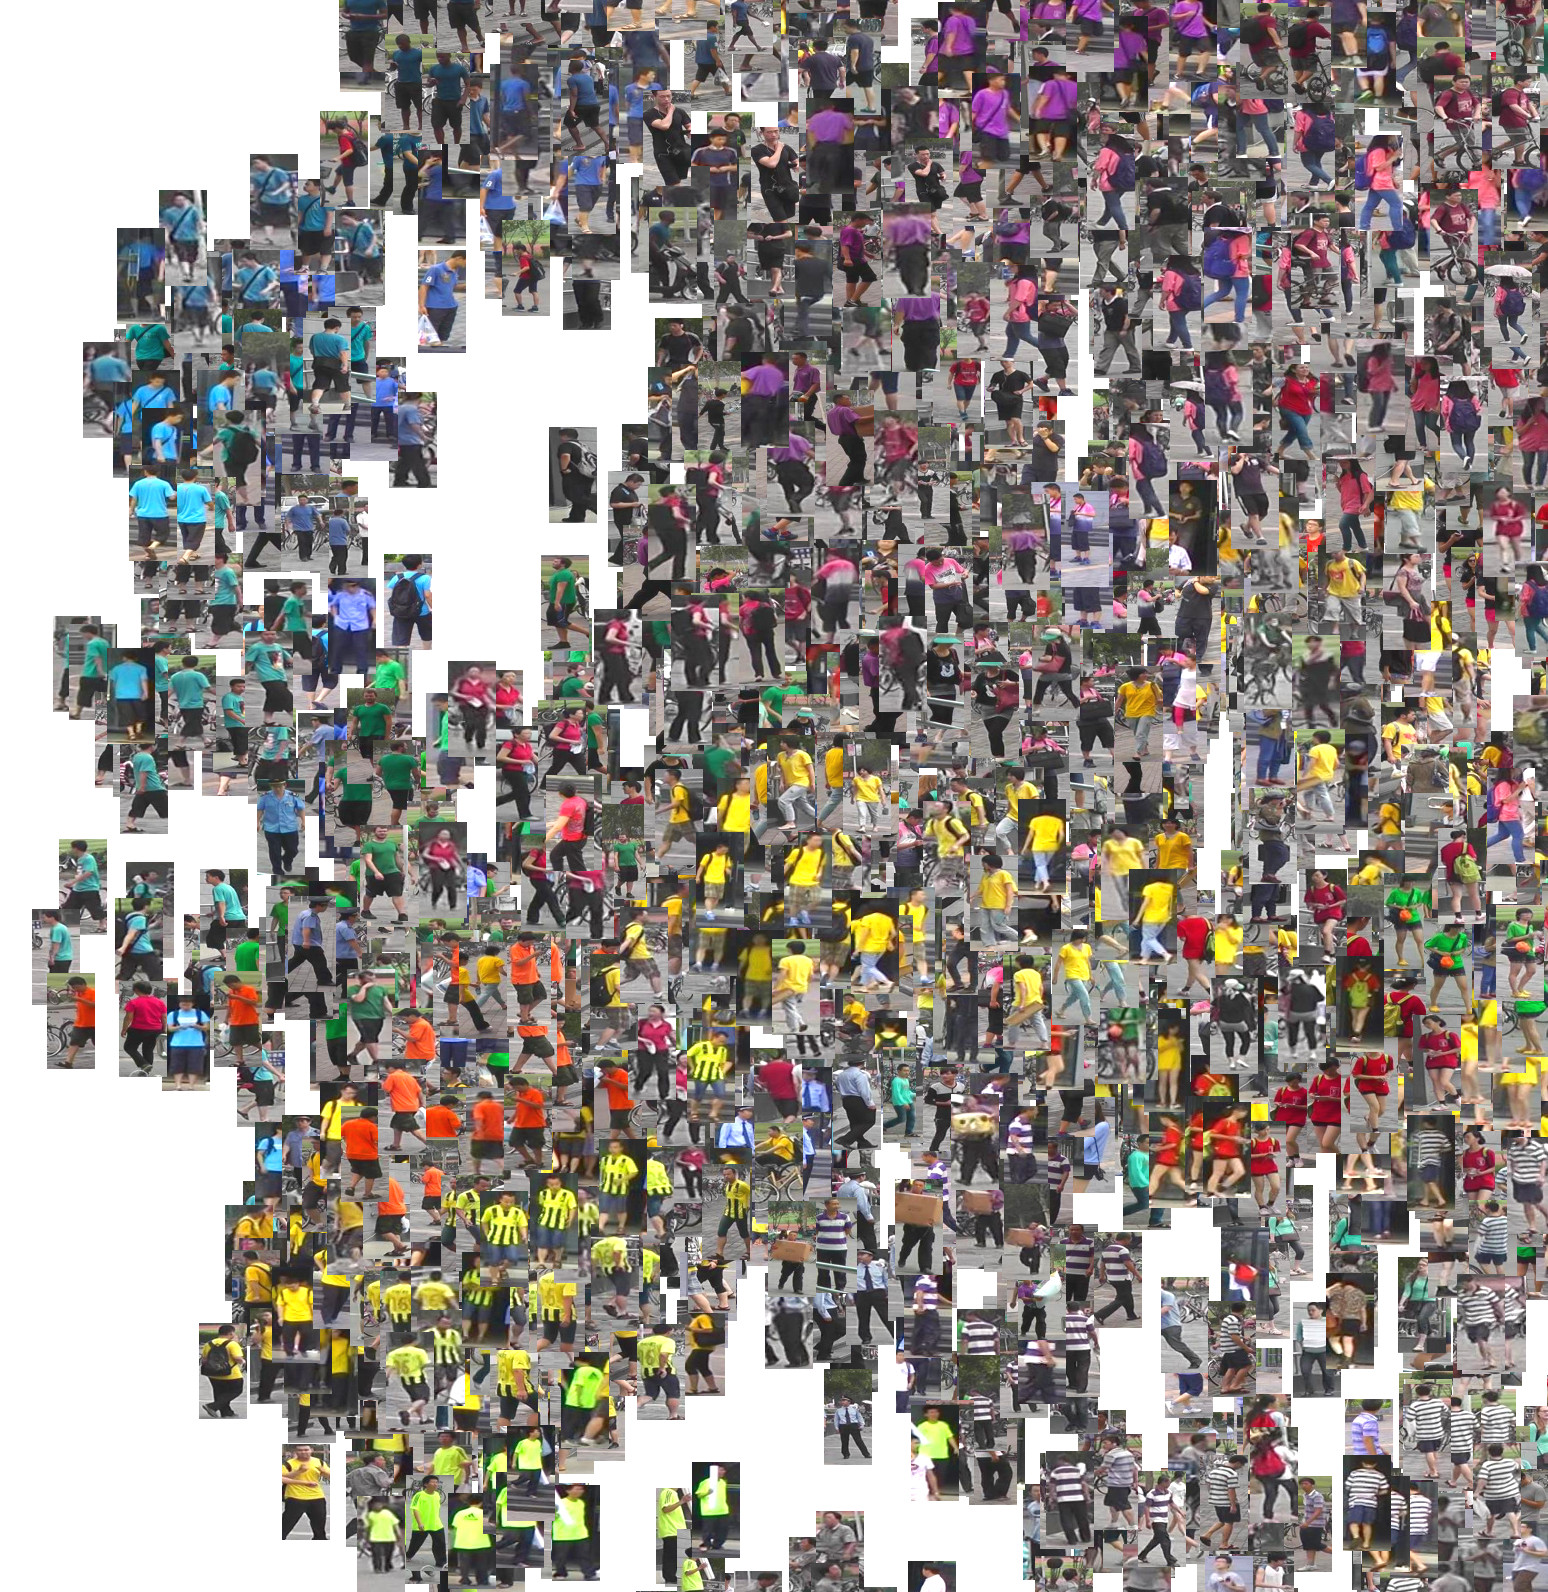
\includegraphics[width=0.6\textwidth]{informatica/embedding_paper_principal}
        \caption{Se representa una porción del \textit{dataset} \textit{Market-1501} tras aplicar el \textit{embedding} aprendido y posteriormente \textit{t-SNE}. Imagen extraída de \cite{informatica:principal}}
    \end{figure}

    Por ejemplo, un modelo que quiera resolver esta tarea podría aprender a mapear personas con exactamente la misma ropa a puntos cercanos.
\end{ejemplo}

\begin{ejemplo}

    Y para finalizar, consideremos nuestra tarea en concreto. Buscamos que las imágenes de la misma persona, aunque hayan pasado los años, se transformen en vectores cercanos. Y al contrario, que imágenes de dos personas distintas estén lo más lejos posible.

    Esto es especialmente complicado, como ya hemos comentando en \sectionref{ich:descrp_problema}, porque por ejemplo, nuestro modelo debe ver como más cercanos imágenes de un niño y un adulto con barba (ambos siendo la misma persona) que dos imágenes de dos adultos con barba (siendo distintas personas). Este problema en concreto lo hemos mostrado en la \imgref{img:messi_distintos_otro_adulto}
\end{ejemplo}


\subsection{\textit{Triplet Loss} como función de pérdida para aprender el \textit{embedding}} \label{isec:triplet_loss}

Ya sabemos que para resolver nuestro problema queremos que un modelo convolucional profundo aprenda un \textit{embedding} semántico que codifique la identidad de las personas independientemente de cambios en la edad. Lo que nos falta es una función de pérdida que optimice los parámetros de nuestro modelo. Justificaremos ahora el uso de \textit{triplet loss} como función de pérdida. Recordemos que estamos trabajando con funciones de la forma:

\begin{equation}
\begin{split}
    f_{\theta}: X & \to \R^N \\
    x & \mapsto f_{\theta}(x)
\end{split}
\end{equation}

y con una función de distancia:

\begin{equation}
\begin{split}
    D: X \times X & \to [0, \infty) \\
    x, y & \mapsto D(x, y)
\end{split}
\end{equation}

Para ser más concisos, usaremos la notación $D_{i, j} := D(f_{\theta}(x_i), f_{\theta}(x_j))$. Como su nombre indica, \textit{triplet loss} trabajará sobre triples. Esto es:

\begin{enumerate}
    \item Una imagen de un individuo concreto, a la que llamaremos \textbf{\textit{anchor}} o ancla
    \item Otra imagen distinta, pero del mismo individuo, a la que llamaremos \textbf{positiva}
    \item Una imagen de un individuo distinto, a la que llamaremos \textbf{negativa}
\end{enumerate}

En este caso, queremos que la distancia entre el \textit{embedding} del ancla y el \textit{embedding} de la positiva (que podemos denotar como $D_{A, P}$) sea mucho menor que la distancia entre el \textit{embedding} del ancla y el \textit{embedding} de la negativa (denotamos $D_{A, N}$). Por tanto, lo que realmente queremos es que:

\begin{equation}
    D_{A, P} \leq D_{A, N}
\end{equation}

o lo que es lo mismo,

\begin{equation}
    D_{A, P} - D_{A, N} \leq 0
\end{equation}

Una forma trivial de hacer que esa ecuación se cumpla, es haciendo que

\begin{equation}
    f(x) = \vec{0}; \dspace \forall x \in X
\end{equation}

con lo que obtendríamos un modelo totalmente inservible. Para evitar eso, introducimos un término $\alpha > 0$ que se conoce como \textbf{margen}, llegando a:

\begin{equation}
    D_{A, P} - D_{A, N} + \alpha \leq 0
\end{equation}

Buscamos que el término de la izquierda sea lo más negativo posible, por lo buscamos minimizar la siguiente función de pérdida:

\begin{equation} \label{ieq:triplet_loss_single_entry}
\begin{split}
    \mathcal{L}_{tri}(\theta; A, P, N) & := max \{D_{A, P} - D_{A, N} + \alpha, 0 \} \\
    &= ReLU(D_{A, P} - D_{A, N} + \alpha)
\end{split}
\end{equation}

Minimizando esta función de pérdida, lo que haremos será atraer elementos de la misma clase entre sí, y alejar elementos de clases distintas. Este proceso se refleja en la siguiente imagen:

\begin{figure}[H]
    \centering
    \includegraphics[width=1.0\textwidth]{informatica/triplet_loss_learning}
    \caption{Ejemplo gráfico del proceso de aprendizaje deseado con \textit{triplet loss}. Imagen creada a partir de datos de \cite{informatica:cacd_dataset} en base a \cite{informatica:facenet}}
\end{figure}

Notar que en \eqref{ieq:triplet_loss_single_entry} trabajamos con una sola entrada de tres datos en forma de imagen. A diferencia de un \textit{dataset} con datos etiquetados clásico, de la forma \lstinline{(entrada, valor de etiqueta)}, tenemos datos de la forma \lstinline{(imagen, identificador de individuo, edad)}. Esto supone un \textbf{problema} a resolver: cómo generamos \textit{batches} con triples de la forma \lstinline{(ancla, positivo, negativo)} para poder aplicar \eqref{ieq:triplet_loss_single_entry}. Explicaremos cómo solucionar esto en \sectionref{isubs:enfoque_offline_minado_triples}

Pero ahora veamos las \textbf{ventajas} que plantea este enfoque. La principal es que, a diferencia de otros enfoques basados en usar funciones de pérdida auxiliares (y que suelen forzar que la red solo pueda funcionar comparando pares de imágenes), el cómputo del \textit{embedding} es directo usando esta función de pérdida (\textit{end to end learning}). Optimizamos directamente la propiedad semántica del \textit{embedding} que deseamos obtener. Una vez entrenado el modelo es directo adaptar el modelo a tareas de \textit{clustering}, \textit{retrieval}, verificación, \ldots \cite{informatica:principal}. En \customref{isubs:impl_retr_adapter} mostramos lo sencillo que es realizar esta adaptación.

\subsubsection{Minado de triples \textit{offline}} \label{isubs:enfoque_offline_minado_triples}

Como ya hemos comentado, la tarea que debemos resolver ahora es la de generación de \textit{batches} adecuados para poder emplear \eqref{ieq:triplet_loss_single_entry} como función de pérdida a minimizar.

Por tanto, dado un conjunto de datos de la forma \lstinline{(imagen, identificador, edad)}, debemos obtener un conjunto de datos de la forma \lstinline{(img. ancla, img. positivo, img. negativo)}. Este último conjunto de datos puede ser una lista de triples o un conjunto de \textit{batches}. Como buscamos trabajar con \textit{batches}, en el caso de tener una lista de triples, podemos simplemente muestrear aleatoriamente y sin remplazo de dicha lista, repitiendo el muestreo tras cada época completada.

El \textbf{minado de triples \textit{offile}} es el enfoque clásico que se ha venido usando previo a \cite{informatica:facenet}, trabajo que introduce un enfoque \textit{online} que luego otros trabajos como \cite{informatica:principal} han ido mejorando. Para entender este minado veamos el ciclo de aprendizaje, que se divide en \textbf{varios pasos}.

En primer lugar, se realiza el minado \textit{offline} de los triples. Es decir, se obtiene una primera lista o conjunto de \textit{batches} de la forma \lstinline{(img. ancla, img.positivo, img.negativo)}. Una forma de hacer esto sería, por ejemplo, generar los triples de forma aleatoria, generar todos los posibles triples, $\ldots\dspace$ Aunque estas ideas no suelen funcionar en la práctica. Otra forma más efectiva es seleccionar los triples en base a algún estudio estadístico. O usar la red que vamos a optimizar para identificar aquellos triples en los que tiene más dificultad.

En segundo lugar, realizamos el aprendizaje sobre dicho conjunto de triples. En algunos casos, realizamos el entrenamiento completo sobre dicho conjunto inicial. En otros casos, principalmente cuando usamos la red para el minado de triples, pasadas algunas épocas de entrenamiento volvemos a generar otra vez la lista de triples. Así, triples que antes la red no identificaba propiamente, ahora sí que los identifica (\entrecomillado{network snapshots}, \cite{informatica:facenet}) y podemos buscar triples más interesantes.

Una vez computado una lista de triples $(a, p, n) \in \Omega$, la función de pérdida \eqref{ieq:triplet_loss_single_entry} se implementa de forma natural como en cualquier otro ámbito de \textit{batching}:

\begin{equation}
    \mathcal{L}_{tri}^{offline}(\theta; \Omega) := \frac{1}{\#\Omega} \sum_{(a, p, n) \in \Omega} \mathcal{L}_{tri}(\theta; a, p, n)
\end{equation}

En la literatura sobre aprendizaje automático normalmente se ignora el término $\frac{1}{\#\Omega}$ y se supone que siempre estamos dividiendo por el número de sumandos, con lo que nuestra función de error suele escribirse como:

\begin{equation}
    \mathcal{L}_{tri}^{offline}(\theta; \Omega) := \sum_{(a, p, n) \in \Omega} \mathcal{L}_{tri}(\theta; a, p, n)
\end{equation}

\subsubsection{Problemas del minado \textit{offline}}

El minado de triples \textit{offline} supone una serie de \textbf{problemas}:

\begin{itemize}
    \item Estamos dividiendo el proceso de aprendizaje en dos etapas, la de minado de triples y la de aprendizaje sobre estos triples. Esto añade complejidad a nuestra \textit{pipeline} (véase \customref{isec:pipeline})
    \item La adecuada elección de triples es fundamental. Si elegimos triples demasiado fáciles, la red no aprenderá nada nuevo, pues es muy fácil distinguir los ejemplos presentados. Sin embargo, si solo mostramos triples complicados, el modelo se centrará en aprender ejemplos extraordinarios y no sabrá distinguir el grueso de ejemplos más sencillos
        \begin{itemize}
            \item Además, generalmente los modelos aprenden rápidamente a distinguir la mayoría de ejemplos en los que las diferencias son relativamente evidentes. Por tanto, en pocas iteraciones la mayoría de triples generados de forma \textit{offline} son demasiado sencillos, lo que agrava mucho el problema que hemos comentado
        \end{itemize}
    \item Sería conveniente disponer de alguna forma de ajustar la complejidad de los triples presentados. Podemos confiar en que al ir re-generando la lista de triples, la complejidad vaya aumentando. Pero el algoritmo de minado debería tener alguna forma de controlar el énfasis que se hace en la búsqueda de combinaciones difíciles, lo que añade aún más complejidad al sistema
    \item El minado supone realizar un proceso de búsqueda, que es \textbf{muy lento} (evaluar de alguna forma todos los posibles triples supondría al menos $O(n^3)$). Lo ideal sería disponer de algún método que se basará en muestrear aleatoriamente de nuestra lista de elementos de la forma \lstinline{(imagen, identidad, edad)} (proceso que es muy rápido) y generar triples interesantes sobre dicho muestreo. Esto motiva la técnica introducida en \sectionref{isubs:triples_online}
\end{itemize}

\section{Mejoras técnicas objeto de estudio}

Hemos introducido todos los conceptos teóricos suficientes para plantear una solución basada en aprendizaje automático para nuestro problema. Sin embargo, una \textbf{parte fundamental de este trabajo consiste en explorar algunas mejoras técnicas} introducidas en \cite{informatica:principal}. Dichas mejoras se resumen en:

\begin{itemize}
    \item Introducir una técnica para minar de forma \textit{online} los triples, basada en el muestreo \textit{PK-Sampling}
    \item A partir del nuevo muestreo podemos definir dos variaciones sobre la función de pérdida
    \item Exploramos el uso de una nueva función de distancia
\end{itemize}

\subsection{Enfoque online de \textit{Triplet Loss}} \label{isubs:triples_online}

Buscamos modificar el minado de triples \textit{offline} para solucionar alguno de sus problemas que hemos comentado. Para ello implementaremos el siguiente proceso. En primer lugar, realizaremos un muestreo aleatorio sobre nuestros datos de la forma \lstinline{(imagen, identidad, edad)}. Este muestreo es rápido y no supone prácticamente tiempo de cómputo. Usando únicamente los datos de ese muestreo, generaremos triples y computaremos la función de pérdida apoyándonos en \eqref{ieq:triplet_loss_single_entry}. Dicha generación ya sí que supone un tiempo de cómputo considerable. Repetimos este proceso hasta agotar todos las entradas de nuestro \textit{dataset}, completando así una época de entrenamiento.

Ya podemos ver algunas \textbf{ventajas de este método}, incluso antes de haber especificado las dos partes fundamentales del proceso (muestreo y selección de triples):

\begin{enumerate}
    \item La ventaja más obvia es que, suponiendo que el tamaño de la muestra es significativamente mucho más pequeño que el tamaño de todo el conjunto de datos, la generación de triples consumirá potencialmente menos tiempo y será más efectiva
        \begin{itemize}
            \item Para afirmar esto rotundamente, tendríamos que realizar un estudio del tiempo del minado \textit{offline} en contraste a la suma de todos los tiempos de minado en cada muestreo
            \item Sin embargo, el tiempo usado es más eficiente, porque en cada muestreo estamos usando la red actualizada. En el minado \textit{offline} podemos gastar muchísimo tiempo en encontrar triples difíciles que, tras entrenar en unos pocos triples previos, acaben siendo sencillos. Por tanto, cuando la red vea triples algo avanzados en la lista, estos ya serán totalmente inútiles
        \end{itemize}
    \item Se facilita en gran parte el ajuste de la dificultad. Podemos buscar triples realmente difíciles, pero como solo se tiene acceso a una pequeña muestra, estamos controlando la dificultad. Así que podemos variar el tamaño de las muestras para buscar un punto medio entre ejemplos muy difíciles o ejemplos demasiado sencillos. Y todo esto sin contar con el factor de que vamos a usar la red actualizada para la elección de los triples
\end{enumerate}

Desarrollada esta visión de forma general, veamos cómo se implementa cada una de las partes, siguiendo las técnicas introducidas en \cite{informatica:principal}.

\subsection{Generación online de \textit{batches} usando \textit{P-K sampling}} \label{isubs:muestreo_datos_pk_sampling_teoria}

La \textbf{idea principal del muestreo} es lo que definiremos como \textbf{\textit{P-K sampling}}. Como ya hemos comentado en \sectionref{isubs:triples_online}, nuestra tarea ahora es generar un \textit{batch} de elementos de la forma \lstinline{(imagen, identidad, edad)}. En una segunda etapa (véase \sectionref{isubs:seleccion_de_triples}), otro algoritmo decide cómo generar triples a partir de estos datos.

El algoritmo de muestreo \textit{P-K sampling} es muy sencillo. En cada muestreo, seleccionamos aleatoriamente $P$ identidades de individuos (o clases, en un ambiente más general en el que no necesariamente estemos trabajando con imágenes de personas). Por cada una de las identidades, seleccionamos aleatoriamente $K$ imágenes asociadas a esa identidad. Por tanto, obtenemos una lista de $P \cdot K$ imágenes, a la que llamaremos \textbf{\textit{P-K batch}}. Para poder obtener triples interesantes en la siguiente etapa, parece que lo deseable es que ambos muestreos aleatorios sean sin repetición.

El hecho de tener $K$ imágenes por cada uno de los individuos seleccionados es lo que va a permitir al algoritmo de generación de triples obtener rápidamente triples interesantes.

\begin{figure}[H]
    \centering
    \includegraphics[width=0.6\textwidth]{informatica/ejemplo_grafico_pk_sampling}
    \caption{Ejemplo gráfico del proceso de \textit{P-K sampling}. Imagen extraída de \cite{informatica:paper_image_pk_sampling}}
\end{figure}

Queda aquí claro el \textbf{problema principal} que introduce esta técnica: si queremos muestrear $K$ imágenes de cada individuo sin repetición, cada individuo debe tener asociadas al menos $K$ imágenes. Así que a la hora de trabajar con un \textit{dataset}, siempre deberíamos comprobar la distribución del número de imágenes por individuo, como haremos en \sectionref{isec:base_datos_usada}.

\subsection{Selección de triples y variaciones en la función de pérdida} \label{isubs:seleccion_de_triples}

Una vez que tenemos un \textit{batch} de $P \cdot K$ elementos, deberemos generar una lista de triples en base a este \textit{batch}. Una vez se especifica cómo se seleccionan los triples, usando \eqref{ieq:triplet_loss_single_entry}, inducimos de forma natural y directa una cierta función de pérdida que actúa sobre estos \textit{P-K batches}.

Introducimos una notación que nos va a ser útil. Trabajamos $P \cdot K$ elementos, cada uno correspondiendo a una clase en concreto. Por tanto, indexaremos los elementos de la forma $x_k^p$ donde $p$ marca el identificador del individuo, y $k$ marca a cuál de las $K$ imágenes del individuo $p$ nos estamos refiriendo

\subsubsection{\textit{Batch Hard}} \label{isubsubs:batch_hard}

La primera idea es iterar sobre todos los elementos del \textit{P-K batch}, obteniendo así $P \cdot K$ anclas. Por cada ancla, seleccionamos el positivo y negativo \textbf{más complicado dentro de \textit{P-K batch}}. Por tanto, queda claro que \textbf{estamos usando la red para seleccionar triples difíciles} en cada \textit{batch} generado.

Esto introduce la siguiente función de pérdida, a la que llamaremos \textbf{\textit{Batch Hard}}:

\begin{equation}
    \mathcal{L}_{BH}(\theta, \hat{\Omega}) := \comentarencima{\sum_{p = 1}^P \sum_{k = 1}^K}{\text{todas las anclas}} [
        \comentarencima{\max_{k' = 1, \ldots, K} D(f_{\theta}(x_k^p), f_{\theta}(x_{k'}^p))}{\text{positivo más complicado}}
        - \comentarencima{\min_{\substack{p' = 1, \ldots, P \\ p' \neq p \\ k' = 1, \ldots, K}} D(f_{\theta}(x_k^p), f_{\theta}(x_{k'}^{p'}))}{\text{negativo más complicado}}
        + \alpha]_+
\end{equation}

donde $[x]_+ := max \{0, x\} = ReLU(x)$ y $\hat{\Omega}$ se refiere a un \textit{P-K batch}. No olvidemos que no estamos escribiendo la división por el número de sumandos, $P \cdot K$.

Estamos generando \textbf{triples moderados}, porque estamos buscando los triples más difíciles, pero dentro de un \textit{batch} relativamente pequeño comparado a el total del conjunto de datos. Con esto estamos ajustando la dificultad de los triples cómodamente, resolviendo el problema que comentábamos en \sectionref{isubs:enfoque_offline_minado_triples}. Aumentando el valor de $\{P, K\}$ aumentamos el tamaño del espacio de búsqueda, y por tanto podremos encontrar triples mucho más difíciles. Sin embargo, hay que tener siempre en cuenta el coste en tiempo de cómputo.

Queda claro que, gracias al proceso de \textit{P-K sampling}, ahora es factible realizar una búsqueda de triples interesantes en profundidad, basándonos en el estado más actualizado de la red para calcular la dificultad de los triples. Esta búsqueda extensiva no habría sido posible si la planteásemos sobre todo el conjunto de datos.

\subsubsection{\textit{Batch All}} \label{isubsubs:batch_all}

Motivados por lo que acabamos de comentar en \sectionref{isubsubs:batch_hard}, podemos plantearnos usar todos los posibles triples dentro de un \textit{P-K batch} como un enfoque que ahora cobra más sentido (ya hemos comentado en \sectionref{isubs:enfoque_offline_minado_triples} que realizar esto sobre todo el conjunto de datos no parece una buena idea).

Realizar esto introduce la función de pérdida que llamaremos \textbf{\textit{Batch All}}:

\begin{equation} \label{ieq:batch_all}
    \mathcal{L}_{BA}(\theta; \hat{\Omega}) :=
    \comentarencima{\sum_{p = 1}^{P} \sum_{k = 1}^K}{\text{todas anclas}}
    \comentardebajo{\sum_{\substack{k' = 1 \\ k' \neq k}}^{K}}{\text{todas pos.}}
    \comentarencima{\sum_{\substack{p' = 1 \\ p' \neq p}}^P \sum_{n = 1}^K}{\text{todas neg.}} \dspace[
        D(f_{\theta}(x_k^p),f_{\theta}(x_{k'}^p)) - D(f_{\theta}(x_k^p),f_{\theta}(x_{n}^{p'})) + \alpha
    ]_+
\end{equation}

Está claro que, por el número de sumandos, esta aproximación es viable gracias a que nuestro \textit{P-K sampling} reduce mucho el número de elementos sobre los que operamos. Dicho número de sumandos viene dado por:

\begin{equation}
    P \cdot K \cdot (K - 1) \cdot (P - 1) \cdot K = P^2 - P + K^3 - K^2 \approx P^2 + K^3
\end{equation}

Esta aproximación sería completamente inviable sobre un número muy elevado de elementos. Pensemos, por ejemplo, en las 163446 imágenes de \textit{CACD} (conjunto de datos que estudiamos en \sectionref{isec:dataset_cacd}).

\subsubsection{Mejoras introducidas a partir de la experimentación} \label{isubsubs:mejoras_sumandos_no_nulos}

En \cite{informatica:principal}, a raíz de observar los resultados de la experimentación, señalan algunos puntos débiles en las dos funciones de pérdida que introducen a partir del \textit{P-K sampling}.

Principalmente, en \customref{isubsubs:batch_all}, podemos ver un posible fallo en la función de pérdida \eqref{ieq:batch_all}. Si se da el caso de que la mayoría de triples generados son fáciles (hecho muy probable al estar generando todas las combinaciones de triples), los escasos triples que realmente son difíciles se desvanecerán. Esto porque la mayoría de términos serán cero (al estar aplicando $[x]_+$). Y los pocos términos que no son cero, se dividen por el número total de elementos, que ya hemos visto que es elevado.

Por tanto, una mejora sencilla a esta función de pérdida es dividir únicamente por el número de sumandos no nulos. A estos sumandos no nulos también se les llama sumandos activos \cite{informatica:principal}. Esta mejora la podemos aplicar también a \textit{batch hard}, obteniendo dos nuevas funciones de pérdida, a las que denotaremos por $\mathcal{L}_{BA \neq 0}$ y $\mathcal{L}_{BH \neq 0}$.

\subsubsection{Algunas observaciones y conclusiones} \label{isubsubs:observaciones_conclusiones_pksampling}

En primer lugar, cabe destacar que, como señalan \cite{informatica:principal}, las dos nuevas funciones de pérdida introducidas equivalen al planteamiento clásico de \textit{triplet loss} si entrenásemos indefinidamente.

El desarrollo que hemos realizado justifica las siguientes \textbf{ventajas} de los nuevos métodos:

\begin{itemize}
    \item El uso del \textit{P-K sampling} y las dos nuevas funciones de pérdida (con las variantes técnicas que consideran los sumandos activos) permite realizar un aprendizaje \textit{end-to-end}, sin añadir un paso adicional en el bucle de aprendizaje, evitando así la gran complejidad añadida del minado \textit{offline}
    \item Además, conseguimos un manejo preciso de la dificultad de los triples obtenidos. Controlando el valor de $\{P, K\}$, controlamos el espacio de búsqueda y, en definitiva, la dificultad. Todo esto de forma cómoda y sin introducir apenas complejidad en nuestro \textit{pipeline}
    \item Aunque no lo hemos comprobado, pensamos que esto acelera los tiempos de cómputo, al estar realizando el minado de triples sobre \textit{batches} de tamaño considerablemente reducidos
    \item Y aunque no mejorásemos el tiempo de computo, lo que sí sabemos que mejoramos es la eficacia del minado de triples. El minado de triples \textit{online} usa una red mucho más actualizada, para generar una lista mucho más pequeña que probablemente no se degrade tanto como la generada por un minado \textit{offline} sobre todo el conjunto de datos, mucho más grande
    \item Es más, estamos controlando el efecto de los triples demasiado sencillos, que no tendremos en cuenta a la hora de promediar en la función de pérdida
\end{itemize}

A pesar de esto, a raíz de trabajar con estas nuevas técnicas, identificamos los siguientes \textbf{inconvenientes}:

\begin{itemize}
    \item Introducimos dos hiperparámetros, $\{P, K\}$ que deberemos ajustar correctamente, pues tienen un enorme impacto en los resultados del proceso de entrenamiento. Por tanto, se hace fundamental tener un proceso de \textit{hyperparameter tuning} robusto, como introducimos en \sectionref{isec:hptuning_kfold_cross_validation} e implementamos en \sectionref{isec:hp_tuning}
    \item Tenemos que tener mucho cuidado con usar valores elevados de $\{P, K\}$ por dos motivos. El primero, y como ya hemos comentado, valores altos implicarán que los tiempos de cómputo para la generación de triples crecerán rápidamente. El segundo es que el tamaño de los \textit{batches} crecerán considerablemente, llegando a colapsar la memoria disponible de la \textit{GPU}
    \item Hemos comprobado en la práctica que es realmente fácil colapsar la memoria \textit{GPU}, usando modelos profundos como \textit{ResNet50} con valores de $P \cdot K = 100$. Esto supone que, aunque no estuviéramos limitados por el tiempo de cómputo, el colapso de la memoria limita el conjunto de valores $\{P, K\}$ con los que podemos experimentar
    \item Si queremos usar valores altos de $K$, nuestro \textit{dataset} lo debe permitir, teniendo una buena distribución de imágenes por individuo. Por este motivo hemos estudiado esta distribución en \sectionref{isec:base_datos_usada}. Se pueden explorar técnicas como el aumentado de datos para alcanzar el número de imágenes por individuo deseado, pero solo serán efectivas si dicha distribución es buena para empezar (véase \sectionref{isec:aumentado_datos})
    \item Tanto por el formato de los datos con los que hemos trabajado, como por el cambio fundamental realizado en el \textit{sampling} de los datos, hemos tenido que realizar un \textbf{esfuerzo considerable de implementación}, al no poder basarnos en la mayor parte de los casos en código implementado por alguna biblioteca de aprendizaje automático. Esto se ve reflejado en \sectionref{ich:implementacion}
\end{itemize}

\subsection{Variaciones en la función de distancia}

En todos los conceptos que hemos ido introduciendo la función de distancia

\begin{equation}
    D: X \times X \to [0, \infty)
\end{equation}

ha estado presente, pero todavía no hemos introducido ninguna función concreta. En el ambiente de \textit{AIFR} se suele usar la distancia euclídea al cuadrado, esto es:

\begin{equation}
    D(x_i, x_j) := ||f_{\theta}(x_i) - f_{\theta}(x_j)||^2_2
\end{equation}

Sin embargo, motivados por \cite{informatica:principal}, decidimos usar la distancia euclídea usual. En este trabajo se afirma que, en base a la experimentación, de esta forma se obtienen entrenamientos más estables. Además, usando la distancia euclídea usual, el margen es más fácil de interpretar, porque marca la diferencia de distancias, y no la diferencia de cuadrados de distancias. Por lo tanto, en base a dicho trabajo, decidimos tomar:

\begin{equation}
        D(x_i, x_j) := ||f_{\theta}(x_i) - f_{\theta}(x_j)||_2
\end{equation}

\subsection{Márgenes suaves} \label{isec:margenes_suaves}

En \sectionref{isec:triplet_loss} hemos justificado por qué es necesario introducir un término $\alpha$ para controlar el margen y evitar que nuestro modelo aprenda a colapsar todas las entradas al vector $\vec{0}$. Con esto llegamos a la ecuación \eqref{ieq:triplet_loss_single_entry}.

En dicha función de pérdida, el propósito de $x \mapsto \max\{0, x + \alpha\}$ (conocida comúnmente como \textit{hinge function}) es no corregir ejemplos que, en vista del margen $\alpha$ establecido, ya son correctos. Pero puede ser que estemos interesados en afinar aún más ejemplos que, para dicho valor del margen, sean correctos. Con esto conseguiríamos seguir acercando imágenes del mismo individuo lo máximo posible \cite{informatica:principal}. Es por esto que se propone en usar la función \textbf{\textit{softplus}}:

\begin{equation}
    x \mapsto ln(1 + exp(x))
\end{equation}

Dicha función puede verse como una versión suavizada de la función \textit{hinge}. Decae exponencialmente, por lo que ejemplos correctos se penalizarán exponencialmente menos cuanto más cercanos estén, pero contrasta con la función \textit{hinge} en que no presenta un salto o corte fuerte. Por tanto, se suele decir que estamos usando un \textbf{margen suave}. Además, una ventaja de esta función es que \textbf{desechamos el hiperparámetro $\alpha$}, el cual ya no tenemos que fijar a través de algún método (como podría ser el \textit{hyperparameter tuning}).

\begin{figure}[H]
\centering
    \begin{subfigure}{.5\textwidth}
        \centering
        \includegraphics[width=0.8\linewidth]{informatica/desmos_hinge}
        \caption{Función \textit{hinge} con $\alpha = 2$}
    \end{subfigure}%
    \begin{subfigure}{.5\textwidth}
        \centering
        \includegraphics[width=0.8\linewidth]{informatica/desmos_softplus}
        \caption{Función \textit{softplus}}
    \end{subfigure}

    \begin{subfigure}{.5\textwidth}
        \centering
        \includegraphics[width=0.8\linewidth]{informatica/desmos_conjunta}
        \caption{En azul, \textit{hinge} con $alpha = 0$. En rojo, \textit{softplus}}
    \end{subfigure}


\caption{Gráfica de las dos funciones para trabajar con los márgenes, y una gráfica conjunta que muestra su similitud}
    \label{img:graficas_margenes}
\end{figure}

Las gráficas mostradas en \imgref{img:graficas_margenes} nos sirven para visualizar de forma sencilla todo lo que hemos comentado. La función \textit{softplus} actúa como una \textit{hinge} suavizada. El hecho de que se parezcan tanto cuando hacemos que el margen de \textit{hinge} sea cero nos hace pensar que \textit{softplus} va a actuar como una \textit{hinge} en la que no hay margen, y por lo tanto, acercará elementos de la misma clase todo lo que pueda.

 % fundamentos teoricos
\chapter{Modelización de la tarea de aprendizaje} \label{ch:tarea_aprendizaje}

La tarea de aprendizaje que consideramos es la de clasificación. Durante todo el desarrollo, pensaremos en la \textbf{clasificación de imágenes}. En este caso, el enfoque que más éxito ha tenido históricamente es el uso de redes convolucionales profundas y, más actualmente, el uso del modelo \entrecomillado{transformer}.

Dado un elemento $X = (\nv{x_1}, \ldots, \nv{x_N})$, donde $\nv{x_i} \in \R^s \ \forall i \in \deltaset{N}$, queremos clasificarlo en alguna de las etiquetas $\mathcal{Y} = \{1, \ldots, Y \} = \deltaset{Y}$.

Con esto, podemos ver que los datos de entrada viven en el espacio

$$\mathcal{X} := \R^s \times \overset{N}{\ldots} \times \R^s = (R^s)^N$$

Esta representación de los datos de entrada es natural en muchas situaciones. En el caso de las imágenes, podemos considerar cada vector $\nv{x_i}$ como un conjunto de \textit{pixels} de la imagen. Idealmente, cada vector de \textit{pixels} debería contener un vecindario de \textit{pixels}, es decir, \textit{pixels} adyacentes. Podemos incluso considerar \textit{pixels} que aparezcan en más de un vector. Por ejemplo, podemos considerar $\nv{x_i}$ como la fila o columna $i$-ésima de la imagen.

Por ejemplo, el trabajo que presenta el conocido modelo  de deep learning \textit{VIT} propone una arquitectura \entrecomillado{transformer} a la que que se le pasa \entrecomillado{patches} de la imagen para poder explotar el mecanismo de atención: \entrecomillado{we split an image into patches and provide the sequence of linear embeddings of these patches as an input to a Transformer} \footnote{\cite{matematicas:vit}}
\todo{No sé si así está bien referenciado el trabajo al que me refiero}

Para decidir la etiqueta de un elemento, consideramos $Y$ \textbf{funciones de puntuación}:

$$\{h_y: \mathcal{X} \to \R \dspace / \dspace y \in \mathcal{Y} \}$$

Con esto, dado un elemento $X \in \mathcal{X}$, lo clasificaremos buscando la etiqueta cuya función de puntuación sea máxima, es decir:

$$\hat{y} := \underset{y \in \mathcal{Y}}{argmax} \dspace h_y(X)$$

Por tanto, nuestro \textbf{espacio de hipótesis} $\Gamma$ es el conjunto de funciones $\mathcal{X} \to \R$. Tanto en la práctica con modelos de \textit{machine learning}, como en nuestras dos modelizaciones, trabajamos en un subconjunto $\tilde{\Gamma} \subset \Gamma$ de funciones de puntuación, implementables o bien por el modelo de \textit{machine learning} o bien por nuestra modelización teórica.

\section{Espacio de hipótesis general}

\subsection{Justificación para la representación de las funciones de puntuación} \label{sec:justificacion_func_repr}

\todo{Desarrollar el apéndice 6 donde se justifica que esta ecuación es lo suficientemente general}

\subsection{Representación de las funciones de puntuación} \label{sec:repr_funciones_puntuacion}

Por todo esto, las funciones de puntuación vendrán dadas de la forma:

\begin{equation} \label{eq:puntuacion_general}
    h_y(\nv{x_1}, \ldots, \nv{x_N}) = \sum_{d_1, \ldots, d_N = 1}^{M} \mathcal{A}^y_{d_1, \ldots, d_N} \prod_{i = 1}^N f_{\theta_{d_i}}(\nv{x_i})
\end{equation}

Explicamos ahora algunos detalles sobre esta ecuación, que será central en nuestro trabajo.

En primer lugar, usamos la notación $\sum_{d_1, \ldots, d_N = 1}^{M}$ para denotar $\sum_{d_1 = 1}^{M} \sum_{d_2 = 1}^{M} \ldots \sum_{d_N = 1}^{M}$

Las funciones $f_{\theta_1}, \ldots, f_{\theta_M}: \R^s \to \R$ son las \textbf{funciones de representación}. Cada una de estas funciones se selecciona de una familia paramétrica

$$\mathcal{F} = \{ f_{\theta}: \R^s \to \R / \theta \in \Theta \}$$

Algunas funciones de representación usuales son:

\begin{itemize}
    \item \textit{Wavelets}
    \item Funciones de base radial (\textit{RBF}), normalmente la Gaussiana
    \item Neuronas
\end{itemize}

El tensor $\mathcal{A}^y$ será el \textbf{tensor de coeficientes}. Por la sumatoria en \eqref{eq:puntuacion_general}, es claro que tiene orden $N$ y dimensión $M$ en cada modo. Es decir, $\mathcal{A} \in \espaciotensores{N}{M}$.

La tarea de aprendizaje ahora será aprender los valores de los parámetros $\theta_1, \ldots, \theta_M$ y los valores de los tensores de coeficientes $\mathcal{A}^1, \ldots, \mathcal{A}^Y$.

\begin{observacion}

    Estamos usando las mismas funciones de representación $f_{\theta_1}, \ldots, f_{\theta_M}: \R^s \to \R$ para todas las funciones de representación $h_y, y \in \mathcal{Y}$, lo único que cambia entre las distintas funciones de puntuación es el tensor de coeficientes $\mathcal{A}^y$.


    Notar además que en la ecuación \refeq{eq:puntuacion_general}, los vectores de entrada $\nv{x_i}$ solo participan en el productorio que involucra computar $f_{\theta_{d_i}}(\mathbf{x_i})$.

    Por tanto, aunque esto se corresponda más con el posterior diseño de las redes neuronales que vamos a realizar, podemos considerar como paso inicial, compartido en los dos modelos que proponemos, el cómputo de los valores:

    $$\{f_{\theta_d}(\nv{x_i}) / d \in \deltaset{M},\ i \in \deltaset{N} \}$$

    Una vez que hayamos computado esos $M \cdot N$ valores, ya no necesitamos los valores $\nv{x_i}$ para nada más. Con esto, es natural considerar que nuestro modelo tenga una primera capa que compute esos valores. Podemos considerar dicha capa como una \textbf{primera capa convolucional} con $M$ canales, a la que llamaremos \textbf{capa de representación}.

    Y como ya hemos comentado, estamos usando las mismas funciones de representación para las $Y$ funciones de puntuación. Por tanto, fijados los parámetros $\theta_i$, en todas las funciones de puntuación la capa de representación será la misma.
\end{observacion}

\begin{observacion}
    Sabemos, por lo comentado en \customref{sec:justificacion_func_repr}, que al trabajar con \textit{wavelets}, \textit{RBFs} y neuronas, podemos extraer un conjunto numerable de funciones que sea total y linealmente independiente. También gracias a \customref{sec:justificacion_func_repr}, que por tanto el siguiente espacio de funciones es total y linealmente independiente:
    \todo{Tengo que mirar esto bien. Creo que aquí es cuando discuten el valor de $M$ para saber que me vale con un subconjunto finito de funciones de representación. \textbf{MIRAR BIEN}}

    $$\{(\nv{x_1}, \ldots, \nv{x_N}) \mapsto \prod_{i = 1}^{N} f_{\theta_{d_i}} (\nv{x_i}) \dspace / \dspace d_i \in \deltaset{M} \dspace \forall i \in \deltaset{N}\}$$

    Por tanto, actúa de forma parecida a una base de un espacio vectorial. Teniendo en cuenta este comportamiento similar, podemos pensar que el tensor $\mathcal{A}^y$ nos da los coeficientes de la función de puntuación $h_y$ en dicha \entrecomillado{base}.

    \todo{Tengo que desarrollar bien esa sección para justificar todas estas cosas que estoy diciendo}
\end{observacion}

\begin{observacion}
    Como ya sabemos, como $\mathcal{A} \in \espaciotensores{N}{M}$, tenemos que optimizar el valor de $M^N$ valores reales a través del proceso de aprendizaje. Esto supone un reto, que \textbf{motiva el uso de los dos modelos}, que se basarán en descomposiciones tensoriales para que el aprendizaje del tensor de coeficientes sea más factible.
    \todo{Tengo que comentar en la introducción que el número de elementos de un tensor N, M es M elevado a N}
\end{observacion}

\endinput
 % estado del arte
\chapter{Modelización de las redes neuronales} \label{ch:modelizacion}

A partir de las herramientas matemáticas que hemos introducido en \customref{ch:matematicas_fundamentales} y de la modelización de la tarea de aprendizaje realizada en \customref{ch:tarea_aprendizaje}, buscamos desarrollar una modelización matemática de las redes neuronales con las que se suele trabajar en la práctica. Para que sea una \textbf{buena modelización}, esta debería cumplir que:

\begin{itemize}
	\item Sea lo más parecida a los modelos que se usan en la práctica.
	\item Permita obtener resultados interesantes.
\end{itemize}

Usando descomposiciones tensoriales, modelaremos dos tipos de redes:

\begin{itemize}
	\item Redes neuronales no profundas, a partir de la descomposición \textit{CANDECOMP/PARAFAC} o descomposición \textit{CP}.
	\item Redes convolucionales profundas, a partir de la descomposición jerárquica de \textit{Tucker} o descomposición \textit{HT} por sus siglas en inglés.
\end{itemize}

Las \textbf{modelizaciones son muy cercanas a las arquitecturas usadas en la práctica del aprendizaje automático}. Principalmente, porque tienen en cuenta las tres propiedades características de una red convolucional:

\begin{enumerate}
	\item Localidad.
	\item Compartición de parámetros, que junto a la localidad, da lugar a la convolución.
	\item \textit{Pooling}.
\end{enumerate}
\todo{Desarrollar de forma más extensa qué significan estas propiedades. Antes digo que voy a explicar qué son estas propiedades. Y además, estoy repitiendo el listado, por lo que tengo que desarrollar bien estas propiedades}

\section{Modelo \textit{CP}}

Este modelo será el resultado de aplicar la descomposición tensorial \textit{CP} en la función de puntuación dada por \eqref{eq:puntuacion_general}. Como veremos más adelante, esto resultará en un modelo \textit{shallow}, con una única capa convolucional oculta.

\subsection{Descomposición CANDECOMP/PARAFAC} \label{subs:descomposcion_cp}

En esta sección introduciremos la descomposición tensorial \textit{CANDECOMP/PARAFAC}. Esta es la descomposición más sencilla de las dos descomposiciones que vamos a manejar. Empecemos introduciendo la siguiente propiedad sobre los tensores puros:

\begin{proposicion}[Rango matricial de los tensores puros]
	Sean $\nv{v} \in \R^{N}, \nv{w} \in \R^{M}$ dos vectores. Entonces su producto tensorial puede expresarse como:

	$$\nv{v} \otimes \nv{w} = \nv{v} \nv{w}^T \in \espaciomatrices{N}{M}$$

	Además, esta matriz es de rango uno o cero (este último caso ocurre únicamente cuando alguno de los dos vectores es $\vec{0}$)
\end{proposicion}

\begin{proof}

	Sean $\nv{v} = (v_1, \ldots, v_N)$ y $\nv{w} = (w_1, \ldots, w_M)$ dos vectores cualesquiera. Entonces, usando la expresión del producto tensorial que introducimos en \customref{sec:otra_forma_tensores}, tenemos que:

	\begin{equation}
		\nv{v} \otimes \nv{w} = (v_i w_j)_{i \in \deltaset{N},\ j \in \deltaset{M}}
	\end{equation}

	O lo que es lo mismo:

	\begin{equation}
		\nv{v} \otimes \nv{w} = \begin{pmatrix}
			v_1 w_1 & v_1 w_2 & \ldots & v_1 w_M \\
			v_2 w_1 & v_2 w_2 & \ldots & v_1 w_M \\
			\vdots  & \vdots  &        & \vdots  \\
			v_N w_1 & v_N w_2 & \ldots & v_N w_M \\
		\end{pmatrix}
	\end{equation}

	Que claramente se corresponde con la expresión de $\nv{v} \nv{w}^T$. Además, es claro que la fila $i$-ésima viene dada por el vector fila

	$$(v_i w_1, v_i w_2, \ldots, v_i w_M) = v_i (w_1, \ldots, w_M) = v_i \nv{w}^T$$

	Por tanto, todas las filas son combinación lineal de una de las filas.

	En el caso de que alguno de los dos vectores $\nv{v}$ o $\nv{w}$ sea $\vec{0}$, tenemos que la matriz $\nv{v} \otimes \nv{w}$ es la matriz de ceros, y por tanto su rango es cero.

	Estudiado ese caso, ahora podemos suponer que $\nv{v}, \nv{w} \neq \vec{0}$, y por tanto se debe cumplir que $\exists i_0 \in \deltaset{N}: v_{i_0} \neq 0$. Esa será la fila que escogemos para expresar el resto de filas como combinación lineal de esta, aprovechando de que es no nula. Dicha fila se puede expresar como $v_{i_0} \nv{w}^T$. La fila $i$-ésima se puede expresar como $v_i \nv{w}^T$. Y por tanto:

	\begin{equation}
		\begin{split}
			v_i \nv{w}^T = \lambda \cdot v_{i_0} \nv{w}^T \iif & \lambda = \frac{v_i}{v_{i_0}} \\
			& \lambda \neq 0 \iif v_i \neq 0
		\end{split}
	\end{equation}

	Con esto sabemos que $rank(\nv{v} \otimes \nv{w}) \leq 1$, pero podría darse el caso de que el rango fuese cero aún siendo $\nv{v}, \nv{w} \neq \vec{0}$. Sin embargo, esto no es posible. Como $\nv{v}, \nv{w} \neq \vec{0}$, entonces $\exists i_0 \in \deltaset{N}, \exists j_0 \in \deltaset{M}$ de modo que $v_{i_0}, w_{j_0} \neq 0$. Por tanto, el menor de orden 1 asociado a la fila $i_0$-ésima y columna $j_0$-ésima tiene el valor $v_{i_0} w_{j_0} \neq 0$, y con ello, $rank(\nv{v} \otimes \nv{w}) \geq 1$.

\end{proof}

\begin{observacion}
	Estamos escribiendo la igualdad $\nv{v} \otimes \nv{w} = \nv{v} \nv{w}^T$ sin definir lo que significa la igualdad entre un tensor de orden 2 y una matriz. Sin embargo, esta igualdad es totalmente natural. Decimos que un tensor de orden dos y una matriz son iguales cuando las dimensiones de la matriz y las dos dimensiones del tensor coinciden, y cuando las entradas de ambos coinciden.
\end{observacion}

La anterior proposición muestra que los tensores puros que vienen dados como producto tensorial de dos vectores tienen un rango matricial igual a uno (en caso de que no sean ambos vectores nulos). Es natural plantearse generalizar esta propiedad a tensores puros que vengan dados como producto tensorial de $N$ vectores. Pero de momento no tenemos una herramienta para comparar tensores de orden $N > 2$ con matrices. Esto motiva la introducción de la descomposición tensorial \textit{CANDECOMP/PARAFAC}:

\begin{proposicion}[\textbf{Descomposición \textit{CANDECOMP/PARAFAC}}]
	Todo tensor $\mathcal{A}$ puede ser expresado como la suma de tensores puros. Es decir, $\forall \mathcal{A} \in \R^{M_1 \times \cdots \times M_N}$, $\exists Z \in \N$:

	\begin{equation} \label{eq:cp_decomp}
		\mathcal{A} = \sum_{i = 1}^Z \nv{v_i^{(1)}} \otimes \cdots \otimes \nv{v_i^{(N)}};
		\qquad \nv{v_i^{(k)}} \in \R^{M_k},
		\dspace \forall i \in \deltaset{Z},
		\dspace \forall k \in \deltaset{N},
	\end{equation}
\end{proposicion}

\begin{observacion}[Origen del nombre de la descomposición]
	En 1927 Hitchcock propone la idea de expresar un tensor como la suma de tensores de rango uno. En 1970 se introducen dos trabajos independientes que resuelven esta tarea. El primero, introducido por Carol y Chang, propone la descomposición canónica (\textit{CANonical DECOMPosition} o \textit{CANDECOMP}). El segundo trabajo, introducido por Harshman, propone la descomposición por factores paralelos (\textit{PARallel FACtors} o \textit{PARAFAC}). Más tarde se descubre que ambas descomposiciones son equivalentes, por lo que se adopta el nombre conjunto \cite{matematicas:cp_nombre_paper}.
\end{observacion}

\begin{observacion}
	Esta descomposición es equivalente a la siguiente descomposición:

	\begin{equation}
		\mathcal{A} = \sum_{i = 1}^Z \lambda_i \cdot \nv{v_i^{(1)}} \otimes \cdots \otimes \nv{v_i^{(N)}};
		\qquad \nv{v_i^{(k)}} \in \R^{M_k},
		\dspace \lambda_i \in \R,
		\dspace \forall i \in \deltaset{Z},
		\dspace \forall k \in \deltaset{N},
		\dspace Z \in \N
	\end{equation}

	Puesto que podemos considerar:

	\begin{equation}
		\nv{w_i^{(1)}} := \lambda_i \cdot \nv{v_i^{(1)}} \in \R^{M_1}
	\end{equation}

	y usando de nuevo las propiedades del producto tensorial:

	\begin{equation}
		\lambda_i \cdot \nv{v_i^{(1)}} \otimes \nv{v_i^{(2)}} \otimes \cdots \otimes \nv{v_i^{(N)}} = \nv{w_i^{(1)}} \otimes \nv{v_i^{(2)}} \otimes \cdots \otimes  \nv{v_i^{(N)}}
	\end{equation}
\end{observacion}

\begin{observacion}
	Nótese que el número de vectores que multiplicamos tensorialmente es constante, no varía dicho número de vectores entre sumandos. Y dicho número coincide con el orden $N$ del tensor que estemos construyendo.
\end{observacion}

\begin{proof} \label{proof:demostracion_cp_es_universal}
	% TODO -- seguir por aqui
	Queremos descomponer el tensor $\mathcal{A}$ que tiene orden $N$ y dimensión $M_k$ en cada dimensión $k \in \deltaset{N}$. Por tanto, $\mathcal{A}$ tiene $M_1 \cdot M_2 \cdot \ldots \cdot M_N$ elementos. En base a esto, tomamos $Z = M_1 \cdot M_2 \cdot \ldots \cdot M_N$ y en cada sumando de la descomposición buscamos colocar un único coeficiente del tensor en su índice correspondiente.

	Por tanto, en cada sumando buscamos encontrar vectores cuyo producto tensorial genere un tensor, de dimensiones adecuadas, con todas las entradas nulas salvo la entrada de la que nos ocupamos en esa iteración.

	Para que la demostración sea más clara cambiaremos la forma de indexar la suma. En la proposición estamos usando un único índice que llega hasta $Z = M_1 \cdot \ldots \cdot M_N$. Esto es lo mismo que usar $N$ índices que lleguen hasta $M_k$, y así la sumatoria queda:

	\begin{equation}
		\mathcal{A} = \sum_{d_1 = 1}^{M_1} \sum_{d_2 = 1}^{M_2} \cdots \sum_{d_N = 1}^{M_N} \lambda_{i_1, \ldots, i_N} \cdot \nv{v_{(i_1, \ldots, i_N)}^{(1)}} \otimes \ldots \otimes \nv{v_{(i_1, \ldots, i_N)}^{(N)}}
	\end{equation}

	Para llevar a cabo la idea de usar cada sumando para colocar un elemento de $\mathcal{A}$ en sus índices correctos, haremos que en cada sumando se verifique

	\begin{itemize}
		\item $\lambda_{i_1, \ldots, i_N} = \mathcal{A}_{i_1, \ldots, i_N}$. Esto es inmediato y no necesita más explicación
		\item $\nv{v_{(i_1, \ldots, i_N)}^{(1)}} \otimes \ldots \otimes \nv{v_{(i_1, \ldots, i_N)}^{(N)}}$ genere el tensor en $\R^{M_1 \times \cdots \times M_N}$ que sea cero en todas las entradas salvo en el índice $(i_1, \ldots, i_N)$, donde valdrá 1. Dicho tensor lo podemos denotar como  $\mathcal{B}^{(i_1, \ldots, i_N)}$
	\end{itemize}

	Ahora, veamos cómo podemos generar el tensor $\mathcal{B}^{(i_1, \ldots, i_N)}$ como producto tensorial de ciertos vectores. La propiedad fundamental que queremos que ese tensor cumpla es:

	\begin{equation}
		\mathcal{B}^{(i_1, \ldots, i_N)}_{j_1, \ldots, j_N} =
		\begin{cases}
			1 & \text{si } i_1 = j_1, \ldots, i_N = j_N \\
			0 & \text{en otro caso}
		\end{cases}
	\end{equation}

	Definimos $\nv{\delta_{i, N}}$ como el vector de longitud $N$, con todas las entradas nulas salvo la entrada de la posición $i$, en la que ponemos un uno. Por tanto, es claro que:

	\begin{equation}
		(\nv{\delta_{i, N}})_k =  \delta_{i, k} =
		\begin{cases}
			1 & \text{si } i = k    \\
			0 & \text{en otro caso}
		\end{cases}
	\end{equation}

	Definimos

	\begin{equation}
		\mathcal{B}^{(i_1, \ldots, i_N)} := \nv{\delta_{i_1, M_1}} \otimes \ldots \otimes \nv{\delta_{i_N, M_N}}
	\end{equation}

	y por tanto se verifica que:

	\begin{equation}
		\mathcal{B}^{(i_1, \ldots, i_N)}_{j_1, \ldots, j_N} = (\vec{\delta}_{i_1, M_1})_{j_1} \cdot \ldots \cdot (\vec{\delta}_{i_N, M_N})_{j_N} = \delta_{i_1, j_1} \cdot \ldots \cdot \delta_{i_N, j_N} =
		\begin{cases}
			1 & \text{si } i_1 = j_1, \ldots, i_N = j_N \\
			0 & \text{en otro caso}
		\end{cases}
	\end{equation}

	como buscábamos. Y con esto es trivial ver nuestra descomposición:

	\begin{equation}
		\mathcal{A} = \sum_{d_1 = 1}^{M_1} \sum_{d_2 = 1}^{M_2} \cdots \sum_{d_N = 1}^{M_N} \mathcal{A}_{i_1, \ldots, i_N} \cdot \vec{\delta}_{i_1, M_1} \otimes \ldots \otimes \vec{\delta}_{i_N, M_N}
	\end{equation}
\end{proof}


\begin{observacion}[Descomposición conjunta] \label{observacion:descomposicion_cp_conjunta}

	Notar que en la demostración hemos fijado un cojunto de vectores que solo depende del tensor a descomponer en cuanto que tenemos que considerar las dimensiones del tensor. Si fijamos un espacio de tensores, $\R^{M_1 \times \cdots M_N}$, entonces este conjunto de vectores no depende del tensor a descomponer. Es decir, podemos usar estos vectores para descomponer cualquier tensor $\mathcal{A} \in \R^{M_1 \times \cdots \times M_N}$. Este conjunto de vectores es:

	\begin{equation}
		\conjunto{\delta_{k, L}: \; L \in \deltaset{M}, \; k \in \deltaset{L}}
	\end{equation}

	donde $M := \max \conjunto{M_1, \ldots, M_N}$.

\end{observacion}

\begin{observacion}

	En la demostración, hemos tomado $Z = M_1 \cdot \ldots \cdot M_N$ para asegurarnos de la existencia de una tal descomposición. Sin embargo, es razonable pensar que existirán combinaciones de vectores con las que podamos tomar un valor de $Z$ menor. De hecho, buscar una descomposición que minimice el valor de $Z$ es un problema de optimización complejo.

	Esto motivará la siguiente definición.
\end{observacion}

\begin{definicion}[Rango \textit{CP}]
	Dado un tensor $\mathcal{A}$, se define su rango \textit{CP} como el mínimo valor de $Z$ para el cual la ecuación \eqref{eq:cp_decomp} se mantiene

\end{definicion}

Una propiedad interesante es la siguiente:

\begin{proposicion}[]
	Para un tensor de orden dos, que podemos ver como una matriz, su rango \textit{CP} coincide con el rango matricial usual
\end{proposicion}

\subsection{Aplicando la descomposición a la función de puntuación}

Nuestra tarea ahora es aplicar la descomposición \textit{CP} que acabamos de introducir en \eqref{eq:puntuacion_general}, para expresar el tensor de coeficientes $\mathcal{A}^y$. Usaremos una descomposición conjunta, de la siguiente forma:

\begin{equation} \label{eq:cp_decomp_conjunta}
	\mathcal{A}^y = \sum_{z = 1}^Z a_z^y \cdot \nv{\omega^{z, 1}} \otimes \ldots \otimes \nv{\omega^{z, N}}
\end{equation}

Desarrollemos los elementos que participan en esa ecuación. En primer lugar, sabemos por \eqref{eq:cp_decomp} que $a_z^y \in \R$, y por tanto, podemos expresar $\nv{a^y} := (a_1^y, \ldots, a_Z^y) \in \R^Z$. En segundo lugar, y de nuevo, conforme a \eqref{eq:cp_decomp}, tenemos los vectores $\nv{\omega^{z, i}} \in \R^M$ con $z \in \deltaset{Z}$, $i \in \deltaset{N}$. Decimos que la \textbf{descomposición es conjunta} porque los vectores $\nv{\omega^{z, i}}$ son los mismos para todos los valores de $y \in \mathcal{Y}$. Solo cambian los coeficientes $\nv{a^y}$, como bien refleja los índices de la fórmula.

Veamos que esta descomposición conjunta es universal:

\begin{proposicion}
	Tomando $Z = M^N$ en la ecuación \refeq{eq:cp_decomp_conjunta}, la descomposición es universal. Esto es, podemos fijar un conjunto de vectores $\{\nv{\omega^{z, i}} \in \R^M / z \in \deltaset{Z}, i \in \deltaset{N} \}$ de forma que cualquier tensor $\mathcal{A}^y$ de orden $N$ y dimensión $M$ en cada modo puede ser representado. Es decir:

	\begin{equation}
		\forall \mathcal{A}^y \in \espaciotensores{N}{M}, \; \exists \nv{a^y} \in \R^Z: \text{la ecuación \refeq{eq:cp_decomp_conjunta} se verifica}
	\end{equation}
\end{proposicion}

\begin{proof}

	Esta demostración es prácticamente la misma que \customref{proof:demostracion_cp_es_universal}. Ahora tenemos que $M_1 = M_2 = \ldots = M_N = M$ y nuestro conjunto de vectores es:

	\begin{equation} \label{eq:cp_decomp_asignacion_vectores}
		\{\nv{\omega^{z, i}} \in \R^M : \; z \in \deltaset{Z}, i \in \deltaset{N} \} =
		\{ \nv{\delta_{i_j, N}} : \; j \in \deltaset{N}, i_j \in \deltaset{M} \}
	\end{equation}

\end{proof}

\begin{observacion}
	En \eqref{eq:cp_decomp_asignacion_vectores} vemos que estamos usando menos vectores que los que se consideran en el enunciado del teorema. Esto es porque estamos repitiendo estos vectores. Por ejemplo, todos los sumandos referentes al valor 1 del primer índice tiene como primer vector $\vec{\delta}_{1, N}$
\end{observacion}

\begin{observacion}
	Esta proposición nos sirve para tener una cota superior del número de sumandos necesarios para realizar la descomposición. No hemos ganado nada respecto al trabajo previo. Seguimos teniendo el problema de considerar $M^N$ elementos, problema que ya vimos en \customref{sec:justificacion_func_repr}
\end{observacion}

Veamos ahora cómo podemos aplicar esta descomposición conjunta en nuestra ecuación \customref{eq:puntuacion_general}. Partimos de las dos ecuaciones:

\begin{equation}
	\begin{split}
		h_y(\nv{x_1}, \ldots, \nv{x_N}) &= \sum_{d_1, \ldots, d_N = 1}^{M} \mathcal{A}^y_{d_1, \ldots, d_N} \prod_{i = 1}^N f_{\theta_{d_i}}(\nv{x_i}) \\
		\mathcal{A}^y &= \sum_{z = 1}^Z a_z^y \cdot \nv{\omega^{z, 1}} \otimes \ldots \otimes \nv{\omega^{z, N}} \\
	\end{split}
\end{equation}

Para usar la segunda igualdad en la primera, necesitamos la expresión:

\begin{equation}
	\mathcal{A}^y_{d_1, \ldots, d_N} = (\sum_{z = 1}^Z a_z^y \cdot \nv{\omega^{z, 1}} \otimes \ldots \otimes \nv{\omega^{z, N}})_{d_1, \ldots, d_N} = \sum_{z = 1}^Z a_z^y \cdot (\nv{\omega^{z, 1}} \otimes \ldots \otimes \nv{\omega^{z, N}})_{d_1, \ldots, d_N}
\end{equation}

Con esto ya podemos realizar la sustitución:

\begin{equation}
	\begin{split}
		h_y(\nv{x_1}, \ldots, \nv{x_N}) &= \sum_{d_1, \ldots, d_N = 1}^{M} \mathcal{A}^y_{d_1, \ldots, d_N} \prod_{i = 1}^N f_{\theta_{d_i}}(\nv{x_i}) = \ldots \\
		\ldots &= \sum_{d_1, \ldots, d_N = 1}^{M} (\sum_{z = 1}^Z a_z^y \cdot \nv{\omega^{z, 1}} \otimes \ldots \otimes \nv{\omega^{z, N}})_{d_1, \ldots, d_N} \; \prod_{i = 1}^N f_{\theta_{d_i}}(\nv{x_i}) = \ldots \\
		\ldots &= \sum_{d_1, \ldots, d_N = 1}^{M} \; \sum_{z = 1}^Z a_z^y \cdot (\nv{\omega^{z, 1}} \otimes \ldots \otimes \nv{\omega^{z, N}})_{d_1, \ldots, d_N} \; \prod_{i = 1}^N f_{\theta_{d_i}}(\nv{x_i}) = \ldots \\
		\ldots &= \sum_{z = 1}^Z a_z^y \sum_{d_1, \ldots, d_N = 1}^{M}  (\nv{\omega^{z, 1}} \otimes \ldots \otimes \nv{\omega^{z, N}})_{d_1, \ldots, d_N} \; \prod_{i = 1}^N f_{\theta_{d_i}}(\nv{x_i}) = \ldots \\
		\ldots &= \sum_{z = 1}^Z a_z^y \sum_{d_1, \ldots, d_N = 1}^{M} \; \prod_{i = 1}^N (\nv{\omega^{z, 1}} \otimes \ldots \otimes \nv{\omega^{z, N}})_{d_1, \ldots, d_N}  \; f_{\theta_{d_i}}(\nv{x_i}) = \ldots \\
		\ldots &= \sum_{z = 1}^Z a_z^y \; \prod_{i = 1}^N \; \sum_{d_1, \ldots, d_N = 1}^{M}  (\nv{\omega^{z, 1}} \otimes \ldots \otimes \nv{\omega^{z, N}})_{d_1, \ldots, d_N} \; f_{\theta_{d_i}}(\nv{x_i}) \encima{=}{\text{(*)}} \ldots \\
		\ldots &\encima{=}{\text{(*)}} \sum_{z = 1}^Z a_z^y \; \prod_{i = 1}^N \; \sum_{d = 1}^{M} \omega_d^{z,i}  \cdot f_{\theta_{d}}(\nv{x_i})
	\end{split}
\end{equation}

Donde en (*) estamos usando que, fijado $i \in \deltaset{N}$:

\begin{equation}
	\begin{split}
		&\sum_{d_1, \ldots, d_N = 1}^{M}  (\nv{\omega^{z, 1}} \otimes \ldots \otimes \nv{\omega^{z, N}})_{d_1, \ldots, d_N}  f_{\theta_{d_i}}(\nv{x_i}) = \sum_{d_1, \ldots, d_N = 1}^{M} \omega^{z, 1}_{d_1} \cdot \ldots \cdot \omega^{z, N}_{d_N} \cdot f_{\theta_{d_i}}(\nv{x_i}) = \ldots \\
		\ldots &= \sum_{d_i = 1}^M \dspace \sum_{d_1, \ldots, d_{i -1}, d_{i+1}, \ldots, d_N}^M \omega^{z, 1}_{d_1} \cdot \ldots \cdot \omega^{z, N}_{d_N} \cdot f_{\theta_{d_i}}(\nv{x_i}) = \ldots \\
		\ldots &= \sum_{d_i = 1}^M \omega_{d_i}^{z, i} \cdot f_{d_i}(\nv{x_i}) \dspace \sum_{d_1, \ldots, d_{i -1}, d_{i+1}, \ldots, d_N}^M \omega^{z, 1}_{d_1} \cdot \ldots \cdot \omega^{z, i-1}_{d_{i-1}} \cdot \omega^{z, i+1}_{d_{i+1}} \cdot \ldots \cdot \omega^{z, N}_{d_N}= \ldots \\
		\ldots &= \sum_{d = 1}^{M} \omega_d^{z,i}  \cdot f_{\theta_{d}}(\nv{x_i})
	\end{split}
\end{equation}
\todo{\textbf{Para Javier}: estoy trabajando en probar el último paso pero no veo por donde sacarlo}

Por lo tanto, nuestro \textbf{Modelo CP} se puede describir con la ecuación:

\begin{equation} \label{eq:cp_model}
	h_y(\nv{x_1}, \ldots, \nv{x_N}) =  \sum_{z = 1}^Z a_z^y \dspace \prod_{i = 1}^N \dspace \sum_{d = 1}^{M} \omega^{z, i}_d \cdot f_{\theta_{d}}(\nv{x_i})
\end{equation}

\subsection{Relación entre la modelización y arquitecturas de aprendizaje automático}

Veamos cómo esta modelización se relaciona con una arquitectura usual de \textit{machine learning}. En primer lugar, y como ya hemos comentado en \customref{subs:capa_de_representacion}, el primer paso de nuestro modelo consiste en computar la capa de representación, esto es, los valores

\begin{equation}
	\{f_{\theta_d}(\nv{x_i}) : \; d \in \deltaset{M}, \; i \in \deltaset{N} \}
\end{equation}

Una vez hecho esto, en \eqref{eq:cp_model} podemos ver $\; \sum_{d = 1}^{M} \omega^{z, i}_d \cdot f_{\theta_{d}}(\nv{x_i})$ como un bloque convolucional sobre los $M$ elementos de la capa de representación que estamos considerando para el índice $i$. Por tanto, podríamos pensar ahora mismo en la ecuación como:

\begin{equation}
	h_y(\nv{x_1}, \ldots, \nv{x_N}) =  \sum_{z = 1}^Z a_z^y \dspace \prod_{i = 1}^N \dspace Conv(i)
\end{equation}

Dicha convolución puede variar sus coeficientes dependiendo de la localización en la que nos encontremos sobre la capa de representación. Esto no es lo usual en la práctica, así que en \customref{subs:comparticion_parametros_cp} resolvemos este problema. Y escrita la ecuación de esta forma, es claro que estamos generando $N$ \textit{feature maps} para un valor de $z$ determinado. Es decir, tenemos una capa oculta convolucional con $N$ canales.

Escrito así, también es claro que el productorio está actuando como un \textit{pooling} sobre los ya mencionados $N$ \textit{feature maps} por cada valor de $z$. Diremos que es un \textit{pooling} producto de tipo \textbf{global}, porque toma los $N$ \textit{feature maps} de una posición y nos devuelve un único escalar. Por tanto, tras hacer el \textit{pooling} de los $Z$ grupos de $M$ \textit{feature maps}, acabamos con $Z$ valores escalares.

De nuevo, re-escribimos la ecuación:

\begin{equation}
	h_y(\nv{x_1}, \ldots, \nv{x_N}) =  \sum_{z = 1}^Z a_z^y \dspace ProdPooling( Conv(i) )
\end{equation}

Y con esto, vemos que la sumatoria final está combinando los $Z$ escalares producidos por la convolución seguida del \textit{pooling} de forma lineal. Esto es, una \textit{linear dense layer} sobre dichos $Z$ escalares.

En resumen, tras computar la capa de representación, nuestro modelo tiene una capa oculta convolucional con $M$ canales, tras la que aplicamos \textit{pooling} global en cada canal, produciendo $M$ escalares que combinamos en una capa lineal densa. Y por tanto, es razonable considerar este modelo con lo que se conoce comúnmente como una \textbf{red \textit{shallow}}.

Podemos representar este modelo gráficamente como sigue:

\begin{figure}[h]
	\centering
	\begin{tikzpicture}[
			squarenode/.style={rectangle, draw=cyan!60, fill=cyan!5, very thick, minimum size=5mm, align=center},
		]
		\node [squarenode] (entrada) {\textbf{Datos de entrada}\\ \\ $X = (\nv{x_1}, \ldots, \nv{x_N})$};
		\node [squarenode]  (repr) [right=2.0cm of entrada] {\textbf{Capa de representación}\\ \\ $f_{\theta_d}(\nv{x_i})$};
		\node [squarenode] (convoluciones) [below=2.0cm of repr] {\textbf{\textit{Feature maps}}\\ \\ $\sum_{d = 1}^{M} \omega^{z, i}_d \cdot f_{\theta_{d}}(\nv{x_i})$};
		\node [squarenode] (pooling) [left=2.0cm of convoluciones] {\textbf{$Z$ Escalares tras el pooling}\\ \\ $\prod_{i = 1}^N \dspace \sum_{d = 1}^{M} \omega^{z, i}_d \cdot f_{\theta_{d}}(\nv{x_i})$};
		\node [squarenode] (denselayer) [below=2.0cm of pooling] {\textbf{Puntuación para la etiqueta $y$} \\ \\$h_y(\nv{x_1}, \ldots, \nv{x_N})$};

		\draw[-stealth] (entrada.east) -- node[text width=2.0cm,midway,above,align=center]{$f_d$} (repr.west);
		\draw[-stealth] (repr.south) -- node[text width=2.0cm,midway,right,align=center]{Convoluciones $\sum_{d = 1}^{M} \omega^{z, i}_d \cdot $} (convoluciones.north);
		\draw[-stealth] (convoluciones.west) -- node[text width=2.0cm,midway,above,align=center]{Pooling $\prod_{i = 1}^N$} (pooling.east);
		\draw[-stealth] (pooling.south) -- node[text width=2.0cm,midway,right,align=center]{Dense layer $\sum_{z = 1}^Z a_z^y$} (denselayer.north);

	\end{tikzpicture}
	\caption{Representación gráfica del modelo \textit{CP}}
\end{figure}

\subsection{Compartición de coeficientes} \label{subs:comparticion_parametros_cp}

Ya hemos comentado previamente que las convoluciones pueden variar sus coeficientes dependiendo de la localización. Lo usual en la práctica es usar los mismos coeficientes independientemente de la localización, lo que se conoce como \textbf{compartición de coeficientes}.

La compartición de coeficientes es necesaria para que identificar ciertos patrones en la imagen no dependa de la localización del patrón en la imagen. Por ejemplo, una cara debería detectarse como tal independientemente de la localización de esta.

En el modelo \textit{CP}, la variación de los coeficientes dependiendo de la localización viene dada por la dependencia en $i$ de los vectores $\nv{\omega^{z,i}} := (\omega^{z, i}_1, \ldots, \omega^{z, i}_M)$.

Por tanto, para forzar el deseado \textit{coefficient sharing} basta con imponer en \eqref{eq:cp_decomp_conjunta}:

\begin{equation}
	\nv{\omega^{z, 1}} = \ldots = \nv{\omega^{z, N}} =: \nv{\omega^z}
\end{equation}

Esto convierte la descomposición \textit{CP} en una descomposición \textit{CP} simétrica, es decir:

\begin{equation}
	\mathcal{A}^y = \sum_{z = 1}^Z a_z^y \cdot \comentardebajo{\nv{\omega^z} \otimes \ldots \otimes \nv{\omega^z}}{N veces}; \dspace \nv{\omega^z} \in \R^M
\end{equation}

Por lo tanto, \textbf{perdemos la universalidad del modelo}: no podemos representar cualquier tensor, independientemente de lo grande que sea $Z$. Solo podemos representar tensores simétricos.

\subsection{Número de parámetros del modelo} \label{msubsec:parametros_modelo_cp}

A partir de la ecuación \eqref{eq:cp_model} vemos que para definir nuestro modelo debemos definir los siguientes parámetros:

\begin{itemize}
	\item $\{a_z^y \in \R : z \in \deltaset{Z}, \dspace y \in \deltaset{Y}\}$, lo que supone $Y \cdot Z$ coeficientes
	\item $\{\omega_d^{z, i} \in \R: i \in \deltaset{N}, \dspace z \in \deltaset{Z}, \dspace d \in \deltaset{M}\}$, lo que lo que supone $N \cdot M \cdot Z$ coeficientes
\end{itemize}

Es decir, que en total nuestro modelo viene dado al especificar $N \cdot M \cdot Z + Y \cdot Z$ coeficientes reales.

\section{Modelo HT} \label{sec:modelo_ht}

En esta sección pasamos a presentar el segundo y último modelo con el que trabajaremos. A diferencia del modelo anterior, esta vez terminaremos con una arquitectura que puede considerarse como profunda.

De nuevo, la idea es introducir una descomposición tensorial que usamos en \eqref{eq:puntuacion_general} para expresar el tensor de coeficientes $\mathcal{A}^y$. Usaremos la descomposición \textit{HT}.

\subsection{Descomposición \textit{HT}} \label{subs:descomposicion_ht}

Introducimos ahora la \textbf{descomposición jerárquica de \textit{Tucker}}, o como se la conoce por sus siglas en inglés, \textbf{descomposición \textit{HT}} \cite{matematicas:descomposicion_ht} \cite{matematicas:principal}.

Descomponemos el tensor de coeficientes $\mathcal{A}^y$ recursivamente, de la siguiente forma:

\begin{equation} \label{eq:descomposicion_ht}
	\begin{split}
		\phi^{1, j, \gamma} &:= \sum_{\alpha = 1}^{r_0} a_{\alpha}^{1, j, \gamma} \cdot \nv{\varphi^{2j-1, \alpha}} \otimes \nv{\varphi^{2j, \alpha}} \\
		\ldots \\
		\phi^{l, j, \gamma} &:= \sum_{\alpha = 1}^{r_{l-1}} a_{\alpha}^{l, j, \gamma} \cdot \phi^{l-1, 2j-1, \alpha} \otimes \phi^{l-1, 2j, \alpha} \\
		\ldots \\
		\phi^{L - 1, j, \gamma} &:= \sum_{\alpha = 1}^{r_{L-2}} a_{\alpha}^{L - 1, j, \gamma} \cdot \phi^{L-2, 2j-1, \alpha} \otimes \phi^{L-2, 2j, \alpha} \\
		\mathcal{A}^y &:= \sum_{\alpha = 1}^{r_{L-1}} a_{\alpha}^{L, y} \cdot \phi^{L-1, 1, \alpha} \otimes \phi^{L-1, 2, \alpha}
	\end{split}
\end{equation}

Estudiemos detenidamente la ecuación \eqref{eq:descomposicion_ht}. Para facilitar el entendimiento al lector, hay que tener en cuenta que:

\begin{itemize}
	\item El superíndice $l$ indica en que nivel de la descomposición nos encontramos. Consideraremos que en total tenemos $L$ capas
	\item El superíndice $j$ indica la posición en la que nos encontramos dentro del nivel $l$
	\item El superíndice $\gamma$ indica con qué tensor de la capa $l$ y posición $j$ estamos trabajando. Es decir, dados un nivel y una posición, podemos tener más de un tensor
	\item Los valores $r_l$, que llamaremos \textbf{rango de nivel $l$}, marcan el número de tensores que hay en cada posición $j$ de la capa $l$. Considerando que en la primera ecuación no trabajamos con tensores sino con vectores
\end{itemize}

Una vez introducido el significado de los índices de la descomposición, estudiemos dicha descomposición. En primer lugar, estamos construyendo el tensor de coeficientes $\mathcal{A}^y$ de forma claramente recursiva. Empezamos construyendo los tensores $\phi^{1, j, \gamma}$ a partir de unos vectores iniciales $\{\nv{\varphi^{j, \alpha}} \in \R^M: \; j \in \deltaset{N}, \alpha \in \deltaset{r_0}  \}$  y unos coeficientes reales $\{a_{\alpha}^{1, j, \gamma}: \; \alpha \in \deltaset{r_0}\}$. Los tensores del nivel $l$ se construyen en función de los tensores del nivel $l-1$.

A partir de las fórmulas es claro ver que los tensores de una capa tienen un orden el doble que el orden de los tensores de la capa anterior. Esto porque estamos considerando, en las sumatorias, el producto tensorial de dos tensores del mismo orden, y por tanto, su orden se duplica. En el primer paso trabajamos con vectores, que podemos considerar tensores de orden $1$. Por tanto, en una capa $l$ generada por:

\begin{equation}
	\phi^{l, j, \gamma} = \sum_{\alpha = 1}^{r_{l-1}} a_{\alpha}^{l, j, \gamma} \cdot \phi^{l-1, 2j-1, \alpha} \otimes \phi^{l-1, 2j, \alpha}
\end{equation}

estamos operando con tensores $\phi^{l-1, j, \alpha}$ de orden $2^{l-1}$, para obtener el tensor $\phi^{l, j, \gamma}$ de orden $2^l$.

Siguiendo el mismo razonamiento, los tensores $\phi^{L-1; j = 1, 2; \alpha}$ deberán tener un orden la mitad que nuestro tensor de coeficientes $\mathcal{A}^y$, es decir, $N / 2$. Por este motivo y por simplicidad del desarrollo posterior, consideraremos que $N$ (el orden del tensor $\mathcal{A}^y$) es una potencia de dos. Y con ello tenemos que $L := log_2(N)$. Esta asunción también se realiza en \cite{matematicas:descomposicion_ht} y no supone ningún problema.

Cabe destacar también que estamos considerando solo productos tensoriales de dos elementos. Además, estamos combinando únicamente tensores contiguos de cada capa.

El siguiente ejemplo gráfico muestra el proceso de generación de los tensores, que deja claro todo lo que acabamos de comentar. Por simplicidad, suponemos que $r = 1$. Es decir, que en cada localización $j$ solo tenemos un tensor, independientemente del nivel $l$ en el que nos encontremos.

\begin{figure}[H]
	\centering
	\includegraphics[width=0.6\textwidth]{matematicas/descomp_ht_rank_1}
	\caption{Ejemplo gráfico del proceso de construcción del tensor $\mathcal{A}^y$ a través de la descomposición \textit{HT}. Por simplicidad, estamos suponiendo que $r = 1$. Tenemos $L = 2$ capas o niveles}
	\label{img:diagrama_ht_simple}
\end{figure}

Veamos ahora este mismo diagrama, pero suponiendo que $r = 2$. Por tanto, en cada posición de cada nivel, tendremos dos tensores en vez de uno.

\begin{figure}[H]
	\centering
	\ajustarsubcaptions
	\begin{subfigure}{.5\textwidth}
		\centering
		\includegraphics[width=0.9\linewidth]{matematicas/descomp_ht_rank_2_paso_1}
		\caption{Primer paso. En la construcción de cada tensor $\phi^{l, j, \gamma}$ participan cuatro vectores $\varphi^{j, \gamma}$}
	\end{subfigure}%
	\begin{subfigure}{.5\textwidth}
		\centering
		\includegraphics[width=0.9\linewidth]{matematicas/descomp_ht_rank_2_paso_2}
		\caption{Segundo paso. En la construcción del tensor $\mathcal{A}^y$ participan los cuatro tensores $\phi^{l=2, j, \gamma}$}
	\end{subfigure}
	\caption{Ejemplo gráfico del proceso de construcción del tensor $\mathcal{A}^y$ a través de la descomposición \textit{HT}. Hemos dividido el proceso de construcción en dos pasos. Ahora $r = 2$. Por lo tanto, en cada posición de cada capa, tenemos dos tensores. Seguimos teniendo $L = 2$ capas. }
	\label{img:diagrama_ht_complejo}
\end{figure}

La siguiente proposición nos muestra la relación de este modelo con el modelo \textit{CP}:

\begin{proposicion}
	La descomposición \textit{HT} es universal. Es más, extiende la descomposición \textit{CP}. Esto es, cualquier tensor que pueda expresarse como la descomposición \textit{CP} con rango \textit{CP} $Z$, admite una descomposición \textit{HT} con rangos $r_1 = r_2 = \ldots = r_{L - 1} = Z$
\end{proposicion}

\begin{proof}
	\todo{En la página 8 del paper se da una indicación de cómo se hace esto}
\end{proof}

\subsection{Número de parámetros del modelo} \label{msubs:parametros_modelo_ht}

Nuestro modelo viene dado por los siguientes parámetros:

\begin{itemize}
	\item Vectores iniciales:
	      \begin{equation}
		      \{\nv{\varphi^{j, \alpha}} \in \R^M: j \in \deltaset{N}, \alpha \in \deltaset{r_0}  \}
	      \end{equation}

	      Que suponen $M \cdot r_0 \cdot N$ coeficientes
	\item Pesos intermedios:

	      \begin{equation}
		      \{ a^{l, j, \gamma}_{\alpha} \in \R: l \in \deltaset{L-1}, j \in \deltaset{\frac{N}{2^l}}, \gamma \in \deltaset{r_l}, \alpha \in \deltaset{r_{l-1}} \}
	      \end{equation}

	      Con lo que aportan $\sum_{l = 1}^{L-1} r_{l-1} \cdot \frac{N}{2^l} \cdot r_l$ coeficientes.

	\item Pesos finales:

	      \begin{equation}
		      \{a^{L, y}_{\alpha}: y \in \deltaset{Y}, \alpha \in \deltaset{r_{L-1}} \}
	      \end{equation}

	      Por lo tanto, suponen $r_{L-1} \cdot Y$ coeficientes.
\end{itemize}

Es decir, que nuestro modelo tiene

\begin{equation}
	M \cdot r_0 \cdot N + \sum_{l = 1}^{L-1} (r_{l-1} \cdot \frac{N}{2^l} \cdot r_l ) +
	r_{L-1} \cdot Y
\end{equation}

coeficientes. Si asumimos que todos los rangos son iguales, $r := r_0 = \ldots = r_{L-1}$, entonces el número de coeficientes es:

\begin{equation}
	\begin{split}
		M \cdot r \cdot N + \sum_{l = 1}^{L-1} r^2 \cdot \frac{N}{2^l} + r \cdot Y &= M \cdot r \cdot N + N \cdot r^2 \cdot \frac{2^{L-1} - 1}{2^{L-1}} + r \cdot Y \longmapsto \ldots \\
		\ldots & \encima{\longmapsto}{L \mapsto \infty} M \cdot r \cdot N + N \cdot r^2 + r \cdot Y
	\end{split}
\end{equation}

donde hemos usado que:

\begin{equation}
	\sum_{l = 1}^{L-1} \frac{1}{2^l} = \frac{2^{L-1} - 1}{2^{L-1}}
\end{equation}

Podemos comprobar esto fácilmente:

\begin{proposicion}
	\begin{equation}
		\sum_{k = 1}^{N} \frac{1}{2^k} = \frac{2^N - 1}{2^N}; \dspace \forall N \in \N
	\end{equation}
\end{proposicion}

% Tengo hecha esta demostracion de forma directa en la pagina 49 de mis notas
\begin{proof}
	Procederemos por inducción. Veamos que la ecuación se verifica para $N = 1$:

	\begin{equation}
		\sum_{k = 1}^{1} \frac{1}{2^k} = \frac{1}{2} = \frac{2^1 - 1}{2^1}
	\end{equation}

	Supuesto que la ecuación se cumple para $N$, veamos si la ecuación se cumple para $N + 1$:

	\begin{equation}
		\begin{split}
			\sum_{k = 1}^{N+1} \frac{1}{2^k} &= \sum_{k = 1}^{N} (\frac{1}{2^k}) + \frac{1}{2^{N+1}} \encima{=}{\text{hip. ind.}} \ldots \\
			\ldots &= \frac{2^N - 1}{2^N} + \frac{1}{2^{N+1}} = \ldots \\
			\ldots &= \frac{2^{N+1} - 2 + 1}{2^{N+1}} = \ldots \\
			\ldots &= \frac{2^{N+1} - 1}{2^{N+1}}
		\end{split}
	\end{equation}
\end{proof}

\subsection{Relación entre la modelización y arquitecturas de aprendizaje automático}

El modelo \textit{HT} es el resultado de usar la descomposición \textit{HT} descrita en la ecuación \eqref{eq:descomposicion_ht} en nuestra función de puntuación \eqref{eq:puntuacion_general}. En esta sección, describiremos este modelo producido.

Como en el modelo \textit{CP}, el primer paso consiste en computar la capa de representación, $\{f_d(\nv{x_i}): d \in \deltaset{N}, \; i \in \deltaset{M}\}$. Esto genera $N \cdot M$ números reales, que serán transformados en las $L$ capas ocultas que producen la salida \eqref{eq:descomposicion_ht}.

Cada capa oculta se compone de una convolución $1 \times 1$ y un \textit{product pooling} con tamaño de ventana 2. En el modelo \textit{CP}, el \textit{product pooling} era global, colapsando las \textit{feature maps} a un único valor escalar. En este \textit{product pooling} reducimos el número de \textit{feature maps} a la mitad en cada paso.

Por lo tanto, tras las $L = log_2(N)$ capas ocultas, las $N$ \textit{feature maps} iniciales acaban siendo una única \textit{feature map}. Y con esto, acabamos con una lista de $r_{L - 1}$ coeficientes sobre los que aplicamos una última capa oculta, dada por la última ecuación de \eqref{eq:descomposicion_ht}.

Nuestra red realiza \textit{product pooling} con un tamaño de ventana 2, sin \textit{overlapping} gracias al hecho de que estamos combinando los tensores dos a dos, de forma contigua, como indican los ejemplos \customref{img:diagrama_ht_simple} y \customref{img:diagrama_ht_complejo}. Como muestra \cite{matematicas:descomposicion_ht}, podríamos haber escogido otra forma de combinar los tensores. Por ejemplo, combinando más de dos en cada paso. Esto produciría diferentes combinaciones de tamaños de ventana en el \textit{product pooling} y, por tanto, distintas profundidades.

En resumen, el funcionamiento de este modelo se puede observar en el siguiente diagrama:

\begin{figure}[H]
	\centering
	\includegraphics[width=0.8\textwidth]{matematicas/diagrama_paper_modelo_ht}
	\caption{Funcionamiento de nuestro modelo. Imagen extraída de \cite{matematicas:principal}}
\end{figure}
\todo{Sustituir este modelo por un diagrama realizado por mi}

\subsection{Compartición de coeficientes}

Al igual que ocurría en el modelo \textit{CP} \customref{subs:comparticion_parametros_cp}, nuestras convoluciones $1 \times 1$ son dependientes de la localización. En la práctica, en los modelos convolucionales los coeficientes de las convoluciones son independientes de la localización, lo que se conoce como \textbf{compartición de coeficientes}.

En el modelo \textit{HT} es muy fácil imponer la compartición de coeficientes, teniendo en cuenta los comentarios que hemos hecho en \customref{sec:modelo_ht}. Consideremos la ecuación de la capa $l$:

\begin{equation}
	\phi^{l, j, \gamma} := \sum_{\alpha = 1}^{r_{l-1}} a_{\alpha}^{l, j, \gamma} \cdot \phi^{l-1, 2j-1, \alpha} \otimes \phi^{l-1, 2j, \alpha}
\end{equation}

En $\phi^{l, j, \gamma}$:

\begin{itemize}
	\item $l$ indica la capa en la que nos encontramos
	\item $j$ indica la posición del tensor en la capa $l$
	\item $\gamma$ indica con qué tensor trabajamos en la posición $j$, porque podemos tener más de un tensor en cada posición (cuando $r_l > 1$)
\end{itemize}

Por lo tanto, los coeficientes $\nv{a^{l, j, \gamma}} := (a^{l, j, \gamma}_1, \ldots, a^{l, j, \gamma}_{r_{l-1}})$ no deberían depender de la posición $j$. Con esto, para imponer la compartición de coeficientes basta con hacer:

\begin{equation}
	\nv{a^{l, 1, \gamma}} = \nv{a^{l, 2, \gamma}} = \ldots = \nv{a^{l, N/2^l, \gamma}} =: \nv{a^{l, \gamma}}; \dspace \forall l \in \doubledeltaset{0}{L - 1} \dspace \forall \gamma \in \deltaset{r_l}
\end{equation}

Como ocurría en \customref{subs:comparticion_parametros_cp}, esta imposición provoca que nuestro modelo pierda la universalidad. Esto es, nuestro modelo no puede representar cualquier tensor, independientemente de los valores de $L$ o $r_l$. Aunque en este caso, los tensores que podemos generar con la compartición de parámetros no están limitados a ser simétricos, como en el caso \textit{CP}. Esto ya es un primer indicativo de que el modelo \textit{HT} es más expresivo que el modelo \textit{CP}.

\section{Comparativa del número de coeficientes de cada modelo}

El número de coeficientes de cada modelo es un aspecto central en nuestro estudio. Por tanto, comparamos ahora la diferencia en dicho número de coeficientes de cada modelo.

Para ello, consideramos el hecho de que \textit{HT} es una extensión de \textit{CP}. Por lo tanto, un modelo \textit{CP} con cierto valor de $Z$ tiene  $N \cdot M \cdot Z + Z \cdot Y$ coeficientes que especificar (\customref{msubsec:parametros_modelo_cp}). Si queremos implementar el resultado de dicho modelo con un modelo \textit{HT}, deberemos considerar $r = Z$ y por ello, tendremos $N \cdot M \cdot Z + N \cdot Z^2 \cdot \frac{2^{L-1} - 1}{2^{L-1}} + Z \cdot Y$ (\customref{msubs:parametros_modelo_ht}).

Por lo tanto, la diferencia en número de coeficientes viene dada por:

\begin{equation}
	Z^2 \cdot \frac{2^{L-1} - 1}{2^{L-1}} \encima{\longmapsto}{L \mapsto \infty} N \cdot Z^2
\end{equation}

Es decir, que podemos implementar cualquier modelo \textit{CP} con un modelo \textit{HT}, pero tenemos una \textbf{penalización cuadrática} en el número de coeficientes que tenemos que aprender.

Esto puede hacernos pensar que el modelo \textit{CP} es mejor, porque requiere menos coeficientes. Sin embargo, no olvidemos que estamos estudiando el caso en el que, dado un modelo \textit{CP}, lo replicamos con un modelo \textit{HT}. Hay varios puntos
que no tenemos en cuenta:

\begin{itemize}
	\item Dado un modelo \textit{HT} cualquiera, ¿podemos implementarlo con un modelo \textit{CP}? De ser así, ¿cuál sería la penalización en número de coeficientes?
	\item ¿Existen funciones implementables por un modelo \textit{HT} que no lo sean por un modelo \textit{CP}?
\end{itemize}

Respecto a la segunda pregunta, ya sabemos que en el caso de imponer compartición de coeficientes, el modelo \textit{HT} puede representar ciertos $\mathcal{A}^y$ no simétricos que el modelo \textit{CP} será incapaz de representar.

Responderemos a la primera pregunta con los dos resultados principales del trabajo. Pero en resumen, sí podremos representar el resultado de un modelo \textit{HT} con un modelo \textit{CP}, pero la penalización será exponencial.
 % materiales y metodos
\chapter{Implementación} \label{ich:implementacion}

Las nuevas técnicas que introducimos implican un esfuerzo considerable en la implementación de módulos de código. Como comentamos en \customref{isubsubs:observaciones_conclusiones_pksampling}, el uso de \textit{P-K sampling} provoca que no podamos usar librerías de aprendizaje automático para realizar tareas comunes, como muestreo de datos, funciones de pérdida, métricas, \ldots

Por tanto, en esta sección explicaremos todo el trabajo de implementación realizado.

\section{Control de versiones y buenas prácticas} \label{isec:github_buenas_practicas}

Para el control de versiones, usamos \textit{Git} con \textit{Github}. Todo el desarrollo del trabajo, tanto la implementación de código como la escritura de la presente memoria, se ha realizado en un repositorio abierto alojado en \cite{informatica:repogithub}.

Gracias al uso de \textit{Github} hemos podido implementar fácilmente una serie de buenas prácticas de desarrollo, entre las cuales se encuentran:

\begin{itemize}
    \item El uso de \textbf{\textit{issues}} para especificar las necesidades del proyecto en cada momento, los errores encontrados durante el proceso de implementación, \ldots. Véase por ejemplo \cite{informatica:ejemplo_issue_14}, donde especificamos una necesidad y proponemos una solución. Además, se pueden ver todos los \textit{commits} que tratan con dicha \textit{issue}
    \item Gracias a estar usando \textit{issues}, trabajamos con la metodología de \textbf{\textit{feature branches}}. En esta metodología, por cada nueva característica a implementar, se crea una \textit{branch} de \textit{Git} para introducir los cambios. Una vez se implementa y valida dicha característica, el código de la nueva \textit{branch} se fusiona en la rama principal \cite{informatica:feature_branches}. Como se puede ver en \cite{informatica:repogithub}, el nombre de cada \textit{feature branch} referencia al identificador de la \textit{issue} con la que estamos trabajando
    \item El fusionado de \textit{feature branches} a la rama principal se realiza por medio de \textbf{\textit{pull requests}}. En cada \textit{pull request} podemos revisar el código una última vez antes de fusionarlo en la rama principal. Además, sirven como forma de localizar los cambios de alto nivel introducidos en nuestra base de código. En nuestro caso, los \textit{commits} individuales pueden llegar a ser demasiado granulares, y revisando la lista de todos los \textit{commits} realizados podemos perder el foco sobre la tarea de alto nivel que tratan de resolver. Por ejemplo, en una \textit{pull request} como \cite{informatica:ejemplo_pr_57} podemos ver que, para introducir las dos variantes de \textit{Rank@K accuracy} (véase \customref{isubs:rank_at_k}) empleamos 53 \textit{commits}.
    \item El uso de \textbf{\textit{Github Actions}} para ejecutar ciertas tareas tras realizar una subida de \textit{commits} al repositorio (\entrecomillado{push}) o antes de aceptar una \textit{pull request}. Principalmente, hemos usado estas \entrecomillado{actions} para lanzar todos los \textit{tests} unitarios tras cada \textit{push} al repositorio y lanzar todos los \textit{tests} de integración antes de cada \textit{pull request}. El objetivo de esta base de \textit{tests} se especifica en \customref{isec:test_suite}
    \item El uso de \textbf{\textit{Github Projects}}, que nos ofrecen una tabla tipo \entrecomillado{Kanban} para organizar las tareas pendientes. Dicha forma de organizarnos ha sido ya comentada en \customref{isec:planificacion}.
\end{itemize}

\section{Entorno de ejecución} \label{isec:entorno_ejecucion}

Durante la implementación del código y el proceso de experimentación, hemos trabajado en tres entornos de desarrollo y ejecución distintos:

\begin{enumerate}
    \item El entorno de \textbf{desarrollo local}, nuestro ordenador portátil. Lo hemos usado principalmente para implementar el código y ejecutar algunos \textit{tests}. Por su baja potencia, no lo hemos usado ni para lanzar los \textit{Notebooks} de \textit{Jupyter} sobre los que realizamos la exploración de datos, ni para lanzar los \textit{scripts} de aprendizaje. Por tanto, no resulta interesante mostrar sus especificaciones

    \item En fases tempranas del proyecto hemos escrito y ejecutado código en \textbf{\textit{Google Colab}}. Esta plataforma nos permite ejecutar, a través de una interfaz \textit{web}, \textit{Notebooks} de \lstinline{Python}.

        \begin{itemize}
            \item Además, otorga de forma limitada algunos recursos como acceso a cómputo \textit{TPU}. Las \textit{Tensor Processing Units} o \textit{TPUs} son tecnología \textit{hardware} propietaria de \textit{Google}, que busca optimizar el entrenamiento e inferencia de modelos de IA \cite{informatica:google_tpu}.

            \item Los \textit{Notebooks} vienen con la mayoría de bibliotecas de aprendizaje automático pre-instaladas. Esto es una gran ventaja al inicio del desarrollo, puesto que evitamos enfrentarnos a la complejidad de configurar un entorno de ejecución \lstinline{Python} con las librerías necesarias

            \item Sin embargo, rápidamente tenemos que abandonar este entorno por dos motivos: el acceso a recursos es demasiado limitado, y solo poder usar código escrito en \textit{Notebooks} es una restricción importante.

            \item El \textit{hardware} que se pone a disposición del usuario se asigna dinámicamente, en base al consumo previo de recursos del usuario y a la demanda actual. Por tanto, no podemos obtener una especificación estática de los recursos de los que disponemos \cite{informatica:google_colab_faq}. Tampoco existe documentación oficial donde se especifique qué \textit{hardware} se ofrece, cuotas de consumo, \ldots\; Sin embargo, accediendo a un \textit{Notebook}, podemos ejecutar algunos comandos para ver los recursos que nos ofrecen en un momento dado \footnote{Dichos comandos son ejecutados el 18 de Septiembre de 2023}

                \begin{itemize}
                    \item El comando \lstinline{df -h} nos muestra que tenemos disponibles 50GB de memoria permanente. Sin embargo, esto no es una limitación porque podemos conectar nuestra cuenta de usuario de \textit{Google} para acceder a todos los datos almacenados en \textit{Google Drive}
                    \item El comando \lstinline{cat /proc/cpuinfo} nos muestra que estamos usando una \textit{CPU} \entrecomillado{Intel ( R ) Xeon ( R ) @ 2.20 GHz}
                    \item El comando \lstinline{cat /proc/meminfo} nos muestra que disponemos de aproximadamente 12GB de memoria \textit{RAM}
                    \item Sabemos que podemos acceder a \textit{TPUs} de \textit{Google}, pero no disponemos de ningún comando para acceder a las especificaciones de esta
                \end{itemize}
        \end{itemize}

    \item Los \textbf{clúster de servidores GPU de la Universidad de Granada, \textit{nGPU}}.
        \begin{itemize}
            \item Estos servidores se encuentran en el Centro de Procesado de Datos (\textit{CPD}) Santa Lucía. Para trabajar con estos servidores, accedemos por \lstinline{ssh} a un nodo cabecera, y usando el programa \lstinline{slurm}, enviamos trabajos a los distintos nodos que componen el \textit{CPD}.
            \item Hemos usado estos servidores tanto para lanzar \textit{Notebooks} en los que realizamos principalmente análisis exploratorio de datos, como para lanzar \textit{scripts} de \lstinline{Python} usados principalmente para llevar a cabo el entrenamiento y validación de modelos
            \item Los nodos \textit{Titan} y \textit{Atenea}, los dos nodos que hemos usado mayoritariamente, disponen del siguiente \textit{hardware}:
                \begin{itemize}
                    \item Dos \textit{Intel® Xeon® E5-2630}, cada uno
                    \item Memoria \textit{RAM} de 128 Gb \textit{DDR4}
                    \item Memoria permantente de 2,7TB
                    \item El nodo \textit{Titan} dispone de tres \textit{GPUs} \textit{GTX Titan X Pascal} y una \textit{GPU} \textit{GTX Titan Xp}, mientras que el nodo \textit{Atenea} dispone de cuatro \textit{GPUs} \textit{GTX Titan Xp}
                \end{itemize}
        \end{itemize}

\end{enumerate}
\todo{Esto debería ir a materiales}

Como lenguaje de programación usaremos \lstinline{Python}, en su versión 3.10.2. Para la gestión de entornos de \lstinline{Python} usaremos dos tecnologías:

\begin{enumerate}
    \item El gestor de paquetes y entornos \textbf{\lstinline{Conda}} \cite{informatica:conda_web}. Este gestor nos permite instalar fácilmente paquetes de \lstinline{Python} en entornos virtuales, evitando así instalarlos a nivel de sistema (lo que puede provocar conflictos con versiones de paquetes usados en otros proyectos). Además, permite generar un archivo \lstinline{enviroment.yml} que especifica exactamente qué paquetes están instalados y con qué versión. A partir de dicho fichero podremos reproducir el entorno de desarrollo en diferentes máquinas (por ejemplo, tenemos en mismo entorno de desarrollo en nuestro ordenador portátil y en los servidores donde se ejecutan los entrenamientos). Junto con el uso de contenedores \lstinline{docker} (enfoque que consideramos muy complejo), es la única alternativa que tenemos para configurar nuestro entorno de desarrollo en los servidores \textit{nGPU}
    \item \textbf{\lstinline{nix}} \cite{informatica:nixos_web}. Dicha tecnología se compone de un lenguaje funcional puro, que se usa en su gestor de paquetes reproducible y declarativo. Usamos esta tecnología en nuestro ordenador por su robustez: durante los meses de desarrollo, algunas librerías se rompen en sus últimas versiones. Con \lstinline{nix} podemos volver cómodamente a versiones previas de todo el entorno de desarollo (\entrecomillado{rollback}). Esto se puede conseguir también con \lstinline{Conda} pero es mucho más complicado. Además, permite especificar paquetes de \lstinline{Python}, paquetes de \LaTeX usados para producir esta memoria y paquetes de \textit{Linux}
\end{enumerate}

Como sistema operativo, hemos usado:

\begin{itemize}
    \item En nuestro entorno de desarrollo, la distribución de \textit{Linux} \textit{NixOS} en su versión 23.11
    \item En \textit{Google Colab}, la distribución de \textit{Linux} \textit{Ubuntu} en su versión 22.04.2 \textit{LTS} \footnote{Comprobamos esta versión ejecutando el comando \lstinline{lsb_release -d} el 19 de Septiembre de 2023}
    \item En los servidores \textit{nGPU}, la distribución de \textit{Linux} \textit{Ubuntu} en su versión 20.04.5 \textit{LTS}
\end{itemize}


\section{Estructura de carpetas del proyecto} \label{isec:estructura_carpetas}

Por la extensión de la base de código, es necesario que comentemos la estructura de carpetas del proyecto. En el directorio raíz tenemos los siguientes ficheros relevantes:

\begin{itemize}
    \item \lstinline{flake.nix} y \lstinline{flake.lock} especifican el entorno de desarrollo usando el gestor \textit{nix}. El fichero \lstinline{enviroment.yml} especifica el entorno de desarrollo usando el gestor \textit{Conda}
    \item Los ficheros \lstinline{interactive_slurm.sh} y \lstinline{launch_server_process.sh} son dos \textit{scripts Bash} que usamos para lanzar procesos en los servidores \textit{nGPU}. El primero lo utilizamos para entrar en una terminal de forma interactiva. El segundo, para lanzar un \textit{script} de \lstinline{Python} para que ejecute el aprendizaje y validación de un modelo
    \item \lstinline{justfile} especifica tareas para ejecutarse con la herramienta \lstinline{just} \cite{informatica:just}. Dicha herramienta es parecida a \lstinline{make}. La usamos para definir tareas como:
        \begin{itemize}
            \item Sincronizar las bases de código entre los tres entornos distintos con los que hemos trabajado
            \item Ejecutar ciertos \textit{scripts}
            \item Ejecutar la \textit{suite} de pruebas y los \textit{benchmarks}
            \item Ejecutar ciertos análisis estáticos sobre la base de código (usando \lstinline{mypy} y \lstinline{ruff})
            \item \ldots
        \end{itemize}
    \item \lstinline{optuna_queries.sql} define las consultas \lstinline{SQL} necesarias para vigilar el proceso de \textit{hyperparameter tuning}, que especificaremos en \customref{isec:hp_tuning}
\end{itemize}

En el directorio raíz del proyecto tenenos los siguientes subdirectorios:

\begin{itemize}
    \item \lstinline{.github/workflows} en el que definimos las \textit{Github Actions} que ejecutamos (véase \customref{isec:github_buenas_practicas})
    \item \lstinline{thesis} donde desarrollamos los documentos que componen la presente memoria
    \item \lstinline{src} donde realizamos todo el desarrollo de código. Este a su vez se divide en los siguientes subdirectorios:
        \begin{itemize}
            \item \lstinline{lib}, donde implementamos toda la librería que usamos en los \textit{Notebooks} y en los \textit{scripts} de entrenamiento. Implementan tareas varias, como el cálculo de funciones de pérdida, el \textit{P-K sampling}, métricas, bucles de entrenamiento, el sistema de \textit{logging}, \ldots
            \item \lstinline{test} e \lstinline{integration_tests} donde alojamos toda la \textit{suite} de pruebas unitarias y de integración, para validar las implementaciones realizadas en nuestra librería
            \item \lstinline{benchmarks} donde alojamos los \textit{benchmarks} empleados en \customref{isec:optimizacion_codigo}
            \item \lstinline{profiling} contiene los datos generados en los \textit{benchmarks} y el proceso explicado de optimización basado en datos
        \end{itemize}
    \item En \lstinline{src} tenemos algunos ficheros relevantes:

        \begin{itemize}
            \item \textit{Jupyter Notebooks} donde realizamos análisis exploratorios de distintas bases de datos
            \item \textit{Scripts} de \lstinline{Python}, usados principalmente para entrenar y validar modelos
        \end{itemize}\end{itemize}

\section{Estructura lógica de la base de código} \label{isec:estructura_paquetes_modulos}

En \customref{isec:estructura_carpetas} ya hemos hablado de la estructura de carpetas de la base de código. Ahora pasamos a comentar la estructura lógica de la base de código. Nos centraremos en la parte de la librería, pues en los \textit{Notebooks} y \textit{scripts} de \lstinline{Python} consumimos la librería para realizar análisis exploratorio de datos, entrenamiento de modelos y validación (véase \customref{isec:pipeline}).

Empezamos mostrando el diagrama de paquetes de nuestra librería:

\begin{figure}[H]
    \centering
    \includegraphics[width=0.8\textwidth]{informatica/diagrama_paquetes}
    \caption{Diagrama de paquetes de nuestra librería. Este diagrama ha sido creado usando la herramienta \lstinline{pyreverse}, que se ofrece como parte del programa \lstinline{pylint}.}
\end{figure}

Como deja claro el diagrama, hemos estructura el código de la librería en módulos muy interconectados entre ellos. Comentamos ahora el \textbf{propósito de los módulos más relevantes}:

\begin{itemize}
    \item \lstinline{src.lib.utils} contiene funciones auxiliares que se usan en distintas partes del código. Por ejemplo, comprobar si un tensor de \lstinline{pytorch} representa un vector o una matriz, realizar ciertos pre-cómputos para acelerar la ejecución de módulos, autentificarse en el servicio de logging \lstinline{wandb}, \ldots
    \item \lstinline{src.lib.loss_functions} contiene todo el código para computar las distintas funciones de pérdida que hemos introducido en \customref{ich:fundamentos_teoricos}.
    \item \lstinline{src.lib.sampler} contiene el código que implementa el \textit{P-K sampling}
    \item \lstinline{src.lib.metrics} implementa todas las métricas que hemos introducido en \customref{isec:metricas_teoria}
    \item \lstinline{src.lib.train_loggers} contiene la lógica para mostrar las métricas deseadas durante el ciclo de entrenamiento de forma cómoda, modular y extensible, como comentaremos en \customref{isec:loggin_metricas}
    \item \lstinline{src.lib.datasets} contiene la lógica para descargar, extraer, y cargar en una clase accesible para \lstinline{pytorch} los \textit{datasets} \textit{FG-Net} y \textit{CACD}

    \item \lstinline{src.lib.hyperparameter_tuning} contiene el código necesario para realizar \textit{hyperparameter tuning} usando \textit{K-Fold Cross Validation}
    \todo{Hacer aquí una referencia a esta técnica. Igual debería ir en la parte de teoría}

    \item \lstinline{src.lib.split_dataset} contiene el código para dividir un \textit{dataset} en dos porciones, usando dos técnicas distintas. La primera técnica consiste en separar el \textit{dataset} usando muestreo aleatorio. La segunda técnica consiste en realizar la separación usando muestreo aleatorio, pero asegurando que no existan individuos de una clase en ambos \textit{datasets} simultáneamente
    \item \lstinline{src.lib.data_augmentation} implementa el aumento de datos. Este aumento de datos es necesario porque, como hemos comentado en \customref{isubsubs:observaciones_conclusiones_pksampling}, para realizar \textit{P-K sampling} es obligatorio que todos los individuos tengan al menos $K$ imágenes asociadas. Realizamos el aumento de datos de forma clásica, añadiendo nuevos elementos a nuestro \textit{dataset}, y de forma \textit{lazy} o perezosa. En el aumento de datos \textit{lazy} no generamos nuevos elementos hasta que estos se solicitan en alguna parte del código. En \customref{isec:aumentado_datos} explicamos esto en detalle
\end{itemize}

Por la gran extensión de la base de código, mostrar el diagrama de clases completo no aporta apenas información. Pero mostraremos los diagramas de clase de ciertos módulos en \customref{isec:modulos_relevantes}, cuando esto aporte información relevante.

\section{Módulos relevantes} \label{isec:modulos_relevantes}

Por la extensión del proyecto no comentaremos cada módulo de código desarrollado. Sin embargo, en esta sección, estudiaremos algunos de los módulos más relevantes introducidos en \customref{isec:estructura_paquetes_modulos}.

\subsection{\textit{P-K sampling}}

En \customref{isubs:muestreo_datos_pk_sampling_teoria} hemos introducido nuevas técnicas para computar el \textit{Triplet Loss}. Una parte fundamental de estas técnicas consiste en realizar el \textit{P-K sampling}, que implementamos en el módulo \lstinline{src.lib.sampler}, en la clase \lstinline{CustomSampler}.

\begin{figure}[H]
    \centering
    \includegraphics[width=0.6\textwidth]{informatica/pksampler_diagrama_clases}
    \caption{Diagrama de clases de \lstinline{CustomSampler} y sus clases colaboradoras. Este diagrama ha sido creado usando la herramienta \lstinline{pyreverse}, que se ofrece como parte del programa \lstinline{pylint}}
    \label{img:diagrama_clases_CustomSampler}
\end{figure}

En el diagrama de clases \customref{img:diagrama_clases_CustomSampler} podemos ver que:

\begin{itemize}
    \item \lstinline{CustomSampler} hereda de la clase \lstinline{Sampler} de \lstinline{torch} para introducir el comportamiento deseado a través de un \lstinline{Dataloader} \cite{informatica:pytorch_sampler}.
        \begin{itemize}
            \item Un \lstinline{DataLoader} especifica la forma en la que se realiza el \textit{batching} y otros detalles de implementación (por ejemplo, las políticas a seguir para cargar datos cuando trabajamos en paralelo). Uno de sus atributos es el \lstinline{sampler} usado. Escribiendo un \textit{sampler} propio será suficiente para obtener el comportamiento deseado
            \item Un \lstinline{Sampler} indica el orden en el que iteramos un \textit{dataset}. Debe implementar el método \lstinline{__len__()}, que muestra el número de datos que ofrecemos, y el método \lstinline{__iter__()}, que indica cómo se itera sobre los índices de los datos almacenados.
        \end{itemize}
\end{itemize}

En resumen, para realizar \textit{P-K sampling}, especificamos el orden el el que se itera el \textit{dataset} usando la clase \lstinline{CustomSampler}.

Fijados los valores de $P$ y $K$, debemos indicar que el \textit{batch size} sea $P \cdot K$. Esto es claro, pues de otra forma sería imposible generar \textit{batches} en los que haya $P$ individuos representados cada uno con $K$ imágenes.

El funcionamiento de \lstinline{CustomSampler} es el siguiente. Generamos una \textbf{lista de índices} vacía y una lista de imágenes candidatas, que al principio corresponderá al total del \textit{dataset}. Mientras al menos hayan $P$ individuos con al menos $K$ imágenes, realizamos el siguiente proceso:

\begin{enumerate}
    \item Elegimos aleatoriamente $P$ individuos asociados a la lista de imágenes candidatas
    \item Por cada individuo elegido, seleccionamos $K$ imágenes candidatas suyas aleatoriamente
    \item Añadimos los índices asociados a las $P \cdot K$ imágenes escogidas al final de la lista de índices y eliminamos dichas imágenes de la lista de candidatas
\end{enumerate}

Este proceso es realmente sencillo. Sin embargo, realizar optimizaciones para que consuma el menor tiempo posible complica su implementación. Principalmente hemos pre-computado algunos datos, que almacenamos como atributos, para acelerar este proceso:

\begin{itemize}
    \item \lstinline{self.dict_of_classes} es un diccionario en el que cada llave o \textit{key} es el identificador de un individuo (o su clase, en un entorno más amplio que el \textit{AIFR}) y el valor asociado a la llave es una lista de índices de imágenes de ese individuo. Con ello, una vez elegido un individuo al azar, es realmente rápido muestrear $K$ índices de imágenes asociadas
    \item \lstinline{self.classes} es una lista con los identificadores de individuos que tienen al menos $K$ imágenes, y por tanto, que son candidatos a ser elegidos en un ciclo del proceso anteriormente descrito
    \item Esto supone que, durante el proceso de generación de índices, debemos mantener en un estado válido estas estructuras, lo que añade algo de complejidad a la implementación, aunque supone una mejora en tiempos de ejecución considerable
\end{itemize}

\begin{observacion}

    Aunque los índices en cada \textit{P-K batch} estén ordenados por individuo, esto no supone un problema al considerar la definición de las funciones de pérdida que estamos usando (véase \customref{isubs:seleccion_de_triples})

\end{observacion}

\subsection{Aumentado de datos} \label{isec:aumentado_datos}

En \customref{isubsubs:observaciones_conclusiones_pksampling} hemos justificado la necesidad de llevar acabo aumentado de datos en ciertos \textit{datasets}, teniendo mucho cuidado de no saturar la memoria disponible. Por tanto, en el módulo \lstinline{src.lib.data_augmentation} proponemos dos soluciones, que mostramos en el siguiente diagrama de clases:

\begin{figure}[H]
    \centering
    \includegraphics[width=0.6\textwidth]{informatica/diagramas_clases_aumentado_datos}
    \caption{Diagrama de clases de las dos soluciones propuestas para el aumentado de datos. Este diagrama ha sido creado usando la herramienta \lstinline{pyreverse}, que se ofrece como parte del programa \lstinline{pylint}}
    \label{img:diagrama_clases_aumentado_datos}
\end{figure}

En \customref{img:diagrama_clases_aumentado_datos} podemos ver que el aumentado de datos se realiza en dos clases que implementan la clase \lstinline{Dataset} de \lstinline{pytorch}. Gracias a esto, en nuestros \textit{pipelines} trabajamos igualmente con \textit{datasets} aumentados o sin aumentar, sin conocer este detalle. Además, podemos ver que ambas clases exponen la misma interfaz, por lo que podemos intercambiar estas soluciones. Podemos controlar cómo se generan nuevas imágenes gracias al atributo \lstinline{self.transform}.

Para trabajar con el aumentado de datos, indicamos el \textit{dataset} que queremos aumentar, \lstinline{self.base_dataset}, y el número de imágenes mínimo por individuo, \lstinline{self.min_number_of_images}. Dicho valor siempre lo establecemos al valor de $K$ que usemos en cada proceso de entrenamiento. Con ello, aseguramos que cada individuo puede participar en al menos un \textit{P-K batch}.

En \lstinline{AugmentedDataset}, localizamos los individuos con menos de \lstinline{self.min_number_of_images} imágenes asociadas. Generamos y almacenamos en memoria no permanente nuevas imágenes para estos individuos, en base a las imágenes que ya tenemos de los individuos. Almacenamos estas imágenes al final del \textit{dataset} (tienen los índices más altos). Pero esto no supone ningún problema gracias a estar usando \textit{P-K sampling}.

En \lstinline{LazyAugmentedDataset} localizamos los individuos con menos de \lstinline{self.min_number_of_images} imágenes asociadas. Generamos nuevos índices para estos individuos, que almacenamos como atributo, sin computar todavía las nuevas imágenes. Cuando queremos acceder a una imagen concreta identificada por un índice, comprobamos si este índice corresponde a una imagen original o una de las imágenes generadas por el aumento de datos. En el primer caso, devolvemos la imagen que ya tenemos almacenada en el conjunto de datos \lstinline{self.base_dataset}. En el segundo caso, generamos la imagen en ese preciso instante y la devolvemos. En ningún momento almacenamos la nueva imagen para su uso posterior.

El aumento de datos puede llegar a generar muchísimas imágenes nuevas si la distribución de número de imágenes por individuo es mala (como ocurre en \textit{LFW}). Por tanto, el proceso de almacenar las imágenes en memoria que hacemos en \lstinline{AugmentedDataset} puede provocar que saturemos la memoria disponible y que el proceso se detenga. Esto motiva el diseño de \lstinline{LazyAugmentedDataset}, que no almacena imágenes en memoria para su posterior uso.

No almacenar las nuevas imágenes en memoria supone el siguiente compromiso:

\begin{itemize}
    \item Si accedemos dos veces al mismo índice no obtenemos la misma imagen
    \item No se produce un aumento en el consumo de memoria, porque no estamos almacenando ninguna imagen nueva
    \item El proceso de crear un \textit{dataset} aumentado es más rápido. Pero el acceso a nuevos datos es más lento. En la variante \textit{lazy} tenemos que esperar a que se genere la nueva imagen. Mientras que en la variante normal, ese proceso ya se ha realizado previamente y el acceso es inmediato
\end{itemize}

Para realizar el aumento de datos estamos utilizando:

\begin{itemize}
    \item Un cortado aleatorio de la imagen, usando \lstinline{torchvision.transforms.RandomResizedCrop}. Dicho método toma una porción aleatoria de la imagen, y cambia su tamaño al especificado en la función. El tamaño de las imágenes producidas es igual al tamaño de las imágenes originales
    \item Una rotación aleatoria, usando \lstinline{torchvision.transforms.RandomRotation}. Rotamos entre 0º y 20º
    \item Un cambio de contraste aleatorio, usando \lstinline{torchvision.transforms.RandomAutocontrast}
\end{itemize}

\subsection{Implementaciones propias de \textit{Datasets}} \label{isec:datasets_customs}

Como ya hemos comentado en \customref{isec:base_datos_usada}, las bases de datos \textit{FG-Net} y \textit{CACD} no se ofrecen como parte de ninguna librería asociada a \lstinline{Pytorch}. Por tanto, tendremos que implementar la descarga, extracción y carga en objetos compatibles con \lstinline{Pytorch}. Estas tareas se realizan en el módulo \lstinline{src/lib/datasets}.

Este módulo contiene, además de las dos clases que más adelante estudiamos, las funciones \lstinline{download_fg_dataset} y \lstinline{download_cacd_dataset}, que descargan y extraen los dos \textit{datsets}.

\begin{figure}[H]
    \centering
    \includegraphics[width=0.9\textwidth]{informatica/diagrama_clases_carga_datos}
    \caption{Diagrama de clases de las implementaciones para los \textit{datasets} \textit{FG-Net} y \textit{CACD}. Este diagrama ha sido creado usando la herramienta \lstinline{pyreverse}, que se ofrece como parte del programa \lstinline{pylint}}
    \label{img:diagrama_clases_datasets}
\end{figure}

En \customref{img:diagrama_clases_datasets} podemos ver el diagrama de clases de las dos implementaciones realizadas. Para inicializar estas clases, solo tenemos que especificar la localización del directorio donde se almacenan los datos.

Para poder trabajar correctamente con \lstinline{Pytorch}, debemos especificar el tamaño del \textit{dataset} con el método \lstinline{__len__()} e implementar el acceso a cada elemento del \textit{dataset} con el método \lstinline{__getitem__()}.

A la hora de cargar los datos al \textit{dataset}, realizamos el siguiente proceso:

\begin{itemize}
    \item Tomamos los nombres de todas las imágenes almacenadas en el \textit{dataset}, que guardamos en el atributo \lstinline{self.file_names}
    \item A partir de los nombres de las imágenes, extraemos el identificador y edad asociados a cada imagen. Para ello usamos el método \lstinline{__id_and_age_from_filename(filename: str)}
    \item Almacenamos adecuadamente toda esta información para poder devolver dicha información en \lstinline{__getitem__}
\end{itemize}

El método \lstinline{check_integrity()} comprueba el tamaño del \textit{dataset} para asegurarnos de que no ha habido corrupción de datos en la descarga. El método \lstinline{set_exploration_mode()} permite activar el modo exploración. En dicho modo, \lstinline{__getitem__()} devuelve la imagen con una serie de metadatos asociados almacenados en un diccionario (edad e identidad). En el modo de funcionamiento normal, \lstinline{__getitem__()} devuelve un par con la imagen y la etiqueta de dicha imagen.

\subsection{Normalización} \label{isubs:normalization_impl}

En \customref{isec:triplet_loss} hemos comentado el problema que puede suponer que la red aprenda a colapsar cualquier entrada al vector $\vec{0}$. Aunque añadimos un margen $\alpha$ para evitar este comportamiento, en \customref{isec:margenes_suaves} introducimos una variante en la que podría llegar a aprenderse este mal comportamiento. Por tanto, otra técnica a explorar es la de normalizar las salidas de la red, forzando a que tengan norma unitaria. Esta técnica se usa en \cite{informatica:facenet}. La normalización consiste en realizar la siguiente sustitución:

\begin{equation} \label{ieq:normalizacion}
    \hat{x} := \frac{f_{\theta}(x)}{||f_{\theta}(x)||_2}
\end{equation}

Además del interés que pueda tener estudiar el comportamiento de los modelos al introducir la normalización, esta técnica introduce el siguiente punto a tener en cuenta. Durante los entrenamientos hemos tenido muchos problemas de inestabilidad. Esto es, en la mayoría de ocasiones, el entrenamiento se saturaba tras pocas iteraciones. Es claro que si nuestra red aprende a colapsar todas las entradas a $\vec{0}$, la ecuación \eqref{ieq:normalizacion} falla, con lo que el entrenamiento se detiene. Sin embargo, a raíz de la experimentación, vemos que la normalización ayuda enormemente a que dicho comportamiento no se aprenda. Y con ello, es mucho más fácil conseguir entrenamientos estables. El siguiente diagrama muestra un ejemplo de entrenamiento inestable:

\begin{figure}[H]
    \centering
    \includegraphics[width=0.8\textwidth]{informatica/ejemplo_colapso_entrenamiento}
    \caption{Histórico de \textit{WANDB} que muestra un entrenamiento inestable que acaba por fallar. En las gráficas, los círculos indican entradas con el valor \lstinline{NaN}}
\end{figure}

Nuestro objetivo es introducir esta normalización en nuestras redes convolucionales profundas, de forma modular y sencilla. En el módulo \lstinline{src.lib.models}, donde describimos las arquitecturas empleadas a lo largo de toda la experimentación, definimos la clase \lstinline{NormalizedNet}. Dicha clase implementa el patrón de diseño \textit{Decorator} \cite{informatica:design_patterns} \cite{informatica:decorator_pattern}.

En dicho patrón buscamos modificar el comportamiento de un módulo sin cambiar su interfaz. El nuevo comportamiento usa el comportamiento de la clase base, que se adapta de alguna forma. Gracias a no estar modificando la interfaz de la clase base, el resto del código puede trabajar con estos objetos, sin conocer si corresponden a la clase base o a la clase decorada. Esto es justo lo que queremos, porque las funciones que trabajan con nuestra red no deberían depender de la normalización (pensemos por ejemplo en una función que calcula el \textit{Rank@K Accuracy}).

Además, este patrón se basa en la idea de preferir usar composición en vez de herencia (\entrecomillado{composition over inheritance}) \cite{informatica:comp_over_inh}. Mientras que la herencia es estática, la composición es dinámica. Esto, y que el patrón decorador respeta la interfaz de la clase base, permite que podamos combinar varios decoradores a la vez sin problema alguno.

\begin{observacion}

    Este patrón se parece mucho al patrón \textit{Adapter} \cite{informatica:design_patterns} \cite{informatica:adapter_pattern}.

    El objetivo es adaptar un módulo de código para que implemente una interfaz dada. Por ejemplo, cuando queremos interactuar con interfaces de terceros usando módulos que no han sido diseñados para esta tarea. Por lo tanto, este patrón puede pensarse como el contrario del patrón \textit{Decorator}. Buscamos cambiar la interfaz manteniendo el comportamiento.

\end{observacion}
\todo{Todo esto es bastante teórico, quizás no debería ir aquí}

La clase \lstinline{NormalizedNet} toma una red neuronal como parámetro. Las redes neuronales de \lstinline{pytorch} deben implementar el método \lstinline{forward}, que indica cómo la red computa las salidas a partir de las entradas dadas. Nuestra clase \lstinline{NormalizedNet} implementa este método basándose en el mismo método de la clase base. Usamos el método \lstinline{forward} de la clase base y almacenamos la salida, que normalizamos y devolvemos.

Como ya hemos comentado, el uso de este patrón supone que no estamos cambiando la interfaz de un modelo si lo normalizamos, lo que permite que podamos decidir si queremos trabajar o no con normalización sin que el resto del código tenga que saber esto. Por ejemplo:

\begin{lstlisting}[caption={Ejemplo de uso del patrón \textit{Decorator} para decidir si usamos o no normalización. El resto del código no tiene por qué saber este detalle de implementación, porque no cambiamos la interfaz de la clase}, captionpos=b]
net = LFWResNet18(embedding_dimension = 5)
net = NormalizedNet(net)
\end{lstlisting}

\subsection{\textit{Hyperparameter Tuning}} \label{isec:hp_tuning}

Como hemos comentado en \customref{isec:hptuning_kfold_cross_validation}, usaremos la técnica de \textit{K-Fold Cross Validation} para buscar buenos valores de hiperparámetros. Para facilitar este proceso, desarrollamos un módulo \lstinline{src.lib.hyperparameter_tuning}.

En este módulo definimos la función \lstinline{custom_cross_validation}, que acepta los siguientes parámetros:

\begin{itemize}
    \item \lstinline{train_dataset}, \textit{dataset} de entrenamiento, sobre el que construiremos los \textit{folds}
    \item \lstinline{k}, número de \textit{folds} a usar. No confundir con el valor de $K$ en \textit{P-K sampling}
    \item \lstinline{random_seed}, valor de la semilla aleatoria, para que los resultados sean reproducibles
    \item \lstinline{network_creator}, función que devuelve una red inicializada aleatoriamente con la arquitectura que queramos trabajar
    \item \lstinline{network_trainer}, función que toma un \textit{dataloader} y una red neuronal, y ejecuta el entrenamiento devolviendo la red entrenada
    \item \lstinline{loader_generator}, función que toma un \textit{dataset} que representa uno de los dos bloques (el \textit{fold} de validación o los $k-1$ \textit{folds} de entrenamiento), el tipo de bloque (entrenamiento o validación) y genera un \lstinline{torch.utils.dada.Dataloader} adecuado para poder lanzar el proceso de entrenamiento y el cálculo de la función a optimizar
    \item \lstinline{loss_function}, función que queremos optimizar usando \textit{hyperparameter tuning}
\end{itemize}

Estamos aplicando el patrón estrategia \cite{informatica:design_patterns} \cite{informatica:strategy_pattern_web}. Pero en vez de estar usando el enfoque clásico en un ambiente de programación orientada a objetos, estamos usando un enfoque funcional. Gracias a esto, podemos usar esta función configurando muy fácilmente qué redes neuronales queremos usar, cómo queremos entrenar la red, cómo queremos trabajar con los datos, ... Y como comentamos a continuación, todo esto de forma dinámica en base a los hiperparámetros propuestos por el \textit{framework} usado.

Usando esta función, cada \textit{script} que usemos para entrenar y validar definirá una sección de ajuste de hiperparámetros (como comentamos en \customref{isec:pipeline}). Usaremos el \textit{framework} \lstinline{optuna} para realizar una búsqueda en el espacio de hiperparámetros \cite{informatica:optuna_web}. Este \textit{framework} implementa toda la lógica necesaria para proponer valores de hiperparámetros, y en base a los resultados obtenidos gracias a \lstinline{custom_cross_validation}, proponer nuevos hiperparámetros. Además usa \lstinline{SQLite} para almacenar los resultados e introducir paralelismo, lo que permite que lancemos varios procesos en los servidores \textit{nGPU}, disminuyendo los tiempos de búsqueda. Como ya hemos comentado, el fichero \lstinline{optuna_queries.sql} contiene las consultas \textit{SQL} para poder acceder a la base de datos donde se almacenan los resultados de la búsqueda.

En la sección de ajuste de hiperparámetros, deberemos configurar \lstinline{optuna} para realizar la búsqueda:

\begin{itemize}
    \item Indicamos qué hiperparámetros queremos explorar, el rango de valores que pueden tomar y sus distribuciones
    \item Configuramos el proceso que produce el valor numérico a optimizar. En nuestro caso, en función de los hiperparámetros elegidos por \lstinline{optuna}, construimos un modelo u otro, adaptamos la red adecuadamente (por ejemplo, añadiendo o no normalización) y lanzamos la función \lstinline{custom_cross_validation} que en definitiva produce la métrica a optimizar
\end{itemize}

\subsection{Adaptador para realizar \textit{retrieval}} \label{isubs:impl_retr_adapter}

Como hemos comentado en \customref{isec:triplet_loss}, una de las ventajas de aprender un \textit{embedding} semántico en un modelo es que podemos adaptar dicho modelo para realizar varias tareas. La tarea que nos interesa en este trabajo es la de \textit{retrieval}.

Estas adaptaciones se realizan en las clases \lstinline{RetrievalAdapter} y \lstinline{FastRetrievalAdapter}, que se encuentran en el módulo \lstinline{src.lib.models}. Mostramos los diagramas de clase asociados:

\begin{figure}[H]
    \centering
    \includegraphics[width=0.9\textwidth]{informatica/diagrama_clases_retrieval}
    \caption{Diagrama de clases de los dos adaptadores. Por el tamaño de \lstinline{torch.nn.Module} solo mostramos los nombres de las clases. Este diagrama ha sido creado usando la herramienta \lstinline{pyreverse}, que se ofrece como parte del programa \lstinline{pylint}}
    \label{img:diagrama_clases_global_adaptadores}
\end{figure}

\begin{figure}[H]
\centering
    \begin{subfigure}{.6\textwidth}
        \centering
        \includegraphics[width=0.9\linewidth]{informatica/diagrama_clases_retrievaladapter}
        \caption{Diagrama de clase de \lstinline{RetrievalAdapter}}
    \end{subfigure}%
    \begin{subfigure}{.4\textwidth}
        \centering
        \includegraphics[width=0.9\linewidth]{informatica/diagrama_clases_fastretrieval}
        \caption{Diagrama de clase de \lstinline{FastRetrievalAdapter}}
    \end{subfigure}
\caption{Diagrama de clase de los dos adaptadores, con toda la información asociada. Estos diagramas han sido creados usando la herramienta \lstinline{pyreverse}, que se ofrece como parte del programa \lstinline{pylint}}
\label{img:diagramas_clase_concretos_adaptadores}
\end{figure}

En \customref{img:diagrama_clases_global_adaptadores} podemos ver que ambas clases implementan la interfaz \lstinline{torch.nn.Module}, que es la interfaz que las redes neuronales y sus componentes deben implementar en \lstinline{pytorch}. Además, \lstinline{RetrievalAdapter} forma parte de \lstinline{FastRetrievalAdapter}. Sin embargo, vamos a introducir una nueva interfaz, por lo que queda claro que ahora sí que vamos a usar el patrón \textit{Adapter} (véase \customref{isubs:normalization_impl}).

En \customref{img:diagramas_clase_concretos_adaptadores} podemos ver que no estamos buscando trabajar con la interfaz de \lstinline{torch.nn.Module}, sino que buscamos trabajar con una nueva interfaz, asociada a la tarea de \lstinline{retrieval} (véase \customref{ich:descrp_problema}). Para ello, la clase \lstinline{RetrievalAdapter} define dos métodos relevantes, que son los que introducen una nueva interfaz:

\begin{itemize}
    \item \lstinline{query} toma una imagen \textit{key}, una lista de imágenes que forman la base de datos y el número de imágenes $k$ que queremos que devuelva la consulta. Devuelve los índices asociados a las mejores $k$ imágenes de la base de datos
        \begin{itemize}
            \item Tenemos imágenes como entradas, así que debemos almacenar la red neuronal que computa los \textit{embeddings} para transformar estas imágenes
            \item Esto lo hacemos con el atributo \lstinline{self.base_net}
        \end{itemize}
    \item \lstinline{query_embedding} realiza la misma tarea, pero en vez de pasar la imagen \textit{key} y las imágenes que forman la base de datos, pasamos directamente los \textit{embeddings} de estas imágenes. En este caso:
        \begin{itemize}
            \item Tenemos que tener cuidado de usar la misma red neuronal que la que tenemos almacenada en \lstinline{self.base_net}, para evitar errores lógicos
            \item \lstinline{src.base_net} no participa en el cómputo de este método
        \end{itemize}
    \item \lstinline{set_permute} trata sobre detalles sobre como trabajamos la representación de los tensores de \textit{batches}
\end{itemize}

La clase \lstinline{FastRetrievalAdapter} añade algunas modificaciones para acelerar los tiempos de cómputo:

\begin{itemize}
    \item Podemos ver en \customref{img:diagramas_clase_concretos_adaptadores} que esta clase se compone de un modelo que computa el \textit{embedding} semántico, \lstinline{self.base_net}, y un modelo que ya está adaptado a la tarea de \textit{retrieval}, \lstinline{self.wrapped_net}. \lstinline{self.wrapped_net} es el resultado de construir un objeto de la clase \lstinline{RetrievalAdapter} usando \lstinline{self.base_net}
    \item En \customref{isubs:rank_at_k} se especifica de qué forma se va a usar la adaptación. Siempre tomaremos una base de datos de imágenes, extraeremos una imagen que usaremos como \textit{key}, y realizaremos la \textit{query} contra el resto de imágenes de la base de datos
    \item Por tanto, en el método \lstinline{precompute_embeddings} pasamos toda la base de datos de imágenes, calculamos su proyección en el \textit{embedding} usando \lstinline{self.base_net}, y almacenaremos estos datos
    \item Con esto, el método \lstinline{query} simplemente especifica el índice de la \textit{key} y el número $k$ de individuos más parecidos que queremos seleccionar. Y usando \lstinline{self.wrapped_net} con su método \lstinline{query_embedding}, realizamos el cómputo sobre los \textit{embeddings}
\end{itemize}

\begin{sloppypar}
\lstinline{FastRetrievalAdapter} claramente está utilizando el patrón \textit{Decorator} sobre la clase \lstinline{RetrievalAdapter}, del que ya hemos hablado en \customref{isubs:normalization_impl}. Para acelerar los tiempos de ejecución, simplemente realizamos un pre-cómputo y empleamos la implementación de clases previas.
\end{sloppypar}

\subsection{Separación de datos imponiendo clases disjuntas}

A la hora de separar el \textit{dataset} completo en subconjuntos (entrenamiento, validación y \textit{test}), la opción más utilizada es la de usar muestreo aleatorio para seleccionar qué elementos van a un conjunto u otro. En el problema que estamos resolviendo esto puede no ser adecuado por las siguientes peculiaridades:

\begin{itemize}
    \item Un individuo con al menos $K$ imágenes asociadas puede acabar teniendo menos de $K$ imágenes asociadas en el subconjunto de entrenamiento. Esto provoca que no pueda aparecer en ningún \textit{P-K batch} en el proceso de aprendizaje
    \item Además, podemos acabar con conjuntos de validación y \textit{test} en los que muchos individuos han sido vistos durante el proceso de entrenamiento. En la aplicación real del modelo vamos a encontrarnos con muchas identidades nunca vistas (potencialmente siempre será así)
\end{itemize}

Por tanto, es conveniente que usemos una separación de datos en la que las identidades (clases, en un ambiente más amplio que el \textit{AIFR}) sean disjuntas. Esto es, que no existan individuos con imágenes asociadas en más de un conjunto de datos.

Las dos técnicas de separación (clásica e identidades disjuntas) se implementan en el módulo \lstinline{src.lib.split_dataset}, en las funciones \lstinline{split_dataset} y \lstinline{split_dataset_disjoint_classes}

\subsection{Logging de métricas} \label{isec:loggin_metricas}

\begin{figure}[H]
    \centering
    % \includegraphics[width=0.8\textwidth]{informatica/diagrama_loggers}
    \includegraphics[width=1.25\textwidth,height=\textheight,keepaspectratio]{informatica/diagrama_loggers}
    \caption{Diagrama de clases del módulo \lstinline{src.lib.train_loggers}. Este diagrama ha sido creado usando la herramienta \lstinline{pyreverse}, que se ofrece como parte del programa \lstinline{pylint}}
    \label{img:diagrama_clases_loggers}
\end{figure}

El módulo \lstinline{src.lib.train_loggers} se encarga de introducir el cálculo y visualización de métricas en el proceso de entrenamiento de forma cómoda, modular y extensible. Nuestro objetivo es definir el proceso de \textit{logging} de forma externa al bucle de entrenamiento. De esta forma, podremos cambiar las métricas observadas sin tener que modificar el código que implementa el bucle de entrenamiento.

En \customref{img:diagrama_clases_loggers} podemos ver la siguiente estructura:

\begin{itemize}
    \item La clase abstracta \lstinline{Trainlogger} define la interfaz que queremos que todos los \textit{loggers} implementen. Dicha interfaz se compone de dos métodos:
        \begin{itemize}
            \item \lstinline{log_process} que muestra los valores de ciertas métricas tomando como entradas los datos de entrenamiento, los datos de validación, la época en la que nos encontramos en el proceso de entrenamiento y la iteración dentro de dicha épica
            \item \lstinline{should_log} que decide si debemos mostrar o no las métricas para una iteración global del proceso de entrenamiento
        \end{itemize}
    \item Gracias a esta interfaz, el bucle de entrenamiento puede mostrar métricas solo cuando \lstinline{should_log} lo indique, pasando todos los datos necesarios a \lstinline{log_process}
    \item La clase \lstinline{SilentLogger} ofrece una implementación trivial de la interfaz. \lstinline{should_log} siempre devuelve falso y \lstinline{log_process} no realiza ninguna acción
    \item El resto de clases tienen la misma lógica para decidir cuándo mostrar las métricas. Por tanto, la clase abstracta \lstinline{IterationLogger} implementa dicha lógica compartida, dejando todavía como método abstracto a \lstinline{log_process}
    \item Los \textit{loggers} que vemos en la parte baja del diagrama son \textit{loggers} concretos que implementan cada uno \lstinline{log_process} con el cálculo y visualización de métricas concretas
    \item La clase \lstinline{CompoundLogger} implementa el \textbf{patrón de diseño \textit{composite}}
\end{itemize}

Como acabamos de comentar, la clase \lstinline{CompoundLogger} implementa el patrón de diseño \textit{composite} \cite{informatica:design_patterns}. En dicho patrón buscamos definir la lógica de ciertos componentes en función del agregado de otros componentes. En nuestro caso, buscamos definir un objeto que implemente la interfaz \lstinline{TrainLogger} combinando varios \textit{loggers} en uno solo. Para ello, guardamos una lista de objetos de tipo \lstinline{TrainLogger}. La función \lstinline{should_log} consulta a todos los objetos guardados si quieren mostrar métricas, haciendo uso de la misma función \lstinline{should_log}. En cuyo caso, se llama a los correspondientes métodos \lstinline{log_process}. Gracias a esto, en un \textit{script} de \lstinline{Python} podemos configurar nuestro \textit{logging} con el siguiente código:

\begin{lstlisting}[language=python, caption=Ejemplo de configuración del \textit{logging} de un entrenamiento con nuestro sistema propio. Se ve claramente la ventaja de usar un patrón \textit{composite} a la hora de configurar qué \textit{loggers} queremos usar, captionpos=b]

# Define the loggers we want to use
triplet_loss_logger = TripletLoggerOnline(... params ... )
cluster_sizes_logger = IntraClusterLogger(... params ... )
intercluster_metrics_logger = InterClusterLogger( ... params ... )
rank_at_one_logger = RankAtKLogger( ... params ... )
rank_at_k_logger = RankAtKLogger( ... params ... )
local_rank_at_one_logger = LocalRankAtKLogger( ... params ... )
local_rank_at_k_logger = LocalRankAtKLogger( ... params ... )

# Combine them in a single logger
logger = CompoundLogger([
    triplet_loss_logger,
    cluster_sizes_logger,
    intercluster_metrics_logger,
    rank_at_one_logger,
    rank_at_k_logger,
    local_rank_at_one_logger,
    local_rank_at_k_logger,
])
\end{lstlisting}

Hemos usado \textbf{dos técnicas para mostrar las métricas calculadas}. La primera y más sencilla ha sido \textbf{imprimir por pantalla} los valores obtenidos. Esta técnica no es suficiente porque no podemos guardar de forma estructurada los históricos de entrenamientos, ni facilita estudiar de forma visual el comportamiento del entrenamiento. Por tanto, hemos usado como segunda técnica el servicio \textbf{\textit{Weights and Biases} o \textit{WANDB}} \cite{informatica:wandb_web}. Este servicio permite registrar métricas de forma muy sencilla, relegando en dicho servicio:

\begin{itemize}
    \item El control de históricos de entrenamiento
    \item La visualización de los procesos de entrenamiento
    \item El registro de parámetros globales usados en cada entrenamiento
\end{itemize}

Para registrar todos los parámetros globales, creamos un diccionario de \lstinline{Python} en el que definimos dichos parámetros. Este diccionario, al que llamamos \lstinline{GLOBALS}, se registra directamente en la plataforma \textit{WANDB}. Los parámetros globales definen hiperparámetros del proceso de entrenamiento (por ejemplo, los valores de $\{P, K\}$), directorios en los que guardamos archivos, qué entorno de ejecución estamos usando, si queremos saltar ciertas secciones del \textit{pipeline}, \ldots

A continuación mostramos un ejemplo de uso de esta plataforma:

\begin{figure}[H]
    \centering
    \includegraphics[width=0.8\textwidth]{informatica/wandb_example}
    \caption{Ejemplo de uso de \textit{WANDB}. A la izquierda, podemos ver una lista filtrada para mostrar solo los históricos que producen resultados satisfactorios. A la derecha, podemos ver algunas métricas recogidas por nuestro sistema de \textit{logging}}
\end{figure}

\section{Optimización del código} \label{isec:optimizacion_codigo}

Como ya se ha comentado en \customref{isec:planificacion}, una parte esperada del proceso de desarrollo es encontrar problemas de rendimiento, localizar qué partes del código están produciendo los problemas, y re-escribir implementaciones mucho más eficientes.

En esta sección explicamos cómo hemos desarrollado este proceso.

\subsection{Justificación de nuestro enfoque}
\todo{Debería ir en otra sección}

Hemos iterado sobre distintas bases de datos, aumentando la complejidad y tamaño de estas, sin preocuparnos demasiado sobre la eficiencia de nuestras implementaciones, hasta que hemos encontrado problemas considerables debidos a los tiempos de ejecución. Una vez que nos encontramos con tiempos de ejecución demasiado lentos, identificamos qué partes del código son las responsables. Con ello, sabemos en qué partes concretas debemos concentrar nuestros esfuerzos. De esta forma desarrollamos una amplia base de código inicial de forma rápida, sin aplicar optimizaciones prematuras. Y las optimizaciones que realizamos son óptimas, pues estamos localizando el código responsable de los tiempos de cómputo.

El enfoque que acabamos de describir se fundamenta en la ley de Amdahl \cite{informatica:amdahl_original} \cite{informatica:amdahl_moderno}. Aunque esta ley se centra en medir mejoras de tiempo al introducir paralelismo, es fácilmente aplicable a nuestro ámbito: cambios en las implementaciones para acelerar los tiempos de cómputo. Si optimizamos una fracción de cómputo $f$ obteniendo una mejora en tiempos de cómputo de $S$ para esa fracción, la mejora global (mejora que obtenemos sobre toda la base de código) viene dada por:

\begin{equation} \label{eq:amdahl}
    S_{global} := \frac{1}{(1 - f) + \frac{f}{S}}
\end{equation}

Además, suponiendo que optimicemos infinitamente la fracción de cómputo, hasta tal punto que sea instantánea de computar, la mejora global sería:

\begin{equation}
    S_{max} := \lim_{S \to \infty}\frac{1}{(1 - f) + \frac{f}{S}} = \frac{1}{1 - f}
\end{equation}

Por tanto, aunque una mejora de cómputo sea muy buena, si se realiza sobre una porción de código con un valor de $f$ bajo, el impacto no será relevante. Es decir, no debemos fijarnos únicamente en lo buena que sea una optimización, sino que también debemos encontrar aquellas partes del código que mayor tiempo de cómputo (mayor valor de $f$) estén suponiendo. Esto justifica el uso que hacemos de diagramas generados por \lstinline{snakeviz} para localizar las funciones a optimizar, como veremos más adelante.

\subsection{Identificación del problema}

Identificamos problemas con los tiempos de cómputo por primera vez trabajando con el \textit{dataset} \textit{LFW}. El proceso de identificación y resolución se agrupan en las issues \cite{informatica:issue35_profiling} \cite{informatica:issue36_slowmetrics} y resuelve en la pull request \cite{informatica:pr42_profiling}. El \textit{commit} \lstinline{6aade342e07} \cite{informatica:commit_base_optimizacion} indica el estado original previo a realizar todo el proceso de optimización (\textit{profiling}, identificación de partes críticas del código, \textit{benchmarking} y cambios en las implementaciones).

\subsection{Organización del proceso}

El proceso de optimización se compone de los siguientes pasos:

\begin{itemize}
    \item \textit{Profiling} del código. Usamos la librería \lstinline{cProfile}. Esta forma parte de la librería estándar de \lstinline{Python}
    \item Identificación de las partes críticas del código. Para ello usaremos \lstinline{pstats} (que también forma parte de la librería estándar de \lstinline{python}) para explorar los resultados desde la terminal, y \lstinline{snakeviz} para explorar los datos de forma gráfica e interactiva
    \item Añadimos \textit{benchmarks} para medir los tiempos de ejecución de las partes críticas que vamos a modificar. Con ello tendremos mayor control sobre el impacto que suponen los cambios introducidos
    \item Realizamos cambios sobre las partes críticas identificadas y medimos el impacto que suponen
\end{itemize}

En la sección de código donde realizamos el entrenamiento, añadimos la opción de usar la librería \lstinline{cProfile} para generar un \textit{profile}. Guardamos los resultados en la carpeta \lstinline{./src/profiling}, en los archivos \lstinline|{first, second, third}_profile.stat|.

Usando el paquete \lstinline{pstats} podemos realizar consultas sobre los archivos \lstinline{.stat}. Para ello usamos el comando \lstinline{python -m pstats <file_path>}. Tomamos el tiempo acumulado de cada función y guardamos los resultados en los archivos \lstinline|{first, second, third}_profile.txt|. Usando un editor de texto, filtramos esos archivos para que solo contengan entradas asociadas a funciones de nuestra librería (no nos interesan los tiempos de funciones de la librería estándar, por ejemplo) y guardamos el filtrado en los archivos \lstinline|{first, second, third}_profile_filtered.txt|. Con ello, podemos consultar estos resultados filtrados con un editor de texto, de forma más cómoda que trabajando con todos los resultados usando \lstinline{pstats}.

Usando el paquete \lstinline{snakeviz} podemos consultar de forma gráfica e interactiva los resultados almacenados en los archivos \lstinline{.stat}. Esto permite explorar los resultados de forma mucho más intuitiva, como veremos a continuación.

\subsection{Primer \textit{profile}}

En este \textit{profile} usamos los siguientes parámetros durante el ciclo de entrenamiento:

\begin{itemize}
    \item Enfoque \textit{lazy} para el aumentado de datos (véase \customref{isec:aumentado_datos})
    \item $P = 200$, $K = 2$
    \item Dimensión del \textit{embedding} a aprender igual a 5
\end{itemize}

Obtenemos los siguientes resultados, que visualizamos con \lstinline{snakeviz}:

\begin{figure}[H]
\centering
\ajustarsubcaptions

    \begin{subfigure}{.5\textwidth}
        \centering
        \includegraphics[width=0.9\linewidth]{informatica/profiles/first_profile/global}
        \caption{Visualización global de todo el proceso de entrenamiento}
        \label{img:first_profile_global}
    \end{subfigure}%
    \begin{subfigure}{.5\textwidth}
        \centering
        \includegraphics[width=0.9\linewidth]{informatica/profiles/first_profile/dataloader}
        \caption{Visualización de los tiempos involucrados en computar \lstinline{dataloader.__next__}}
        \label{img:first_profile_dataloader_next}
    \end{subfigure}
\caption{Visualizaciones obtenidas usando \lstinline{snakeviz} para los resultados del \textit{profile} inicial}
\end{figure}

El tiempo total de cómputo es de 328.638 segundos. Podemos ver en \customref{img:first_profile_global} que la mayor parte del tiempo de entrenamiento se pasa en el método \lstinline{dataloader.__next__()}. En \customref{img:first_profile_dataloader_next} podemos ver que, en dicho método, prácticamente todo el tiempo estamos esperando a que se complete una operación asíncrona, como indica \lstinline{threading.wait()}.

Creemos que esto es por estar empleando el enfoque \textit{lazy} para el aumentado de datos. Cada vez que queremos acceder a una nueva imagen, tenemos que generarla en ese preciso instante. Por tanto, en la siguiente iteración no usaremos el enfoque \textit{lazy}. Veremos si los tiempos aumentan o disminuyen, y si aparecen nuevas partes de código a optimizar.

\subsection{Segundo \textit{profile}}

Como ya hemos comentado, esta vez nos centraremos en usar un enfoque no \textit{lazy} para el aumentado de datos. Si intentamos usar los mismos valores $P = 200$, $K = 2$, saturamos la memoria del proceso haciendo que este aborte. Así que tenemos que usar $P = 100, K = 2$, lo que supone un problema para comparar las dos ejecuciones.

Para evitar que estas diferencias en los parámetros $\{P, K\}$ interfieran en nuestra optimización, lanzamos las dos versiones (\textit{lazy} y clásico) usando los valores $P = 100$, $K = 2$, y con ello podremos comparar de forma justa los tiempos de ejecución. Los resultados se resumen en la siguiente tabla:

\begin{table}[H]
\centering
\begin{tabular}{|l|l|l|}
    \hline
    \textbf{Enfoque} & \textbf{Tiempo total de ejecución (s)} & \textbf{Tiempo total de ejecución (min)} \\
    \hline

    \textit{Lazy} & 952.00s & 15.86 min \\
    Clásico       & 917.84s & 15.29 min \\

    \hline

\end{tabular}
\caption{Tiempos de ejecución de los dos enfoques de aumento de datos, usando los valores $P = 100, K = 2$}
\end{table}

Como era de esperar por lo comentado en \customref{isec:aumentado_datos}, el enfoque \textit{lazy} conlleva tiempos de ejecución mayores. Solo estamos midiendo el tiempo de ejecución en el entrenamiento, no tenemos en cuenta los tiempos asociados a generar el \textit{dataset} aumentado. Y de esta forma, el enfoque clásico ya tiene todas las imágenes pre-computadas (lo que conlleva un tiempo considerable que no estamos considerando), mientras que el enfoque \textit{lazy} las tiene que generar a demanda. Sin embargo, acabamos de ver que permite usar unos valores $\{P, K\}$ más altos. Y además, la diferencia no es demasiado grande: menos de un minuto de diferencia en tiempos totales de algo más de 15 minutos (sin considerar lo que tarda en generarse el \textit{dataset} aumentado de forma clásica).

Una vez resuelto esto, realizamos un segundo \textit{profile} usando los siguientes parámetros:

\begin{itemize}
    \item $P = 100$, $K = 2$
    \item Aumentado de datos clásico
    \item Dimensión del \textit{embedding} aprendido igual a 5
\end{itemize}

Los resultados del segundo \textit{profile} se muestran en la siguiente imagen:

\begin{figure}[H]
    \centering
    \includegraphics[width=0.8\textwidth]{informatica/profiles/second_profile/global}
    \caption{Visualización obtenida usando \lstinline{snakeviz} para los resultados del segundo \textit{profile}}
\end{figure}

En este caso, podemos ver que los resultados ya son más ricos y variados. Los tiempos de entrenamiento se dividen principalmente en dos bloques: el asociado a mostrar métricas con nuestra estructura de \textit{logging} (véase \customref{isec:loggin_metricas}) y el asociado al cálculo de la función de pérdida. Empecemos viendo el bloque de los \textit{loggers}:

\begin{figure}[H]
    \centering
    \includegraphics[width=0.8\textwidth]{informatica/profiles/second_profile/loggers}
    \caption{Visualización de los tiempos de cómputo asociados al \textit{logging} de métricas}
    \label{img:second_profile_tiempos_metricas}
\end{figure}

Podemos ver que la mayoría de tiempo se pasa en \lstinline{compute_intercluster_metrics} (distancia intercluster que introducimos en \customref{isubs:teoria_distancia_intra_inter_cluster}). Un gran porcentaje del tiempo de esta última función se gasta en pre-computar las distancias entre todos los pares de individuos. A su vez, gran parte del tiempo se gasta en computar la función de distancia \lstinline{distance_function} entre todos los pares de \textit{embeddings}.

Ahora estudiamos el bloque asociado al cálculo de la función de pérdida:

\begin{figure}[H]
    \centering
    \includegraphics[width=0.8\textwidth]{informatica/profiles/second_profile/loss_function}
    \caption{Visualización de los tiempos de cómputo asociados al cálculo de la función de pérdida}
\end{figure}

Podemos ver que la mayor parte del tiempo se pasa en realizar una comprensión de lista (análogo a un bucle \lstinline{for}) para computar distancias entre todos los pares de puntos, como ya hemos visto en \customref{img:second_profile_tiempos_metricas}.

\subsection{Primera ronda de optimizaciones}

Con toda esta información, hemos localizado algunas partes críticas del código. Escribimos \textit{benchmarks} para estas partes del código previo a introducir cambios. Gracias a disponer de \textit{benchmarks}, estudiamos si estos cambios mejoran o empeoran los tiempos de cómputo.

Algunos detalles sobre los \textit{benchmarks}:

\begin{itemize}
    \item Estudiaremos los tiempos de ejecución de las funciones \lstinline{compute_intercluster_metrics} y \lstinline{precompute_pairwise_distances} con los dos \textit{scripts} que se encuentran en \lstinline{./src/benchmarks}
    \item Correremos estos \textit{scripts} en la plataforma \textit{Google Colab} (véase \customref{isec:entorno_ejecucion}), usando un \textit{Notebook} que invoca el código de los \textit{benchmarks}: \lstinline{./src/benchmarks/Benchmarking notebook.ipynb}
    \item Usaremos los parámetros:
        \begin{itemize}
            \item $P = 100, K = 2$
            \item Enfoque \textit{lazy} para el aumentado de datos
            \item Dimensión del \textit{embedding} a parender igual a 5
            \item Una época de entrenamiento
        \end{itemize}
\end{itemize}

La siguiente tabla muestra los cambios introducidos y los tiempos de los \textit{benchmarks}. Además, mostramos el tiempo de ejecución del \textit{Notebook} \lstinline{LFW Notebook.ipynb}, que en el momento de realizar las optimizaciones, usábamos para entrenar y validar modelos sobre el \textit{dataset} \textit{LFW}.

\begin{table}[H]
    \centering
    \scalebox{0.8}{
    \begin{tabular}{lccccc}
        \toprule
        \textbf{} & \multicolumn{2}{c}{\textbf{\lstinline|compute_intercluster_metrics|}} & \multicolumn{2}{c}{\textbf{\lstinline|precompute_pairwise_distances|}} & \textbf{Tiempo entrenamiento} \\
        \cmidrule(lr){2-3} \cmidrule(lr){4-5}
        \textbf{Id. Cambio} & Media & Desv. Típica & Media & Desv. Típica & \\
        \midrule
        1 & 16.01 & 2.41 & 37.02 & 0.56 & 939.52 \\
        2 &  3.25 & 0.93  & 12.05 & 0.67 & 734.75  \\
        3 &  2.55 & 1.61  & 12.75 & 1.48 & 625.89  \\
        \bottomrule
    \end{tabular}
    }
    \caption{Tabla que recoge el proceso de optimización del código. Identificamos numéricamente los cambios realizados, que a continuación describiremos. Por cada cambio, vemos los nuevos resultados en los \textit{benchmarks}. También vemos el tiempo que tarda en completarse el ciclo de entrenamiento. Los tiempos de los \textit{benchmarks} se dan como un par (media, desviación típica)}
\end{table}

Los cambios realizados asociados son:

\begin{enumerate}
    \item Estado inicial de la base de código. No se han realizado cambios todavía. Los tiempos en este estado se toman como base a mejorar
    \item En \lstinline|precompute_pairwise_distances|, usamos el método \lstinline|cdist| de \lstinline|pytorch| para calcular una matriz de distancias. Convertimos dicha matriz a un diccionario para respetar la interfaz que ciertas clases esperan de esta función
    \item Usamos \lstinline|precompute_pairwise_distances| en el cálculo de las funciones de pérdida. Introducimos algunos pre-cómputos en \lstinline|compute_intracluster_distances| para acelerar la ejecución
\end{enumerate}

Podemos ver que los cambios introducidos mejoran los tiempos de cómputo de forma sustancial. Por tanto, estos cambios son relevantes y los mantenemos, aunque esto implique que algunas funciones sean más complicadas y menos legibles.

\subsection{Tercer \textit{profile}}

La primera ronda de optimizaciones potencialmente ha cambiado las partes críticas del código. Así que es necesario llevar a cabo un tercer \textit{profile} para estudiar el estado de la base de código e identificar, si hiciera falta, nuevas partes críticas a optimizar.

En este \textit{profile} usamos los siguientes parámetros:

\begin{itemize}
    \item $P = 100$, $K = 2$
    \item Una época de entrenamiento
    \item \textit{Embedding Dimension} = 1
    \item Enfoque \textit{Lazy} para el aumentado de datos
\end{itemize}

Visualizamos los resultados del \textit{profile} en la siguiente imagen:

\begin{figure}[H]
    \centering
    \includegraphics[width=0.8\textwidth]{informatica/profiles/third_profile/total}
    \caption{Visualización global de todo el proceso de entrenamiento.}
\end{figure}

Podemos ver que la mayor parte del tiempo se corresponde al \textit{logging} de métricas, seguido del acceso a los datos. Sobre el acceso de datos ya hemos trabajado, así que pasamos a estudiar en qué se gasta el tiempo en el \textit{logging}.


\begin{figure}[H]
    \centering
    \includegraphics[width=0.8\textwidth]{informatica/profiles/third_profile/logging}
    \caption{Visualización de los tiempos de cómputo asociados al \textit{logging} de métricas}
\end{figure}

Tenemos tres bloques, que podemos expandir, como mostramos en las siguientes imágenes:

\begin{figure}[H]
\centering
    \begin{subfigure}{.5\textwidth}
        \centering
        \includegraphics[width=0.9\linewidth]{informatica/profiles/third_profile/logging_primero}
        \caption{\lstinline{calculate_mean_loss_function_online}}
    \end{subfigure}%
    \begin{subfigure}{.5\textwidth}
        \centering
        \includegraphics[width=0.9\linewidth]{informatica/profiles/third_profile/logging_segundo}
        \caption{\lstinline{compute_cluster_sizes_metrics}}
    \end{subfigure}

    \begin{subfigure}{.7\textwidth}
        \centering
        \includegraphics[width=0.8\linewidth]{informatica/profiles/third_profile/logging_tercero}
        \caption{\lstinline{compute_intercluster_metrics}}
    \end{subfigure}
\caption{Visualización de los tiempos de cómputo asociados a cada una de las tres métricas que mostramos}
\end{figure}

En base a estas visualizaciones podemos ver que:

\begin{sloppypar}
\begin{itemize}
    \item Las tres métricas que en ese momento estábamos mostrando suponen aproximadamente la misma cantidad de tiempo
    \item En \lstinline{calculate_mean_loss_function_online}, la mayor parte del tiempo se debe al acceso a los datos
    \item En \lstinline{compute_cluster_sizes_metrics}, la mayor parte del tiempo se pasa en \lstinline{__get_portion_of_dataset_and_embed}
    \item En \lstinline[breaklines=true]{compute_inter_cluster_metrics} la mayor parte del tiempo se pasa en \lstinline[breaklines=true]{__get_portion_of_dataset_and_embed}, pero no tanto como en el caso anterior. Le sigue la función \lstinline{__compute_pairwise_distances}
\end{itemize}
\end{sloppypar}

Además, estudiando el archivo con los tiempos de cómputo filtrados \lstinline{./src/profiling/third_profile_filtered.txt}, podemos ver que:

\begin{itemize}
    \item Como ya hemos visto, la mayor parte del tiempo se pasa en \lstinline{log_process}, seguido de \lstinline{calculate_mean_loss_function_online}, \lstinline{__get_portion_of_dataset_and_embed} y \lstinline{compute_cluster_sizes_metrics}
    \item Una comprensión de diccionarios en \lstinline{precompute_pairwise_distances} supone 1.524 segundos de 1.526 segundos que tarda la función en total
\end{itemize}

Todo esto justifica que identifiquemos las siguientes partes críticas del código, a tratar en una segunda ronda de optimizaciones:

\begin{itemize}
    \item \lstinline{calculate_mean_loss_function_online}
    \item \lstinline{__get_portion_of_dataset_and_embed}
        \begin{itemize}
            \item De esta forma, como ya hemos visto previamente, estaríamos optimizando tanto \lstinline{compute_cluster_sizes_metrics} y \lstinline{compute_intercluster_metrics}
        \end{itemize}
    \item Mejorar la comprensión de diccionarios en \lstinline{__compute_pairwise_distances}
\end{itemize}

\subsection{Segunda ronda de optimizaciones} \label{isubs:segunda_ronda_optimizaciones}

Seguimos el mismo enfoque que en la primera ronda de optimizaciones. Ya tenemos un \textit{benchmark} para \lstinline{compute_intercluster_metrics}. Como \lstinline{compute_intercluster_distances} se usa en \lstinline{compute_intercluster_metrics}, no añadimos un nuevo \textit{benchmark}, y veremos el impacto de los cambios a través del primer \textit{benchmark}.

\begin{table}[H]
    \centering
    \scalebox{0.8}{
    \begin{tabular}{lccccc}
        \toprule
        \textbf{} & \multicolumn{2}{c}{\textbf{\lstinline|compute_intercluster_metrics|}} & \multicolumn{2}{c}{\textbf{\lstinline|precompute_pairwise_distances|}} & \textbf{Tiempo entrenamiento} \\
        \cmidrule(lr){2-3} \cmidrule(lr){4-5}
        \textbf{Id. Cambio} & Media & Desv. Típica & Media & Desv. Típica & \\
        \midrule
            1 & 2.55  & 1.61 & 12.75 & 1.48 & 625.89  \\
            2 & 3.03  & 1.90 & 13.62 & 0.50 & -       \\
            3 & 3.45  & 2.68 & 13.28 & 0.37 & -       \\
        \bottomrule
    \end{tabular}
    }
    \caption{Tabla que recoge el segundo proceso de optimización del código. Identificamos numéricamente los cambios realizados, que a continuación describiremos. Por cada cambio, vemos los nuevos resultados en los \textit{benchmarks}. También vemos el tiempo que tarda en completarse el ciclo de entrenamiento. Los tiempos de los \textit{benchmarks} se dan como un par (media, desviación típica)}
    \label{table:optimization_process_second}
\end{table}

Describimos los cambios realizados:

\begin{enumerate}
    \item Estado inicial de la base de datos. No se han realizado cambios todavía. Los tiempos en este estado se toman como base a mejorar
    \item Refactorizamos \lstinline{__get_portion_of_dataset_and_embed} para usar una única llamada de \lstinline{pytorch} para computar todos los \textit{embeddings}, en vez de usar un bucle \lstinline{for}.
    \item Mejoramos el diseño de la anterior función. No deberían producirse cambios en el rendimiento
\end{enumerate}

En \customref{table:optimization_process_second} podemos ver que no estamos mostrando tiempos de cómputo de entrenamiento en las dos últimas entradas. Esto es porque el uso de la función de \lstinline{pytorch} para computar todos los \textit{embeddings} de golpe provoca que el consumo de memoria se eleve hasta abortar el proceso. Además, los \textit{benchmarks} han empeorado algo.

Sin embargo, mantenemos las dos implementaciones, permitiendo elegir cuál usar en cada momento. Puede ser que al acceder a los servidores \textit{nGPU} (véase \customref{isec:entorno_ejecucion}), mucho más potentes, la nueva implementación no provoque consumos elevados de memoria y acelere el proceso.

\subsection{Comentarios y mejoras a tener en cuenta}

En el momento de realizar este proceso de optimización, no teníamos acceso a los servidores \textit{nGPU}. Sin embargo, era necesario optimizar el código para seguir avanzando el proyecto sin detenernos.

El haber realizado la optimización sobre \textit{Google Colab} y no sobre los servidores \textit{nGPU} sobre los que finalmente correremos el aprendizaje y validación de modelos es un \textbf{error a tener en cuenta}. Por ejemplo, en \customref{isubs:segunda_ronda_optimizaciones} podemos ver que las conclusiones no son del todo robustas al trabajar en un entorno inferior y ser conocedores de que en futuro usaríamos un entorno mucho más potente. Por tanto, \textbf{una posible mejora} es repetir el proceso de optimización sobre \textit{nGPU}.

Sin embargo, al acceder a los servidores \textit{nGPU} y \textit{datasets} más grandes, no hemos tenido problemas de rendimiento. Con ello, un esfuerzo en optimizar el código no estaría del todo justificado. Por tanto, aún con los fallos que hemos comentado, \textbf{el proceso de optimización cumplió con su cometido} en el momento en el que era necesario.

\section{Pipeline} \label{isec:pipeline}

En Aprendizaje Automático, nos referimos por \textit{pipeline} a la descripción e implementación de las distintas fases o etapas que participan en la creación de un modelo \cite{informatica:pipeline_web}.

Existen múltiples soluciones para codificar estos \textit{pipelines}. Estas soluciones se encargan de facilitar la definición de los \textit{pipelines} y la automatización de ciertas tareas. Con estas soluciones podemos, por ejemplo, lanzar todo el proceso cada vez que se actualiza la base de datos, rechazar el nuevo modelo producido si este no cumple con ciertos criterios de calidad, desplegar en producción nuevos modelos, ...

Sin embargo, por la simplicidad de nuestro \textit{pipeline}, codificamos manualmente este proceso. Simplemente, usaremos variables globales, almacenadas en la variable \lstinline{GLOBALS} (véase \customref{isec:loggin_metricas}), para decidir si ejecutar o no ciertas secciones opcionales.

El siguiente diagrama describe el \textit{pipeline} seguido en todos nuestros experimentos:

\begin{figure}[H]
\centering
\scalebox{0.9}{
\begin{tikzpicture}[
    mandatorynode/.style={rectangle, draw=cyan!60, fill=cyan!5, very thick, minimum size=5mm, align=center},
    optionalnode/.style={rectangle, draw=green!60, fill=green!5, very thick, minimum size=5mm, align=center},
]
    \node [mandatorynode] (wandb) {\textit{Log} en \textit{WANDB}};
    \node [mandatorynode] (dataset_download) [right=of wandb] {Descarga de los datos};
    \node [mandatorynode] (dataset_load) [right=of dataset_download] {Carga de los datos en \\ un \lstinline{Dataset} de \lstinline{pytorch}};
    \node [mandatorynode] (dataset_split) [below=of dataset_load] {Dividir en \textit{train, test, validation}};
    \node [mandatorynode] (dataloaders) [left=of dataset_split] {Cargar los tres conjuntos de \\ datos en \lstinline{Dataloaders} de \lstinline{pytorch}};
    \node [optionalnode] (data_augmentation) [left=of dataloaders]{\textit{Data Augmentation}};
    \node [optionalnode] (hp_tuning) [below=of data_augmentation] {\textit{Hyperparameter Tuning}};
    \node [optionalnode] (train) [right=of hp_tuning] {Entrenamiento del modelo};
    \node [mandatorynode] (eval) [right=of train] {Evaluación del modelo};

    \draw[-stealth] (wandb.east) -- (dataset_download.west);
    \draw[-stealth] (dataset_download.east) -- (dataset_load.west);
    \draw[-stealth] (dataset_load.south) -- (dataset_split.north);
    \draw[-stealth] (dataset_split.west) -- (dataloaders.east);
    \draw[-stealth] (dataloaders.west) -- (data_augmentation.east);
    \draw[-stealth] (data_augmentation.south) -- (hp_tuning.north);
    \draw[-stealth] (hp_tuning.east) -- (train.west);
    \draw[-stealth] (train.east) -- (eval.west);

\end{tikzpicture}
}
\caption{Representación gráfica de nuestro \textit{pipeline}. Los nodos azules son nodos obligatorios. Los nodos verdes son nodos opcionales: usando \lstinline{GLOBALS} podemos decidir si ejecutarlos o no}
\end{figure}

Es claro que podemos saltarnos el proceso de aumento de datos y el \textit{hyperparamenter tuning}. De hecho, este último lo ejecutaremos muy pocas ocasiones. Sin embargo puede extrañar que hayamos marcado el entrenamiento del modelo como un paso opcional.

Cuando terminamos el entrenamiento de un modelo, guardamos los datos de dicho modelo en disco. Podemos recuperar ese modelo sin tener que pasar por todo el proceso de entrenamiento, y evaluarlo. Esto es útil por varias razones:

\begin{itemize}
    \item Si estamos desarrollando nuevas métricas, y queremos ver cómo funcionan en modelos entrenados, no tenemos que re-entrenar un modelo cada vez que introducimos un cambio
    \item Podemos verificar que un modelo concreto obtiene ciertas métricas
    \item Al introducir una nueva métrica, podemos computarla para modelos entrenados previamente a la implementación de dicha métrica
\end{itemize}

\section{\textit{Suite} de \textit{tests}} \label{isec:test_suite}

Disponemos de dos conjuntos o \textit{suites} de \textit{tests}: unitarios y de integración.

Los \textbf{\textit{tests} unitarios} buscan principalmente validar la corrección de los módulos de código desarrollados en la librería. Para ello, usamos algunas técnicas comunes de \textit{testeo}:

\begin{itemize}
    \item Validación de casos concretos: controlamos los datos de entrada de una funcionalidad, y comprobamos la salida con el resultado esperado. Esto es factible cuando las funciones a validar son deterministas y fáciles de calcular manualmente. Como puede ser el caso de las funciones de pérdida, validadas en \lstinline{src/test/loss_functions.py} usando principalmente este enfoque
    \item Validación de propiedades \cite{informatica:property_based_testing}: dados unos datos de entrada, comprobamos que ciertas propiedades de la funcionalidad a validar se cumplen. Esta técnica es realmente útil cuando usamos funciones no deterministas, o cuando no es viable computar manualmente la salida esperada. Como puede ser el caso del aumentado de datos (véase \customref{isec:aumentado_datos}), de naturaleza claramente aleatoria. Comprobamos propiedades como:

    \begin{itemize}
        \item Que el tamaño del \textit{dataset} no aumenta si todos los individuos tienen al menos $K$ imágenes asociadas
        \item Que tras el aumento de datos todos los individuos tienen al menos $K$ imágenes asociadas
        \item Que el tamaño del \textit{dataset} aumenta o se mantiene, nunca disminuye
    \end{itemize}

\end{itemize}

También usamos \textit{tests} unitarios cada vez que encontramos un error en nuestra base de código, siguiendo el siguiente proceso:

\begin{itemize}
    \item Aislamos el error en una serie de \textit{tests} que comprueban la propiedad que no se está cumpliendo
    \item Tratamos de localizar y arreglar la fuente del error
    \item Comprobamos que, tras arreglar el problema, los \textit{tests} introducidos ahora sí que se ejecutan correctamente
\end{itemize}

Esto permite encontrar y solucionar los problemas más rápidamente, y además documentar errores previamente encontrados y propiedades que son importantes verificar en otros escenarios.

Los \textbf{\textit{tests} de integración} buscan evitar el siguiente problema. Como hemos comentado en \customref{isec:planificacion}, hemos realizado un trabajo iterativo, partiendo de bases de datos más sencillas hacia bases de datos más grandes y complejas. En dicho trabajo iterativo puede ocurrir que, cambiando o añadiendo código a la librería, rompamos \textit{pipelines} en bases de datos previas. Los \textit{tests} de integración buscan verificar que \textit{pipelines} en bases de datos previas sigan funcionando.

Para esto, cada \textit{test} de integración ejecuta el \textit{pipeline} de una base de datos cuando abandonamos esta para pasar a la siguiente. Usamos valores de los parámetros para adecuar la tarea: usamos un subconjunto muy reducido de la base de datos, hacemos \textit{logging} de forma mucho menos frecuente, los valores de $\{P, K\}$ son mucho más bajos, la red neuronal es muy ligera, ...

Por el esfuerzo computacional que suponen, los \textit{tests} de integración únicamente se ejecutan a la hora de validar una \textit{pull request}.

Y como ya hemos comentado en \customref{isec:github_buenas_practicas}, estamos usando \textit{Github Actions} para lanzar las dos \textit{suites} de \textit{tests}, aunque usando la herramienta \lstinline{just} (véase \customref{isec:estructura_carpetas}) se pueden lanzar en local.
 % Implementacion
\chapter{Experimentación} \label{ich:Experimentación}

\section{Métricas empleadas} \label{isec:metricas_teoria}

Como se comenta en el \entrecomillado{Apéndice D} de \cite{informatica:principal}, el proceso de entrenamiento presenta una particularidad: la función de pérdida rápidamente decae hasta un cierto valor en el que prácticamente se mantiene constante durante todo el entrenamiento. Sin embargo, otras métricas relevantes deberían mejorar durante el paso de las épocas de entrenamiento. Por tanto, \textbf{no es suficiente que observemos únicamente el valor de la función de pérdida}, sino que tenemos que seguir muy de cerca el valor de otras métricas relevantes durante el entrenamiento.

En esta sección introduciremos algunas de las métricas más relevantes. En toda esta sección, supondremos que estamos trabajando con $N$ individuos, cada individuo $i$ tendrá $N_i$ imágenes asociadas. Usaremos la misma notación que la introducida en \customref{iobs:notacion_pk_formulas}. El elemento $x_k^p$ indicará que estamos trabajando con la imagen $k$ de la clase $p$. Solo que esta vez, estamos considerando todo el conjunto de datos.


\subsection{Distancias intracluster e intercluster} \label{isubs:teoria_distancia_intra_inter_cluster}

Como se comenta en \cite{informatica:paper_cacd}, el comportamiento esperado es el siguiente:

\begin{itemize}
    \item Al inicio, todos los elementos, independientemente de su identidad, serán atraídos hacia cierto centro de masa
    \item Una vez hecho esto, elementos de distinta clase irán pasando a través de otros, formando los \textit{clústers} de cada individuo
    \item Una vez que los \textit{clústers} establecen cierta estructura, estos empiezan a alejarse unos de otros
\end{itemize}\

Todo esto ocurre mientras el valor de la función de pérdida parece no cambiar. Por tanto es relevante observar las siguientes dos métricas:

\begin{itemize}
    \item \textbf{Distancia intraclúster}: para cada individuo (o clase, en un ambiente más general), computamos la media de las distancias entre pares de imágenes de dicho individuo. Con esto, tenemos una lista de $N$ medias. Registraremos algunas estadísticas sobre esta lista de medias, como mínimo, máximo y media. Por tanto, la distancia intraclúster del individuo $p$ viene dada por:

    \begin{equation}
        D_{intra}^p := \frac{1}{N_p \cdot (N_p - 1)} \sum_{k = 1}^{N_p} \sum_{\substack{k' = 1 \\ k' \neq k}}^{N_p} D(x_k^p, x_{k'}^p)
    \end{equation}

    \item \textbf{Distancias interclúster}: para cada par de individuos distintos, computaremos la distancia mínima entre pares de puntos correspondientes a cada individuo. De estas distancias entre conjuntos volvemos a registrar las mismas estadísticas: mínimo, máximo y media. Por tanto, la distancia intraclúster entre los individuos $p$ y $p'$ viene dada por:

    \begin{equation}
        D_{inter}^{p, p'} := \min_{\substack{k \in \deltaset{N_p} \\ k' \in \deltaset{N_{p'}}}}{D(x_k^p, x_{k'}^{p'})}
    \end{equation}
\end{itemize}

Por lo tanto, lo que buscamos ver es que las distancias intraclúster se minimicen, mientras que las interclúster se maximicen.

\subsection{Normas de los \textit{embeddings}} \label{isubs:normas_embeddings}

Como ya hemos comentado en \customref{isec:triplet_loss}, un problema que puede ocurrir es que nuestro modelo decida colapsar cualquier entrada al vector $\vec{0}$. Esto justifica el uso de un margen. Pero en \customref{isec:margenes_suaves} hemos introducido una función para computar los márgenes de forma suave, sin especificar el valor $\alpha$. Esta nueva variante podría dar lugar al colapso del modelo. Por tanto, vamos a observar durante el entrenamiento la norma euclídea de todas las salidas de nuestro modelo durante el entrenamiento. Esto es interesante sobre todo cuando no usamos la normalización de la salida, introducida en \customref{isubs:normalization_impl}.

\subsection{Sumandos activos}

En \customref{isubsubs:mejoras_sumandos_no_nulos} ya hemos desarrollado la noción de sumandos nulos y sumandos activos. Los sumandos nulos pueden llegar a ser nocivos para el aprendizaje de la red. Si demasiados triples no aportan valor a la función de pérdida, o bien no estamos aprovechando los ciclos de entrenamiento (en el caso de que estemos usando $\mathcal{L}_{BH \neq 0}, \mathcal{L}_{BA \neq 0}$) o bien  la red puede que no aprenda de los sumandos activos (en el caso de que estemos usando $\mathcal{L}_{BH}, \mathcal{L}_{BA}$). Por tanto, vamos a registrar el porcentaje de sumandos activos en la función de pérdida, en cada \textit{P-K batch}.

\subsection{\textit{Rank@k accuracy}} \label{isubs:rank_at_k}

A diferencia de un modelo de clasificación que trabaja con datos de la forma \lstinline{(imagen, etiqueta)}, no podemos calcular un valor de \textit{accuracy} directamente. Estamos tratando de resolver una tarea de \textit{retrieval}, por tanto, dada una imagen \textit{key} y una base de datos, buscamos las $k$  mejores imágenes dentro de la base de datos. Esto es, las $k$ imágenes que nuestro modelo identifica como las más similares a la identidad de la \textit{key} (gracias a nuestra función de distancia en el \textit{embedding}).

En esta situación podemos calcular es lo que se conoce como \textbf{\textit{Rank@k accuracy}}. Para ello, para cada imágen de nuestro \textit{dataset}:

\begin{itemize}
    \item Realizamos una \textit{query} a nuestro modelo, usando la imagen actual como \textit{key}, contra el resto de la base de datos, solicitando las $k$ mejores imágenes,
    \item Calculamos si esta consulta ha tenido éxito. Consideramos por éxito que, entre las $k$ respuestas devueltas por la \textit{query}, al menos haya una que corresponda a la identidad de la \textit{key}
\end{itemize}

Al final, sumamos los éxitos y dividimos por el tamaño de la base de datos, obteniendo el \textit{Rank@k accuracy}.

\begin{observacion}

    No confudir este valor de $k$, que marca cuántas imágenes consultamos en cada \textit{query}, con el valor de $K$ que usamos en el \textit{P-K sampling}. No tienen nada que ver un parámetro con el otro.

\end{observacion}

\begin{observacion}

    Hemos descrito el proceso usual de cómputo de esta métrica. Sin embargo, nosotros introducimos otra variante, a la que llamaremos \textbf{\textit{Local Rank@k accuracy}}. En esta variante, iteramos los datos en \textit{P-K batches}. Y con esto, las \textit{queries} las realizamos contra el \textit{P-K batch} y no contra toda la base de datos.

    Esta variante la introducimos al intentar solucionar el mal comportamiento de los modelos durante el entrenamiento.

\end{observacion}


\section{Selección de hiperparámetros} \label{isec:experimentacion_hp_tuning}

En \customref{isec:hptuning_kfold_cross_validation} describimos detalladamente el proceso para la selección de hiperparámetros. En \customref{isec:hp_tuning} describimos cómo implementamos este proceso.

La siguiente tabla muestra los hiperparámetros que exploramos y el rango de valores que estos pueden tomar:

\begin{table}[H]
\centering
    \begin{tabular}{|l|l|}
    \hline
    \textbf{Hiperparámetros} & \textbf{Rango de valores} \\
    \hline

    P & $[2, 10]$ \\
    K & $[2, 10]$ \\
    Arquitectura de la red & \textit{CACDResNet18}, \textit{CACDResNet50}, \textit{FGLightModel} \\
    Uso de normalización & Sí, No \\
    Dimensión del \textit{embedding} & $\deltaset{10}$ \\
    \textit{Learning Rate} & $[0, 0.001]$ \\
    Uso de \textit{Softplus} & Sí, No \\
    Penalización en la norma de las salidas & Sí, No \\
    Factor de penalización en la norma de las salidas (*) & $[0.0001, 2.0]$ \\
    Uso de \textit{Gradient Clipping} & Sí, No \\
    Valor máximo del \textit{Gradient Clipping} (*) & $[0.00001, 10.0]$ \\
    $\alpha$ (*) & $[0.001, 1.0]$ \\

    \hline

\end{tabular}
\caption{Hiperparámetros a explorar y el rango de valores que pueden tomar. Los hiperparámetro marcados con (*) dependen de que hayamos elegido usar o no esa característica. Por ejemplo, en caso de usar \textit{Softplus} no debemos establecer valor del margen. Los valores de penalización y \textit{gradient clipping} solo se usan si decidimos usar estas técnicas}
\end{table}


Los hiperparámetros elegidos tras realizar el proceso de \textit{hyperparameter tuning} se muestran en la siguiente tabla:

\begin{table}[H]
\centering
\begin{tabular}{|l|l|}
    \hline
    \textbf{Hiperparámetro} & \textbf{Valor escogido} \\
    \hline

    P & $[2, 10]$ \\
    K & $[2, 10]$ \\
    Arquitectura de la red & \textit{CACDResNet18}, \textit{CACDResNet50}, \textit{FGLightModel} \\
    Uso de normalización & Sí, No \\
    Dimensión del \textit{embedding} & $\deltaset{10}$ \\
    \textit{Learning Rate} & $[0, 0.001]$ \\
    Uso de \textit{Softplus} & Sí, No \\
    Penalización en la norma de las salidas & Sí, No \\
    Factor de penalización en la norma de las salidas & $[0.0001, 2.0]$ \\
    Uso de \textit{Gradient Clipping} & Sí, No \\
    Valor máximo del \textit{Gradient Clipping} & $[0.00001, 10.0]$ \\
    $\alpha$ & $[0.001, 1.0]$ \\

    \hline


\end{tabular}
\caption{Valores de los hiperparámetros elegidos a partir del proceso de \textit{hyperparameter tuning}}
\label{table:hp_escogidos}
\end{table}
\todo{Escribir el verdadero valor escogido una vez haga funcionar hp tuning}

\section{Descripción del modelo empleado}

Como hemos visto en \customref{table:hp_escogidos}, hemos decidido usar el modelo . Este modelo se compone de .
\todo{Completar una vez consiga hacer funcionar el \textit{hp tuning}}

\section{Proceso de entrenamiento}

Mostrar gráficas de \textit{WANDB} sobre cómo avanza el entrenamiento del modelo

\section{Resultados}

Mostrar los valores de rank@k, local rank@k, ...

Comparar con el estado del arte
 % Experimentacion
\chapter{Conclusiones} \label{ich:conclusiones}

El objetivo inicial del trabajo era el de estudiar dos variantes \textit{online} de \textit{Triplet Loss} para tratar de resolver una tarea de reconocimiento facial invariante a cambios en la edad. Los resultados que mostramos en la \tableref{} indican que estamos muy lejos de obtener un modelo competente. De hecho, los resultados obtenidos son tan malos que es imposible defenderlos. En este sentido no hemos cumplido con este objetivo inicial.

En base a esto, durante el desarrollo del presente Trabajo Fin de Grado incluimos tres nuevos objetivos. El primero, comprobar que estos resultados no son provocados por un fallo por nuestra parte, ya sea a la hora de implementar la base de código necesaria para la experimentación o a la hora de ejecutar las distintas ténicas sobre las que nos apoyamos. El segundo, una vez descartada esta posibilidad, identificar la raíz del problema y justificar esta explicación experimentalmente. En tercer lugar, proponer una solución original al problema y validar su eficacia.

A la hora de comprobar que los malos resultados no son provocados por un fallo nuestro, desarrollamos un amplio conjunto de \textit{tests} para validar nuestras implementaciones, como explicamos en \sectionref{}. Además, exploramos bases de código de terceros en las que encontramos los mismos problemas y malos resultados. Gracias a esto tenemos bastante seguridad de no ser los causantes de los resultados tan malos.

En \sectionref{} encontramos la raíz del mal comportamiento, un problema en la función de pérdida que provoca un comportamiento degenerado. Describimos la situación que se produce. Los procesos de entrenamiento y los resultados respaldan nuestra teoría. Los comportamientos inusuales que hemos visto durante la experimentación previa quedan perfectamente explicados ahora. Una vez identificado el problema proponemos una solución a este, que en cierta medida consideramos original. Validamos la efectividad de la propuesta con la experimentación realizada en \sectionref{} y \sectionref{}. Logramos mejoras significativas en las métricas que monitoreamos, incrementando su desempeño entre 2 y 30 veces, como muestran la \tableref{} y la \tableref{}. Aunque los resultados no sean competitivos con el estado del arte, nuestro objetivo ya ha dejado de ser este. En este sentido, los tres nuevos objetivos que nos proponemos durante el desarrollo del presente trabajo se han cumplido de forma satisfactoria.

% TODO -- comentar problemas que han alargado el trabajo. Desconfiar de nestra impl y no centrarnos en buscar la raiz del problema. Iterar sobre demasiadas bases de datos que luego no han aportado nada.

% TODO -- a partir de aqui tenemos las conclusiones antiguas
Durante el desarrollo del presente trabajo hemos adquirido un amplio conocimiento en ciertas áreas del aprendizaje automático, especialmente en el aprendizaje profundo. Este trabajo nos ha presentado una oportunidad única para estudiar en profundidad algunos conceptos como \textit{embeddings} semánticos, técnicas basadas en \textit{triplet loss} y algunas de sus variantes, ... El desarrollo de una amplia base de código nos ha permitido profundizar en la aplicación de patrones de diseño, y hemos aprendido en detalle el \textit{framework} de aprendizaje automático \textit{PyTorch}. Por tanto, ha resultado en una experiencia de aprendizaje bastante completa.

Nuestro análisis del estado del arte nos ha permitido identificar las tendencias más prometedoras en la resolución de la tarea de \textit{AIFR} planteada. Este análisis pone de manifiesto cuáles son las líneas más prometedoras de cara a realizar una investigación futura a partir del presente trabajo.

Hemos realizado une estudio detallado y satisfactorio  de los conjuntos de datos disponibles para resolver nuestra tarea. Hemos descrito los puntos fuertes y problemas de cada uno de los conjuntos presentados en dicho estudio. Prestamos especial atención al estudio del tamaño de los conjuntos de datos, la distribución de imágenes por individuo (fundamental a la hora de aplicar nuestras técnicas basadas en \textit{triplet loss} y \textit{P-K Sampling}) y la distribución de edad y rango de edad. Gracias a este análisis podemos considerar los pros y contras de cada uno de los \textit{datasets} disponibles, y con ello, realizar una toma de decisiones informada.

La implementación de una librería propia con las funciones necesarias para realizar nuestra experimentación ha sido lograda satisfactoriamente. La aplicación de la teoría estudiada a lo largo de la carrera en Matemáticas e Ingeniería Informática en patrones de diseño ha resultado en una arquitectura muy fácil de trabajar. Esto ha sido fundamental, puesto que nos ha permitido realizar iteraciones rápidas al enfrentarnos a los múltiples problemas que nos hemos ido encontrando a lo largo del desarrollo del trabajo.

Sin embargo, a pesar de nuestros esfuerzos en la implementación y experimentación en distintos conjuntos de datos, los resultados de la red neuronal han sido pésimos. No solo no logramos competir con los resultados del estado del arte, sino que tampoco conseguimos unos resultados lo suficientemente buenos para aplicar el modelo en situaciones prácticas. De haber sido así, al menos habríamos construido un modelo competente en cierta medida, pero mucho más ligero (tanto para entrenar como para realizar inferencias).

En base a los resultados tan malos obtenidos, nos planteamos la posibilidad de que estos resultados fuesen la consecuencia de haber introducido errores en nuestra amplia base de código. Esto motiva nuestro desarrollo de una extensa \textit{suite} de \textit{tests}. En base a esta validación, descartamos con cierto grado de confianza que el motivo de los malos resultados sea un error en la implementación. Esta validación es más relevante si tenemos en cuenta que no encontramos literatura científica en la que se resuelva nuestra tarea de \textit{AIFR} empleando \textit{triplet loss}, y mucho menos, las variantes concretas que hemos explorado en este trabajo. Por lo tanto, hemos tenido que justificar los malos resultados en base a la experiencia propia y en base a los experimentos presentados en este trabajo.

En consecuencia, algunos objetivos para proyectos futuros basados en el presente trabajo pueden incluir la publicación de la biblioteca desarrollada. Esto permitiría que otros investigadores experimentaran con las técnicas presentadas sin tener que realizar un esfuerzo significativo en la implementación, como ha sido nuestro caso. Por otro lado, sería conveniente explorar los modelos y técnicas utilizadas en los trabajos relativos al estado del arte. Como ya hemos comentado previamente, no consideramos que merezca la pena tratar de solucionar los problemas de las técnicas empleadas, sino que la línea más prometedora consiste en explorar el uso de modelos y técnicas mucho más potentes. Técnicas como el uso de redes generativas adversarias y modelos basados en mecanismos de atención. Dichos modelos y técnicas quedan fuera del alcance del grado en Ingeniería Informática y del presente trabajo.

En resumen, el presente trabajo ha sido una oportunidad única para trabajar en un problema real de aprendizaje automático, usando tecnologías estándar en la industria. Ha sido un proceso duro y frustrante, por todos los problemas encontrados a lo largo de todas las etapas del desarrollo y experimentación. Sin embargo, ha sido muy enriquecedor, y el aprendizaje que nos llevamos de todo el proceso es de un gran valor.

\todo{PMESEJO: echa de menos unas conclusiones numéricas}
% TODO -- estos son los comentarios
% En concreto, por ejemplo, en las conclusiones yo echo en falta conclusiones numéricas que indiquen, a nivel cuantitativo, si somos mejores o peores, y por cuánto, en relación al estado del arte. ¿Qué competidores hemos tenido en cuenta? ¿POr qué? ¿Sobre qué dataset los hemos comparado? ¿Cuáles son las principales conclusiones (take-home messages) queremos que se lleve quien se lea esto?
 % Conclusiones

% -------------------------------------------------------------------
% BACKMATTER
% -------------------------------------------------------------------

\backmatter % Desactiva la numeración de los capítulos
\pdfbookmark[-1]{Referencias e Índices}{BM-Referencias}

% BIBLIOGRAFÍA
%-------------------------------------------------------------------

\bibliographystyle{alpha}
\begin{small} % Normalmente la bibliografía se imprime en un tamaño de letra más pequeño.
	\bibliography{references.bib}
\end{small}

\end{document}
